% -- % -- % -- % -- \include{slbdecays.tex}
% ======================================================================

%\cleardoublepage

\section{Semileptonic $B$ decays}
\label{sec:slbdecays}

This section contains our averages for semileptonic $B$~meson decays,
{\it i.e.}, decays of the type $B\to X\ell\nu_\ell$, where $X$ is a
hadronic system, $\ell$ a charged lepton and $\nu_\ell$ its corresponding
neutrino. Unless otherwise stated, $\ell$ stands for an electron
\emph{or} a muon, lepton universality is assumed, and both charge
conjugate states are included. Some averages assume isospin symmetry
and this will be explicitly mentioned at every instance.

The averages are organized by the flavour changing transition
(the CKM-favoured $b\to c$ transition and the CKM-suppressed $b\to u$
transition) and by the experimental definition of the hadronic
$X$~system. Measurements which are sensitive to only a specific
hadronic state ($X=D,D^*,\pi,\dots$) are called \emph{exclusive} while
analyses that measure all hadronic states within a given region of
phase space are \emph{inclusive}. The principal reason why semileptonic
$B$~decays are studied in experiments is the determination of the CKM
matrix element magnitudes $|V_{cb}|$ and $|V_{ub}|$. The averages in
the different subsections thus focus very much on these two
fundamental parameters of the Standard Model. In the last subsection,
we discuss semileptonic $B$~decays with a $\tau$-lepton. These
decays are relevant to the search for physics beyond the Standard
Model, {\it e.g.}, in the context of the type II
Two-Higgs-Doublet-Model (2HDM).

The technique for obtaining the averages follows the general HFAG
procedure (Sect.~\ref{sec:method}) unless otherwise stated. More
information on the averages, in particular the common input parameters
is available on the HFAG semileptonic webpage:

\centerline{\tt http://www.slac.stanford.edu/xorg/hfag/semi/pdg14/}

% ======================================================================

%% \clearpage

% ======================================================================
% Common set of input parameters

%%%commented out 2-Aug-2010 by AJS
%%%\input{slbdecays/common.tex}

% ======================================================================
% Exclusive CKM-favoured decays
\input{slbdecays/exclusiveclnu.tex}

%
% ======================================================================
% Inclusive CKM-favoured decays
\input{slbdecays/inclusiveclnu.tex}


% ======================================================================
% Exclusive CKM-suppressed decays
\input{slbdecays/exclusiveulnu.tex}

%
% ======================================================================
% Inclusive CKM-suppressed decays
\input{slbdecays/inclusiveulnu.tex}

%
% ======================================================================
%

% ======================================================================

%\cleardoublepage

\section{Semileptonic $B$ decays}
\label{sec:slbdecays}

This section contains our averages for semileptonic $B$~meson decays,
{\it i.e.}, decays of the type $B\to X\ell\nu_\ell$, where $X$ is a
hadronic system, $\ell$ a charged lepton and $\nu_\ell$ its corresponding
neutrino. Unless otherwise stated, $\ell$ stands for an electron
\emph{or} a muon, lepton universality is assumed, and both charge
conjugate states are included. Some averages assume isospin symmetry
and this will be explicitly mentioned at every instance.

The averages are organized by the flavour changing transition
(the CKM-favoured $b\to c$ transition and the CKM-suppressed $b\to u$
transition) and by the experimental definition of the hadronic
$X$~system. Measurements which are sensitive to only a specific
hadronic state ($X=D,D^*,\pi,\dots$) are called \emph{exclusive} while
analyses that measure all hadronic states within a given region of
phase space are \emph{inclusive}. The principal reason why semileptonic
$B$~decays are studied in experiments is the determination of the CKM
matrix element magnitudes $|V_{cb}|$ and $|V_{ub}|$. The averages in
the different subsections thus focus very much on these two
fundamental parameters of the Standard Model. In the last subsection,
we discuss semileptonic $B$~decays with a $\tau$-lepton. These
decays are relevant to the search for physics beyond the Standard
Model, {\it e.g.}, in the context of the type II
Two-Higgs-Doublet-Model (2HDM).

The technique for obtaining the averages follows the general HFAG
procedure (Sect.~\ref{sec:method}) unless otherwise stated. More
information on the averages, in particular the common input parameters
is available on the HFAG semileptonic webpage:

\centerline{\tt http://www.slac.stanford.edu/xorg/hfag/semi/pdg14/}

% ======================================================================

%% \clearpage

% ======================================================================
% Common set of input parameters

%%%commented out 2-Aug-2010 by AJS
%%%\input{slbdecays/common.tex}

% ======================================================================
% Exclusive CKM-favoured decays
% -- \include{b2cexcl.tex}
% ======================================================================
\subsection{Exclusive CKM-favoured decays}
\label{slbdecays_b2cexcl}
% -------------------------------------------
This section is organized as follows: First, we present averages for
the decays $\bar B\to D^*\ell^-\bar\nu_\ell$ and $\bar B\to
D\ell^-\bar\nu_\ell$. In addition to the branching fractions, the CKM
element $|V_{cb}|$ is extracted. We then provide
averages for the inclusive branching fractions $\cbf(\bar B\to
D^{(*)}\pi \ell^-\bar\nu_\ell)$ and for $B$ semileptonic decays into
orbitally-excited $P$-wave charm mesons ($D^{**}$). As the $D^{**}$
branching fraction is poorly known, we report the averages for the products 
$\cbf(B^-\to D^{**}(D^{(*)}\pi)\ell^-\bar\nu_\ell)\times
\cbf(D^{**}\to D^{(*)}\pi)$.

%===================================================================
% D and D* 
%===================================================================

\mysubsubsection{$\bar B\to D^*\ell^-\bar\nu_\ell$}
\label{slbdecays_dstarlnu}

The kinematics of the decay $\bar B\to D^*\ell^-\bar\nu_\ell$ are
described by the form factor $\eta_\mathrm{EW}{\cal F}(w)$, where
$\eta_{EW}$ is a known electro-weak correction factor and $w$ is the
product of the $B$ and $D^*$ meson 4-velocities, $w=v_B\cdot
v_{D^*}$. Most experiments use the parameterization of Caprini,
Lellouch and Neubert (CLN) to describe the shape and normalization of
$\eta_\mathrm{EW}{\cal F}(w)$ by four quantities:
$\eta_\mathrm{EW}{\cal F}(1)\vcb$, $\rho^2$, $R_1(1)$ and
$R_2(1)$~\cite{CLN}. Our main average and the determination of $\vcb$
are based on this parameterization.

We use the measurements of these form factor parameters shown in
Table~\ref{tab:vcbf1} and rescale them to the latest values of the
input parameters (mainly branching fractions of charmed
mesons)~\cite{HFAG_sl:inputparams}. Most of the measurements in
Table~\ref{tab:vcbf1} are based exclusively on the decay $\bar B^0\to
D^{*+}\ell^-\bar\nu_\ell$. Some
measurements~\cite{Adam:2002uw,Aubert:2009_1} are sensitive also to
$B^-\to D^{*0}\ell^-\bar\nu_\ell$ and one
measurement~\cite{Aubert:2009_3} is based exclusively on the decay
$B^-\to D^{*0}\ell^-\bar\nu_\ell$. Our analysis thus assumes isospin
symmetry.
\input{tables/slb/vcbf1.tex}

In the next step, we perform a four-dimensional fit of the parameters
$\eta_\mathrm{EW}{\cal F}(1)\vcb$, $\rho^2$, $R_1(1)$ and $R_2(1)$
using the rescaled measurements and taking into account correlated
statistical and systematic uncertainties. Only two measurements
constrain all four parameters~\cite{Dungel:2010uk,Aubert:2006mb}, the remaining
measurements determine only the normalization $\eta_\mathrm{EW}{\cal
  F}(1)\vcb$ and the slope $\rho^2$. The result of the fit is
\begin{eqnarray}
  \eta_\mathrm{EW}{\cal F}(1)\vcb & = & (35.81\pm 0.45)\times
  10^{-3}~, \label{eq:vcbf1} \\
  \rho^2 & = & 1.207\pm 0.026~,\\
  R_1(1) & = & 1.406\pm 0.033~, \label{eq:r1} \\
  R_2(1) & = & 0.853\pm 0.020~, \label{eq:r2}
\end{eqnarray}
and the correlation coefficients are
\begin{eqnarray}
  \rho_{\eta_\mathrm{EW}{\cal F}(1)\vcb,\rho^2} & = & 0.323~,\\
  \rho_{\eta_\mathrm{EW}{\cal F}(1)\vcb,R_1(1)} & = & -0.108~,\\
  \rho_{\eta_\mathrm{EW}{\cal F}(1)\vcb,R_2(1)} & = & -0.063~,\\
  \rho_{\rho^2,R_1(1)} & = & 0.568~,\\
  \rho_{\rho^2,R_2(1)} & = & -0.809~,\\
  \rho_{R_1(1),R_2(1)} & = & -0.758~.
\end{eqnarray}
The uncertainties and correlations quoted here include both
statistical and systematic contributions. The $\chi^2$ of the fit is
30.0 for 23 degrees of freedom, which corresponds to a confidence
level of 15.0\%. An illustration of this fit result is given in
Fig.~\ref{fig:vcbf1}.
\begin{figure}[!ht]
  \begin{center}
  \unitlength 1.0cm % coordinates in cm
  \begin{picture}(14.,8.0)
    \put(  8.0,
    -0.2){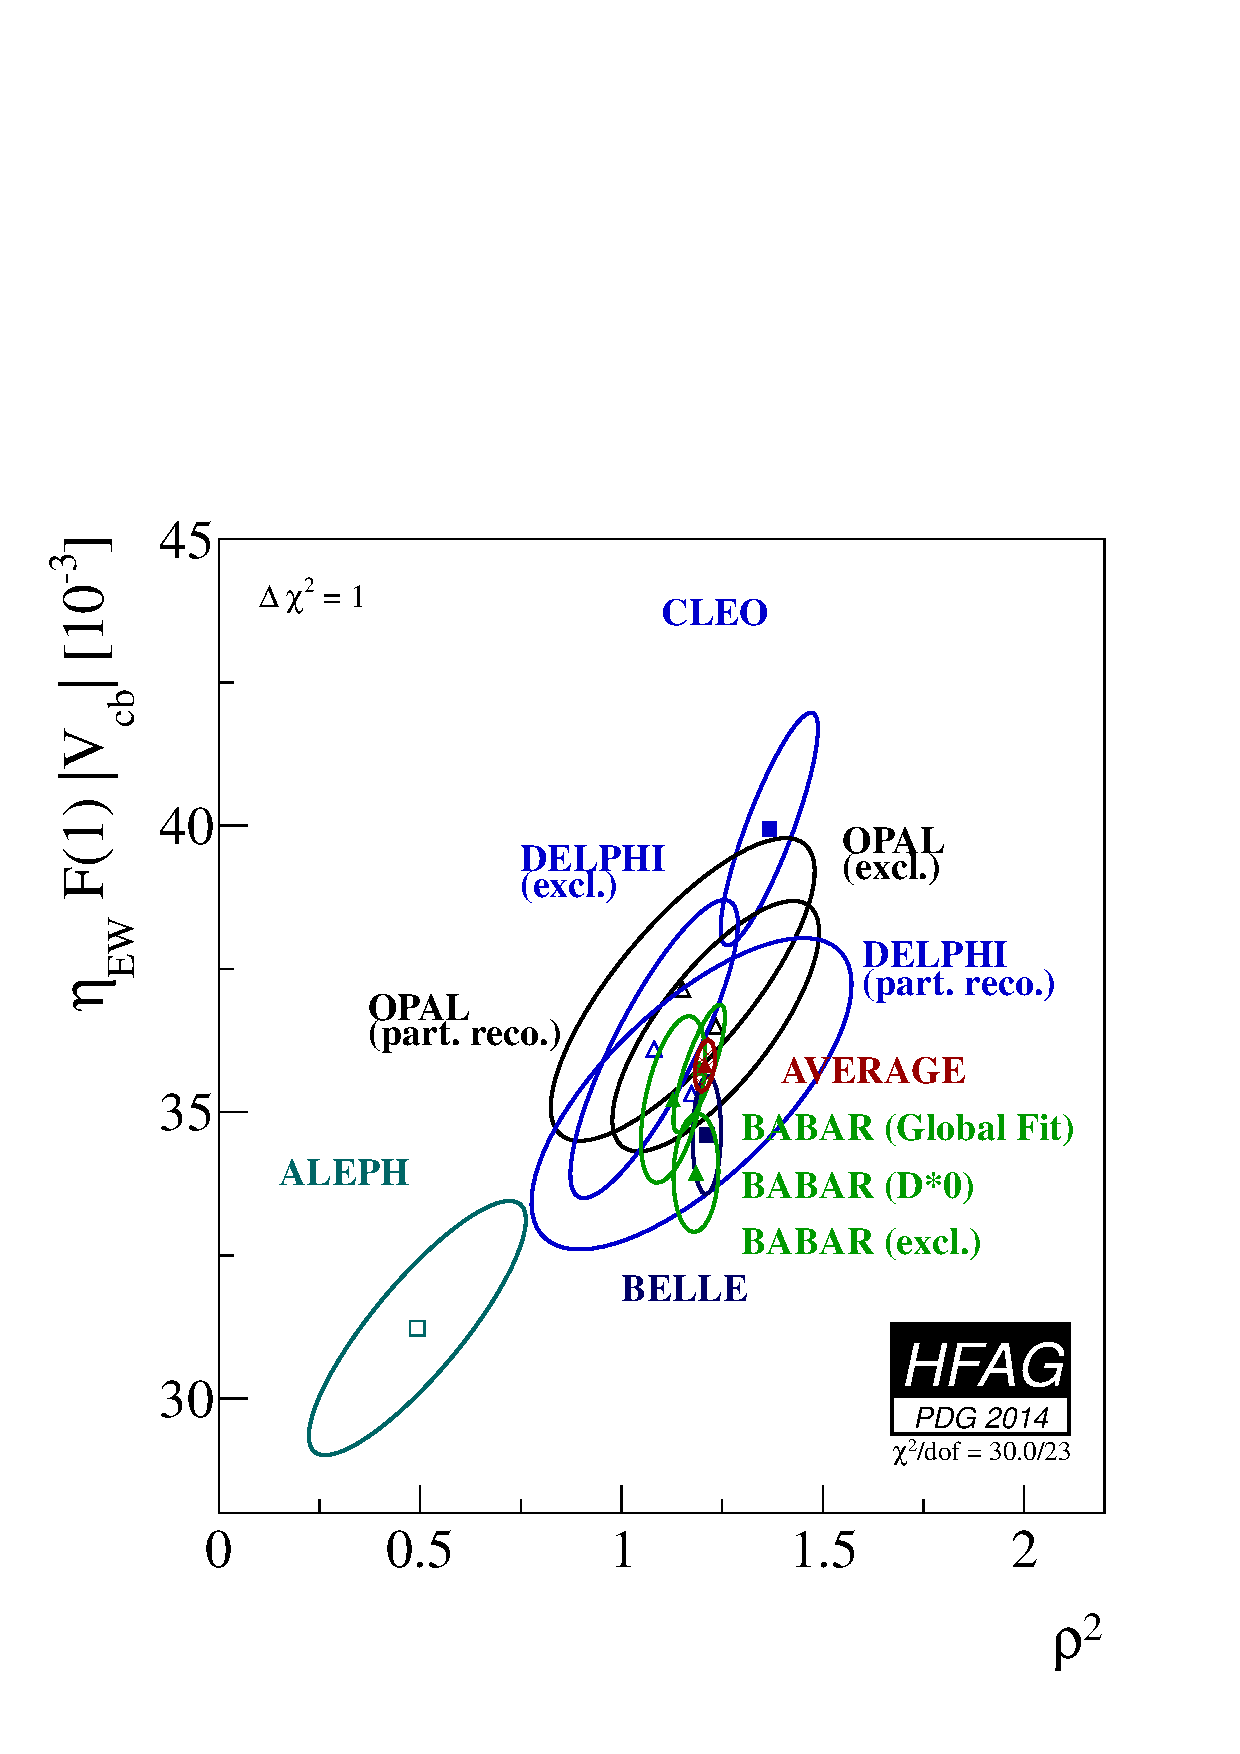
\includegraphics[width=8.0cm]{figures/slb/vcbf1_vs_rho2.pdf}
    }
    \put( -0.5,
    0.0){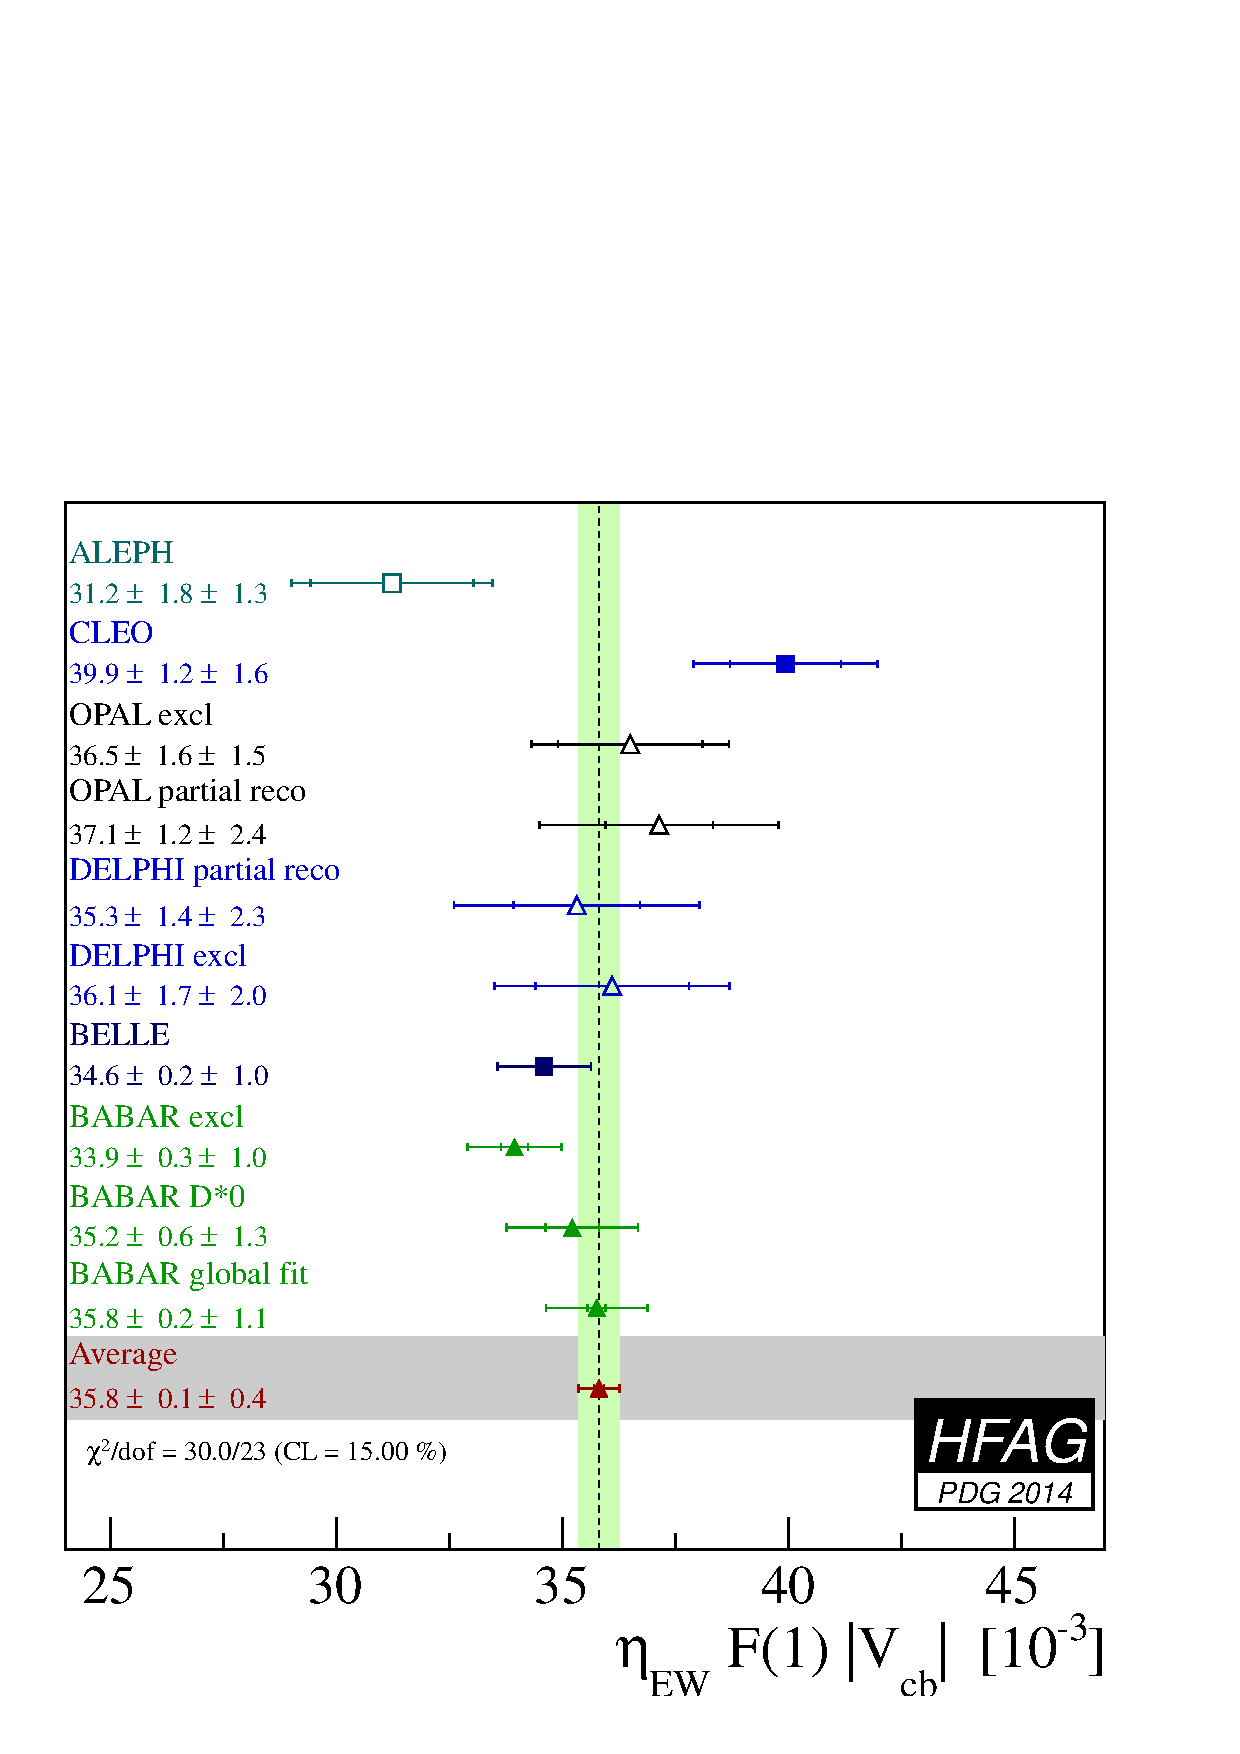
\includegraphics[width=7.5cm]{figures/slb/vcbf1.pdf}
    }
    \put(  5.5,  6.8){{\large\bf a)}}  
    \put( 14.4,  6.8){{\large\bf b)}}
  \end{picture}
  \caption{(a) Illustration of the $\eta_\mathrm{EW}{\cal F}(1)\vcb$
      average. (b) Illustration of the $\eta_\mathrm{EW}{\cal
        F}(1)\vcb$ vs.\ $\rho^2$ average. The error ellipses
      correspond  to $\Delta\chi^2 = 1$ (CL=39\%).} \label{fig:vcbf1}
  \end{center}
\end{figure}

Using the lastest update from the FNAL/MILC
group~\cite{Bailey:2014tva}, the form factor normalization
$\eta_\mathrm{EW}{\cal F}(1)$ is
\begin{equation}
  \eta_\mathrm{EW}{\cal F}(1) = 0.920\pm 0.014~,
\end{equation}
which results in the following determination of $\vcb$ from
Eq.~\ref{eq:vcbf1},
\begin{equation}
  \vcb = (38.94\pm 0.49_{\rm exp}\pm 0.58_{\rm th})\times
  10^{-3}~, \label{eq:vcbdstar}
\end{equation}
where the first uncertainty is experimental and the second error is
theoretical (lattice QCD calculation and electro-weak correction).

From each rescaled measurement in Table~\ref{tab:vcbf1}, we
calculate the $\bar B\to D^*\ell^-\bar\nu_\ell$ form factor
$\eta_\mathrm{EW}{\cal F}(w)$ and, by numerical integration, the
branching ratio of the decay $\bar B^0\to
D^{*+}\ell^-\bar\nu_\ell$. For measurements which do not determine the
parameters $R_1(1)$ and $R_2(1)$ we assume the average
values~Eqs.~\ref{eq:r1} and \ref{eq:r2}. The results are quoted in
Table~\ref{tab:dstarlnu}. The branching ratio found for the average
values of $\eta_\mathrm{EW}{\cal F}(1)\vcb$, $\rho^2$, $R_1(1)$ and
$R_2(1)$ is
\begin{equation}
  \cbf(\BzbDstarlnu)=(4.93\pm 0.11)\%~.
\end{equation}

To test isospin symmetry, we have performed a simple 1-dimensional
average of measurements sensitive to the decay $B^-\to
D^{*0}\ell^-\bar\nu_\ell$ only, which is shown in
Table~\ref{tab:dstar0lnu}. Fig.~\ref{fig:brdsl} illustrates our two
averages of $\bar B\to D^*\ell^-\bar\nu_\ell$.
\input{tables/slb/dstarlnu.tex}
\input{tables/slb/dstar0lnu.tex}
\begin{figure}[!ht]
  \begin{center}
  \unitlength1.0cm % coordinates in cm
  \begin{picture}(14.,8.0)  %ys(25.,6.0)
    \put( -0.5, 0.0){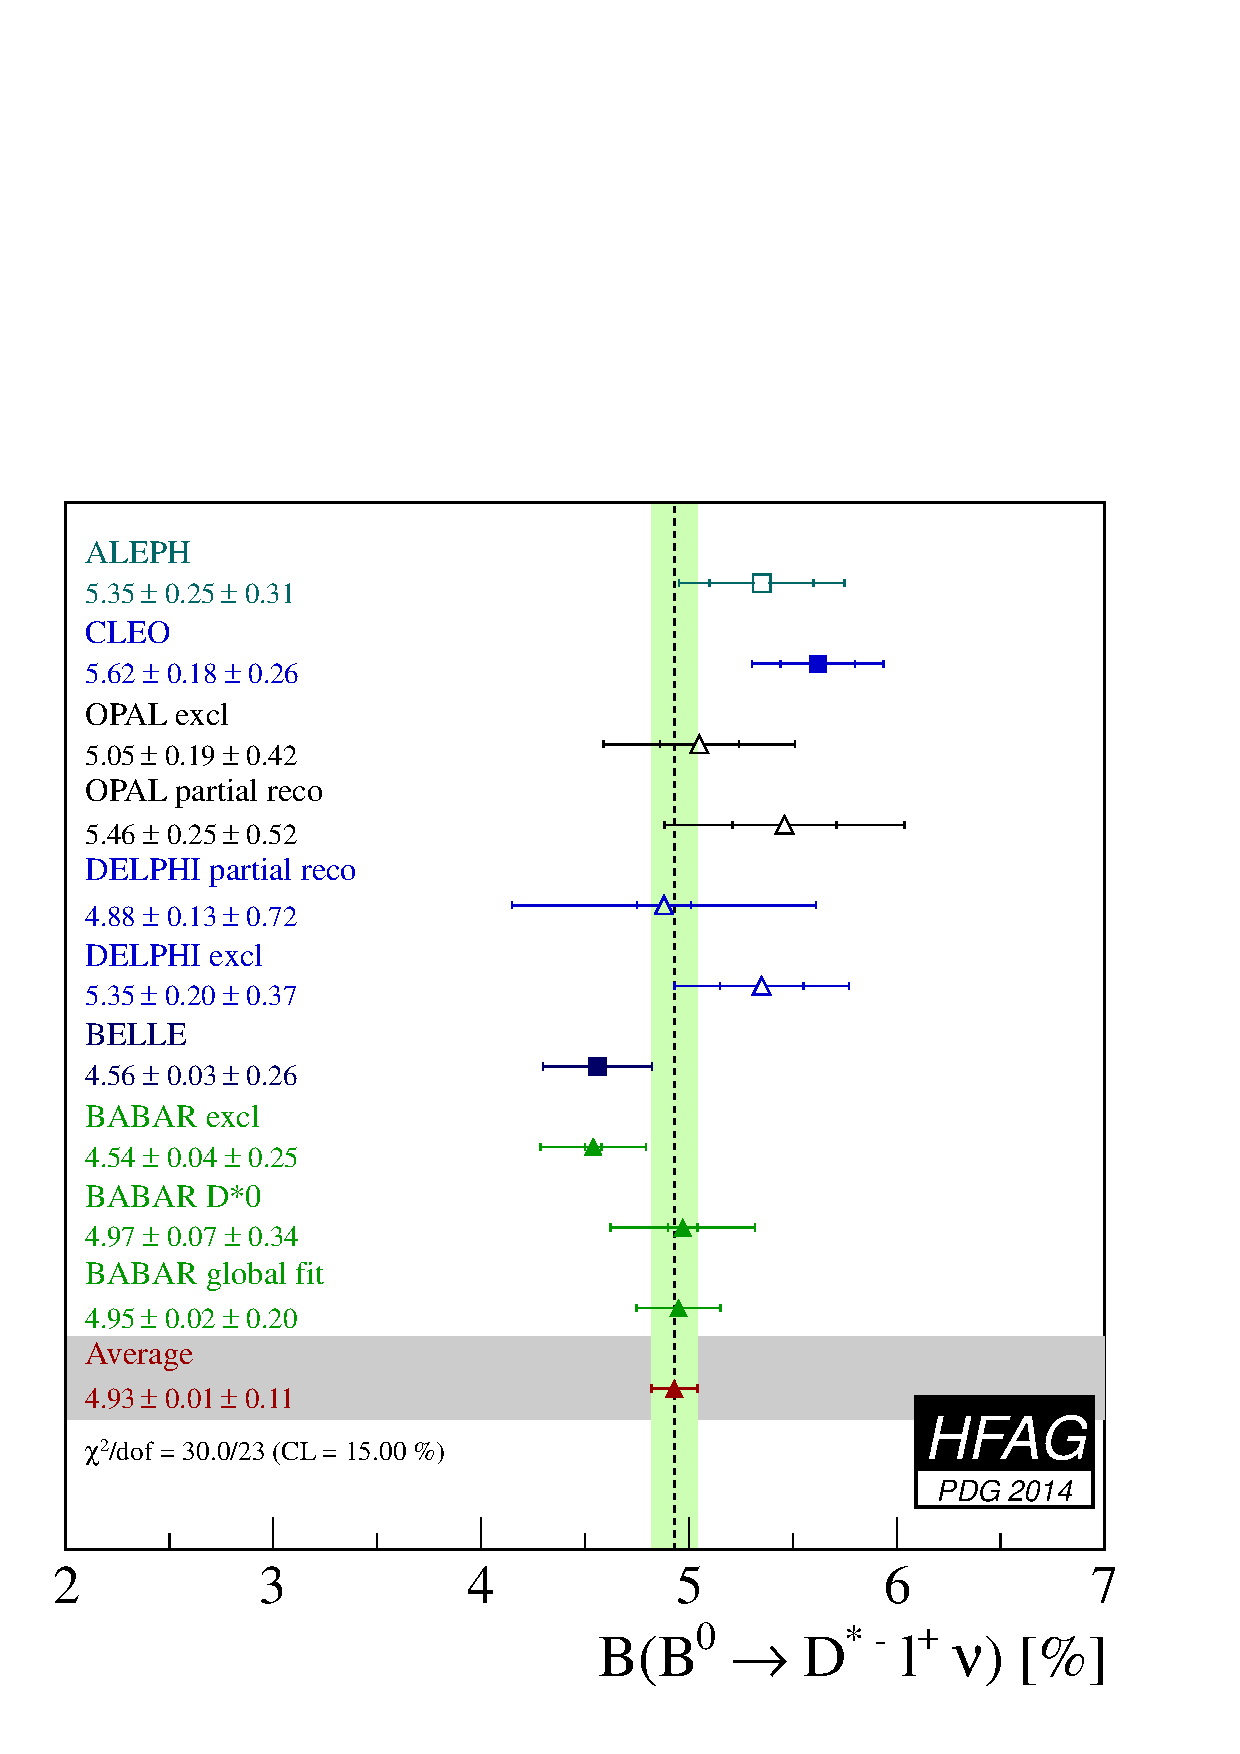
\includegraphics[width=7.5cm]{figures/slb/br_dsl_iso.pdf}
    }
    \put(  8.0, 0.0){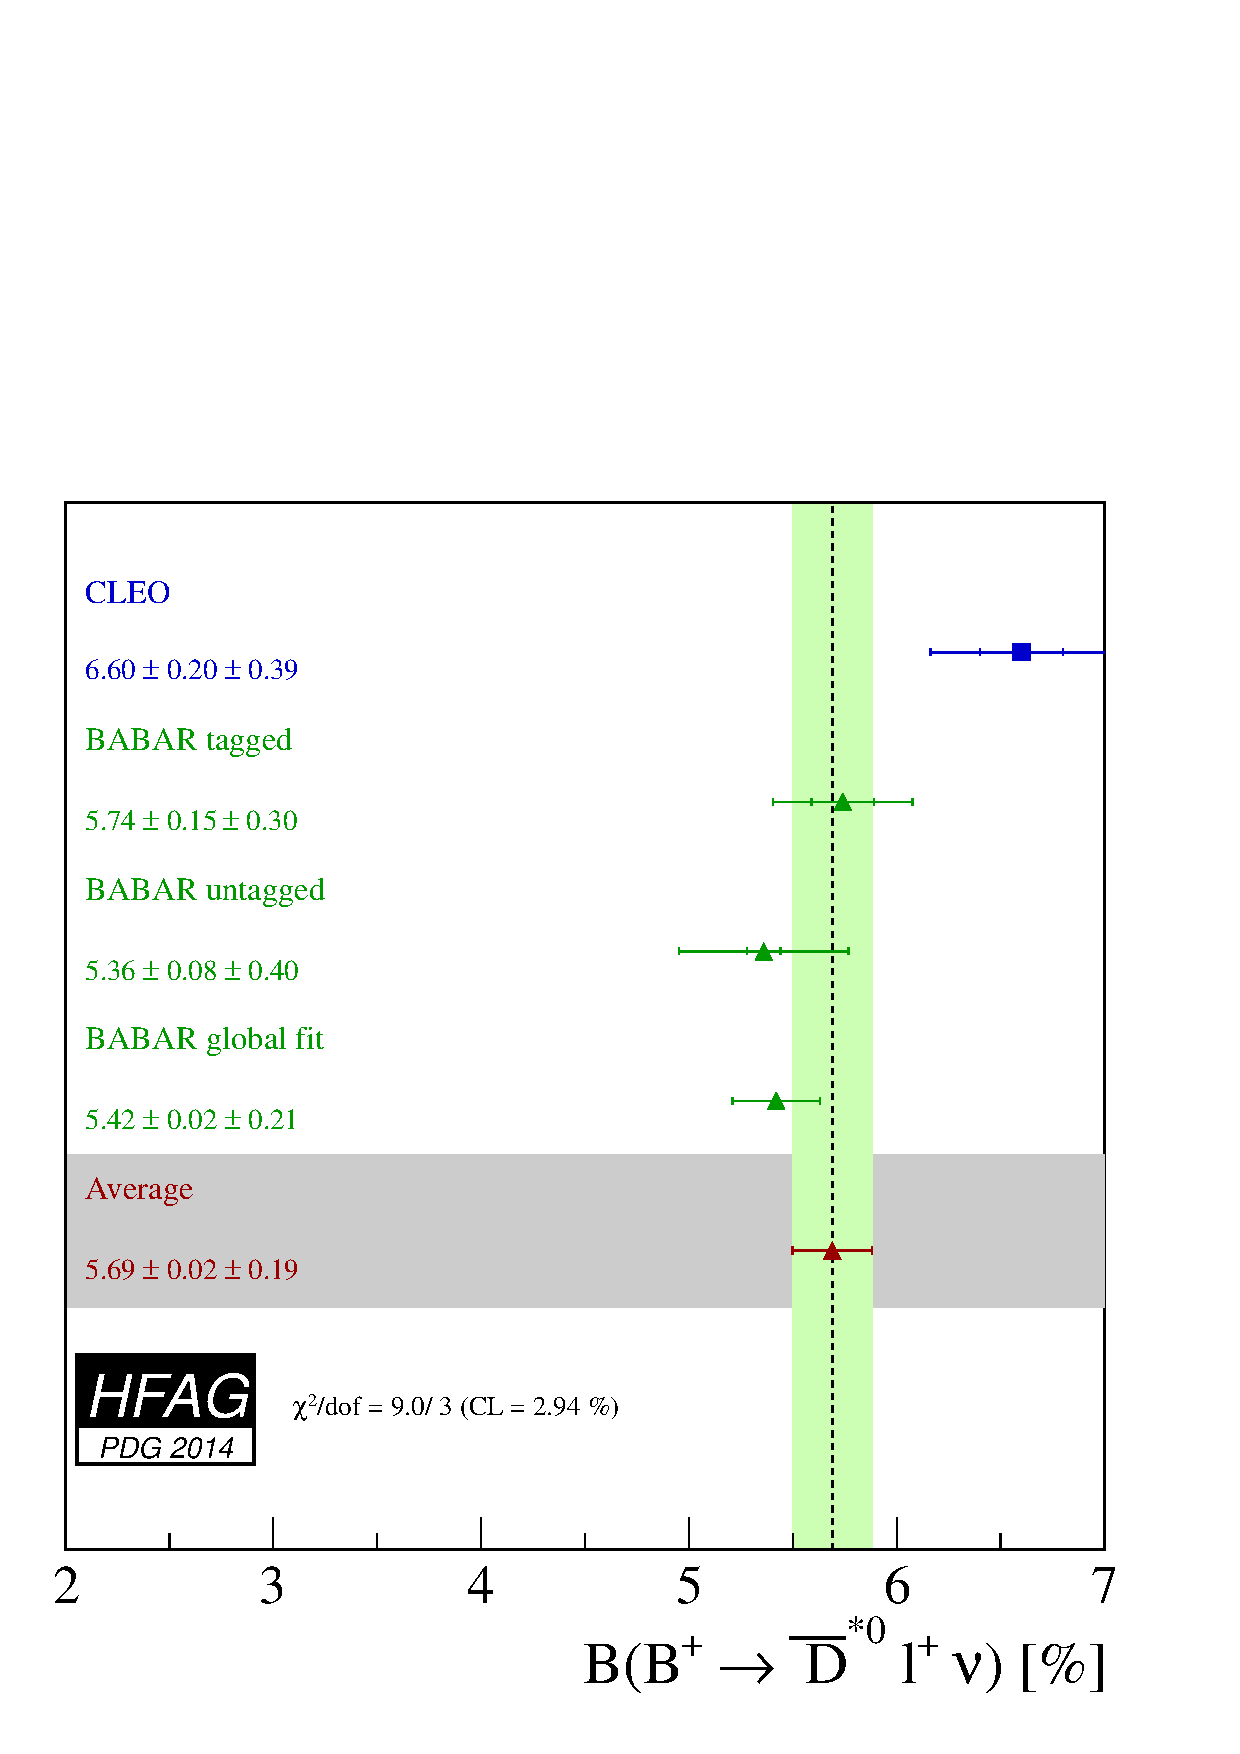
\includegraphics[width=7.5cm]{figures/slb/br_ds0l.pdf}
    }
    \put(  5.5, 6.8){{\large\bf a)}}
    \put( 14.0, 6.8){{\large\bf b)}}
  \end{picture}
  \caption{(a) Average branching fractions of exclusive semileptonic
    $B$ decays $\bar B\to D^*\ell^-\bar\nu_\ell$: (a) $\BzbDstarlnu$
    (Table~\ref{tab:dstarlnu}) and (b) $B^-\to
    D^{*0}\ell^-\bar\nu_\ell$ (Table~\ref{tab:dstar0lnu}).} \label{fig:brdsl}
  \end{center}
\end{figure}

\mysubsubsection{$\bar B\to D\ell^-\bar\nu_\ell$}
\label{slbdecays_dlnu}

The relevant form factor for the decay $\bar B\to D\ell^-\bar\nu_\ell$
is $\eta_\mathrm{EW}{\cal G}(w)$, which in CLN~\cite{CLN} is described
by only two parameters: the normalization $\eta_\mathrm{EW}{\cal
  G}(1)\vcb$ and the slope $\rho^2$.

We use the measurements of these two form factor parameters shown in
Table~\ref{tab:vcbg1} and correct them to match the latest values of
the input parameters~\cite{HFAG_sl:inputparams}. These measurements
are sensitive to both isospin states ($\BzbDplnu$ and $B^-\to
D^0\ell^-\bar\nu_\ell$). So, isospin symmetry is assumed in the analysis.
\input{tables/slb/vcbg1.tex}

The form factor parameters are extracted by a two-dimensional fit to
the rescaled measurements of $\eta_\mathrm{EW}{\cal G}(1)\vcb$ and
$\rho^2$ taking into account correlated statistical and systematic
uncertainties. The result of the fit reads
\begin{eqnarray}
  \eta_\mathrm{EW}{\cal G}(1)\vcb & = & (42.65\pm 1.53)\times
  10^{-3}~, \label{eq:vcbg1} \\
  \rho^2 & = & 1.185 \pm 0.054~,
\end{eqnarray}
with a correlation of
\begin{equation}
  \rho_{\eta_\mathrm{EW}{\cal G}(1)\vcb,\rho^2} = 0.824~.
\end{equation}
The uncertainties and the correlation coefficient include both
statistical and systematic contributions. The $\chi^2$ of the fit is
0.5 for 8 degrees of freedom, which corresponds to a confidence
level of 100.0\%. An illustration of this fit result is given in
Fig.~\ref{fig:vcbg1}.
\begin{figure}[!ht]
  \begin{center}
  \unitlength1.0cm % coordinates in cm
  \begin{picture}(14.,8.) %ys(25.,6.)
    \put(  8.0, -0.2){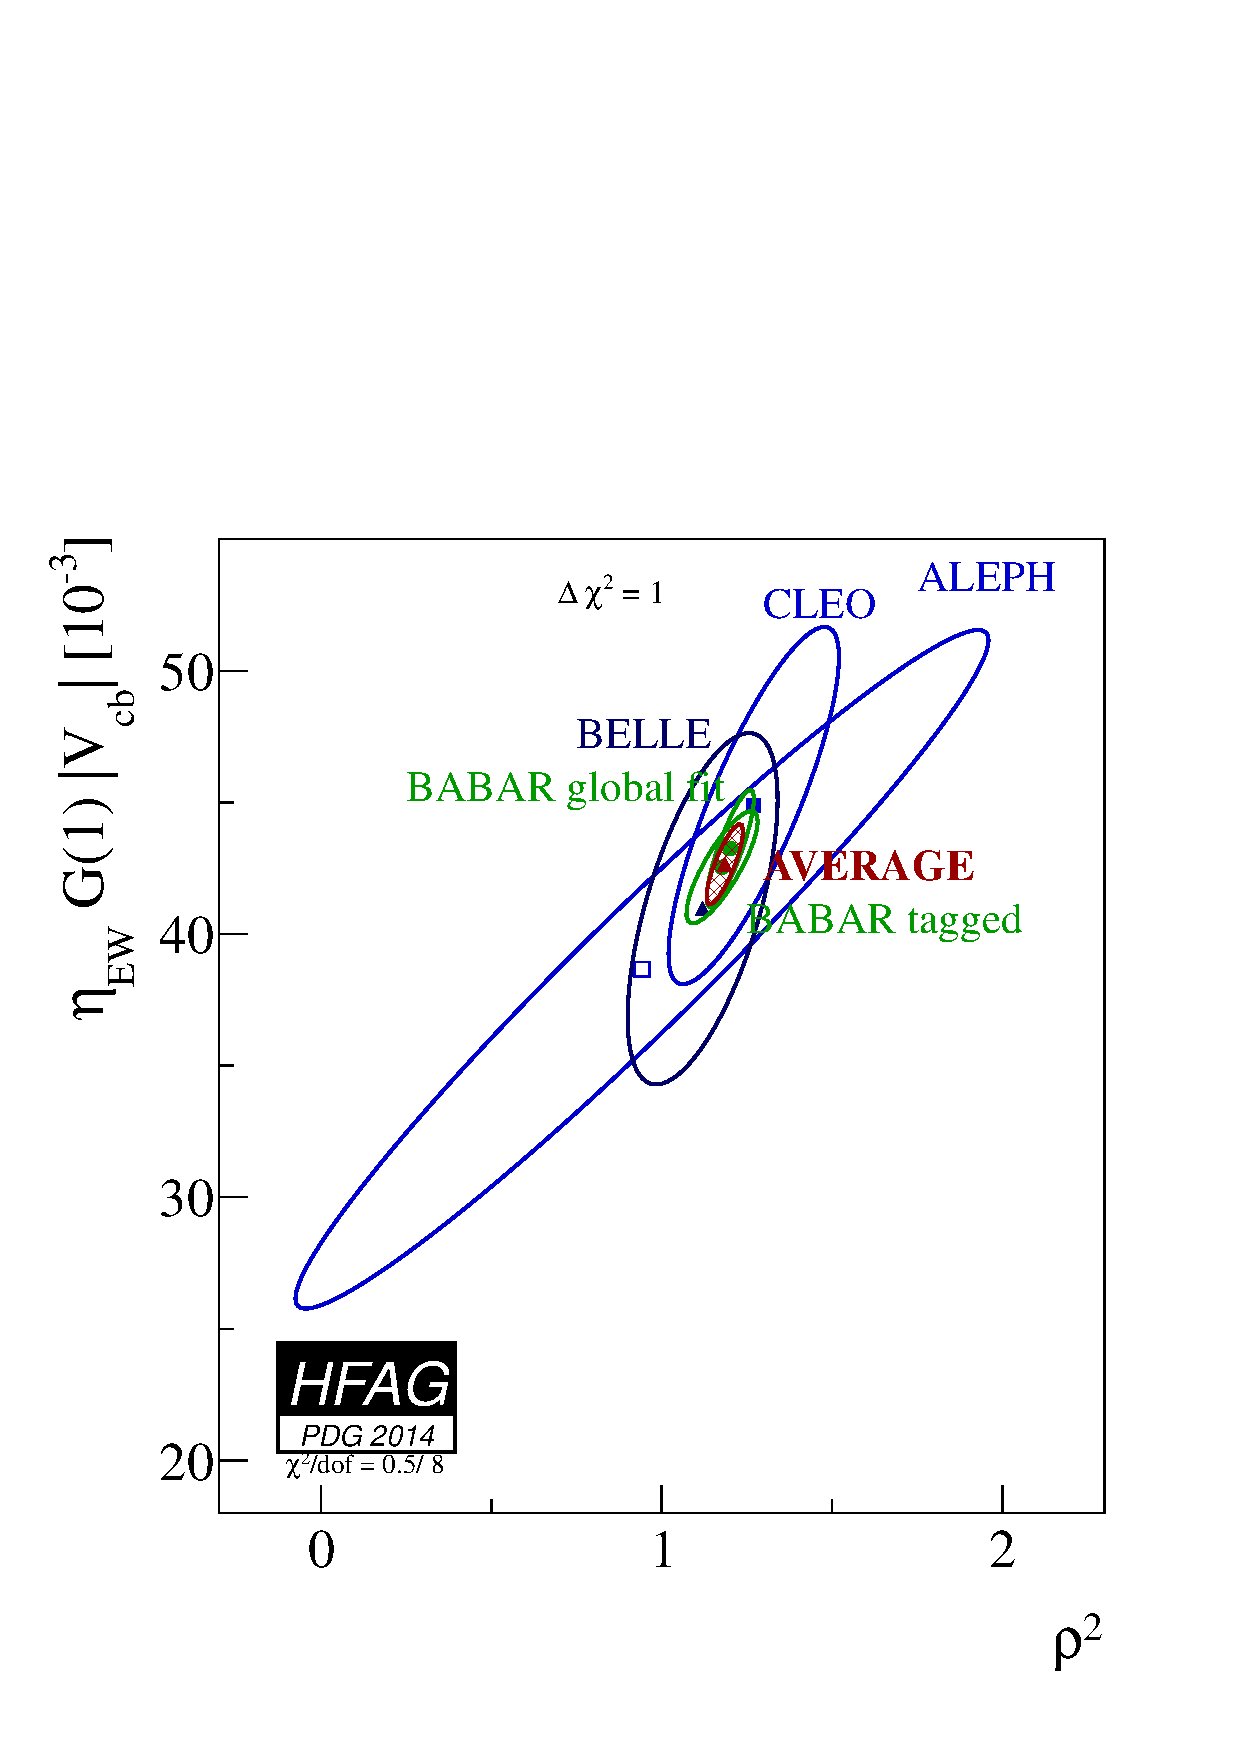
\includegraphics[width=8.0cm]{figures/slb/vcbg1_vs_rho2.pdf}
    }
    \put( -0.5,  0.0){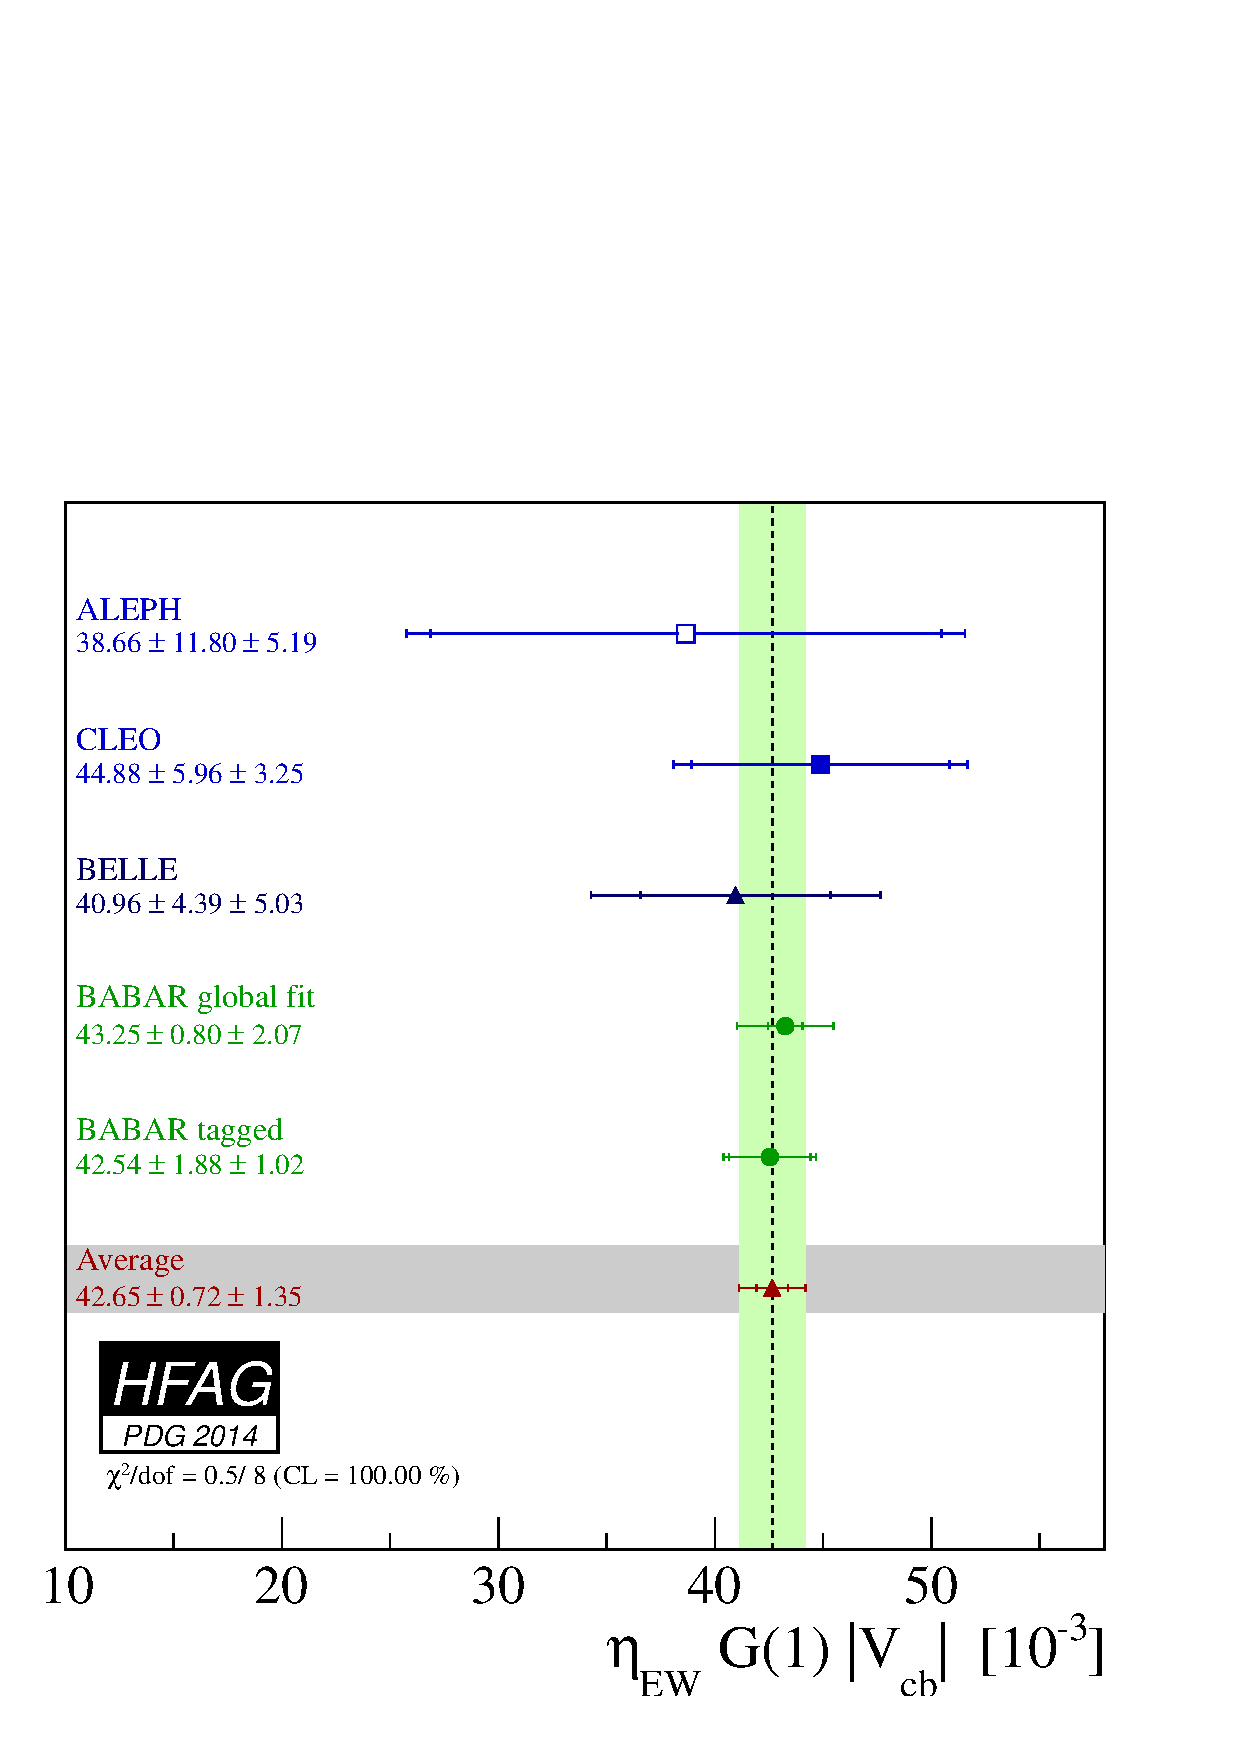
\includegraphics[width=7.5cm]{figures/slb/vcbg1.pdf}
    }
    \put(  5.5,  6.8){{\large\bf a)}}
    \put( 9.4,  6.8){{\large\bf b)}}
  \end{picture}
  \caption{(a) Illustration of the $\eta_\mathrm{EW}{\cal G}(1)\vcb$
    average. (b) Illustration of the $\eta_\mathrm{EW}{\cal G}(1)\vcb$
    vs.\ $\rho^2$ average. The error ellipses correspond  to
    $\Delta\chi^2 = 1$ (CL=39\%).}
  \label{fig:vcbg1}
  \end{center}
\end{figure}

The most recent lattice QCD result obtained for the form factor
normalization $\eta_\mathrm{EW}{\cal G}(1)$ is~\cite{Okamoto:2004xg}
\begin{equation}
  \eta_\mathrm{EW}{\cal G}(1) = 1.081\pm 0.024~,
\end{equation}
which can be used to turn Eq.~\ref{eq:vcbg1} into a determination of
$\vcb$,
\begin{equation}
  \vcb = (39.45\pm 1.42_{\rm exp}\pm 0.88_{\rm th})\times 10^{-3}~,
\end{equation}
where the first error is experimental and the second theoretical. This
number is in excellent agreement with $\vcb$ obtained from decays
$\bar B\to D^*\ell^-\bar\nu_\ell$ (Eq.~\ref{eq:vcbdstar}).

From each rescaled measurement in Table~\ref{tab:vcbg1}, we have
calculated the $\bar B\to D\ell^-\bar\nu_\ell$ form factor ${\cal
  G}(w)$ and, by numerical integration, the branching ratio of the
decay $\BzbDplnu$. The results are quoted in Table~\ref{tab:dlnuIso} and
illustrated in Fig.~\ref{fig:brdlIso}. The branching ratio found for
the average values of $\eta_\mathrm{EW}{\cal G}(1)\vcb$ and $\rho^2$ is
\begin{equation}
  \cbf(\BzbDplnu)=(2.13\pm 0.09)\%~.
\end{equation}
\input{tables/slb/dlnuIso.tex}
\begin{figure}[!ht]
  \begin{center}
    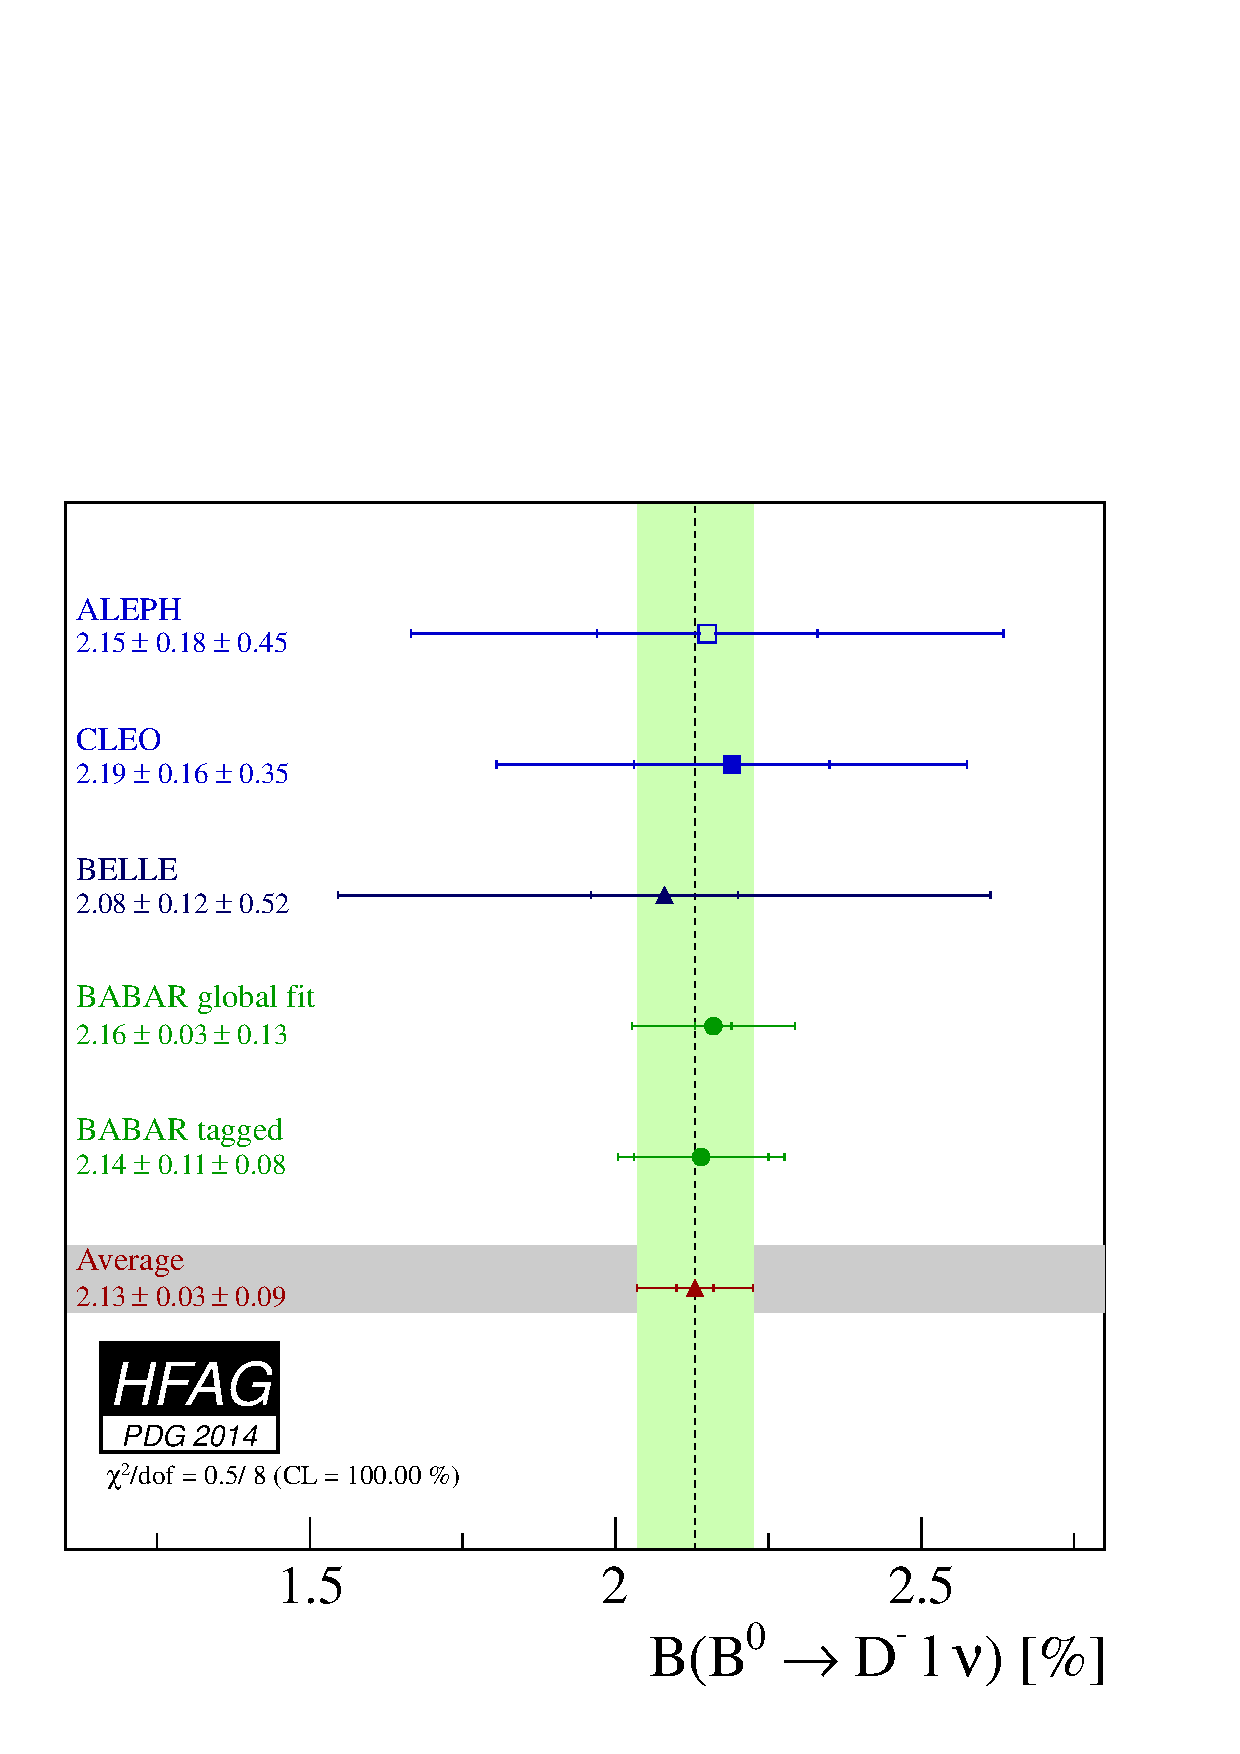
\includegraphics[width=7.55cm]{figures/slb/br_dl_iso.pdf}
    \caption{Illustration of Table~\ref{tab:dlnuIso}.} \label{fig:brdlIso}
  \end{center}
\end{figure}

We have also performed simple 1-dimensional averages of measurements
of $\BzbDplnu$ and $B^-\to D^0\ell^-\bar\nu_\ell$. These fits are
shown Tables~\ref{tab:dlnu} and \ref{tab:d0lnu}.
\input{tables/slb/dlnu.tex}
\input{tables/slb/d0lnu.tex}

%===================================================================
% D** 
%===================================================================

\mysubsubsection{$\bar{B} \to D^{(*)}\pi \ell^-\bar{\nu}_{\ell}$}
\label{slbdecays_dpilnu}
% --------------------

The average inclusive branching fractions for $\bar{B} \to D^{*}\pi \ell^-\bar{\nu}_{\ell}$
decays, where no constrain is applied to the hadronic $D^{(*)}\pi$ system, 
are determined by the
combination of the results provided in Table~\ref{tab:dpilnu} for 
$\bar{B}^0 \to D^0 \pi^+ \ell^-\bar{\nu}_{\ell}$, $\bar{B}^0 \to D^{*0} \pi^+
\ell^-\bar{\nu}_{\ell}$, 
$B^- \to D^+ \pi^-
\ell^-\bar{\nu}_{\ell}$, and $B^- \to D^{*+} \pi^- \ell^-\bar{\nu}_{\ell}$.
The measurements included in the average 
are scaled to a consistent set of input
parameters and their errors~\cite{HFAG_sl:inputparams}.
For both the \babar\ and Belle results, the $B$ semileptonic signal yields are
 extracted from a fit to the missing mass squared in a sample of fully
 reconstructed \BB\ events.  
Figure~\ref{fig:brdpil} illustrates the measurements and the
resulting average.

\input{tables/slb/dpilnu.tex}

\begin{figure}[!ht]
 \begin{center}
  \unitlength1.0cm % coordinates in cm
  \begin{picture}(14.,8.0)  %ys(25.,6.0)
   \put( -0.5,  0.0){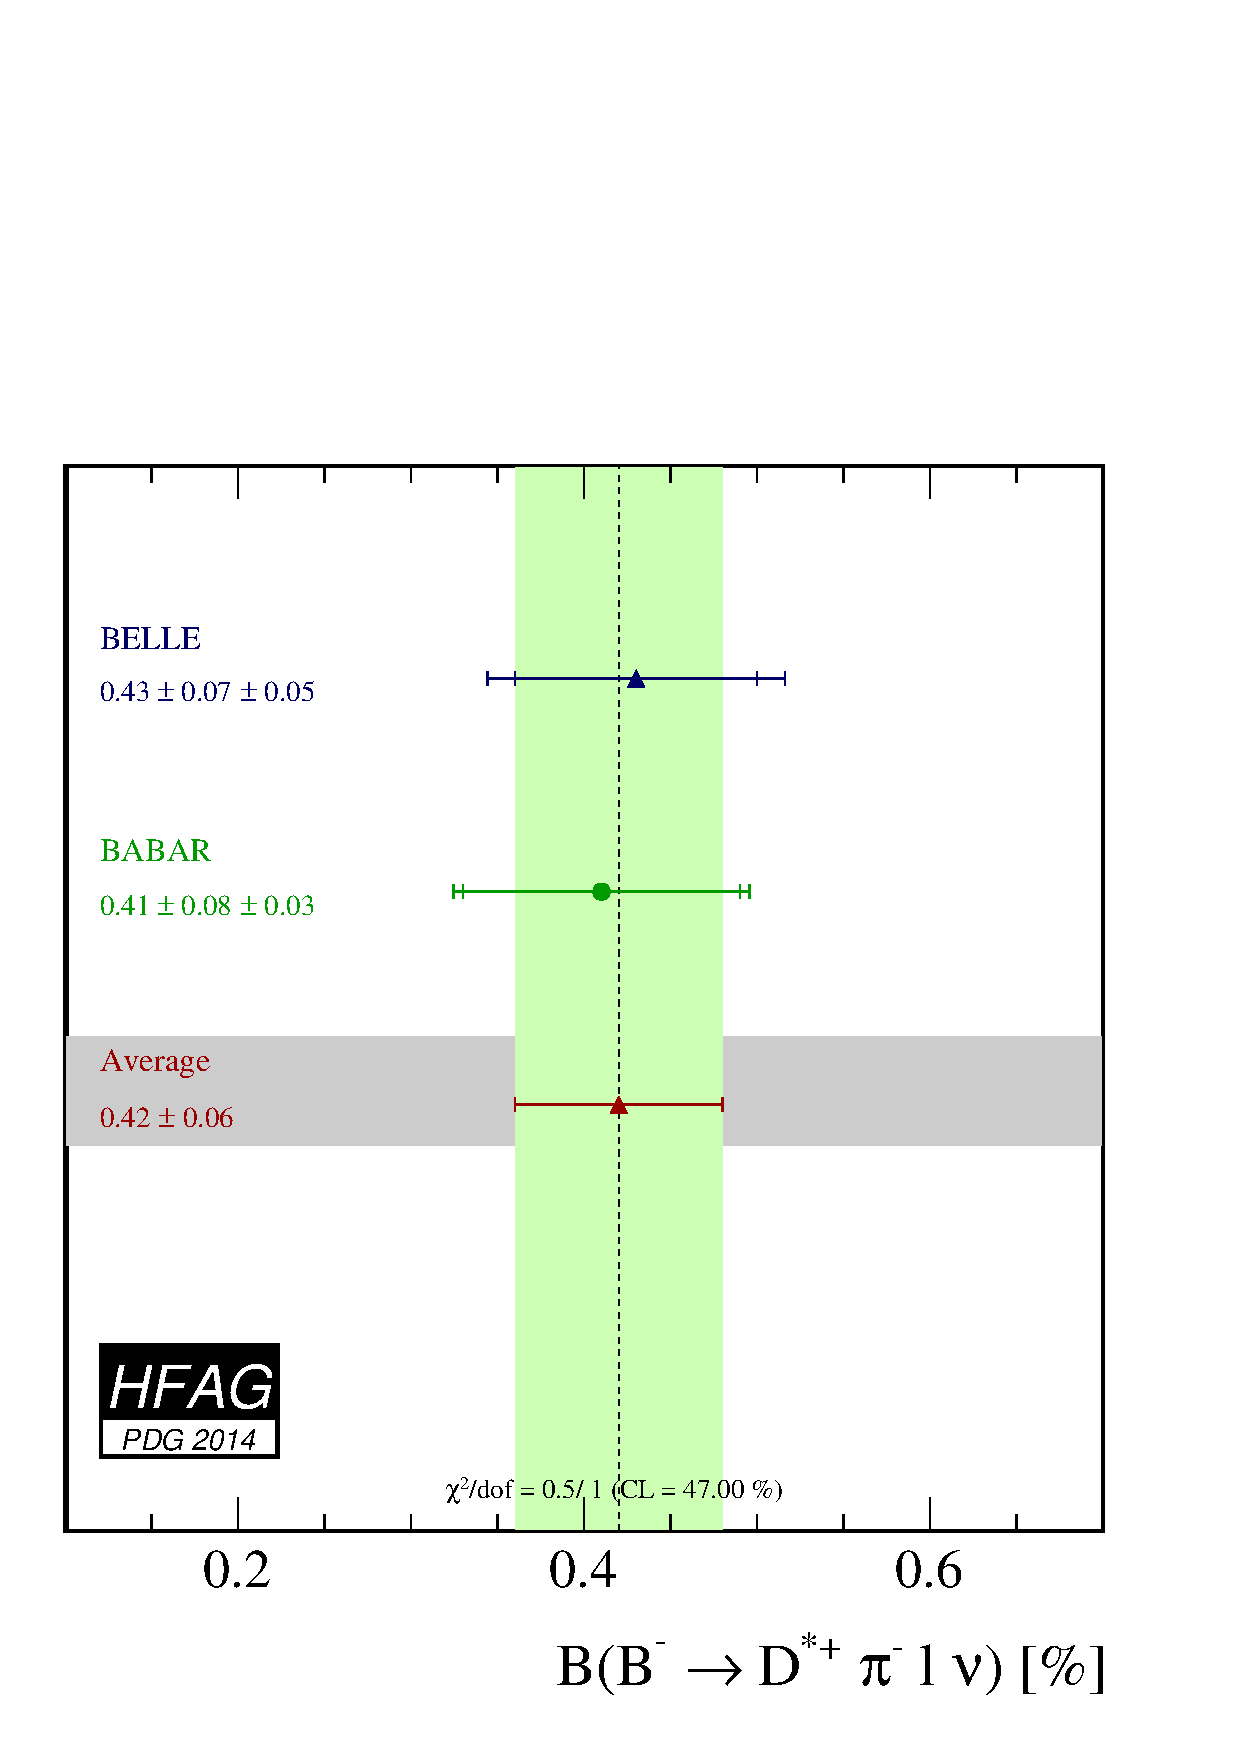
\includegraphics[width=7.55cm]{figures/slb/br_dssIncl-3.pdf}
   }
   \put(  8.0,  0.0){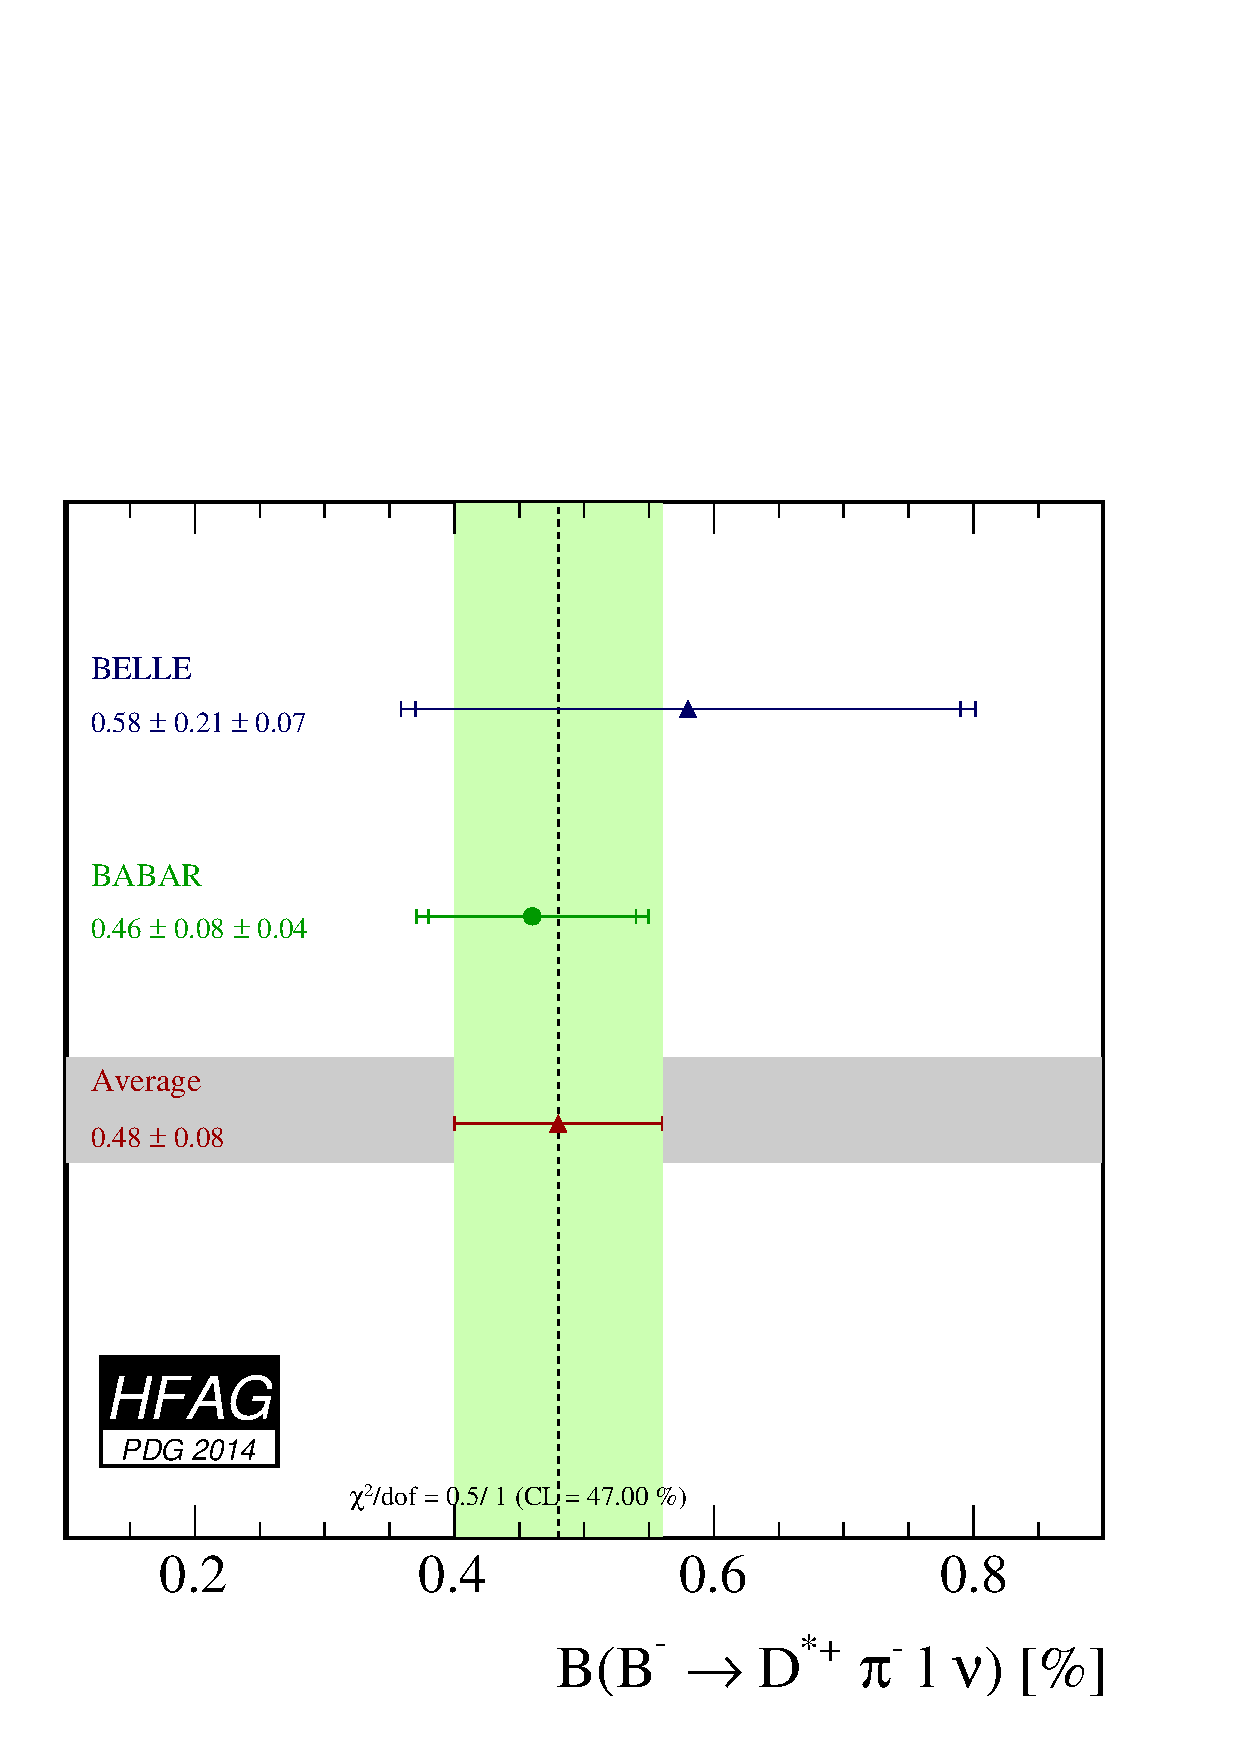
\includegraphics[width=7.8cm]{figures/slb/br_dssIncl-4.pdf}
   }
   \put(  5.5,  6.8){{\large\bf a)}}
   \put( 14.0,  6.8){{\large\bf b)}}
  \end{picture}
  \begin{picture}(14.,8.0)  %ys(25.,6.0)
   \put( -0.5,  0.0){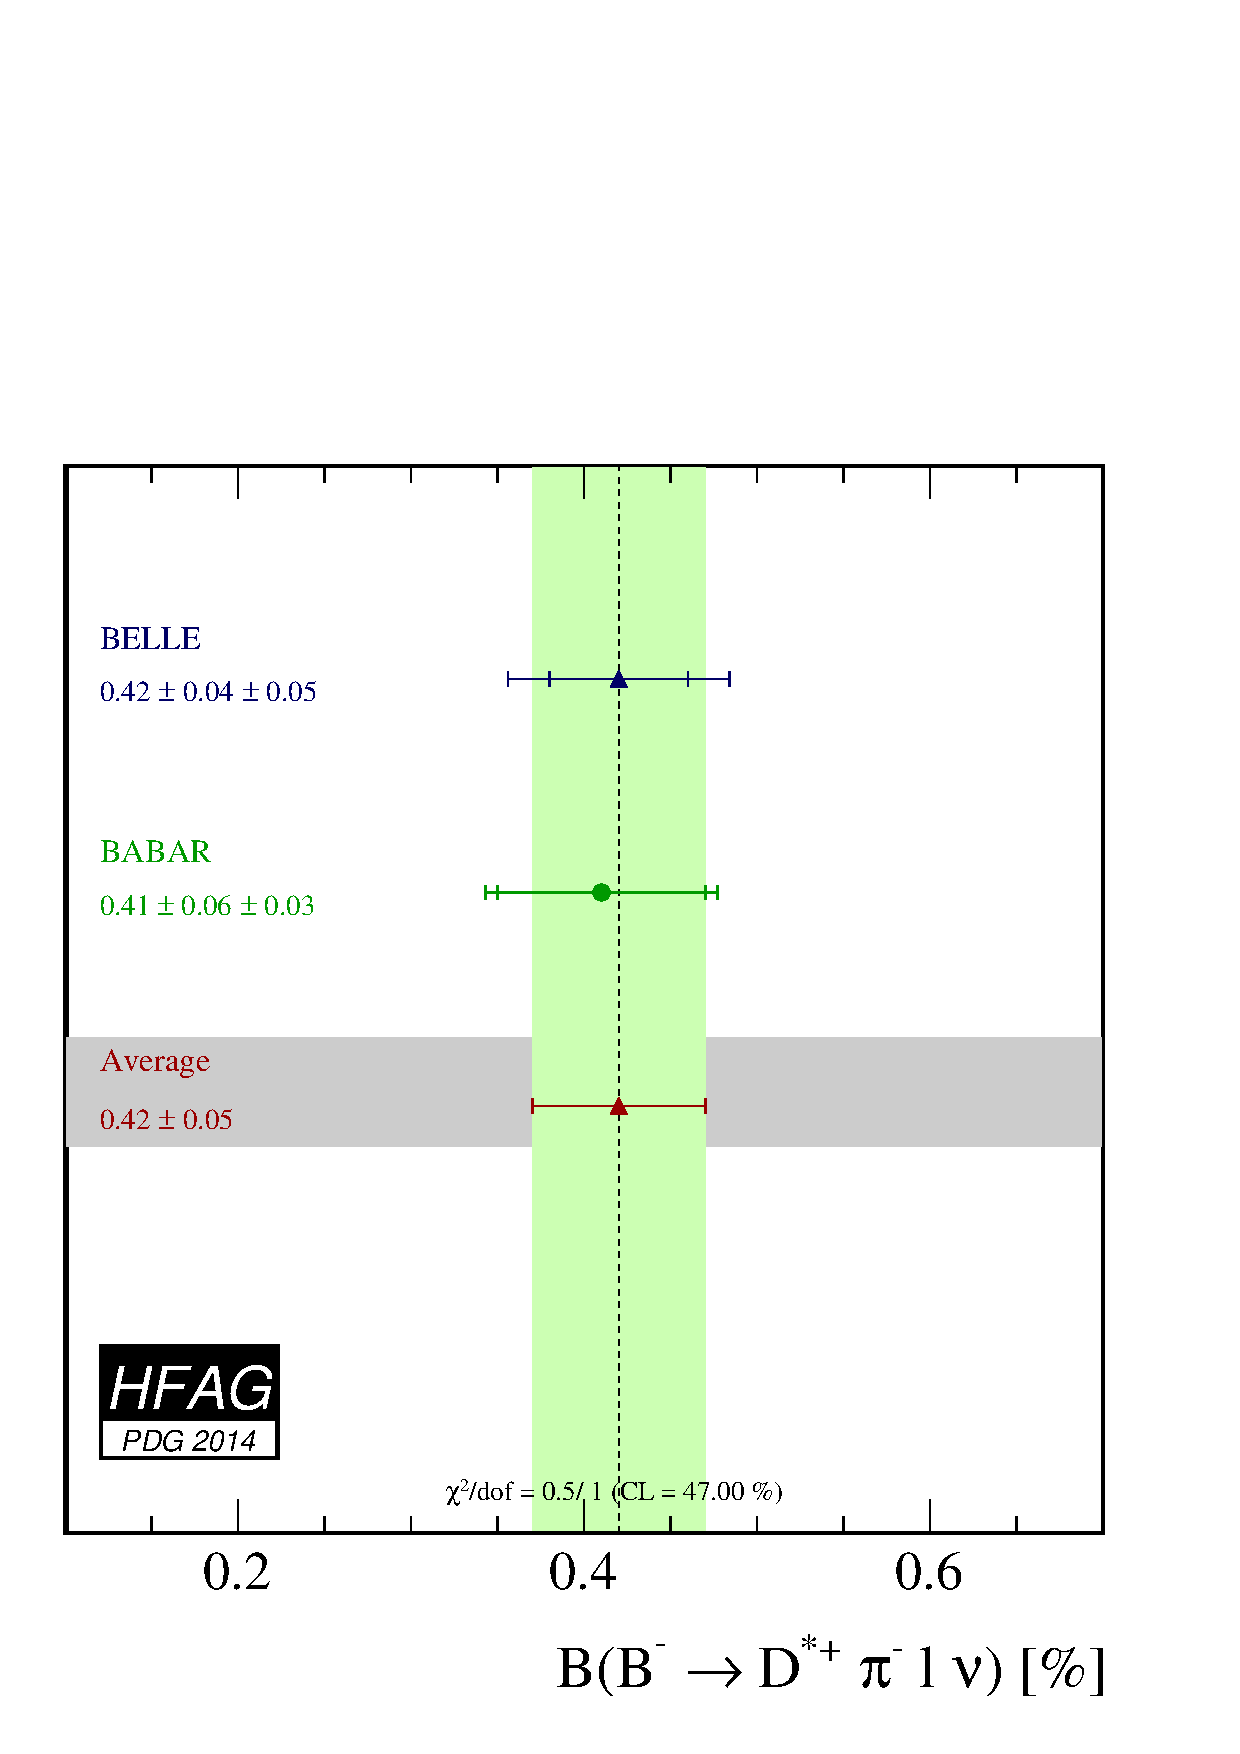
\includegraphics[width=7.55cm]{figures/slb/br_dssIncl-1.pdf}
   }
   \put(  8.0,  0.0){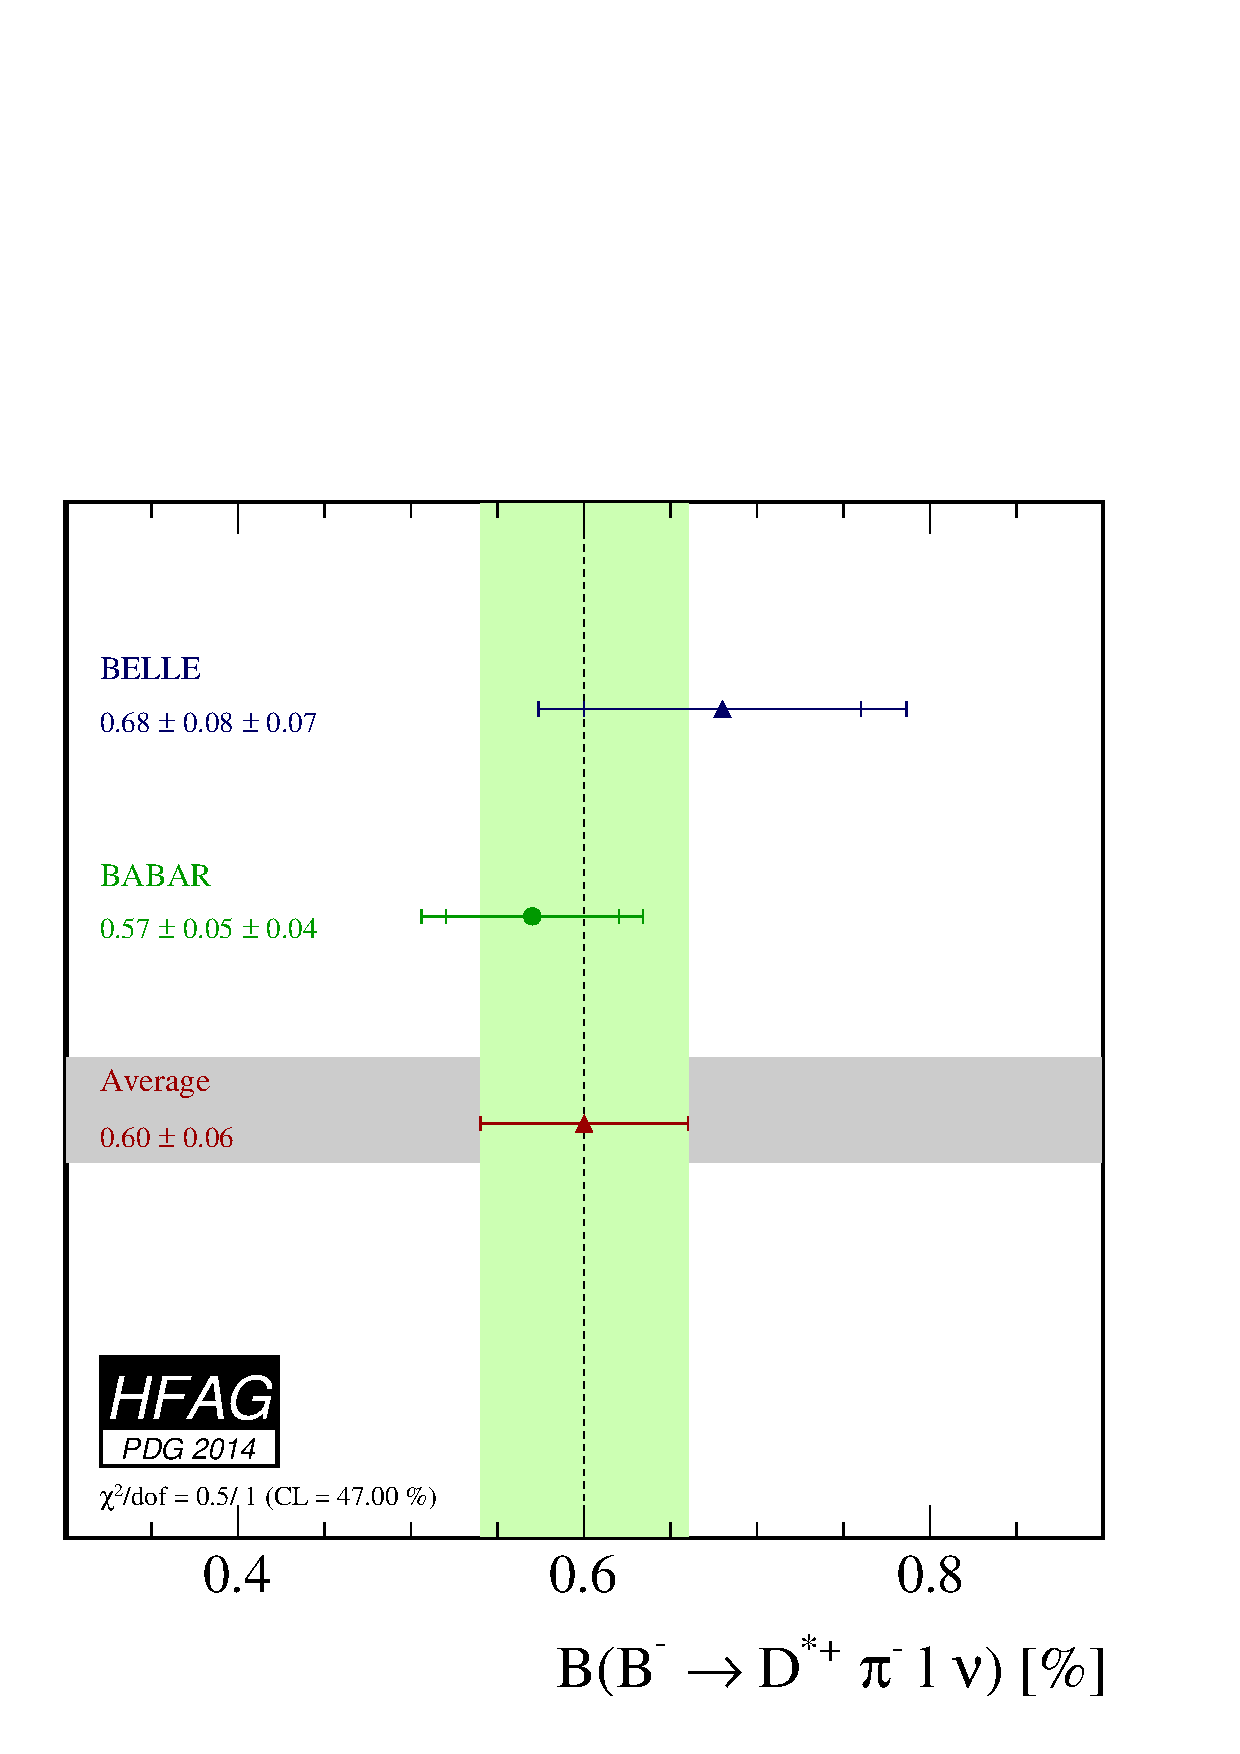
\includegraphics[width=7.8cm]{figures/slb/br_dssIncl-2.pdf}
   }
   \put(  5.5,  6.8){{\large\bf c)}}
   \put( 14.0,  6.8){{\large\bf d)}}
  \end{picture}
  \caption{Average branching fraction  of exclusive semileptonic $B$ decays
(a) $\bar{B}^0 \to D^0 \pi^+ \ell^-\bar{\nu}_{\ell}$, (b) $\bar{B}^0 \to D^{*0} \pi^+
\ell^-\bar{\nu}_{\ell}$, (c) $B^- \to D^+ \pi^-
\ell^-\bar{\nu}_{\ell}$, and (d) $B^- \to D^{*+} \pi^- \ell^-\bar{\nu}_{\ell}$.
The corresponding individual
  results are also shown.}
  \label{fig:brdpil}
 \end{center}
\end{figure}

\mysubsubsection{$\bar{B} \to D^{**} \ell^-\bar{\nu}_{\ell}$}
\label{slbdecays_dsslnu}
% -------------------

The $D^{**}$ mesons contain one charm quark and one light quark with relative angular momentum $L=1$. According to Heavy Quark Symmetry (HQS)~\cite{Isgur:1991wq}, they form one doublet of states with angular momentum $j \equiv s_q + L= 3/2$  $\left[D_1(2420), D_2^*(2460)\right]$ and another doublet with $j=1/2$ $\left[D^*_0(2400), D_1'(2430)\right]$, where $s_q$ is the light quark spin. Parity and angular momentum conservation constrain the decays allowed for each state. The $D_1$ and $D_2^*$ states decay through a D-wave to $D^*\pi$ and $D^{(*)}\pi$, respectively, and have small decay widths, while the $D_0^*$ and $D_1'$  states decay through an S-wave to $D\pi$ and $D^*\pi$ and are very broad.
For the narrow states, the average  are determined by the
combination of the results provided in Table~\ref{tab:dss1lnu} and \ref{tab:dss2lnu} for 
$\cbf(B^- \to D_1^0(D^{*+}\pi^-)\ell^-\bar{\nu}_{\ell})
\times \cbf(D_1^0 \to D^{*+}\pi^-)$ and $\cbf(B^- \to D_2^0(D^{*+}\pi^-)\ell^-\bar{\nu}_{\ell})
\times \cbf(D_2^0 \to D^{*+}\pi^-)$. 
For the broad states, the average are determined by the
combination of the results provided in Table~\ref{tab:dss1plnu} and \ref{tab:dss0lnu} for 
$\cbf(B^- \to D_1'^0(D^{*+}\pi^-)\ell^-\bar{\nu}_{\ell})
\times \cbf(D_1'^0 \to D^{*+}\pi^-)$ and $\cbf(B^- \to D_0^{*0}(D^{+}\pi^-)\ell^-\bar{\nu}_{\ell})
\times \cbf(D_0^{*0} \to D^{+}\pi^-)$. 
The measurements included in the average are scaled to a consistent set of input
parameters and their errors~\cite{HFAG_sl:inputparams}.  

For both the B-factory and the LEP and Tevatron results, the $B$ semileptonic 
signal yields are extracted from a fit to the invariant mass distribution of the $D^{(*)+}\pi^-$ system.
 Apart for the CLEO, \belle and \babar results, the other measurements 
 are for the $\bar{B} \to D^{**}(D^*\pi^-)X \ell^- \bar{\nu}_{\ell}$ final state and 
 we assume that no particles are left in the X system. The \babar tagged measurement \cite{Aubert:2009_4} measures 
 $\bar{B} \to D_2^*(D\pi)X \ell^- \bar{\nu}_{\ell}$ and it has been translated in 
 a result on  $D_2^*\to D^*\pi$ decay mode, assuming 
 ${\cal B}(D_2^*\to D\pi)/{\cal B}(D_2^*\to D^*\pi)=1.54\pm 0.15$ \cite{PDG_2014}. 
Figure~\ref{fig:brdssl} and ~\ref{fig:brdssl2} illustrate the measurements and the
resulting average.

\input{tables/slb/dss1lnu.tex}
\input{tables/slb/dss2lnu.tex}
\input{tables/slb/dss1plnu.tex}
\input{tables/slb/dss0lnu.tex}

\begin{figure}[!ht]
 \begin{center}
  \unitlength1.0cm % coordinates in cm
  \begin{picture}(14.,8.0)  %ys(25.,6.0)
   \put( -0.5,  0.0){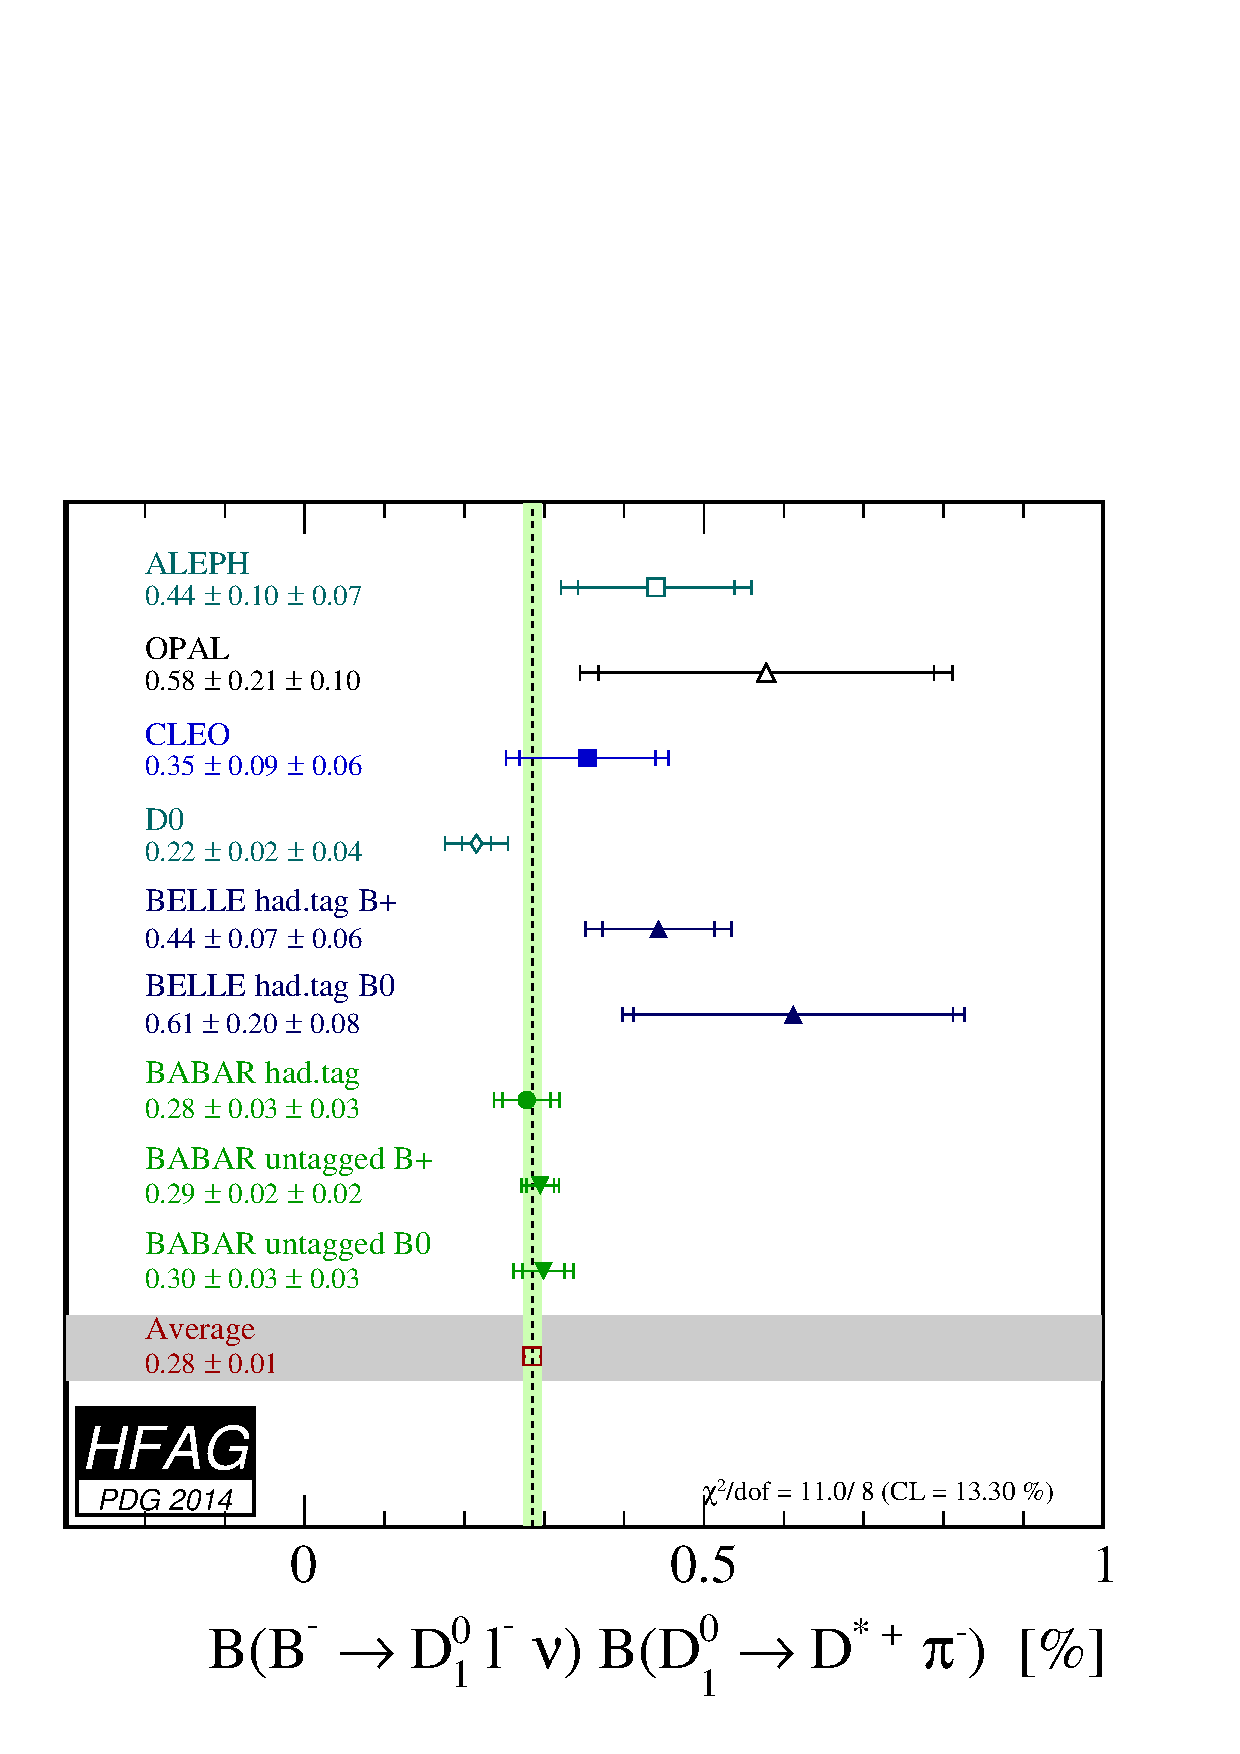
\includegraphics[width=7.8cm]{figures/slb/br_dss1l.pdf}
   }
   \put(  8.0,  0.0){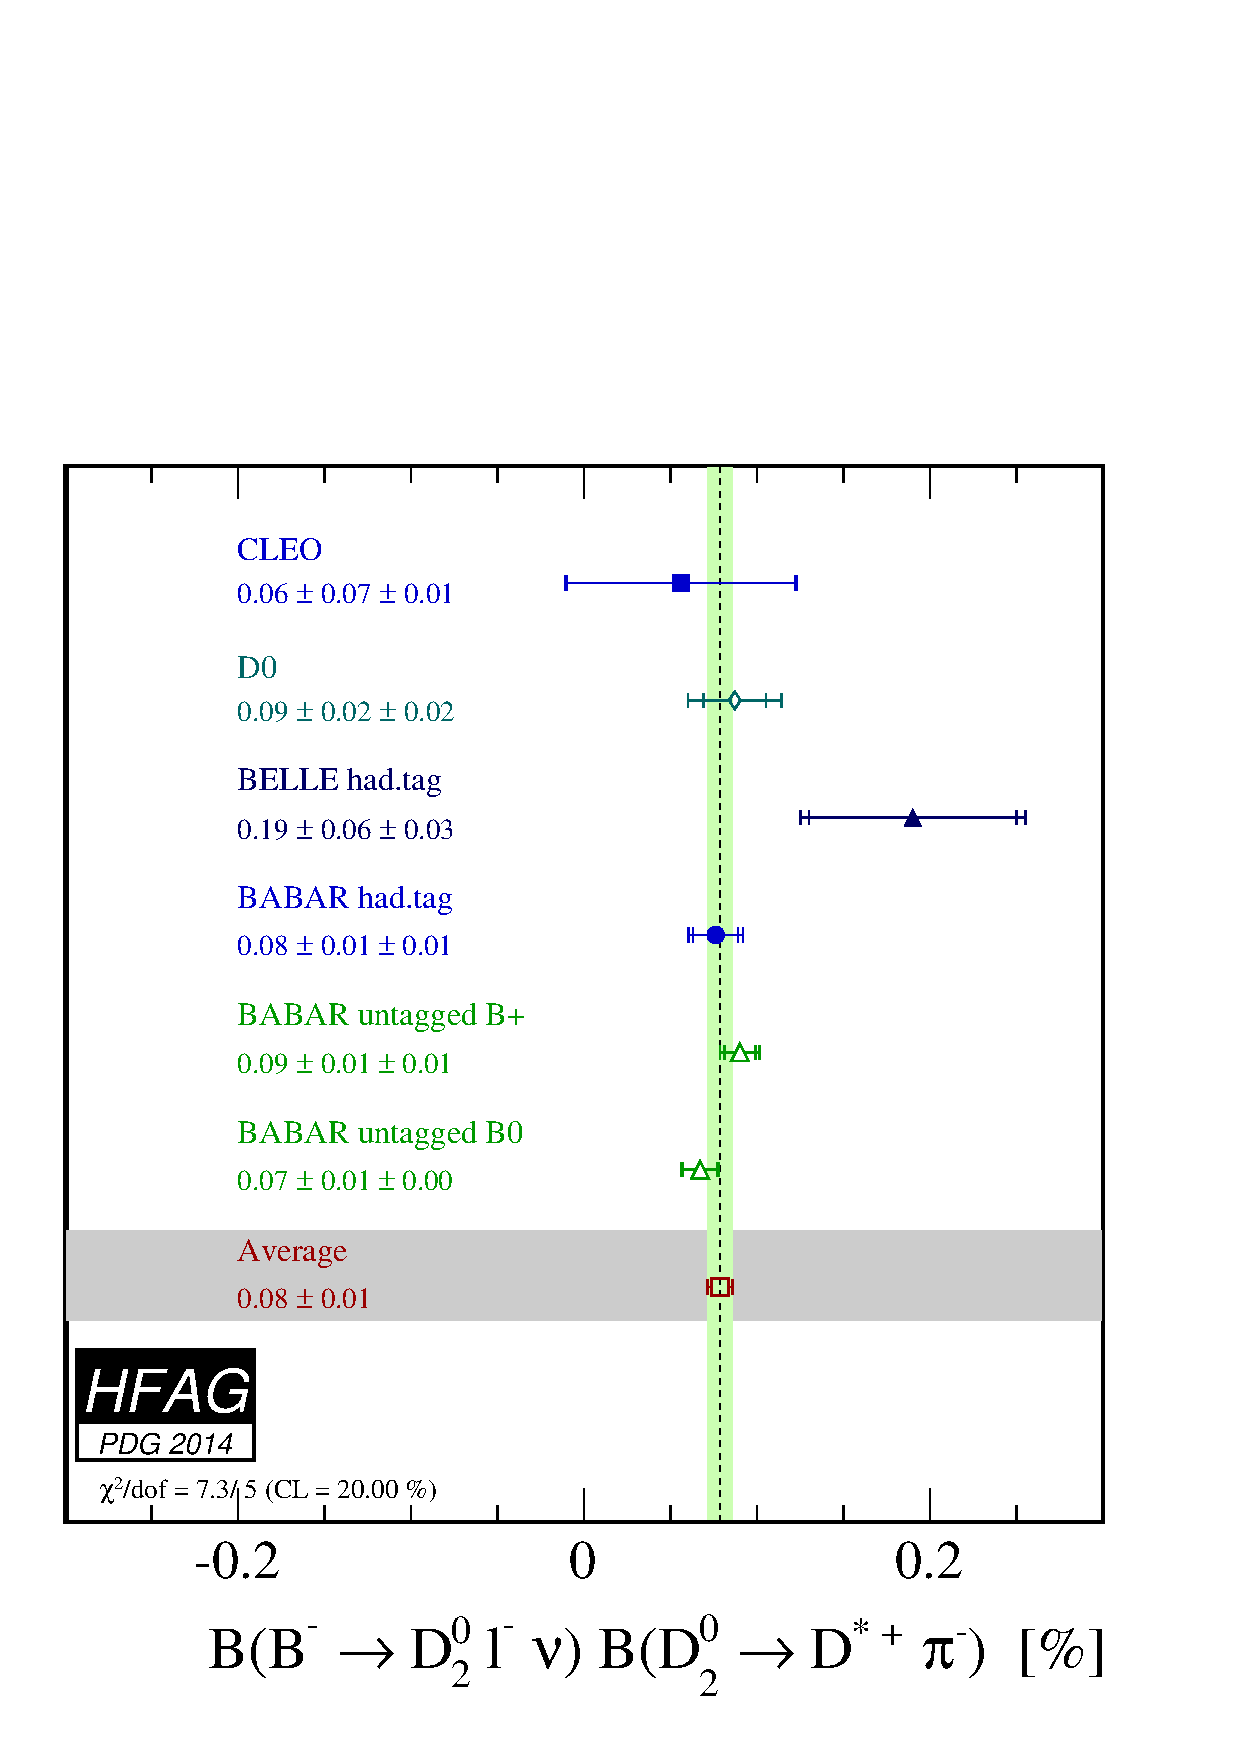
\includegraphics[width=7.55cm]{figures/slb/br_dss2l.pdf}
   }
   \put(  5.5,  7.0){{\large\bf a)}}
   \put( 14.0,  7.0){{\large\bf b)}}
  \end{picture}
  \caption{Average of the product of branching fraction (a) 
  $\cbf(B^- \to D_1^0(D^{*+}\pi^-)\ell^-\bar{\nu}_{\ell})
\times \cbf(D_1^0 \to D^{*+}\pi^-)$ and (b) $\cbf(B^- \to D_2^0(D^{*+}\pi^-)\ell^-\bar{\nu}_{\ell})
\times \cbf(D_2^0 \to D^{*+}\pi^-)$. The corresponding individual results are also shown.}
  \label{fig:brdssl}
 \end{center}
\end{figure}

\begin{figure}[!ht]
 \begin{center}
  \unitlength1.0cm % coordinates in cm
  \begin{picture}(14.,8.0)  %ys(25.,6.0)
   \put( -0.5,  0.0){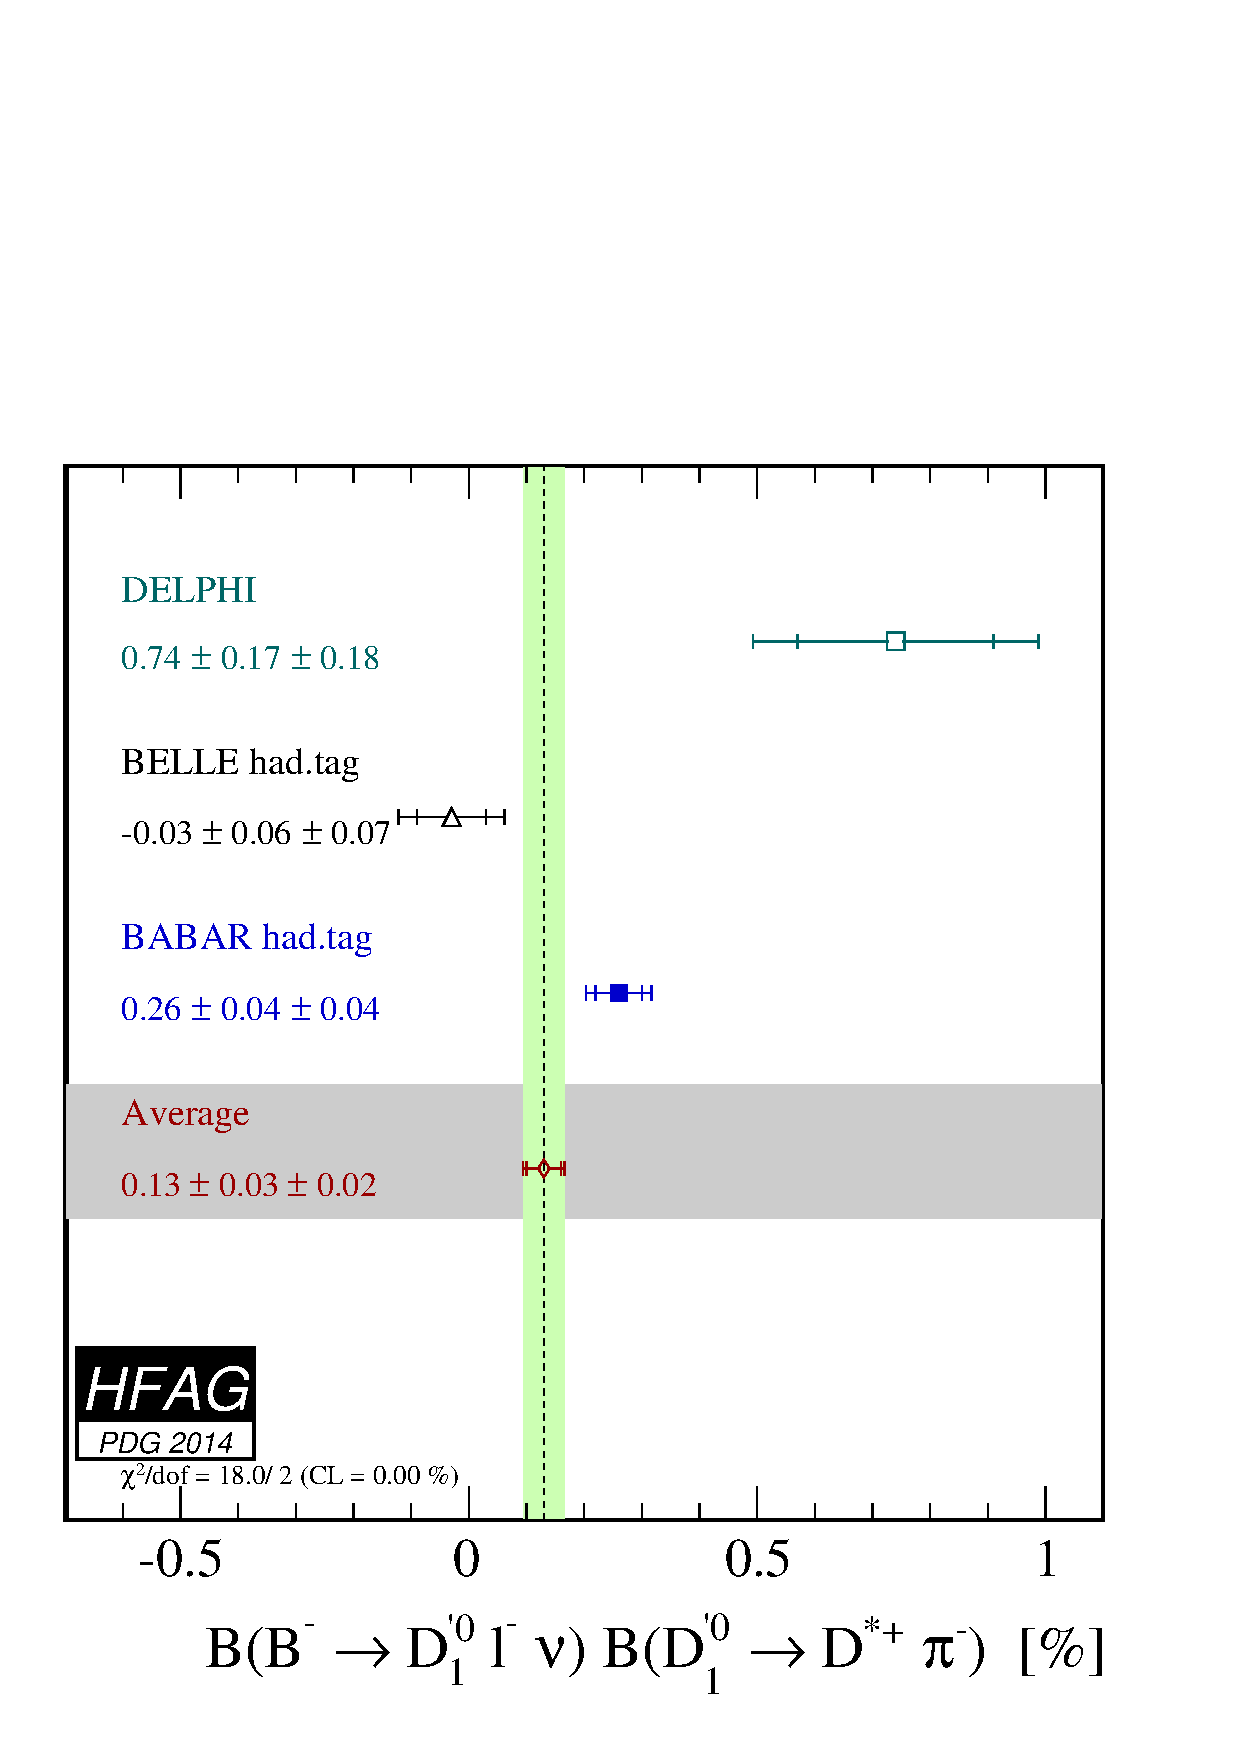
\includegraphics[width=7.8cm]{figures/slb/br_dss1primel.pdf}
   }
   \put(  8.0,  0.0){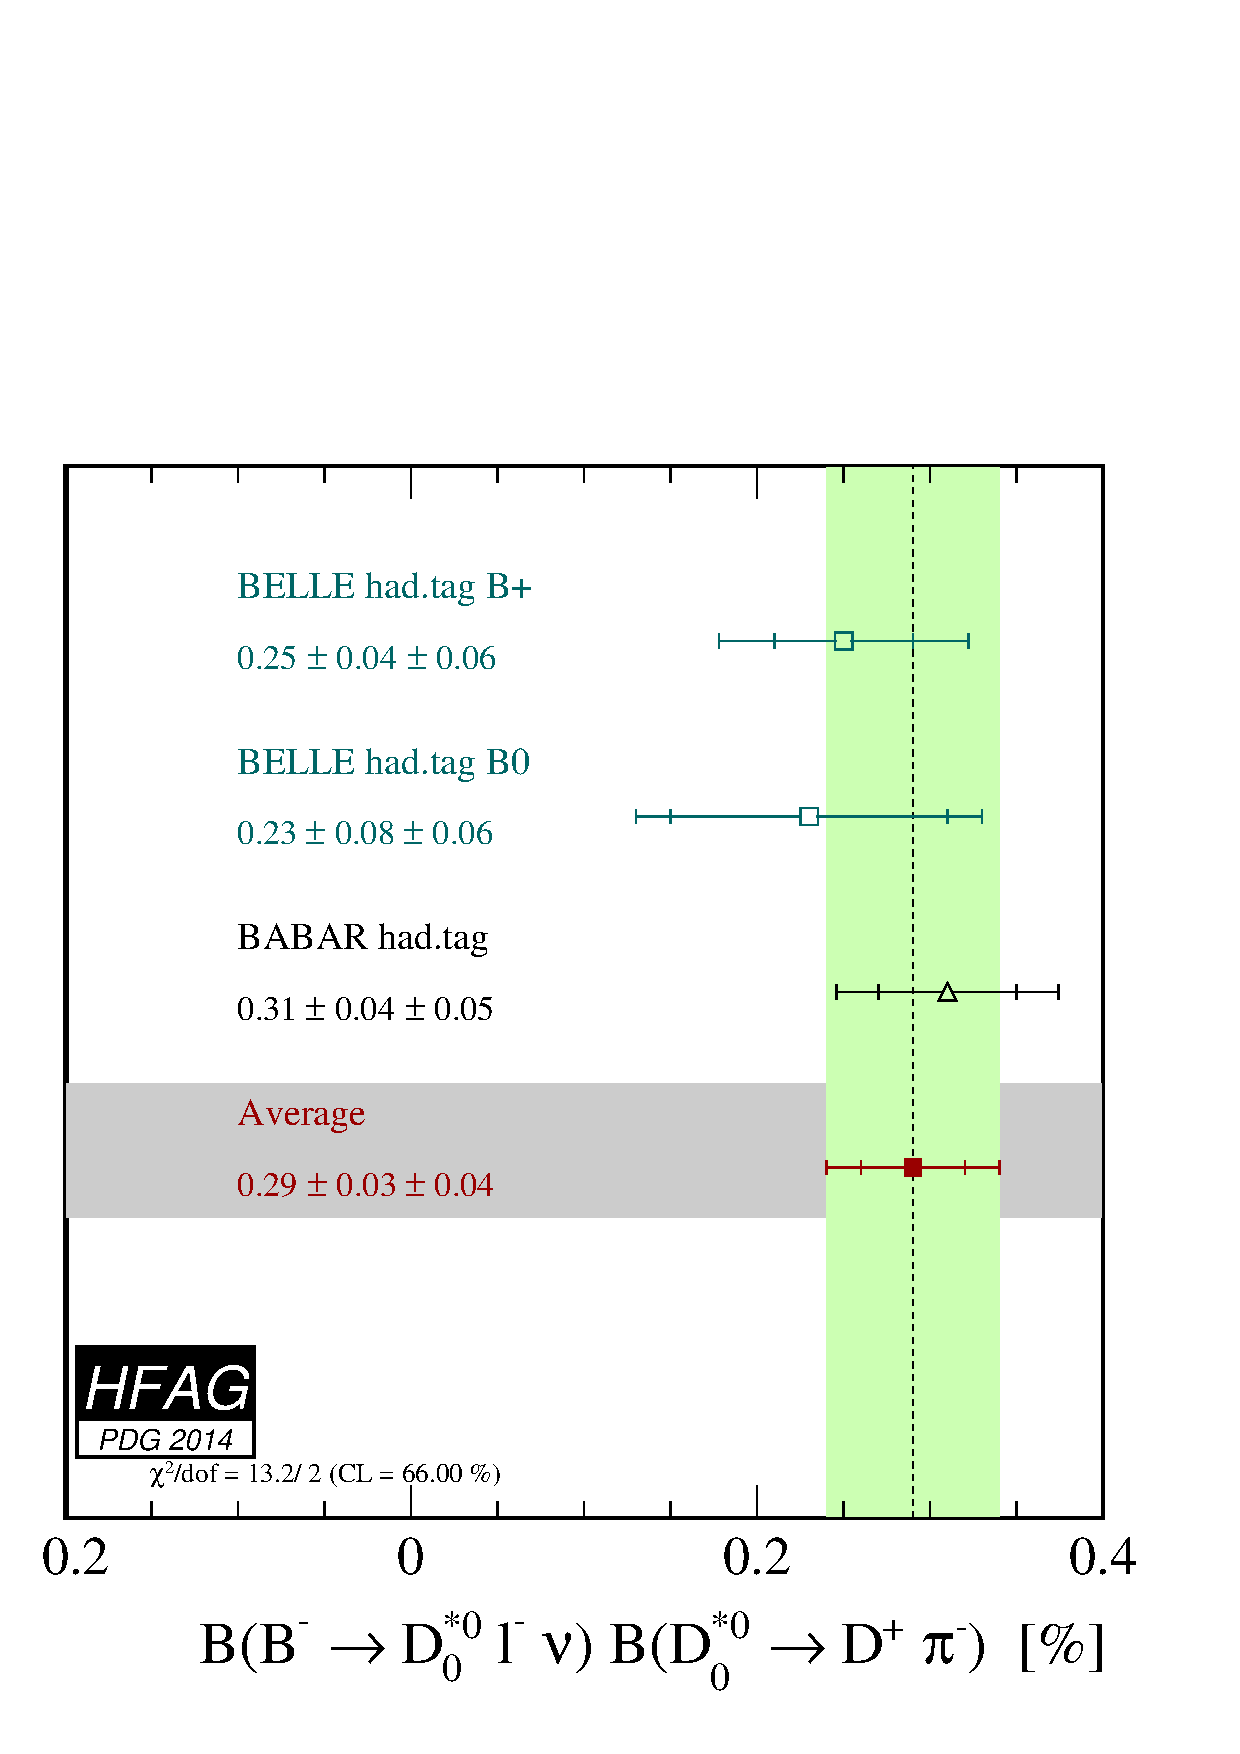
\includegraphics[width=7.8cm]{figures/slb/br_dss00l.pdf}
   }
   \put(  5.5,  7.3){{\large\bf a)}}
   \put( 14.4,  7.3){{\large\bf b)}}
  \end{picture}
  \caption{Average of the product of branching fraction (a) 
  $\cbf(B^- \to D_1'^0(D^{*+}\pi^-)\ell^-\bar{\nu}_{\ell})
\times \cbf(D_1'^0 \to D^{*+}\pi^-)$ and (b) $\cbf(B^- \to D_0^{*0}(D^{*+}\pi^-)\ell^-\bar{\nu}_{\ell})
\times \cbf(D_0^{*0} \to D^{+}\pi^-)$
The corresponding individual
  results are also shown.}
  \label{fig:brdssl2}
 \end{center}
\end{figure}


%
% ======================================================================
% Inclusive CKM-favoured decays
% -- \include{b2cincl.tex}
% ======================================================================
\subsection{Inclusive CKM-favored decays}
\label{slbdecays_b2cincl}
% -------------------------------------------

\subsubsection{Global analysis of $\bar B\to X_c\ell^-\bar\nu_\ell$}

The semileptonic width $\Gamma(\bar B\to X_c\ell^-\bar\nu_\ell)$ has
been calculated in the framework of the Operator Product
Expansion~\cite{Shifman:1986mx,*Chay:1990da,*Bigi:1992su,*Bigi:1992su_erratum}.
The result is a double-expansion in $\Lambda_{\rm QCD}/m_b$ and
$\alpha_s$, which depends on a number of non-perturbative
parameters. These parameters give information on the dynamics of the
$b$-quark inside the $B$~hadron and can be measured using other
observables in $\bar B\to X_c\ell^-\bar\nu_\ell$ decays, such as the
moments of the lepton energy and the hadronic mass spectrum.

Two independent sets of theoretical expressions, named after the
definition of the $b$-quark mass used, are available for this kind of
analysis: the kinetic~\cite{Benson:2003kp,Gambino:2004qm,Gambino:2011cq} and 1S
scheme expressions~\cite{Bauer:2004ve}. The non-perturbative
parameters in the kinetic scheme
are: the quark masses $m_b$ and $m_c$, $\mu^2_\pi$ and
$\mu^2_G$ at $O(1/m^2_b)$, and $\rho^3_D$ and $\rho^3_{LS}$ at
$O(1/m^3_b)$. In the 1S scheme, the parameters are: $m_b$, $\lambda_1$
at $O(1/m^2_b)$, and $\rho_1$, $\tau_1$, $\tau_2$ and $\tau_3$ at
$O(1/m^3_b)$. Note that due to the different definitions, the results
for the quark masses cannot be compared directly between the two
schemes.

Our analysis uses all available measurements of moments in $\bar B\to
X_c\ell^-\bar\nu_\ell$, excluding only points with too high
correlation to avoid numerical issues. The list of included
measurements is given in
Table~\ref{tab:gf_input}. The only external input is the average
lifetime~$\tau_B$ of neutral and charged $B$~mesons, taken to be
$(1.579\pm 0.005)$~ps (Sec.~\ref{sec:life_mix}).
\begin{table}[!htb]
\caption{Experimental inputs used in the global analysis of $\bar B\to
  X_c\ell^-\bar\nu_\ell$. $n$ is the order of the moment, $c$ is the
  threshold value of the lepton momentum in GeV. In total, there are
  23 measurements from \babar, 15 measurements from Belle and 12 from
  other experiments.} \label{tab:gf_input}
\begin{center}
\begin{tabular}{|l|l|l|}
  \hline
  Experiment
  & Hadron moments $\langle M^n_X\rangle$
  & Lepton moments $\langle E^n_\ell\rangle$\\
  \hline \hline
  \babar & $n=2$, $c=0.9,1.1,1.3,1.5$ & $n=0$, $c=0.6,1.2,1.5$\\
  & $n=4$, $c=0.8,1.0,1.2,1.4$ & $n=1$, $c=0.6,0.8,1.0,1.2,1.5$\\
  & $n=6$, $c=0.9,1.3$~\cite{Aubert:2009qda} & $n=2$, $c=0.6,1.0,1.5$\\
  & & $n=3$, $c=0.8,1.2$~\cite{Aubert:2009qda,Aubert:2004td}\\
  \hline
  Belle & $n=2$, $c=0.7,1.1,1.3,1.5$ & $n=0$, $c=0.6,1.4$\\
  & $n=4$, $c=0.7,0.9,1.3$~\cite{Schwanda:2006nf} & $n=1$,
  $c=1.0,1.4$\\
  & & $n=2$, $c=0.6,1.4$\\
  & & $n=3$, $c=0.8,1.2$~\cite{Urquijo:2006wd}\\
  \hline
  CDF & $n=2$, $c=0.7$ & \\
  & $n=4$, $c=0.7$~\cite{Acosta:2005qh} & \\
  \hline
  CLEO & $n=2$, $c=1.0,1.5$ & \\
  & $n=4$, $c=1.0,1.5$~\cite{Csorna:2004kp} & \\
  \hline
  DELPHI & $n=2$, $c=0.0$ & $n=1$, $c=0.0$ \\
  & $n=4$, $c=0.0$ & $n=2$, $c=0.0$ \\
  & $n=6$, $c=0.0$~\cite{Abdallah:2005cx} & $n=3$,
  $c=0.0$~\cite{Abdallah:2005cx}\\
  \hline
\end{tabular}
\end{center}
\end{table}

Both in the kinetic and 1S schemes, the moments in $\bar B\to
X_c\ell^-\bar\nu_\ell$ are not sufficient to determine the $b$-quark
mass precisely. In the kinetic scheme analysis we constrain the $c$-quark
mass (defined in the $\overline{\rm MS}$ scheme) to the value of
Ref.~\cite{Chetyrkin:2009fv},
\begin{equation}
  m_c^{\overline{\rm MS}}(3~{\rm GeV})=(0.986\pm 0.013)~{\rm GeV}~.
\end{equation}
In the 1S~scheme analysis, the $b$-quark mass is constrained with
measurements of the photon energy moments in $B\to
X_s\gamma$~\cite{Aubert:2005cua,Aubert:2006gg,Limosani:2009qg,Chen:2001fja}.

\subsubsection{Analysis in the kinetic scheme}
\label{globalfitsKinetic}

The fit relies on the calculations of the spectral moments in $\bar
B\to X_c\ell^-\bar\nu_\ell$~decays described in
Ref.~\cite{Gambino:2011cq} and closely follows the procedure of
Ref.~\cite{Gambino:2013rza}. The analysis determines $\vcb$ and the 6
non-perturbative parameters mentioned above.

The result in terms of the main parameters is
\begin{eqnarray}
  \vcb & = & (42.46\pm 0.88)\times 10^{-3}~, \\
  m_b^{\rm kin} & = & 4.541\pm 0.023~{\rm GeV}~, \\
  \mu^2_\pi & = & 0.414\pm 0.078~{\rm GeV^2}~,
\end{eqnarray}
with a $\chi^2$ of 14.6 for $50-7$ degrees of freedom. The detailed
result and the matrix of the correlation coefficients is given in
Table~\ref{tab:gf_res_mc_kin}. The fit to the lepton energy and
hadronic mass moments is shown in Figs.~\ref{fig:gf_res_kin_el} and
\ref{fig:gf_res_kin_mx}, respectively.
\begin{table}[!htb]
\caption{Fit result in the kinetic scheme, using a precise $c$-quark
  mass constraint. The error matrix of the fit contains
  experimental and theoretical contributions. In the lower part of the
  table, the correlation matrix of the parameters is
  given.} \label{tab:gf_res_mc_kin}
\begin{center}
\resizebox{0.99\textwidth}{!}{
\begin{tabular}{|l|ccccccc|}
  \hline
  & \vcb\ [10$^{-3}$] & $m_b^{\rm kin}$ [GeV] &
  $m_c^{\overline{\rm MS}}$ [GeV] & $\mu^2_\pi$ [GeV$^2$]
  & $\rho^3_D$ [GeV$^3$] & $\mu^2_G$ [GeV$^2$] & $\rho^3_{LS}$ [GeV$^3$]\\
  \hline \hline
  value & 42.46 & \phantom{$-$}4.541 & \phantom{$-$}0.987 &
  \phantom{$-$}0.414 & \phantom{$-$}0.154 & \phantom{$-$}0.340 &
  $-$0.147\\
  error & 0.88 & \phantom{$-$}0.023 &
  \phantom{$-$}0.013 & \phantom{$-$}0.078 & \phantom{$-$}0.045 &
  \phantom{$-$}0.066 & \phantom{$-$}0.098\\
  \hline
  $|V_{cb}|$ & 1.000 & $-$0.466 & $-$0.049 &
  \phantom{$-$}0.344 & \phantom{$-$}0.161 & $-$0.190 &
  \phantom{$-$}0.019\\
  $m_b^{\rm kin}$ & & \phantom{$-$}1.000 & \phantom{$-$}0.506 &
  $-$0.113 & \phantom{$-$}0.219 & \phantom{$-$}0.487 & $-$0.156\\
  $m_c^{\overline{\rm MS}}$ & & & \phantom{$-$}1.000
  & $-$0.018 & \phantom{$-$}0.020 & \phantom{$-$}0.008 & $-$0.002\\
  $\mu^2_\pi$ & & & & \phantom{$-$}1.000 & \phantom{$-$}0.610 &
  \phantom{$-$}0.001 & \phantom{$-$}0.058\\
  $\rho^3_D$ & & & & & \phantom{$-$}1.000 & $-$0.038 & $-$0.126\\
  $\mu^2_G$ & & & & & & \phantom{$-$}1.000 & $-$0.014\\
  $\rho^3_{LS}$ & & & & & & & \phantom{$-$}1.000\\
  \hline
\end{tabular}
}
\end{center}
\end{table}
\begin{figure}
\begin{center}
  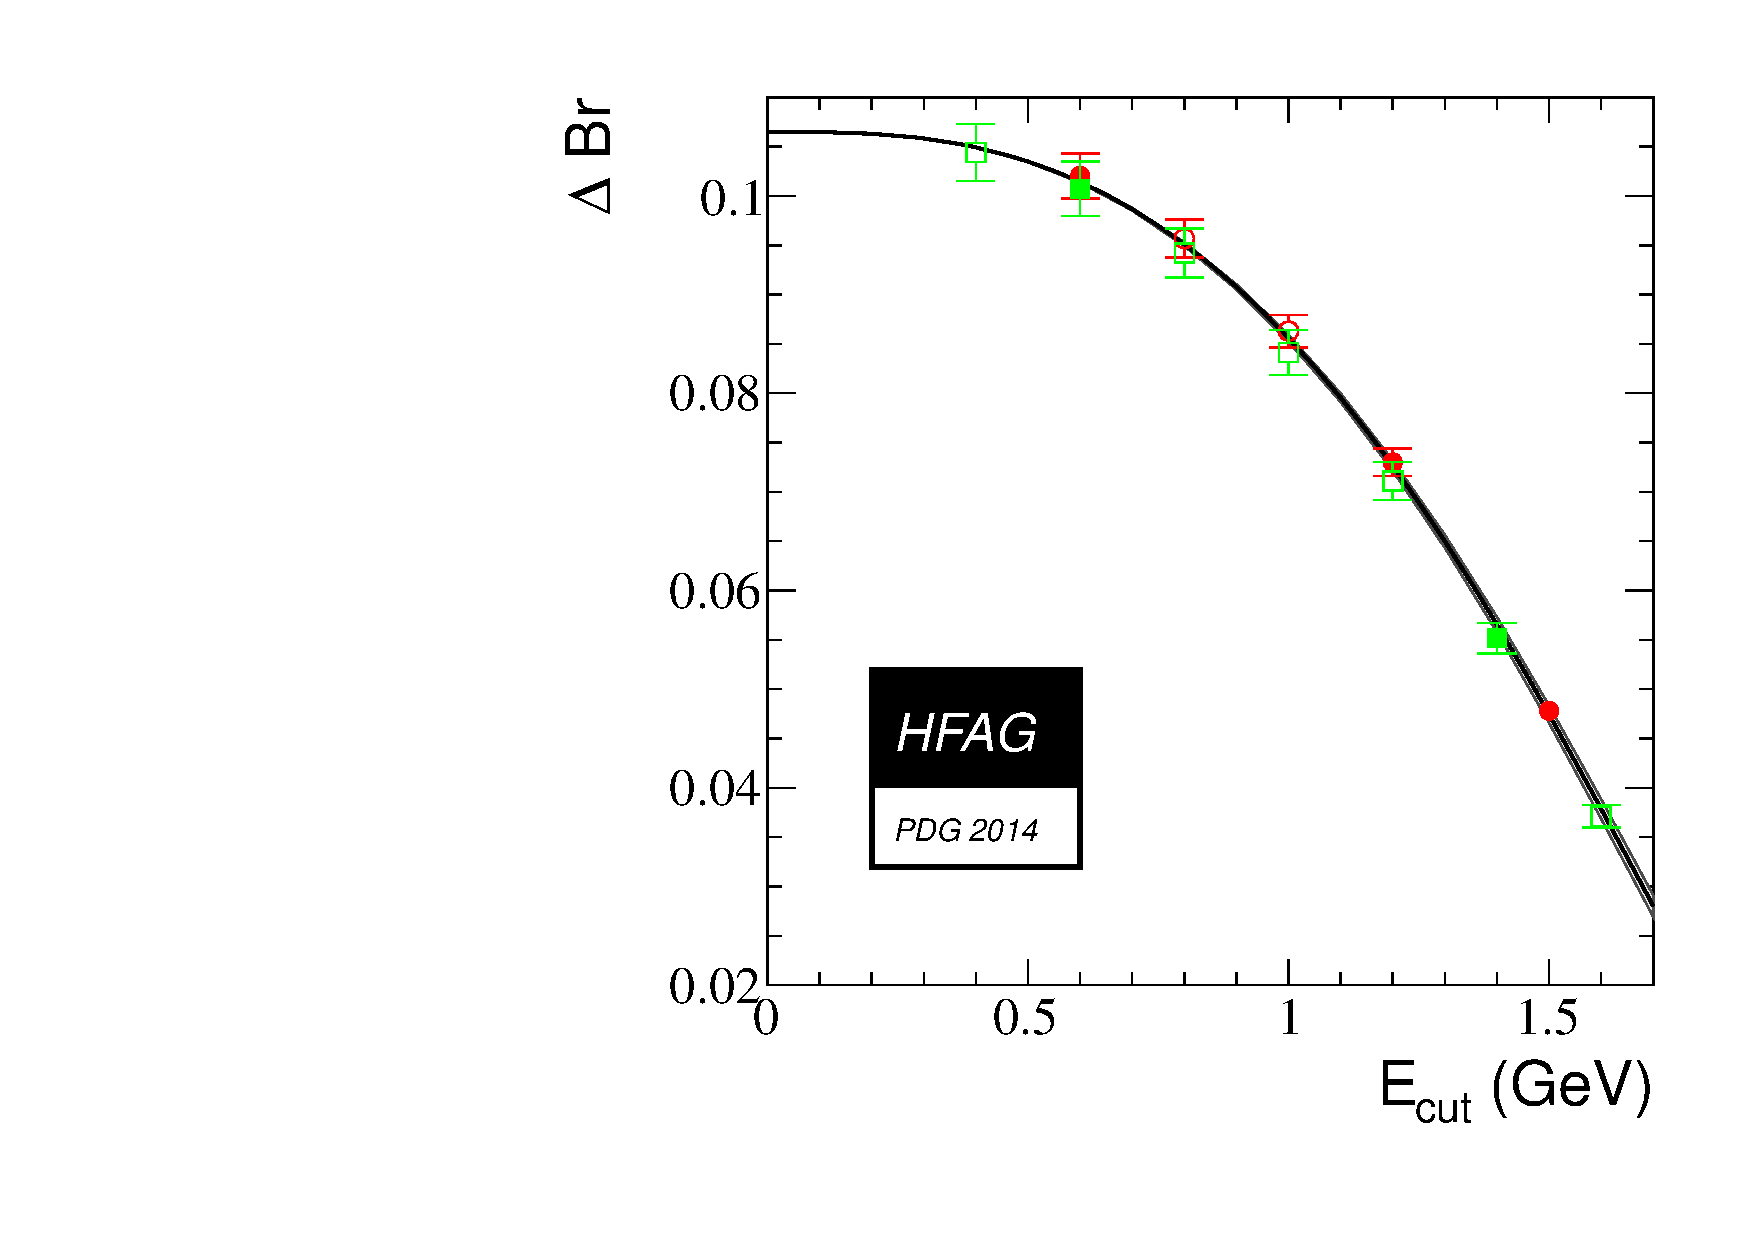
\includegraphics[width=8.2cm]{figures/slb/e0_1.pdf}
  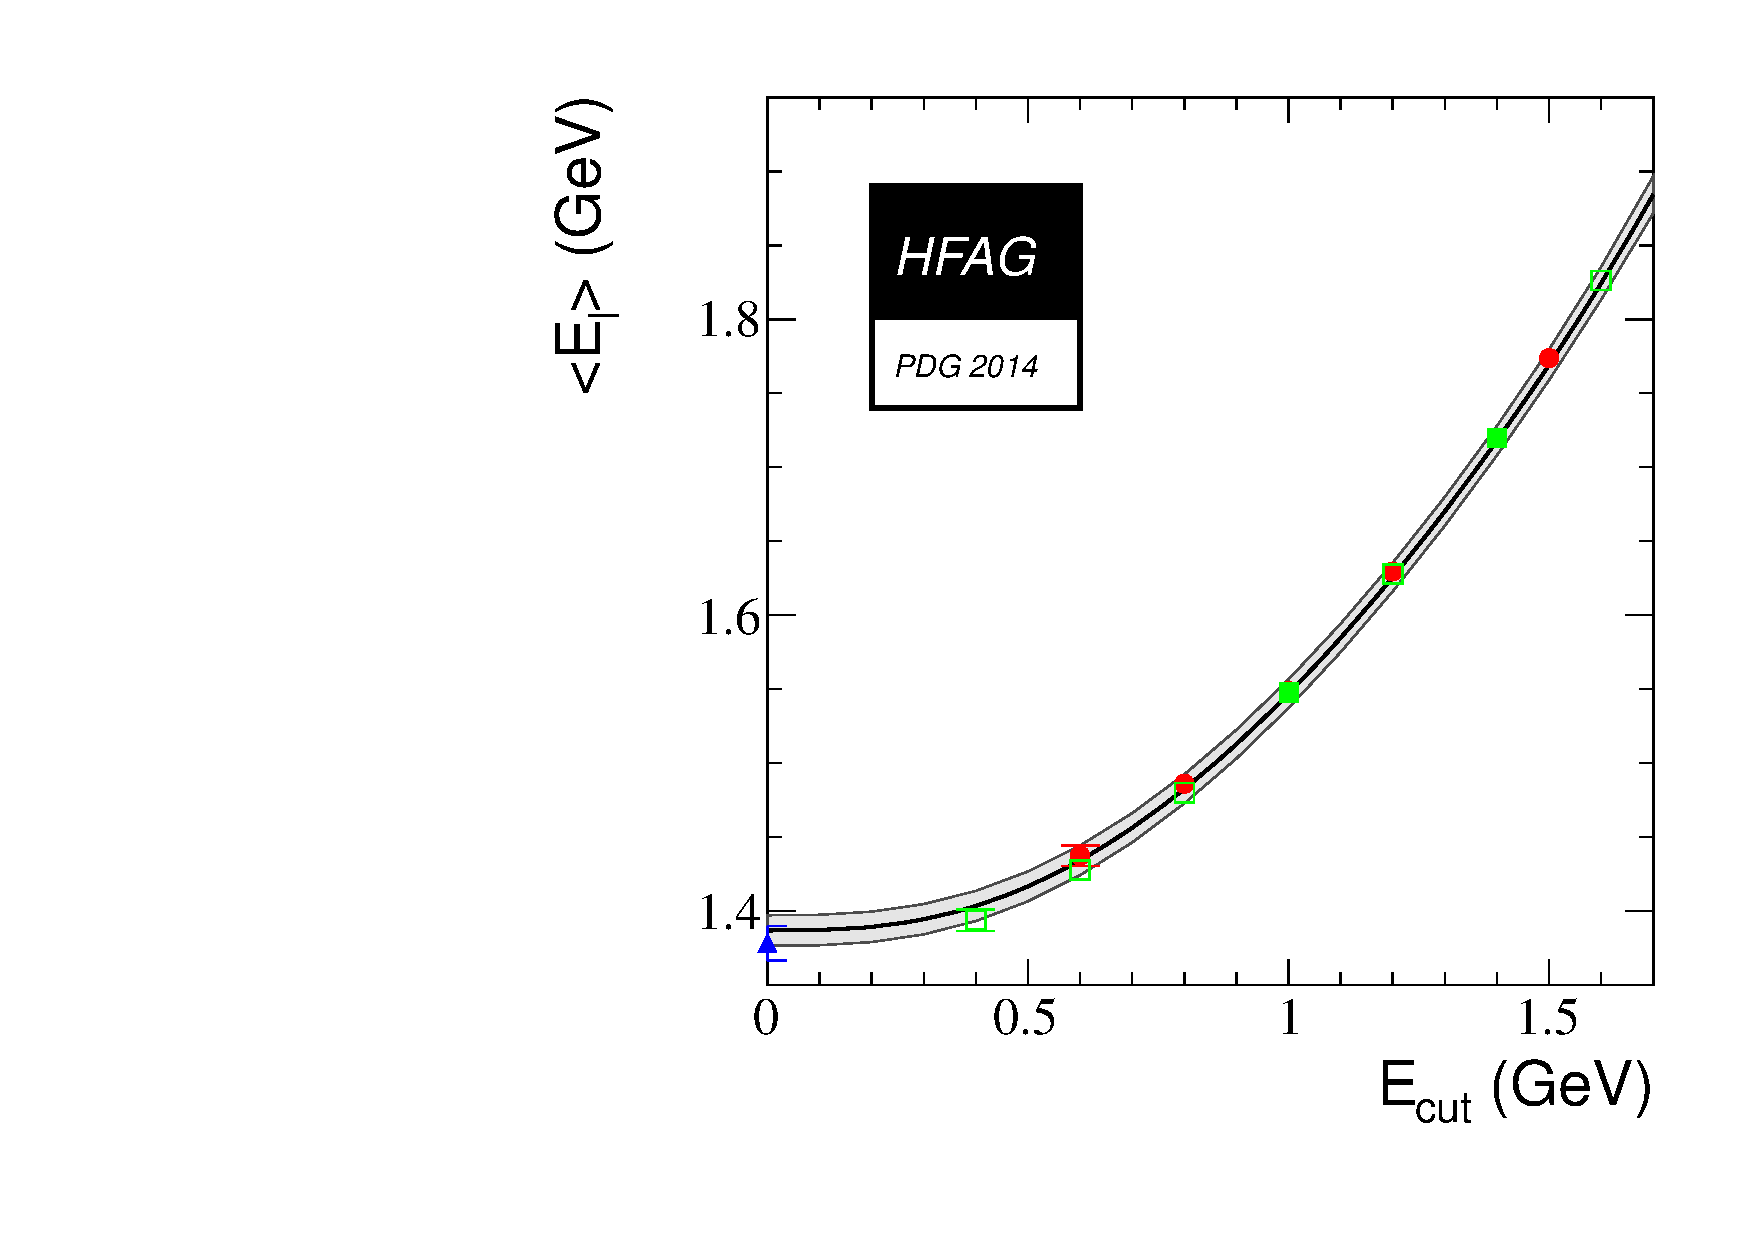
\includegraphics[width=8.2cm]{figures/slb/e1_1.pdf}\\
  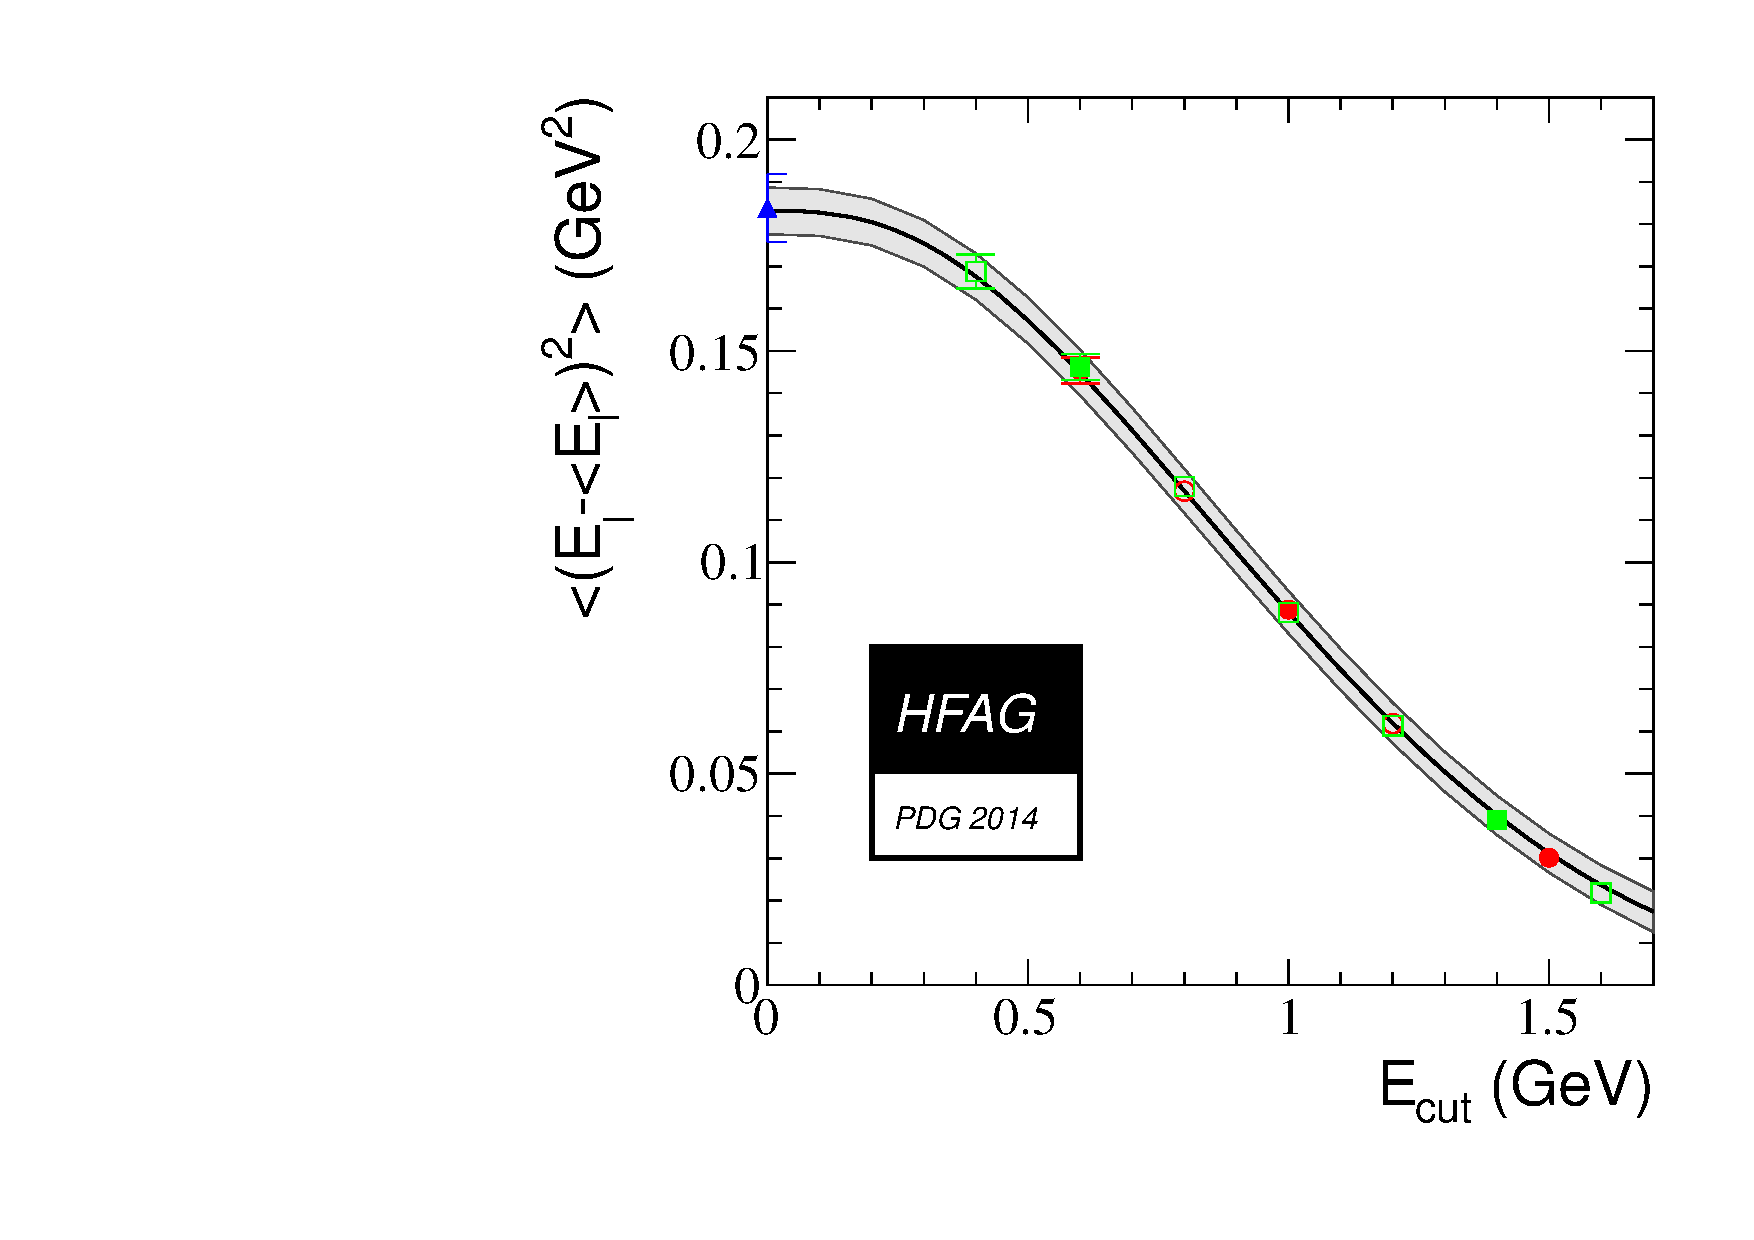
\includegraphics[width=8.2cm]{figures/slb/e2_1.pdf}
  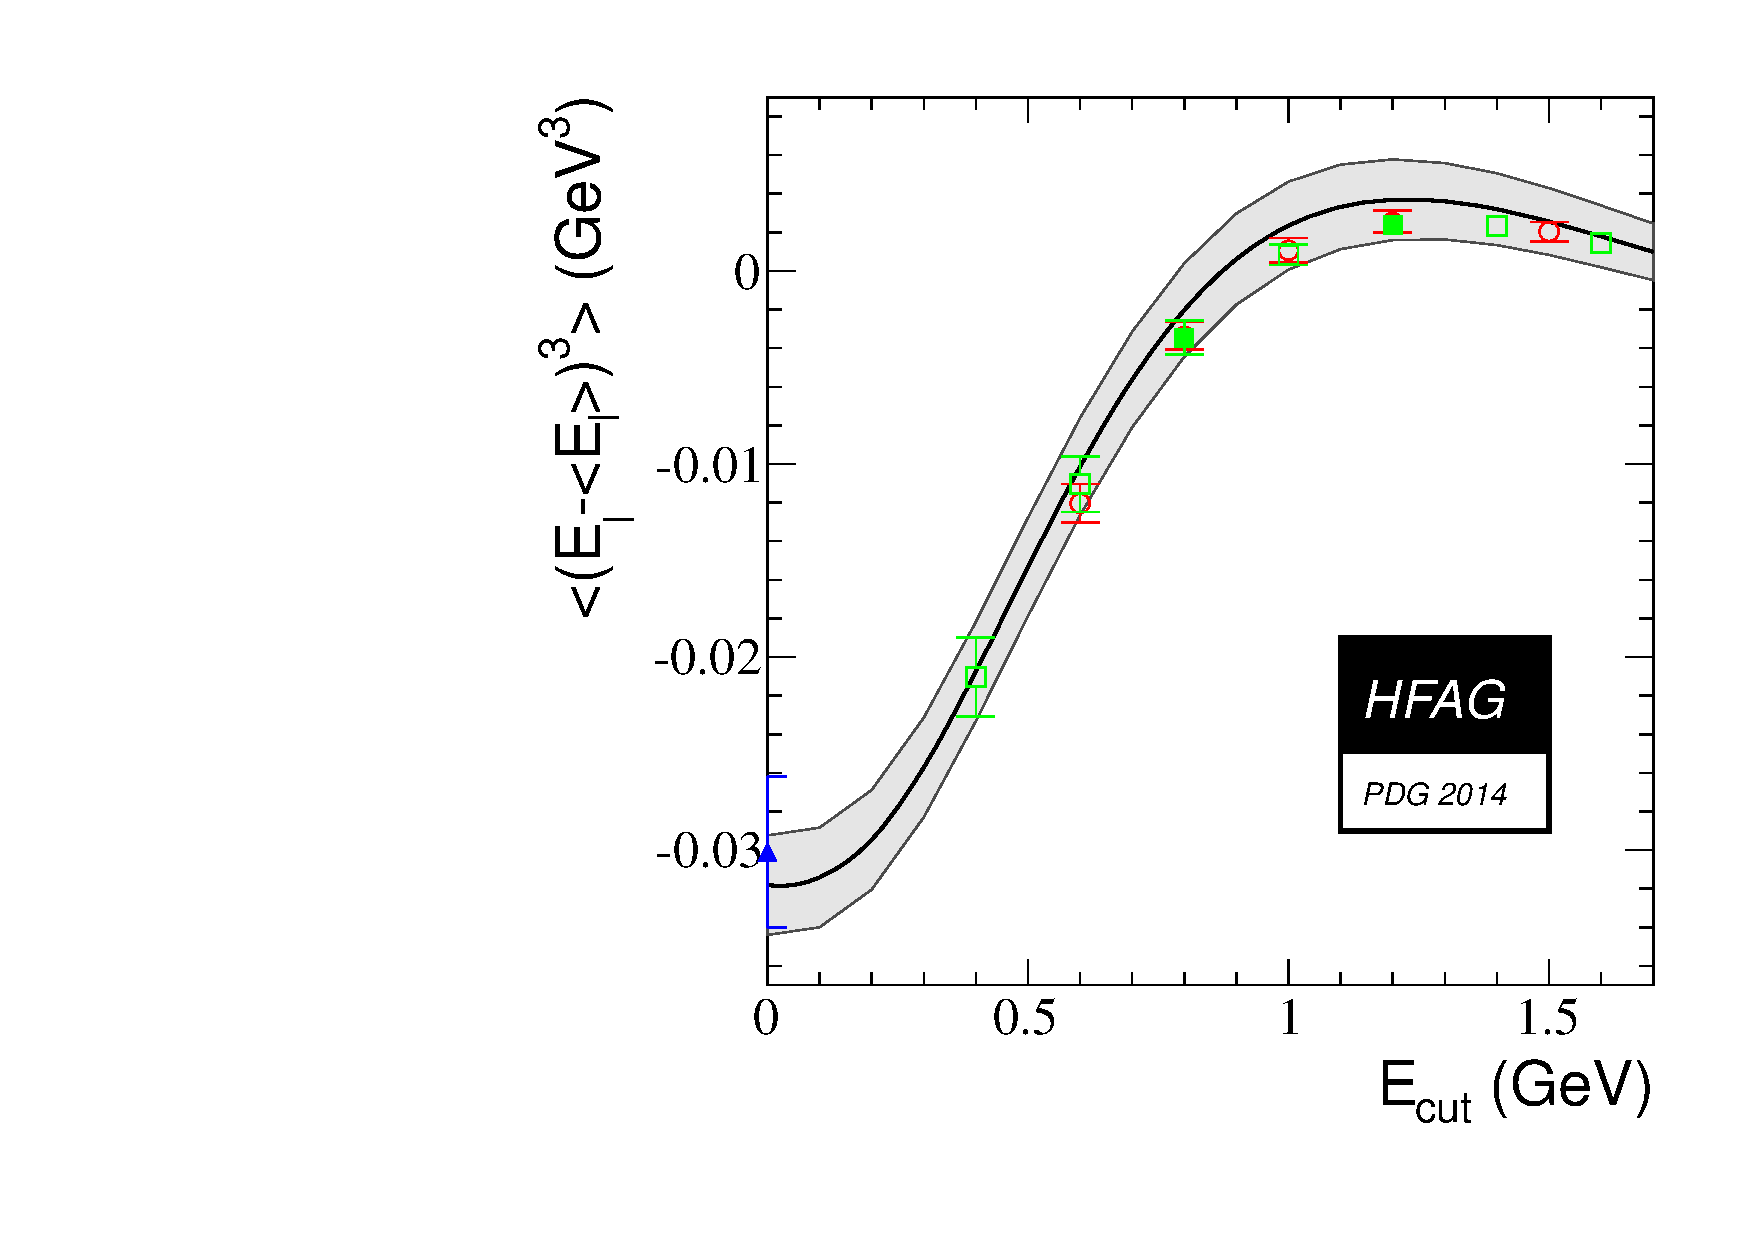
\includegraphics[width=8.2cm]{figures/slb/e3_1.pdf}
\end{center}
\caption{Fit to the partial semileptonic branching ratios and to the
  lepton energy moments in the kinetic mass scheme. In all plots, the
  grey band is the theory prediction with total theory error. \babar
  data are shown by circles, Belle by squares and other experiments
  (DELPHI, CDF, CLEO) by triangles. Filled symbols mean that the point
  was used in the fit. Open symbols are measurements that were not
  used in the fit.} \label{fig:gf_res_kin_el}
\end{figure}
\begin{figure}
\begin{center}
  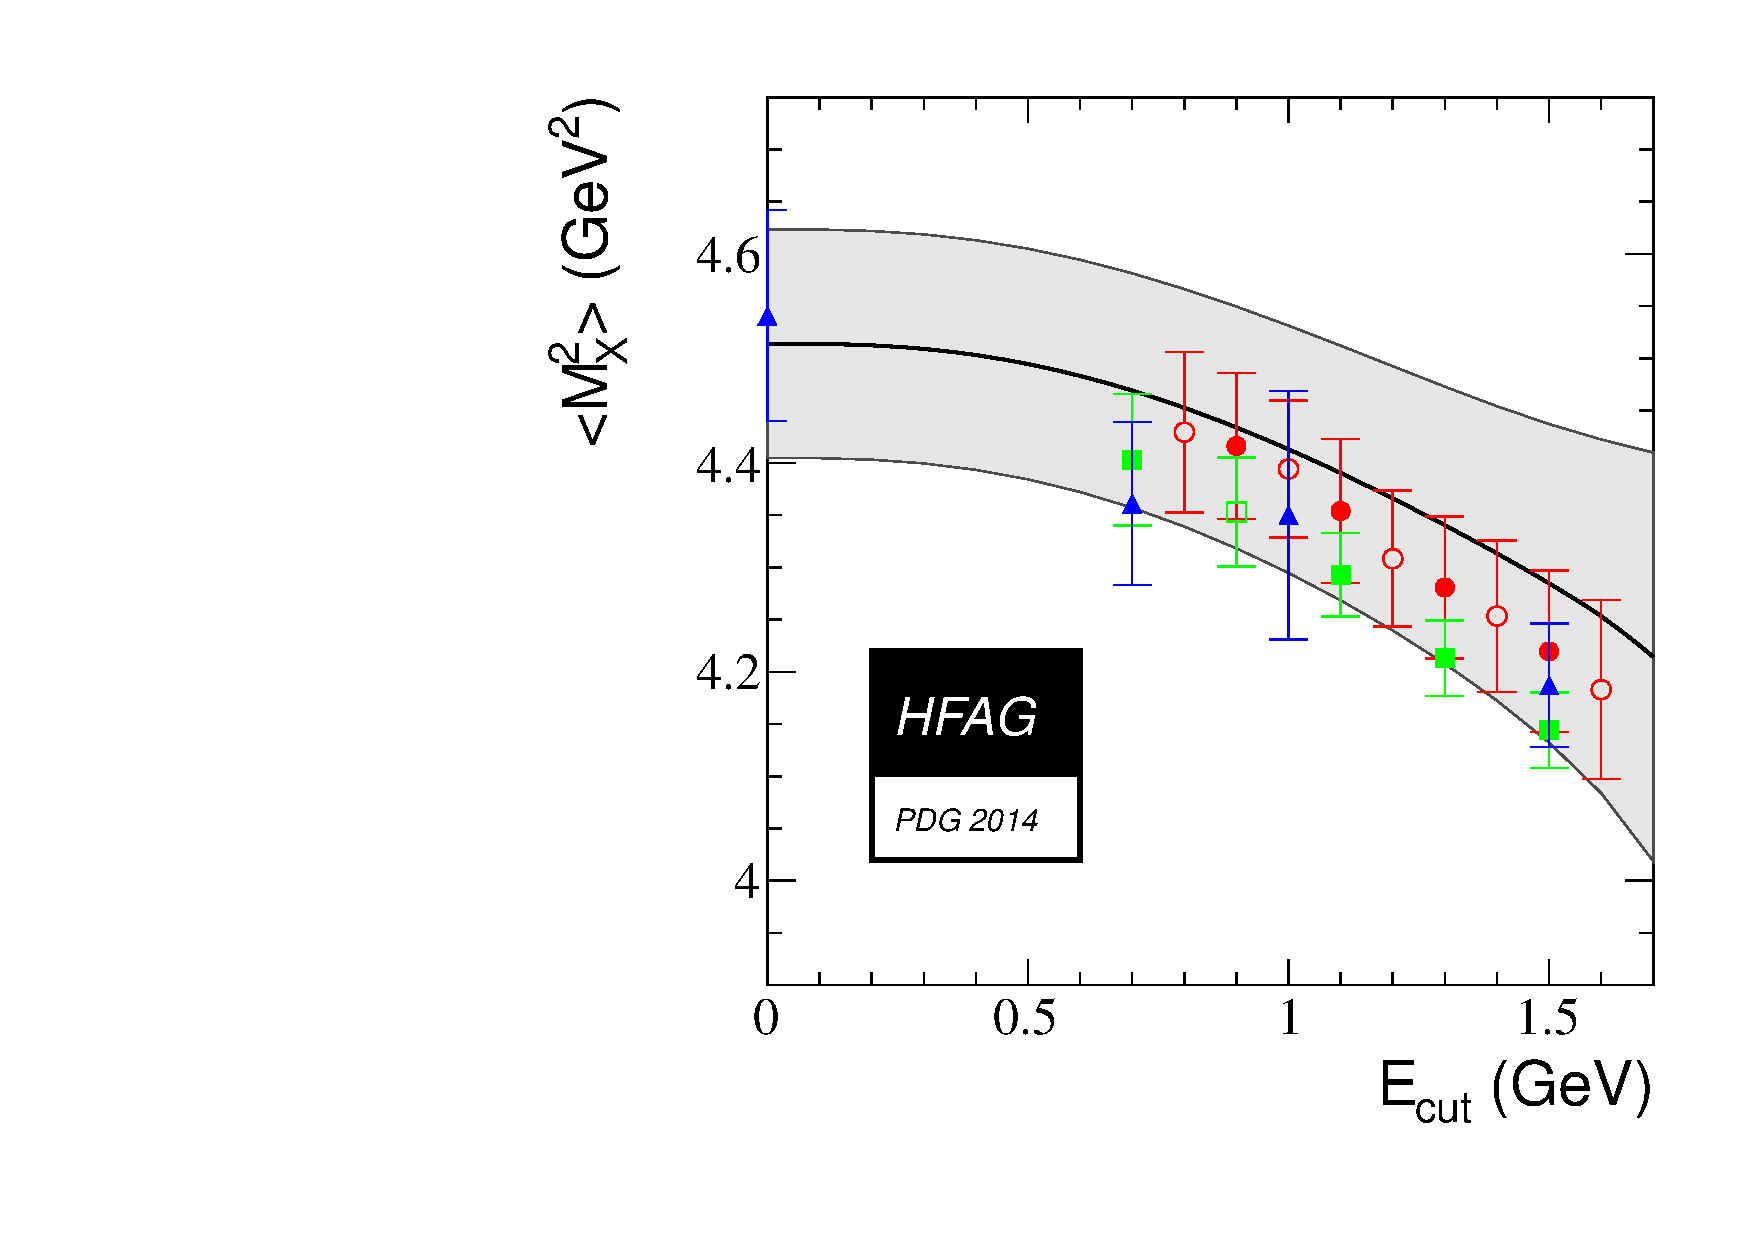
\includegraphics[width=8.2cm]{figures/slb/h1_1.pdf}
  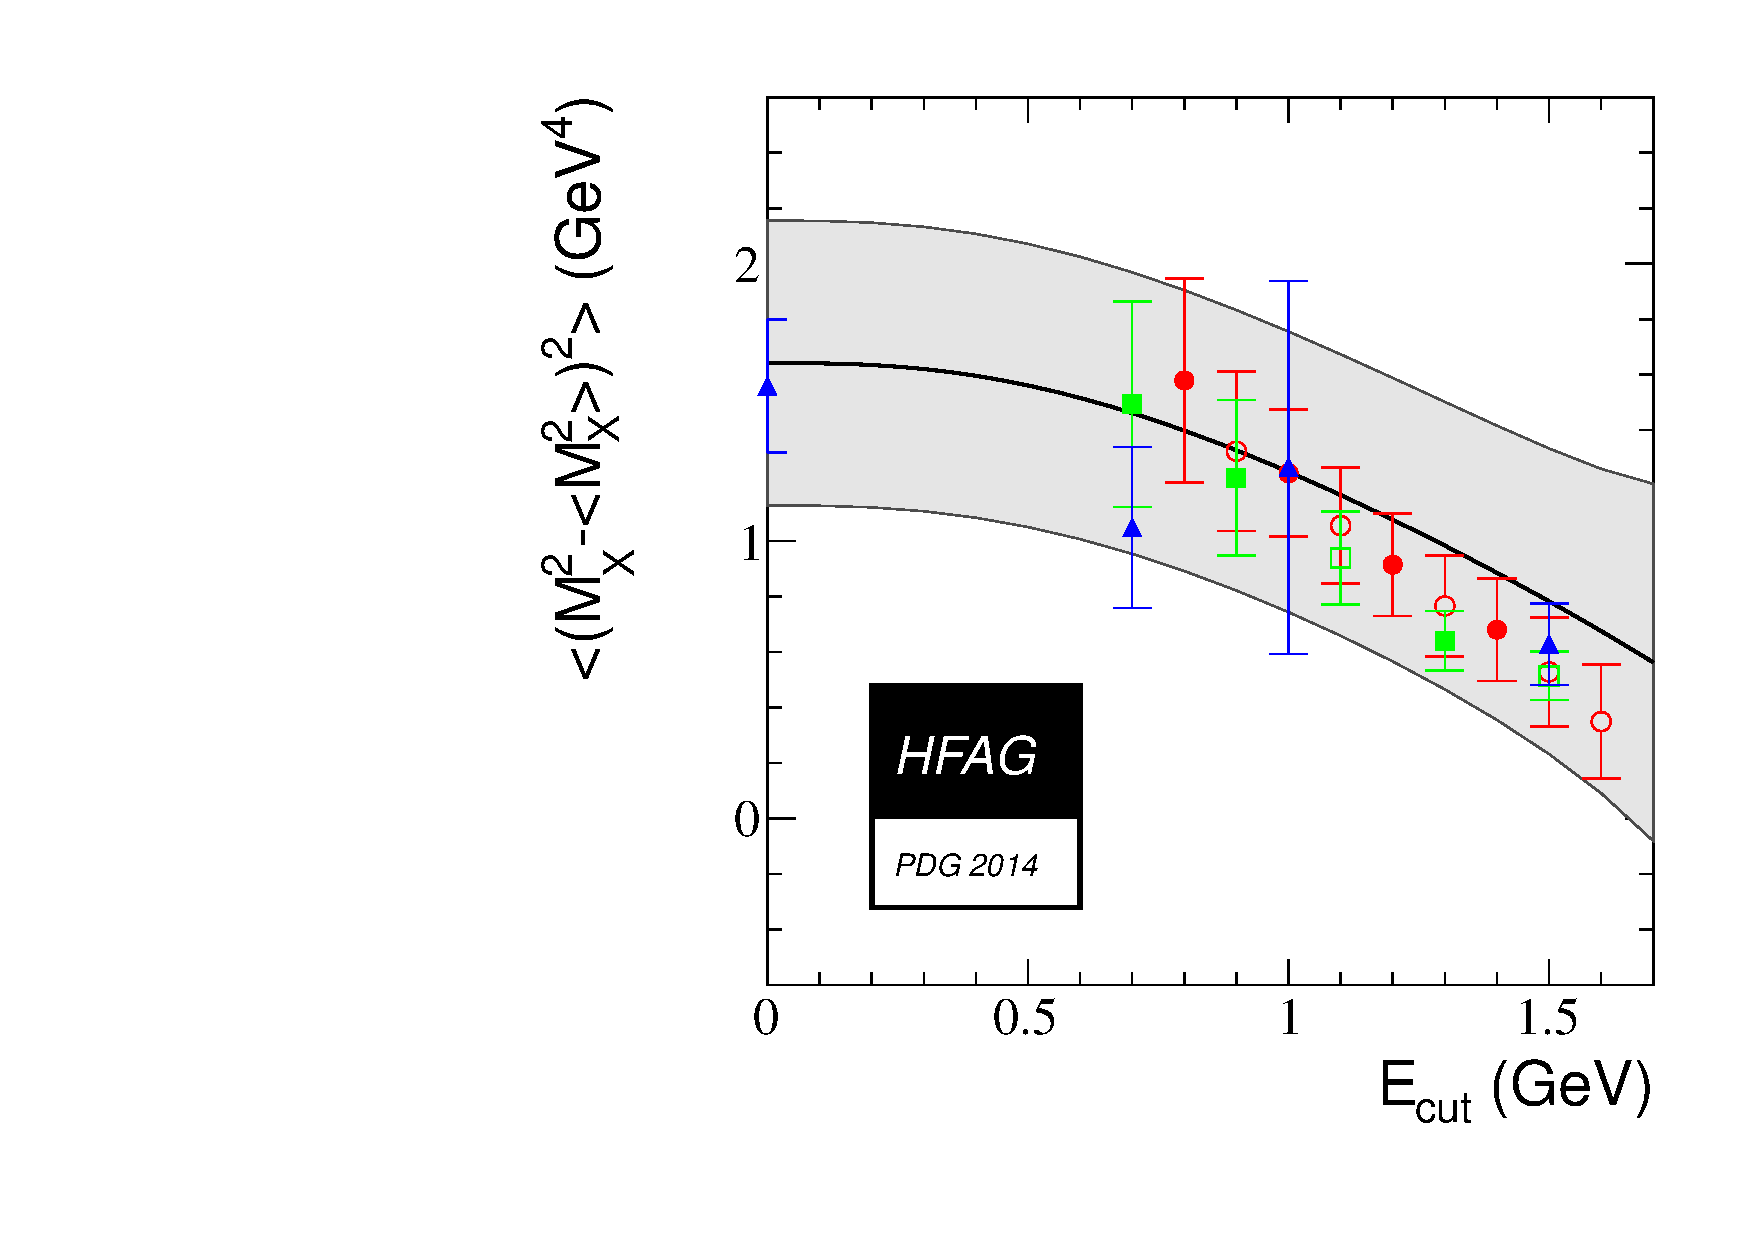
\includegraphics[width=8.2cm]{figures/slb/h2_1.pdf}\\
  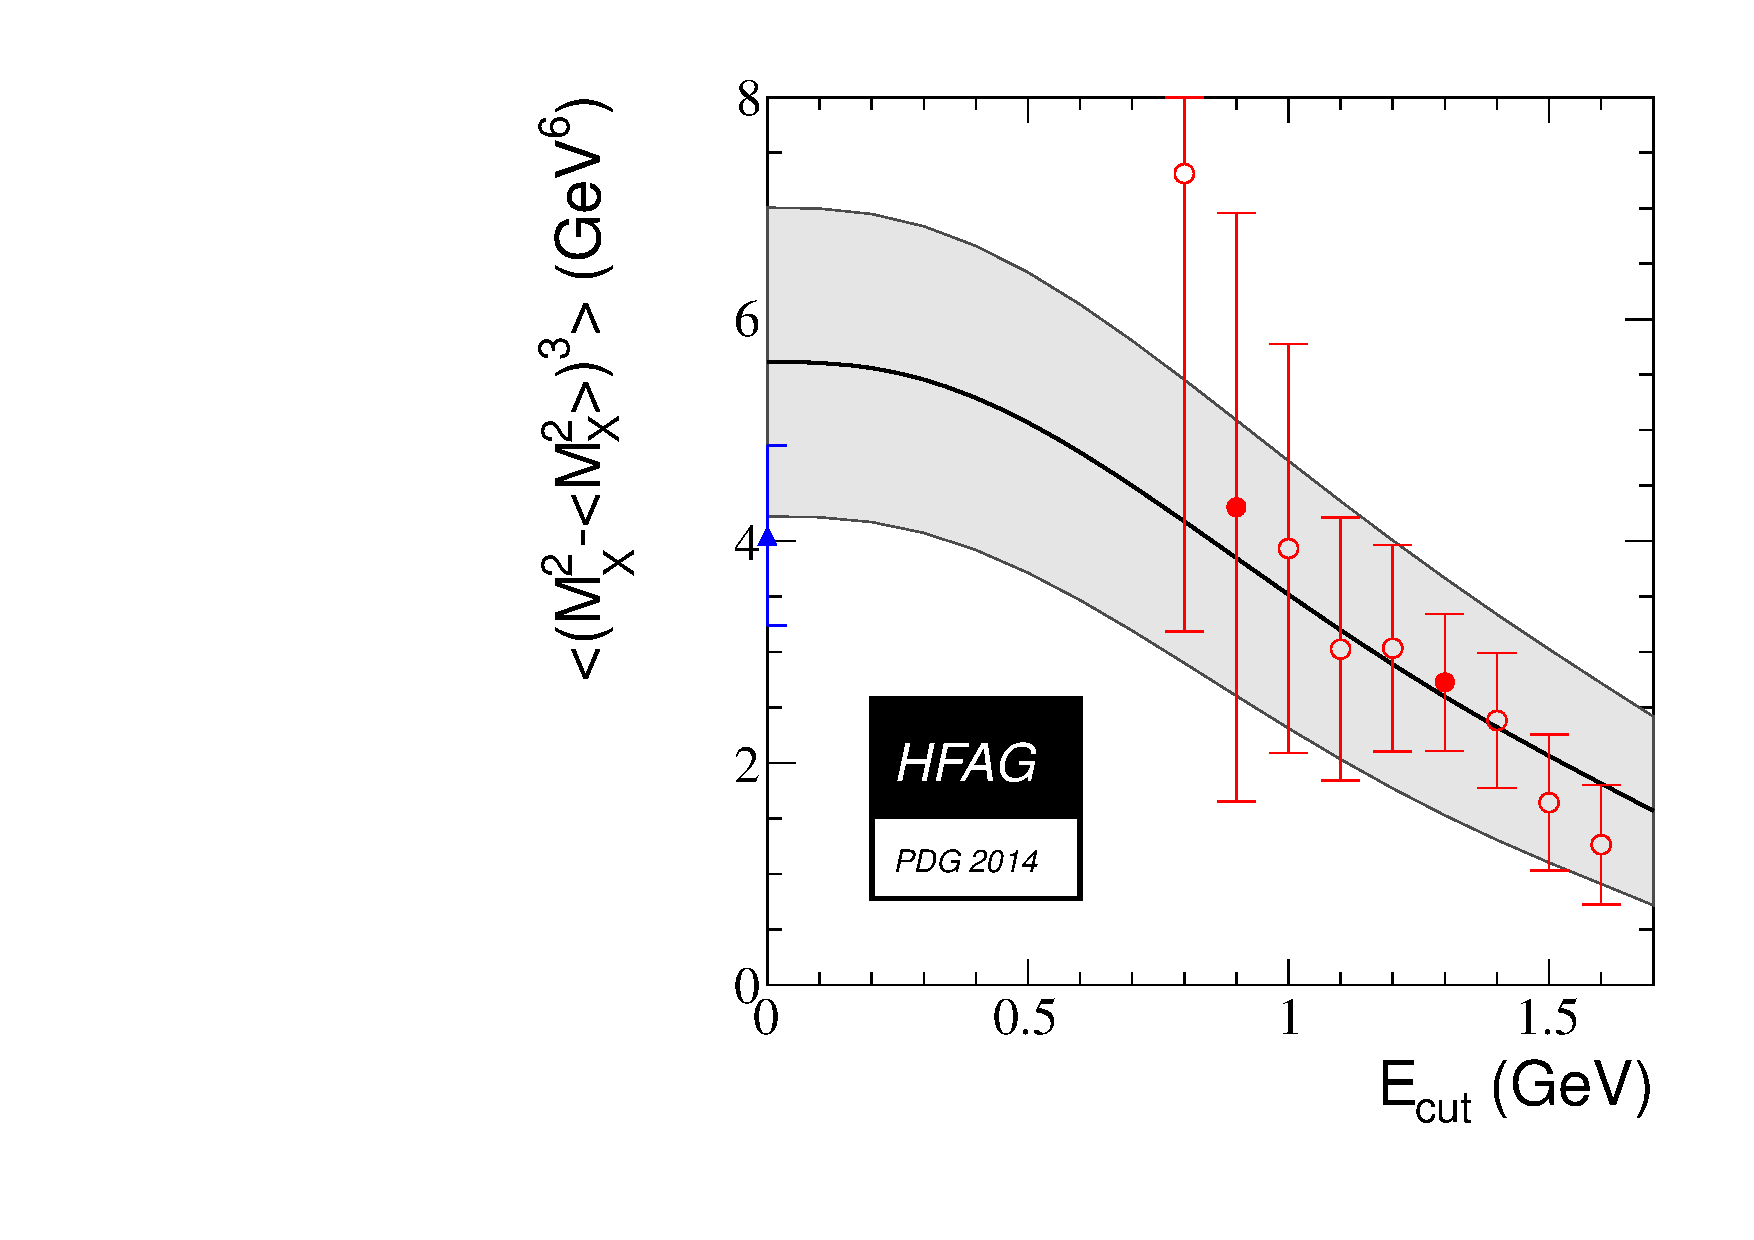
\includegraphics[width=8.2cm]{figures/slb/h3_1.pdf}
\end{center}
\caption{Same as Fig.~\ref{fig:gf_res_kin_el} for the fit to the
  hadronic mass moments in the kinetic mass
  scheme.} \label{fig:gf_res_kin_mx}
\end{figure}

The inclusive $\bar B\to X_c\ell^-\bar\nu_\ell$ branching fraction
determined by this analysis is
\begin{equation}
  \cbf(\bar B\to X_c\ell^-\bar\nu_\ell)=(10.65\pm 0.16)\%~.
\end{equation}
Correcting for charmless semileptonic decays
(Sec.~\ref{slbdecays_b2uincl}), $\cbf(\bar B\to
X_u\ell^-\bar\nu_\ell)=(2.14\pm 0.31)\times 10^{-3}$, we obtain the
semileptonic branching fraction,
\begin{equation}
  \cbf(\bar B\to X\ell^-\bar\nu_\ell)=(10.86\pm 0.16)\%~.
\end{equation}

\subsubsection{Analysis in the 1S scheme}
\label{globalfits1S}

The fit relies on the calculations of the spectral moments described in
Ref.~\cite{Bauer:2004ve}. The theoretical uncertainties are estimated
as explained in Ref.~\cite{Schwanda:2008kw}. Only trivial theory
correlations, {\it i.e.}, between the same moment at the same
threshold are included in the analysis. The fit determines $\vcb$ and
the 6 non-perturbative parameters mentioned above.

The result of the fit using the $B\to X_s\gamma$ constraint is
\begin{eqnarray}
  \vcb & = & (41.98\pm 0.45)\times 10^{-3}~, \\
  m_b^{1S} & = & 4.691\pm 0.037~{\rm GeV}~, \\
  \lambda_1 & = & -0.362\pm 0.067~{\rm GeV^2}~,
\end{eqnarray}
with a $\chi^2$ of 23.0 for $66-7$ degrees of freedom. The detailed
result of the fit is given in Table~\ref{tab:gf_res_xsgamma_1s}.
\begin{table}[!htb]
\caption{Fit result in the 1S scheme, using $B\to X_s\gamma$~moments
  as a constraint. In the lower part of the table, the correlation
  matrix of the parameters is given.} \label{tab:gf_res_xsgamma_1s}
\begin{center}
\begin{tabular}{|l|ccccccc|}
  \hline
  & $m_b^{1S}$ [GeV] & $\lambda_1$ [GeV$^2$] & $\rho_1$ [GeV$^3$] &
  $\tau_1$ [GeV$^3$] & $\tau_2$ [GeV$^3$] & $\tau_3$ [GeV$^3$] &
  $\vcb$ [10$^{-3}$]\\
  \hline \hline
  value & 4.691 & $-0.362$ & \phantom{$-$}0.043 &
  \phantom{$-$}0.161 & $-0.017$ & \phantom{$-$}0.213 &
  \phantom{$-$}41.98\\
  error & 0.037 & \phantom{$-$}0.067 & \phantom{$-$}0.048 &
  \phantom{$-$}0.122 & \phantom{$-$}0.062 & \phantom{$-$}0.102 &
  \phantom{$-$}0.45\\
  \hline
  $m_b^{1S}$ & 1.000 & \phantom{$-$}0.434 & \phantom{$-$}0.213 &
  $-0.058$ & $-0.629$ & $-0.019$ & $-0.215$\\
  $\lambda_1$ & & \phantom{$-$}1.000 & $-0.467$ & $-0.602$ & $-0.239$
  & $-0.547$ & $-0.403$\\
  $\rho_1$ & & & \phantom{$-$}1.000 & \phantom{$-$}0.129 & $-0.624$ &
  \phantom{$-$}0.494 & \phantom{$-$}0.286\\
  $\tau_1$ & & & & \phantom{$-$}1.000 & \phantom{$-$}0.062 & $-0.148$ &
  \phantom{$-$}0.194\\
  $\tau_2$ & & & & & \phantom{$-$}1.000 & $-0.009$ & $-0.145$\\
  $\tau_3$ & & & & & & \phantom{$-$}1.000 & \phantom{$-$}0.376\\
  $\vcb$ & & & & & & & \phantom{$-$}1.000\\
  \hline
\end{tabular}
\end{center}
\end{table}



% ======================================================================
% Exclusive CKM-suppressed decays
% ======================================================================
\subsection{Exclusive CKM-suppressed decays}
\label{slbdecays_b2uexcl}
% ----------------------------------------------
In this section, we list results on exclusive charmless semileptonic branching fractions
and determinations of $\vub$ based on $\Bb\to\pi\ell\nub$ decays.
The measurements are based on two different event selections: tagged
events, in which case the second $B$ meson in the event is fully
reconstructed in either a hadronic decay (``had. tag'') or in a 
CKM-favored semileptonic decay (``sl. tag''); and untagged events, in which case the momentum
of the undetected neutrino is inferred from measurements of the total 
momentum sum of the detected particles and the knowledge of the initial state.
We also present averages for $\Bb\to\rho\ell\nub$, $\Bb\to\omega\ell\nub$, $\Bb\to\eta\ell\nub$ and
$\Bb\to\eta'\ell\nub$.

The results for the full and partial branching fractions for $\Bb\to\pi\ell\nub$ are given
in Table~\ref{tab:pilnubf} and shown in Figure~\ref{fig:xlnu}.   

When averaging these results, systematic uncertainties due to external
inputs, e.g., form factor shapes and background estimates from the
modeling of $\Bb\to X_c\ell\nub$ and $\Bb\to X_u\ell\nub$ decays, are
treated as fully correlated (in the sense of Eq.~\ref{eq:correlrho}).
Uncertainties due to experimental reconstruction effects are treated
as fully correlated among measurements from a given experiment. Varying
the assumed dependence of the quoted errors on the measured value
for error sources where the dependence was not obvious had no significant impact.

\input{tables/slb/pilnubf.tex}

\begin{figure}[!ht]
 \begin{center}
  \unitlength1.0cm % coordinates in cm
  \begin{picture}(14.,8.0)  %ys(25.,6.)
  % \put(  8.0,  0.0){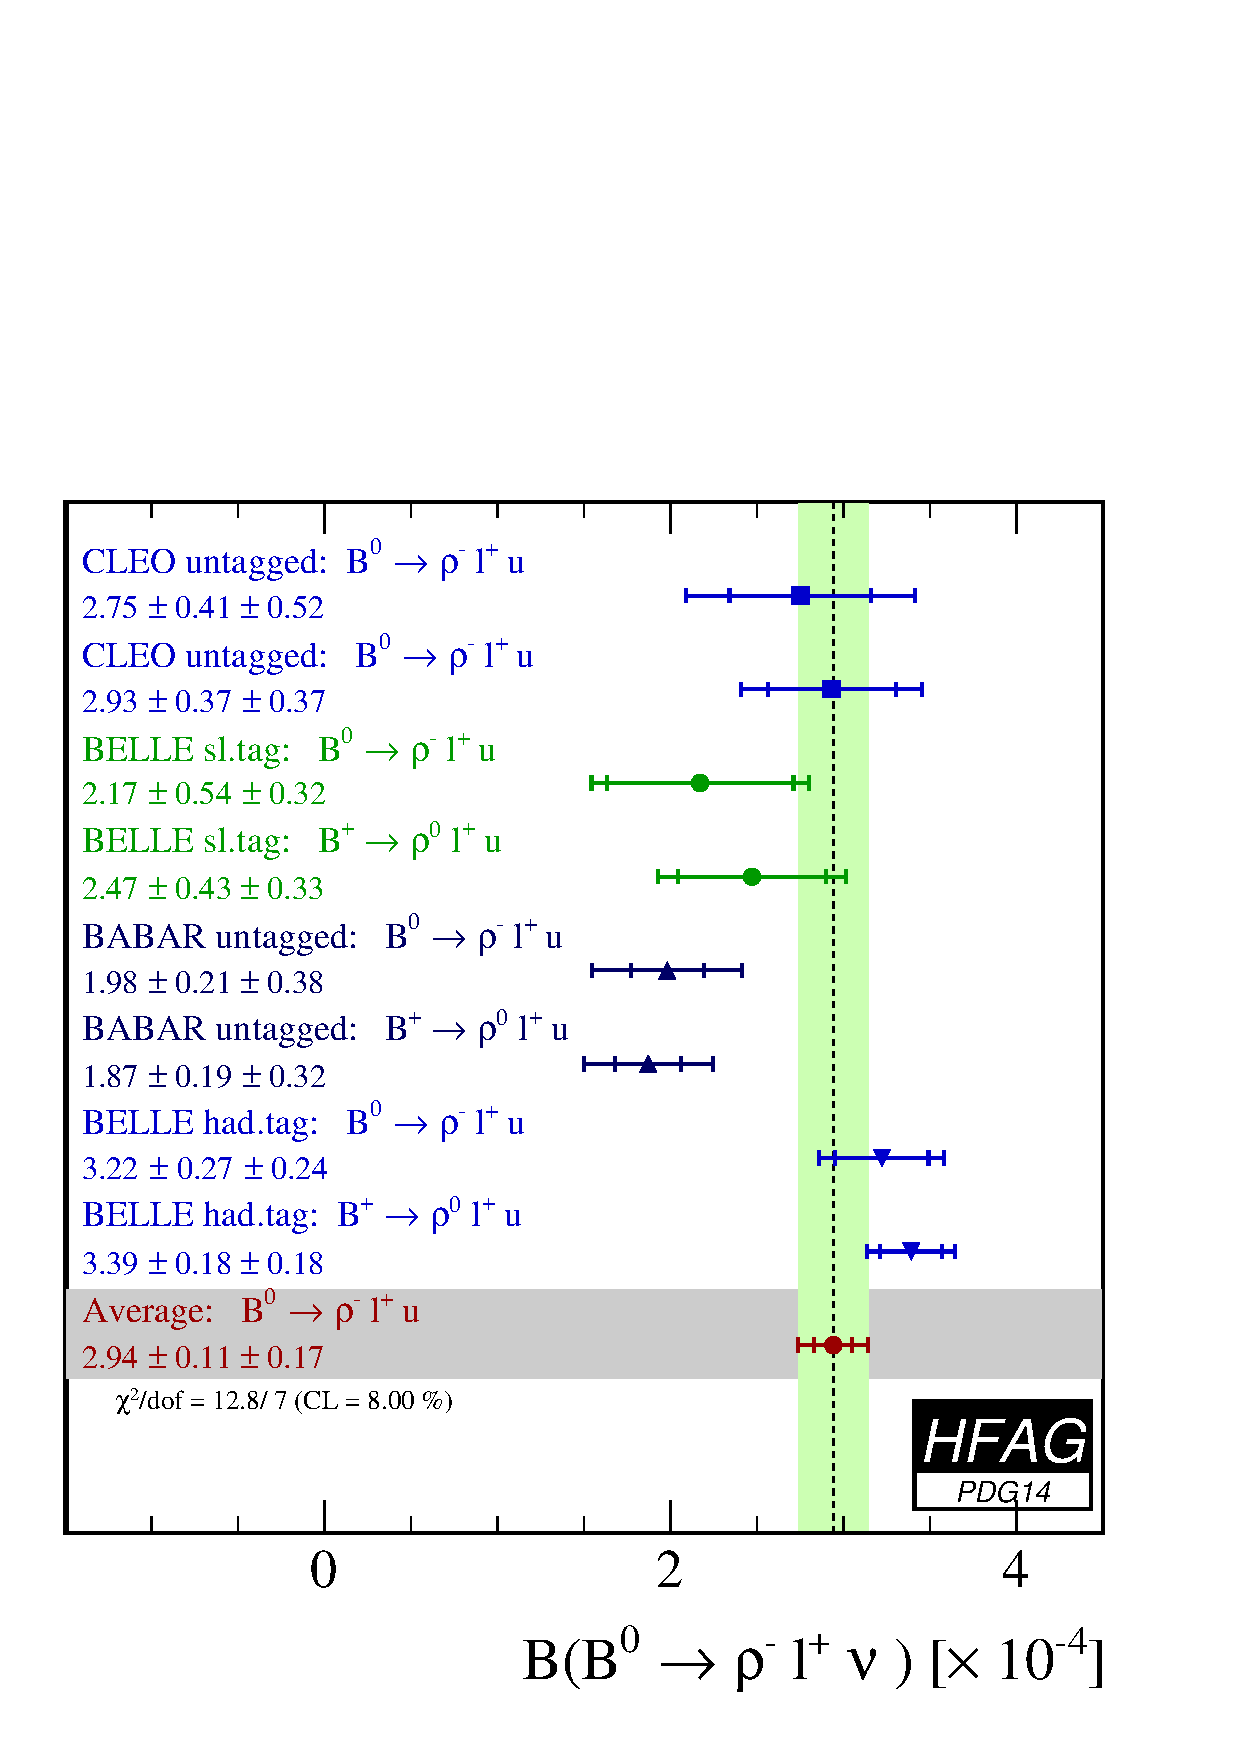
\includegraphics[width=8.0cm]{figures/slb/rholnu.pdf}}
   \put( 2.0,  0.0){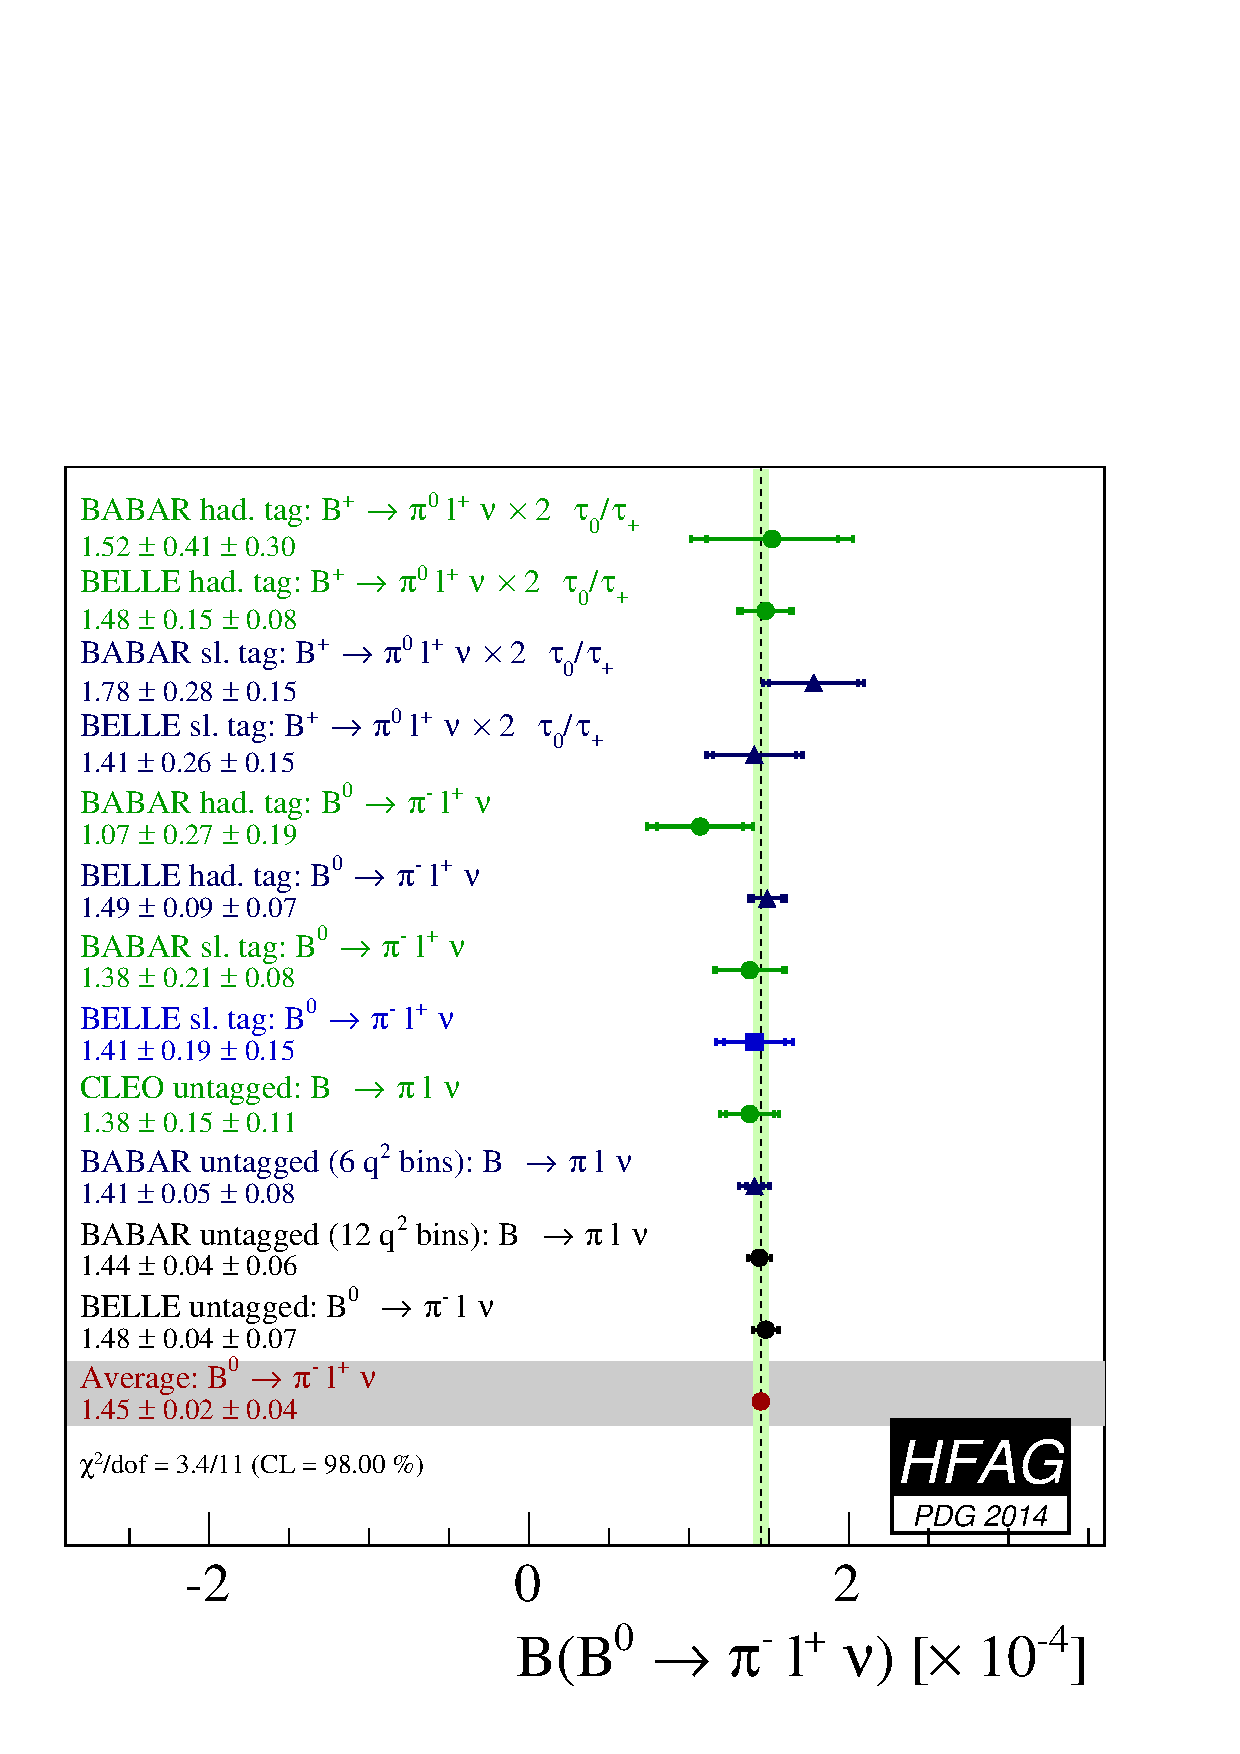
\includegraphics[width=8.8cm]{figures/slb/pilnu.pdf}
   }
 %  \put(  5.5,  7.3){{\large\bf a)}}  
 %  \put( 14.4,  7.3){{\large\bf b)}}
   \end{picture} \caption{
Summary of exclusive determinations of $\cbf(\Bb\to\pi\ell\nub)$ and their average.
Measured branching fractions for $B^+ \rightarrow \pi^0 l^+ \nu$ have been
multiplied by $2\times \tau_{B^0}/\tau_{B^+}$ in accordance with
isospin symmetry. The labels ``had. tag'' and ``sl. tag''
refer to the type of $B$ tag used in the measurement; ``untagged'' refers to an untagged measurement.
The results from the untagged measurements by CLEO and \babar are based on a combined analysis of
$B^0 \rightarrow \pi^- l^+ \nu$  and $B^+ \rightarrow \pi^0 l^+ \nu$ decays using isospin relations. 
%(b) Summary of exclusive determinations of $\cbf(\Bb\to\rho\ell\nub)$ and their average.
}
\label{fig:xlnu}
\end{center}
\end{figure}

The determination of \vub\ from $\Bb\to\pi\ell\nub$ decays is
shown in Table~\ref{tab:pilnuvub}, and uses our averages for the partial branching
fractions given in Table~\ref{tab:pilnubf}, combined with various form factor calculations. 
Two theoretical approaches are used: unquenched lattice QCD (LQCD) and QCD light-cone sum rules (LCSR).
Lattice calculations of the form factors are limited to small hadron momenta, i.e.
large $q^2$, while calculations based on light-cone sum rules are restricted
to small $q^2$. 

\input{tables/slb/pilnuvub.tex}

An alternative method to determine \vub\ from $\Bb\to\pi\ell\nub$ decays that makes use
of the measurement over the full $q^2$ range is based on a simultaneous fit of a
$B\to \pi$ form factor parameterization to data and theory predictions. 
We choose the BCL (Bourrely, Caprini, Lellouch) parameterization~\cite{Bourrely:2008za} up to order $z^2$.
There are 3+1 fit parameters: the three coefficients of the BCL power series ($b_0$, $b_1$, $b_2$)
and \Vub, which is determined from the relative normalization between data and theory predications. 
As the shape of the $q^2$ spectrum is determined by only two parameters ($b_1$ and $b_2$), we quote
the ratios $b_1/b_0$ and $b_2/b_0$ as results for the shape determined in the fit.

The result of the simultaneous fit to the four most precise measurements from \babar and Belle 
(\babar untagged 6 $q^2$ bins, \babar untagged 12 $q^2$ bins, Belle untagged, Belle had. tag)
and the FNAL/MILC LQCD calculations is shown in Figure~\ref{fig:vub_pilnu_simultaneous}~(a). 
The fit probability is 0.053 ($\chi^2/dof = 60.2/44$) and we obtain the following values:
\begin{eqnarray}
\Vub &=& (3.28 \pm 0.29) \times 10^{-3}, \\
b_1/b_0 &=& -1.02 \pm 0.18, \\
b_2/b_0 &=& -1.20 \pm 0.57.
\end{eqnarray}
The fit results correspond to a value of the product $f_+(0)\Vub$ of $(0.923 \pm 0.024) \times 10^{-3}$. 
The correlation matrix of the fit parameters is:
\begin{center}
\begin{tabular}{ccccc}
      & $b_0$ & $b_1$ & $b_2$ & \Vub  \\
$b_0$ & 1.00  & -0.54 &  0.15 & -0.29 \\
$b_1$ &       &  1.00 & -0.89 &  0.24 \\ 
$b_2$ &       &       &  1.00 & -0.14 \\  
\Vub  &       &       &       &  1.00 \\
\end{tabular}
\end{center}

\begin{figure}[!ht]
 \begin{center}
  \unitlength1.0cm % coordinates in cm

  \begin{picture}(14.,8.0)  %ys(25.,6.)
   \put( -0.5,  0.0){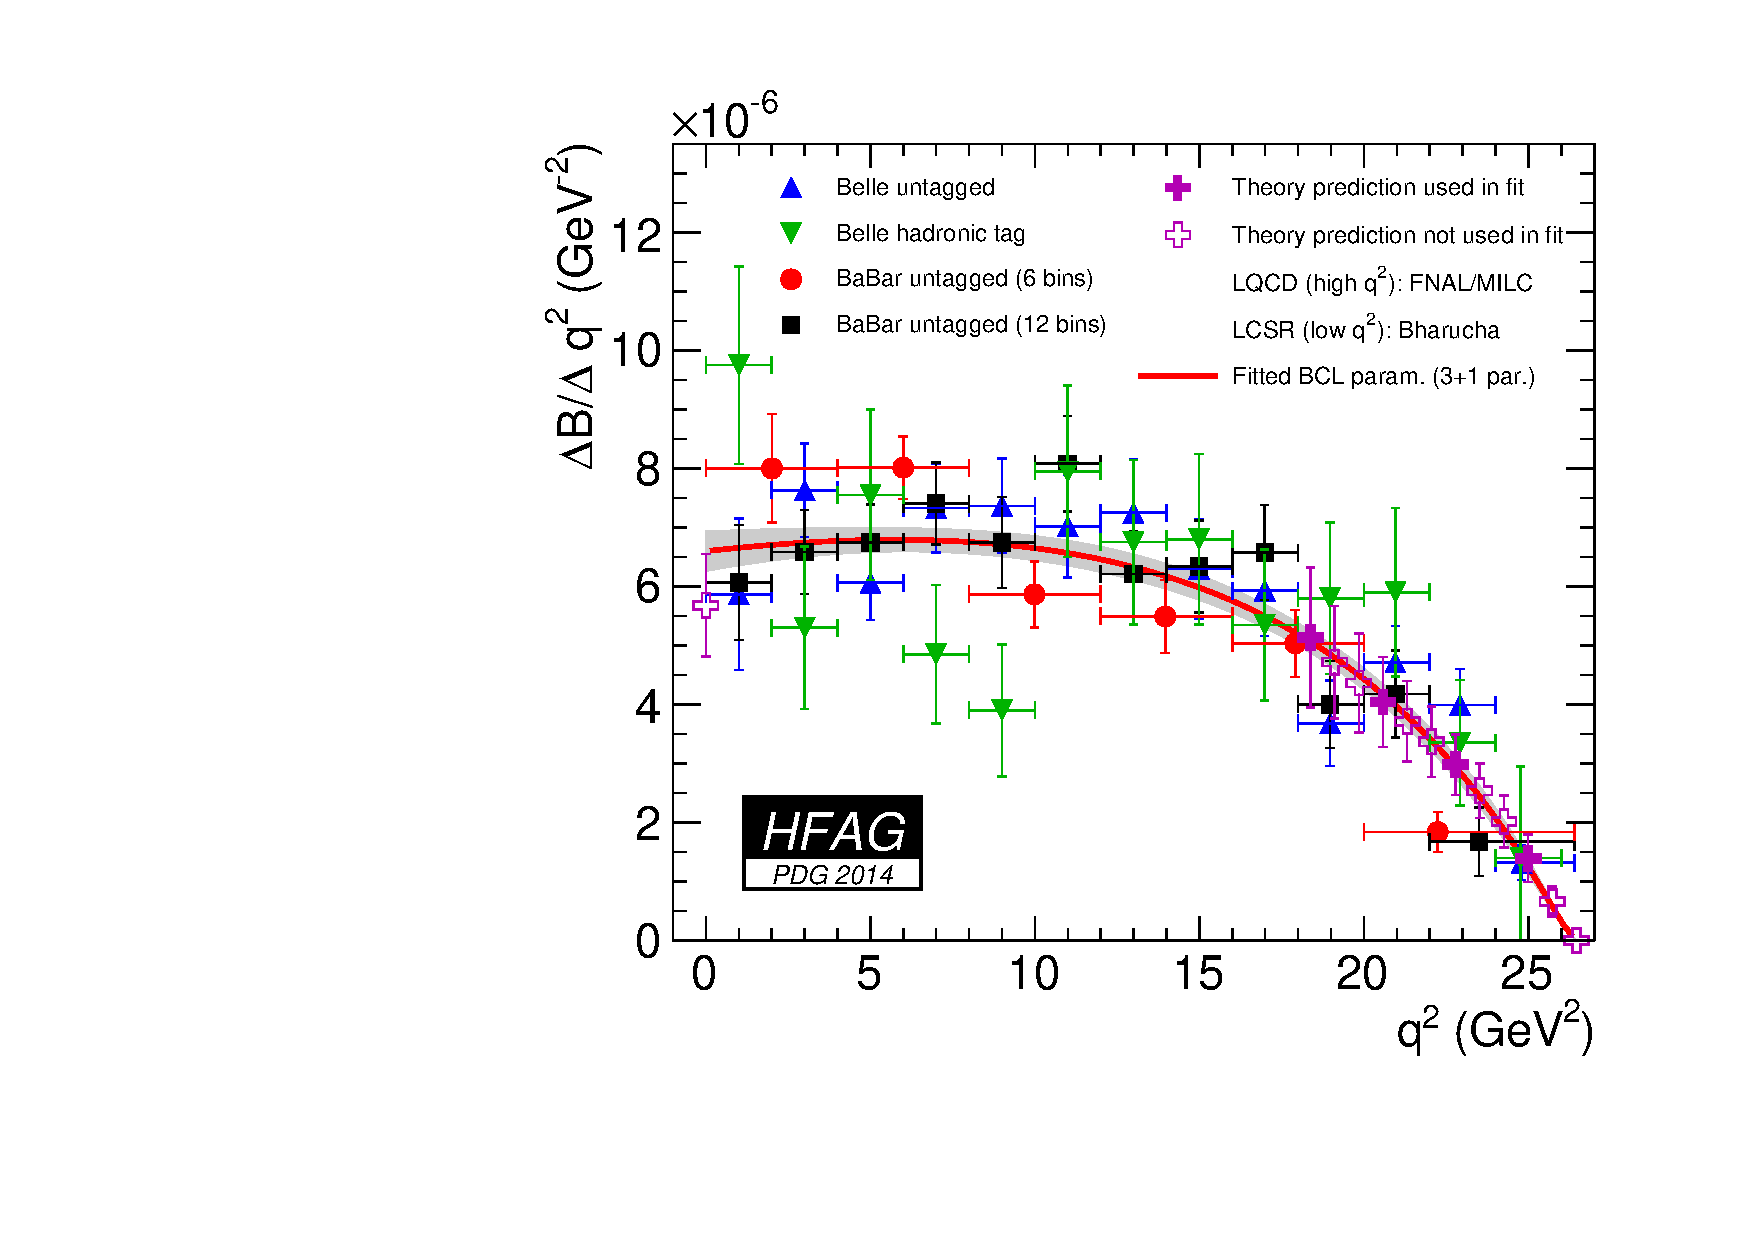
\includegraphics[width=8.0cm]{figures/slb/vub_pilnu_combinedFit_FNAL.pdf}}
   \put( 8.0,  0.0){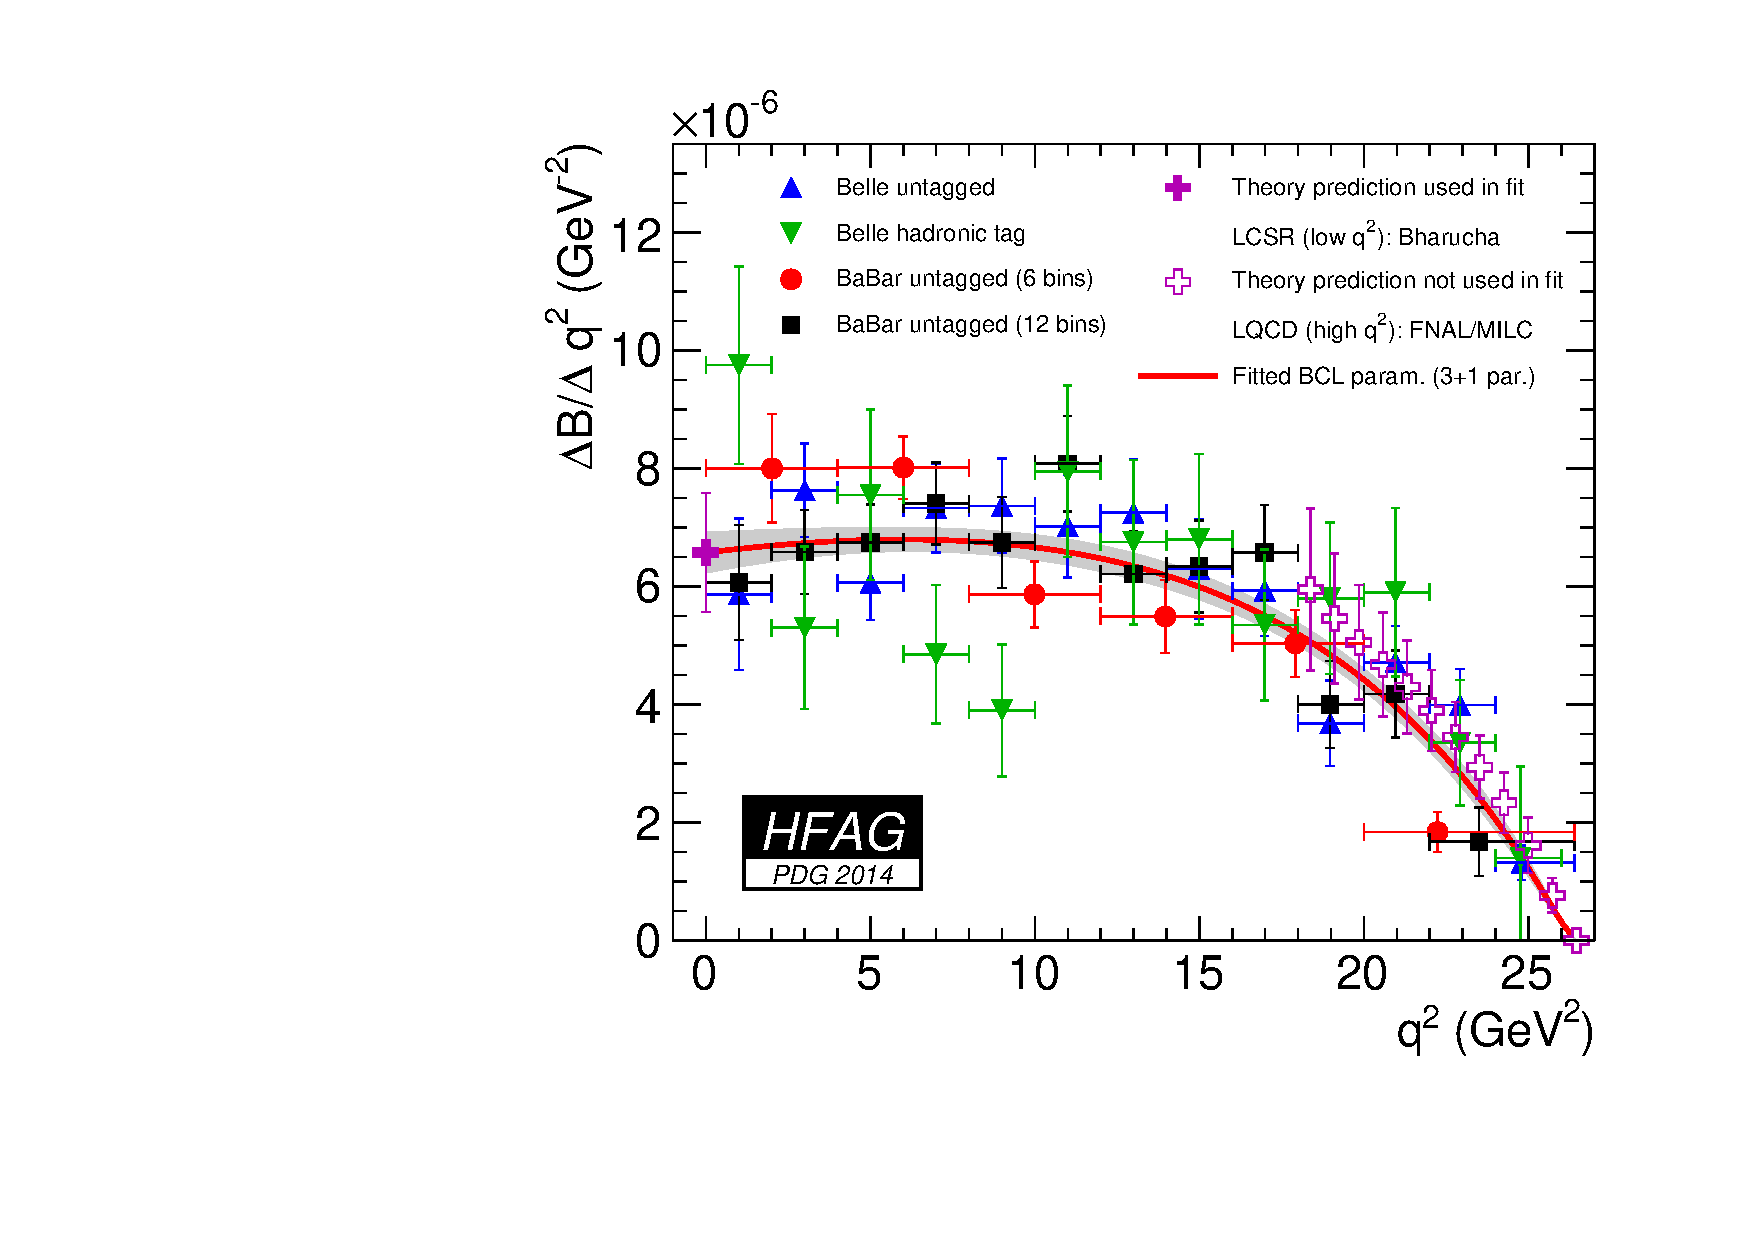
\includegraphics[width=8.0cm]{figures/slb/vub_pilnu_combinedFit_LCSR.pdf}} 
   \put(  5.8,  3.6){{\large\bf a)}}     
   \put( 14.3,  3.6){{\large\bf b)}}
   \end{picture} 
   \caption{
    Simultaneous fit of the BCL parameterization with 3+1 parameters to \babar and Belle $\Bb\to\pi\ell\nub$ data
    and the theory prediction from (a) FNAL/MILC LQCD calculations~\cite{Bailey:2008wp} 
    (yielding $\Vub = (3.28 \pm 0.29) \times 10^{-3}$)
    and (b) LCSR~\cite{Bharucha:2012wy} at $q^2=0$ (yielding $\Vub = (3.53 \pm 0.29) \times 10^{-3}$).}
\label{fig:vub_pilnu_simultaneous}
\end{center}
\end{figure}

The simultaneous fit has also been performed using the most recent result for $f_+(0)$ from LCSR~\cite{Bharucha:2012wy}
($f_+(0) = 0.261^{+0.020}_{-0.023}$), i.e. one point at $q^2=0$ is used as form factor normalization instead of the LQCD points at high $q^2$.
This fit has a probability of 0.029 ($\chi^2/dof = 59.8/41$) and yields consistent results (Fig.~\ref{fig:vub_pilnu_simultaneous}~(b)):
\begin{eqnarray}
\Vub &=& (3.53 \pm 0.29) \times 10^{-3}, \\
b_1/b_0 &=& -0.99 \pm 0.20, \\
b_2/b_0 &=& -1.28 \pm 0.61, \\
f_+(0)\Vub &=& (0.922 \pm 0.024) \times 10^{-3}. 
\end{eqnarray}\\

The branching fractions for 
$\Bb\to \rho\ell\nub$ decays is computed based on the measurements in
Table~\ref{tab:rholnu} and is shown in Figure~\ref{fig:xulnu1}. The determination of $\Vub$
from these other channels looks less promising than for $\Bb\to\pi\ell\nub$ and at the moment it is not extracted.

\input{tables/slb/rholnu.tex}

We also report the branching fraction average for $\Bb\to\omega\ell\nub$, $\Bb\to\eta\ell\nub$ 
and $\Bb\to\eta'\ell\nub$. The measurements for $\Bb\to\omega\ell\nub$ are reported in Table~\ref{tab:omegalnu} 
and shown in Figure~\ref{fig:xulnu1}, while the ones for $\Bb\to\eta\ell\nub$ and  $\Bb\to\eta'\ell\nub$ are reported in Table~\ref{tab:etalnu} and~\ref{tab:etaprimelnu},  and are shown in Figure~\ref{fig:xulnu2}. 

\input{tables/slb/omegalnu.tex}
\input{tables/slb/etalnu.tex}
\input{tables/slb/etaprimelnu.tex}

\begin{figure}[!ht]
 \begin{center}
  \unitlength1.0cm % coordinates in cm
  \begin{picture}(14.,8.0)  %ys(25.,6.)
   \put( -0.5,  0.0){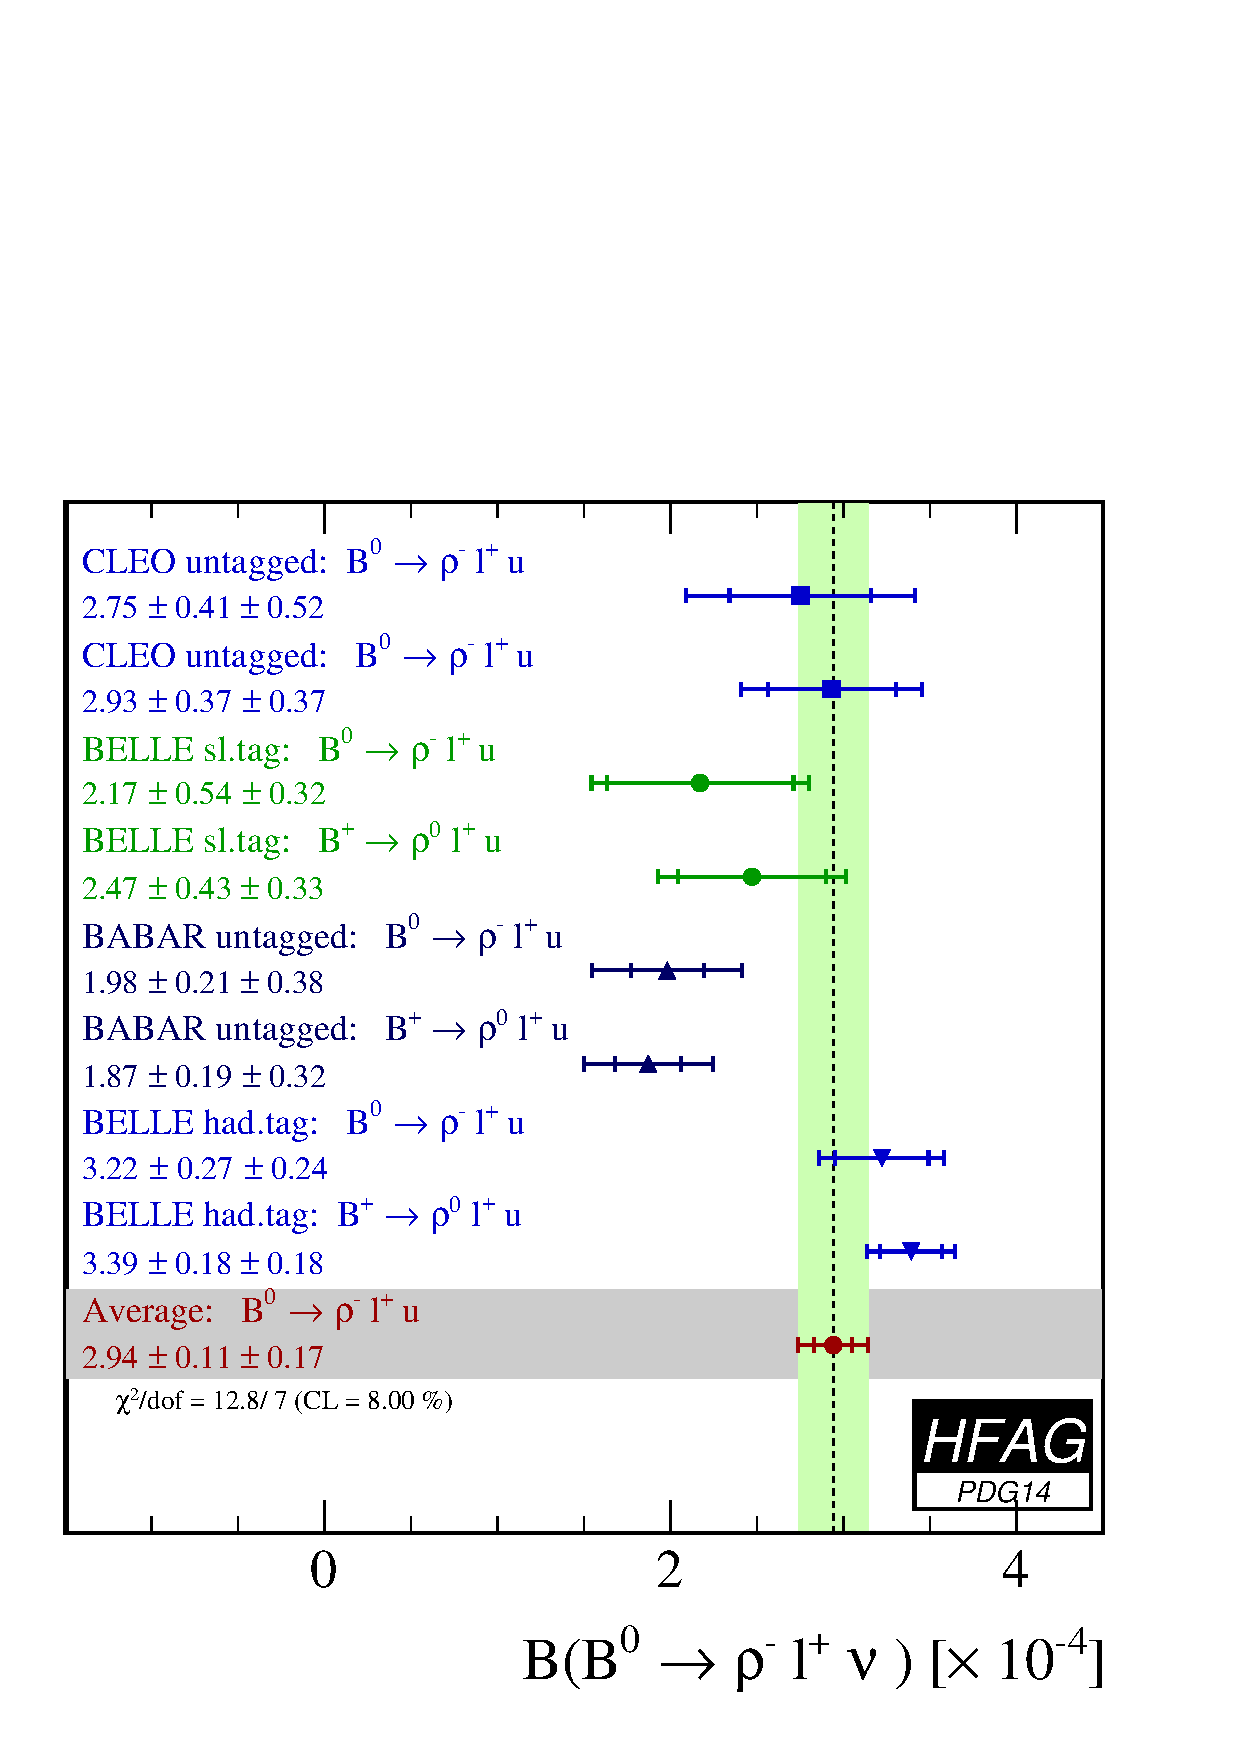
\includegraphics[width=8.0cm]{figures/slb/rholnu.pdf}}
   \put( 8.0,  0.0){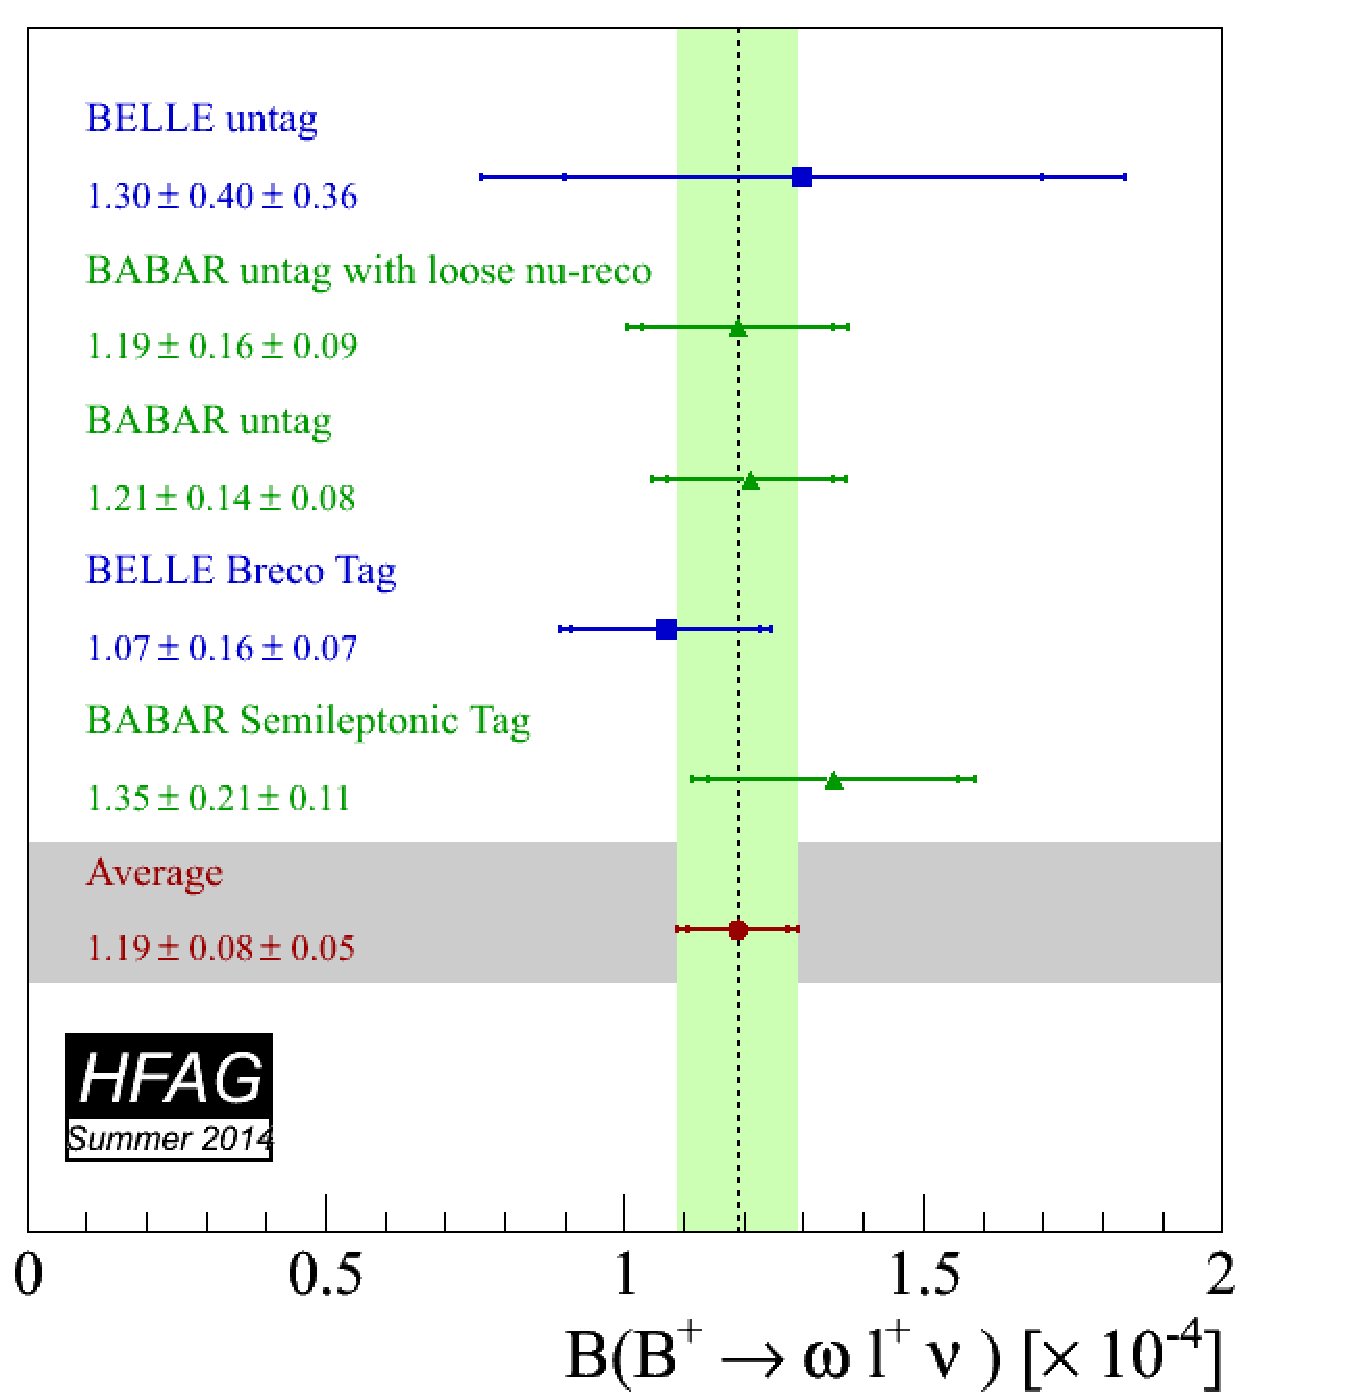
\includegraphics[width=8.0cm]{figures/slb/omegalnu.pdf}} 
   \put(  5.8,  7.5){{\large\bf a)}}  
   \put( 14.4,  7.5){{\large\bf b)}}
   \end{picture} \caption{
 (a) Summary of exclusive determinations of $\cbf(\Bb\to\rho\ell\nub)$ and their average. Measurements
 of $B^+ \to \rho^0\ell^+\nu$ branching fractions have been multiplied by $2\tau_{B^0}/\tau_{B^+}$ 
 in accordance with isospin symmetry.    
(b) Summary of exclusive determinations of $\cbf(\Bb\to\omega\ell\nub)$ and their average.
}
\label{fig:xulnu1}
\end{center}
\end{figure}

\begin{figure}[!ht]
 \begin{center}
  \unitlength1.0cm % coordinates in cm
  \begin{picture}(14.,8.0)  %ys(25.,6.)
   \put( -0.5,  0.0){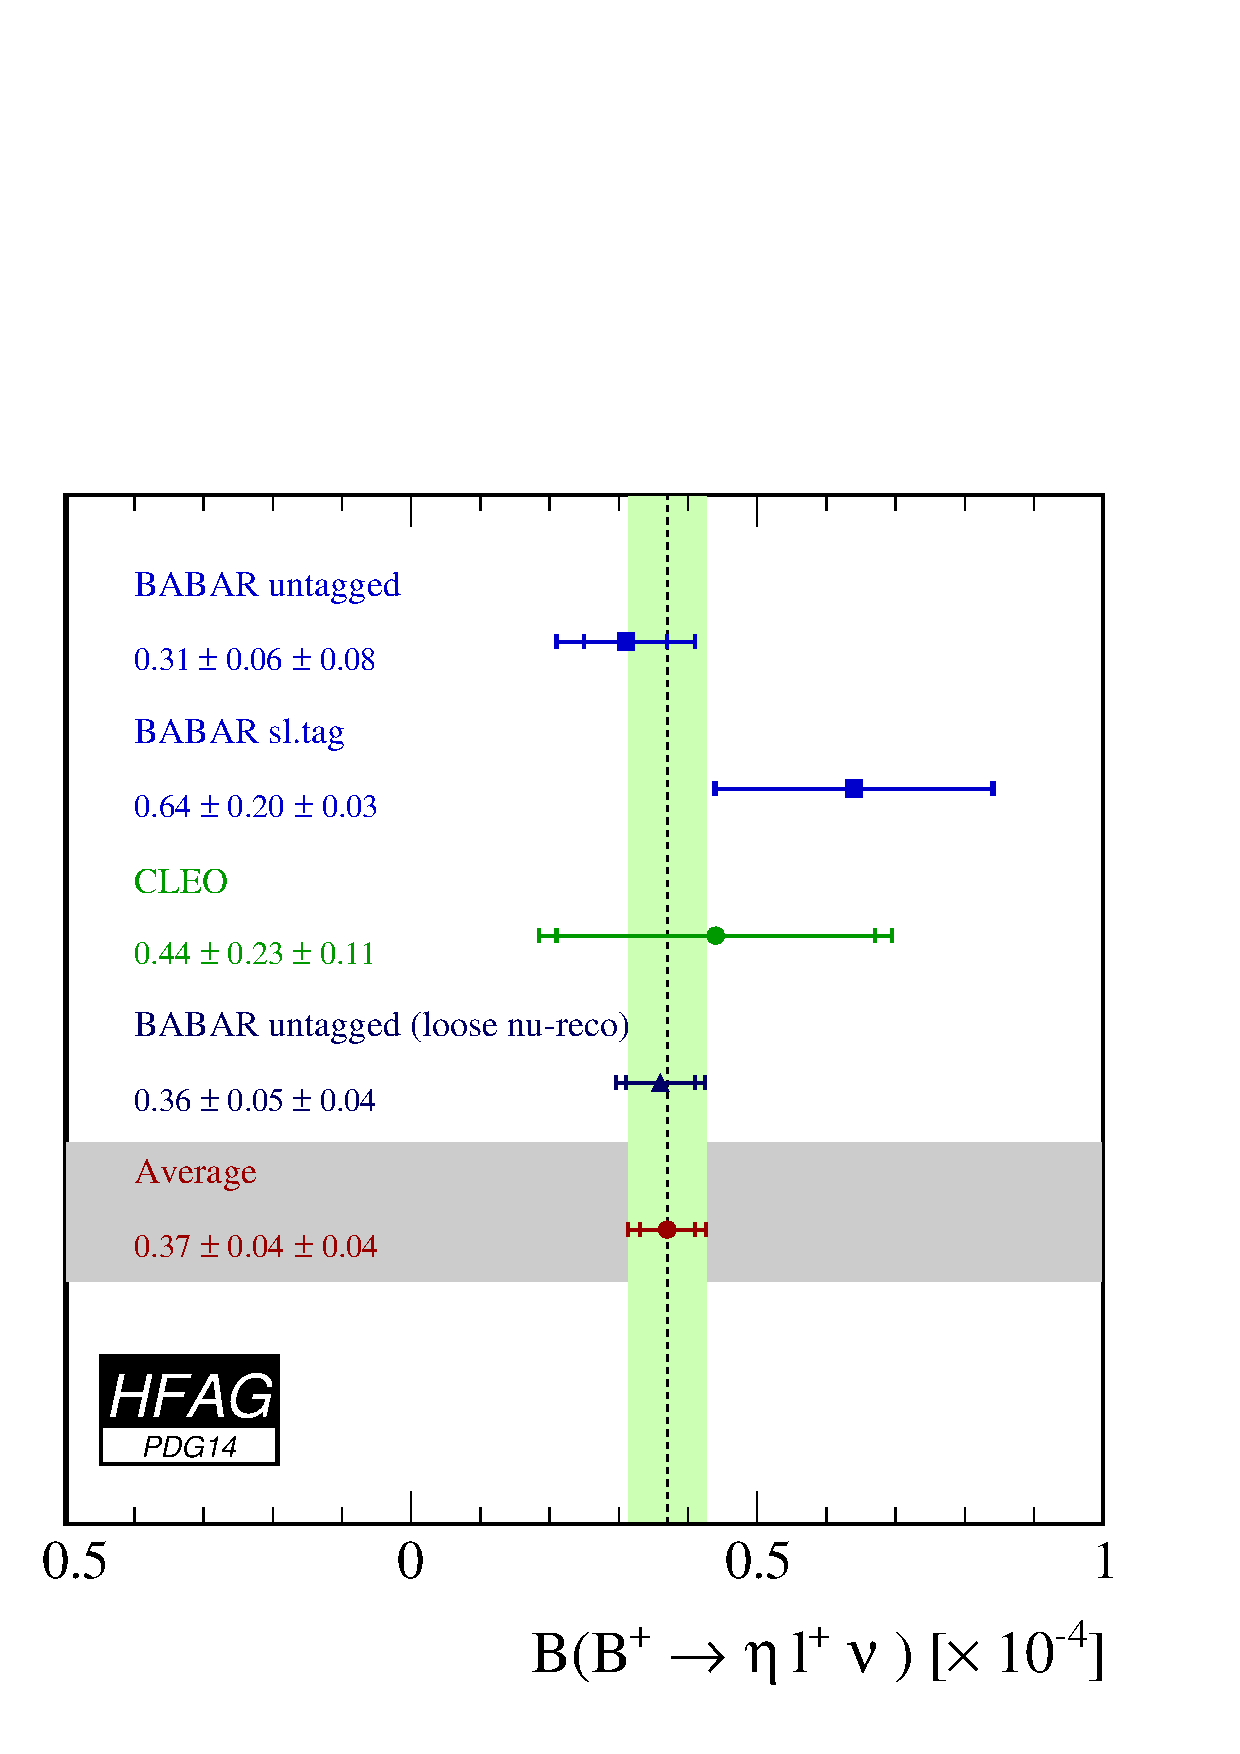
\includegraphics[width=8.0cm]{figures/slb/etalnu.pdf}}
   \put( 8.0,  0.0){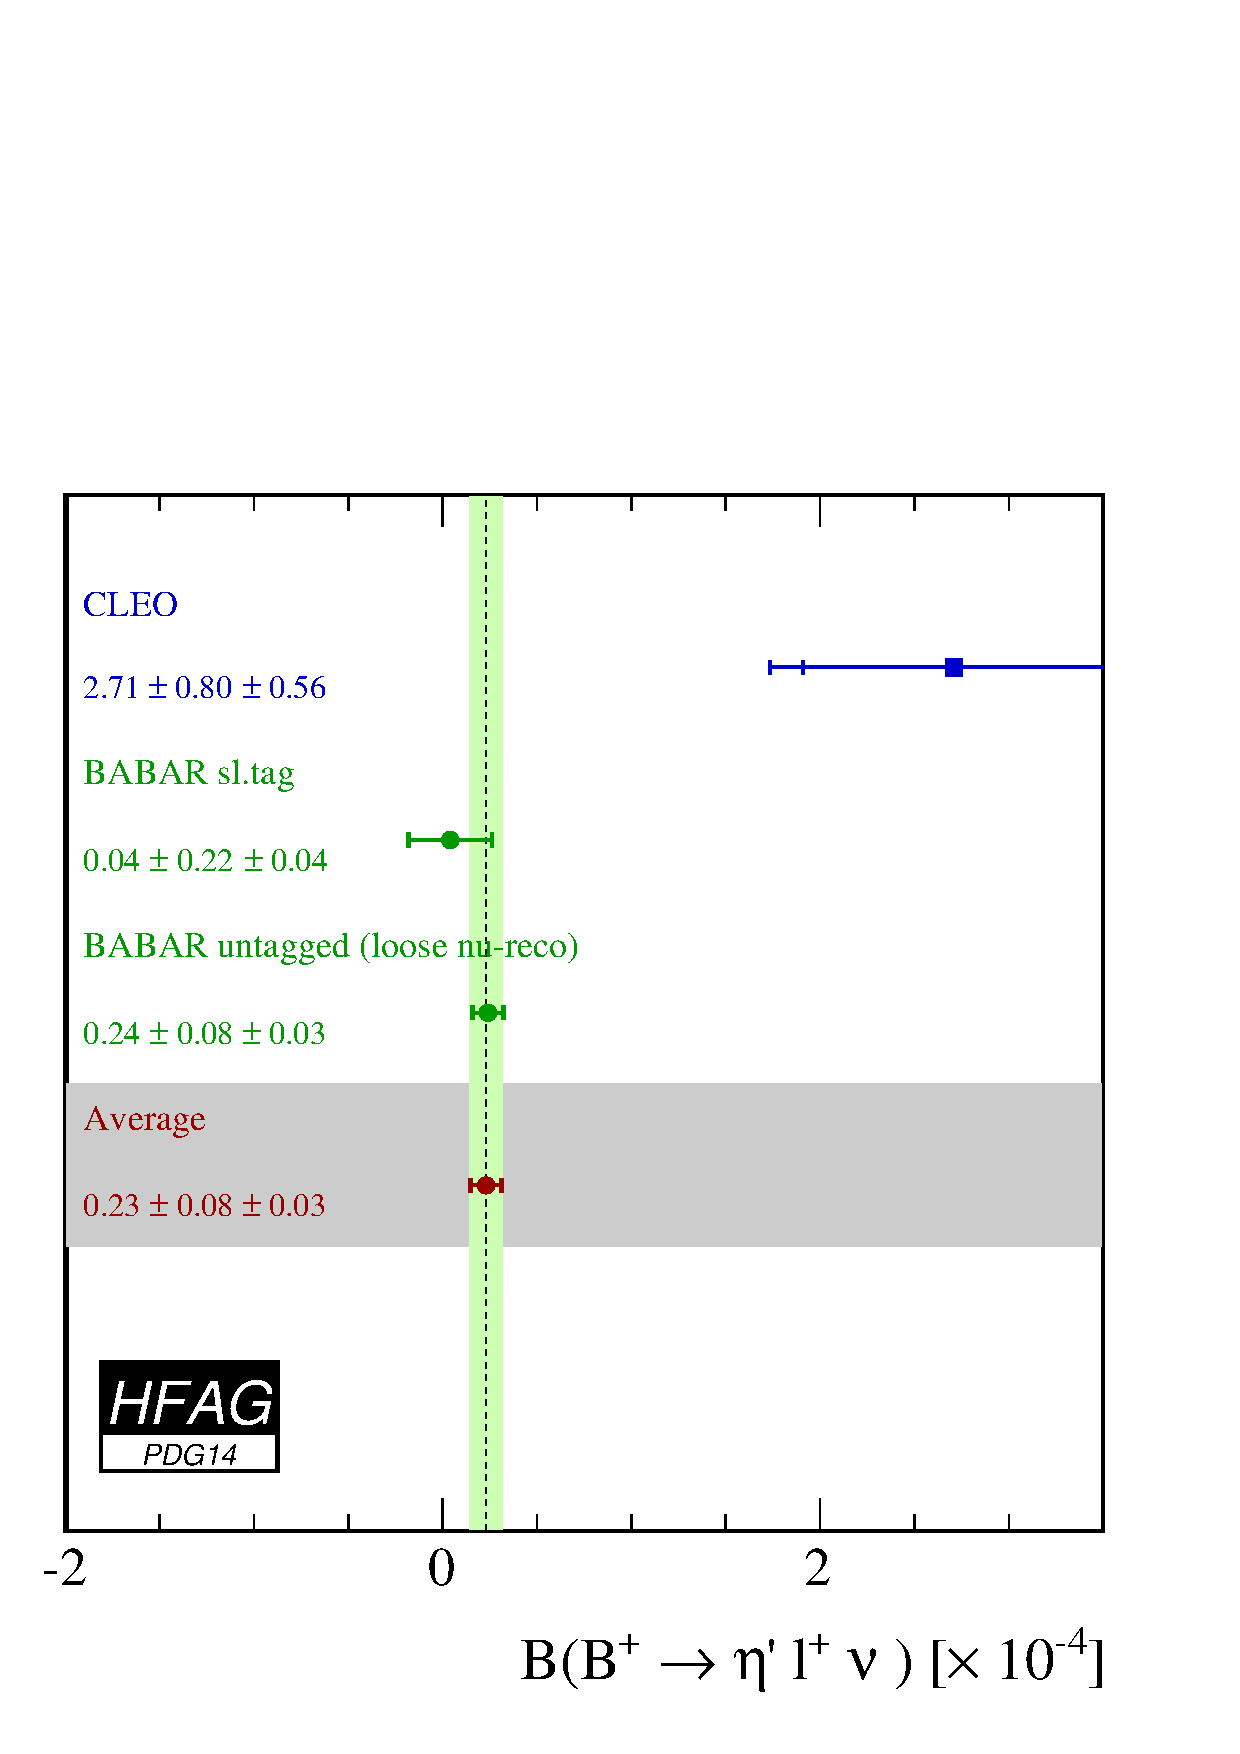
\includegraphics[width=8.0cm]{figures/slb/etaprimelnu.pdf}} 
   \put(  5.5,  7.3){{\large\bf a)}}     
   \put( 14.4,  7.3){{\large\bf b)}}
   
   \end{picture} \caption{
(a) Summary of exclusive determinations of $\cbf(\Bb\to\eta\ell\nub)$ and their average.
(b) Summary of exclusive determinations of $\cbf(\Bb\to\eta'\ell\nub)$ and their average.
}
\label{fig:xulnu2}
\end{center}
\end{figure}

%Branching fractions for other $\Bb\to X_u\ell\nub$ decays are given in
%Table~\ref{tab:xslother}. 
%\input{tables/slb/xslother.tex}

% ----------------------------------------------------------------------


%
% ======================================================================
% Inclusive CKM-suppressed decays
% -- \include{b2uincl.tex}
% ======================================================================
\subsection{Inclusive CKM-suppressed decays}
\label{slbdecays_b2uincl}
% ----------------------------------------------
The large background from $\B\to X_c\ell^+\nul$ decays is the chief
experimental limitation in determinations of $\vub$.  Cuts designed to
reject this background limit the acceptance for $\B\to X_u\ell^+\nul$
decays. The calculation of partial rates for these restricted
acceptances is more complicated and requires substantial theoretical machinery.
In this update, we use several theoretical calculations
to extract \vub. We do not advocate the use of one method over another.
The authors for the different calculations have provided 
codes to compute the partial rates in limited regions of phase space covered by the measurements. 
Latest results by Belle~\cite{ref:belle-multivariate} and \babar~\cite{ref:babar-finalupdate} 
explore bigger and bigger portions of phase space, with a consequent reduction of the theoretical 
uncertainties. 

For the averages we performed, the systematic errors associated with the
modeling of $\B\to X_c\ell^+\nul$ and $\B\to X_u\ell^+\nul$ decays and the theoretical
uncertainties are taken as fully correlated among all measurements.
Reconstruction-related uncertainties are taken as fully correlated within a given experiment.
We use all results published by \babar\ in~\cite{ref:babar-finalupdate}, since the 
statistical correlations are given. 
To make use of the theoretical calculations of Ref.~\cite{ref:BLL}, we restrict the
kinematic range in $M_X$ and $q^2$, thereby reducing the size of the data
sample significantly, but also the theoretical uncertainty, as stated by the
authors~\cite{ref:BLL}.
The dependence of the quoted error on the measured value for each source of error
is taken into account in the calculation of the averages.
Measurements of partial branching fractions for $\B\to X_u\ell^+\nul$
transitions from $\Upsilon(4S)$ decays, together with the corresponding accepted region, 
are given in Table~\ref{tab:BFbulnu}.  
The signal yields for all the measurements shown in Table~\ref{tab:BFbulnu}
are not rescaled to common input values of the $B$ meson lifetime (see Sect.~\ref{sec:life_mix})
%  replace with PDG_2008 which is in EndOfYear2011.bib 
% and the semileptonic width~\cite{PDG_2007}.
and the semileptonic width~\cite{PDG_2008}.

It has been first suggested by Neubert~\cite{Neubert:1993um} and later detailed by Leibovich, 
Low, and Rothstein (LLR)~\cite{Leibovich:1999xf} and Lange, Neubert and Paz (LNP)~\cite{Lange:2005qn}, 
that the uncertainty of
the leading shape functions can be eliminated by comparing inclusive rates for
$\B\to X_u\ell^+\nul$ decays with the inclusive photon spectrum in $\B\to X_s\gamma$,
based on the assumption that the shape functions for transitions to light
quarks, $u$ or $s$, are the same to first order.
However, shape function uncertainties are only eliminated at the leading order
and they still enter via the signal models used for the determination of efficiency. 
For completeness, we provide a comparison of the results using 
calculations with reduced dependence on the shape function, as just
introduced, with our averages using different theoretical approaches.
Results are presented by \babar\ in Ref.\cite{Aubert:2006qi} using the LLR prescription. 
In another work (Ref.~\cite{Golubev:2007cs}), \vub\ was extracted from the 
endpoint spectrum of $\B\to X_u\ell^+\nul$ from \babar~\cite{ref:babar-endpoint}, 
using several theoretical approaches with reduced dependence on the shape function.
In both cases, the photon energy spectrum in the 
rest frame of the $B$-meson by \babar~\cite{Aubert:2005cua} has been used.


\input{tables/slb/bulnu.tex}


\subsubsection{BLNP}
Bosch, Lange, Neubert and Paz (BLNP)~\cite{ref:BLNP,
% removed missing reference TJG 13/5/2012
%  ref:Neubert-new-1,ref:Neubert-new-2,ref:Neubert-new-3,ref:Neubert-new-4}
  ref:Neubert-new-1,ref:Neubert-new-2,ref:Neubert-new-3}
provide theoretical expressions for the triple
differential decay rate for $B\to X_u \ell^+ \nul$ events, incorporating all known
contributions, whilst smoothly interpolating between the 
``shape-function region'' of large hadronic
energy and small invariant mass, and the ``OPE region'' in which all
hadronic kinematical variables scale with the $b$-quark mass. BLNP assign
uncertainties to the $b$-quark mass which enters through the leading shape function, 
to sub-leading shape function forms, to possible weak annihilation
contribution, and to matching scales. 
The BLNP calculation uses the shape function renormalization scheme; the heavy quark parameters determined  
from the global fit in the kinetic scheme, described in \ref{globalfitsKinetic}, were therefore 
translated into the shape function scheme by using a prescription by Neubert 
\cite{Neubert:2004sp,Neubert:2005nt}. The resulting parameters are 
$m_b(SF)=(4.569 \pm 0.023 \pm 0.018)$ GeV, 
$\mu_\pi^2(SF)=(0.145 \pm 0.089 ^{+0.020}_{-0.040})$ GeV$^2$, 
where the second uncertainty is due to the scheme translation. 
The extracted values of \vub\, for each measurement along with their average are given in
Table~\ref{tab:bulnu} and illustrated in Figure~\ref{fig:BLNP_DGE}(a). 
The total uncertainty is $^{+5.8}_{-5.9}\%$ and is due to:
statistics ($^{+2.0}_{-2.1}\%$),
detector ($^{+1.7}_{-1.8}\%$),
$B\to X_c \ell^+ \nul$ model ($^{+1.2}_{-1.2}\%$),
$B\to X_u \ell^+ \nul$ model ($^{+1.9}_{-1.8}\%$),
heavy quark parameters ($^{+2.6}_{-2.7}\%$),
SF functional form ($^{+0.1}_{-0.3}\%$),
sub-leading shape functions ($^{+0.6}_{-0.6}\%$),
BLNP theory: matching scales $\mu,\mu_i,\mu_h$ ($^{+3.8}_{-3.8}\%$), and
weak annihilation ($^{+0.0}_{-1.4}\%$).
The error on the HQE parameters ($b$-quark mass and $\mu_\pi^2)$ 
is the source of the largest uncertainty, while the
uncertainty assigned for the matching scales is a close second. The uncertainty due to 
weak annihilation has been assumed to be asymmetric, i.e. it only tends to decrease \vub.

\input{tables/slb/VubIncl.tex}

%\begin{figure}
%\begin{center}
%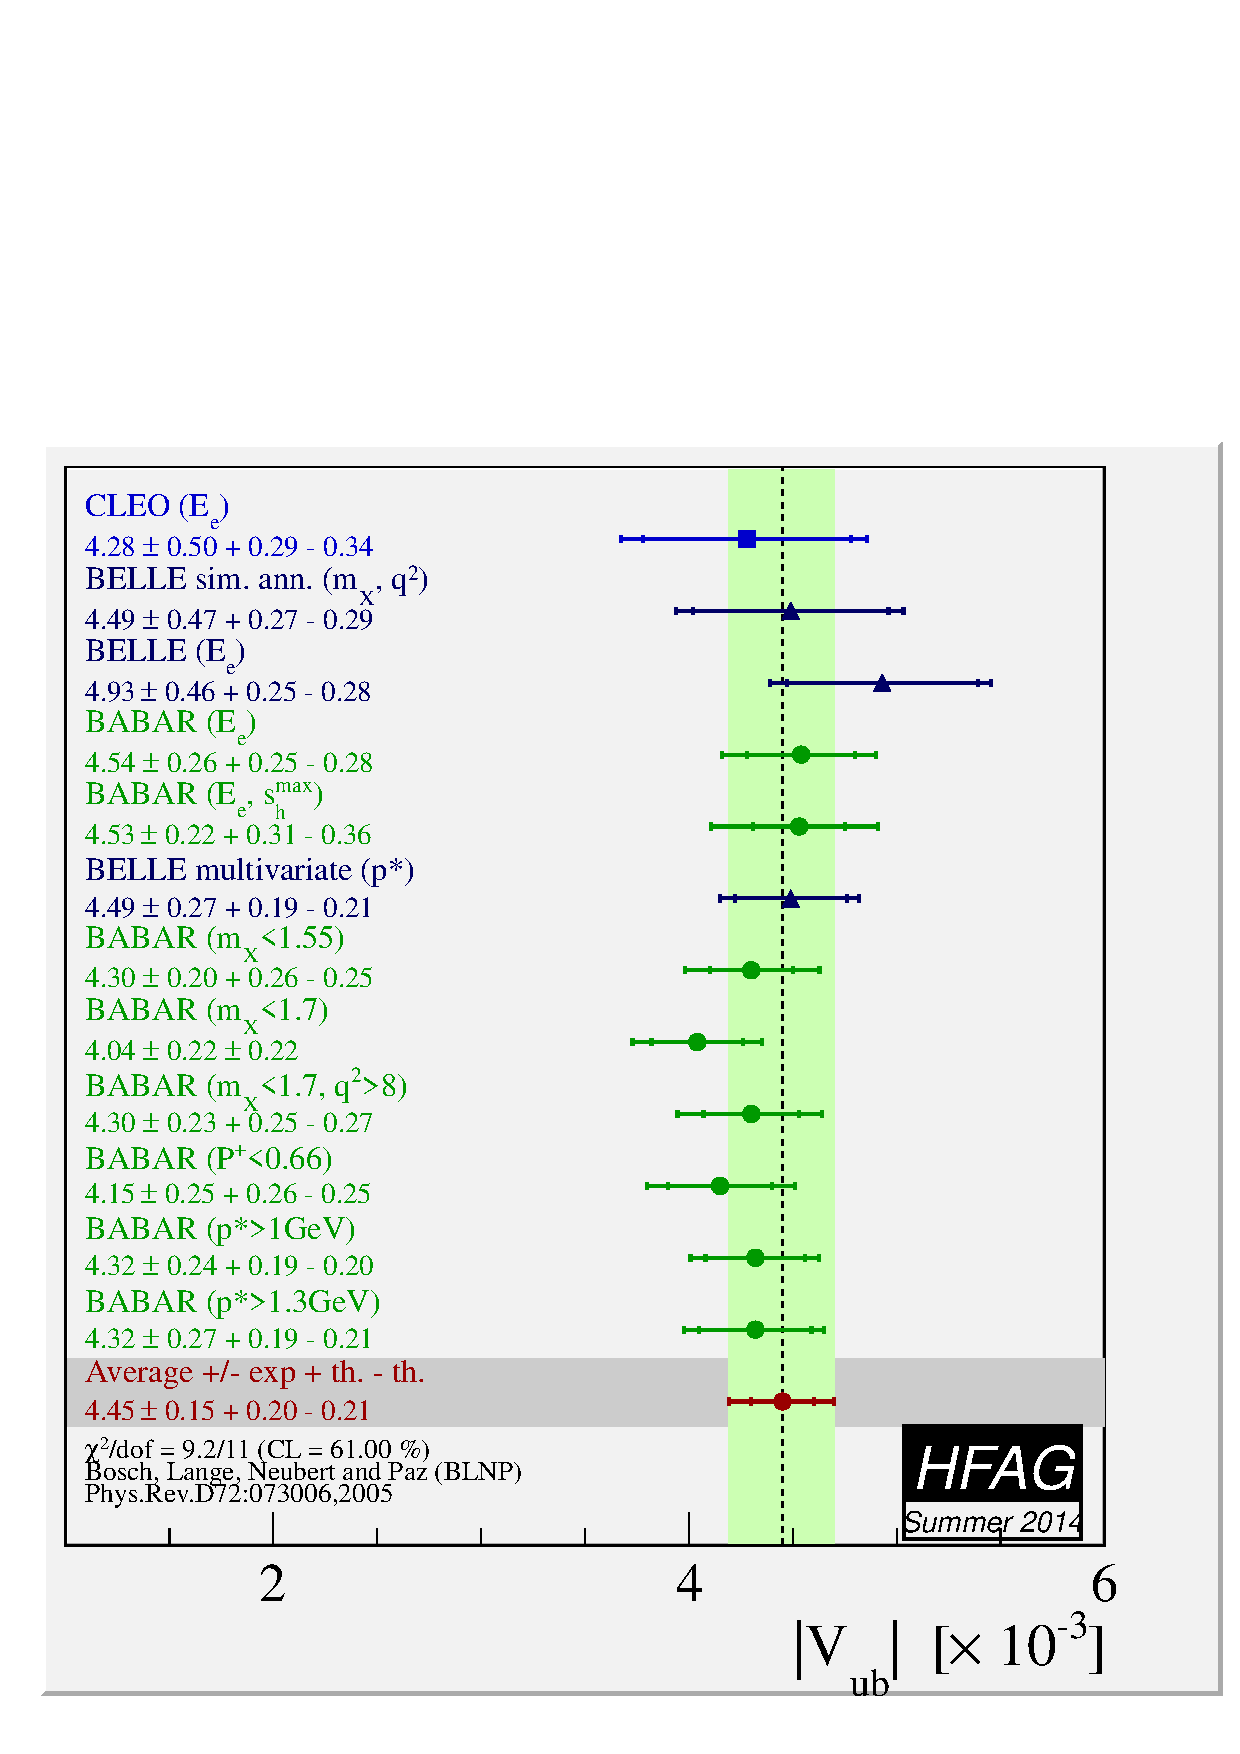
\includegraphics[width=0.48\textwidth]{figures/slb/vub_clnu_mc_twomu_asym_BLNP.pdf}
%\end{center}
%\caption{Measurements of $\vub$ from inclusive semileptonic decays 
%and their average based on the BLNP prescription.
%``$E_e$'', ``$M_X$'', ``$(M_X,q^2)$'', ``$P^+$'', ``$p^*$ and ``($E_e,s^{max}_h$)'' indicate the 
%distributions and cuts used for the measurement of the partial decay rates.}
%\label{fig:BLNP}
%\end{figure}

\begin{figure}[!ht]
 \begin{center}
  \unitlength1.0cm % coordinates in cm
  \begin{picture}(14.,8.0)  %ys(25.,6.0)
   \put( -0.5,  0.0){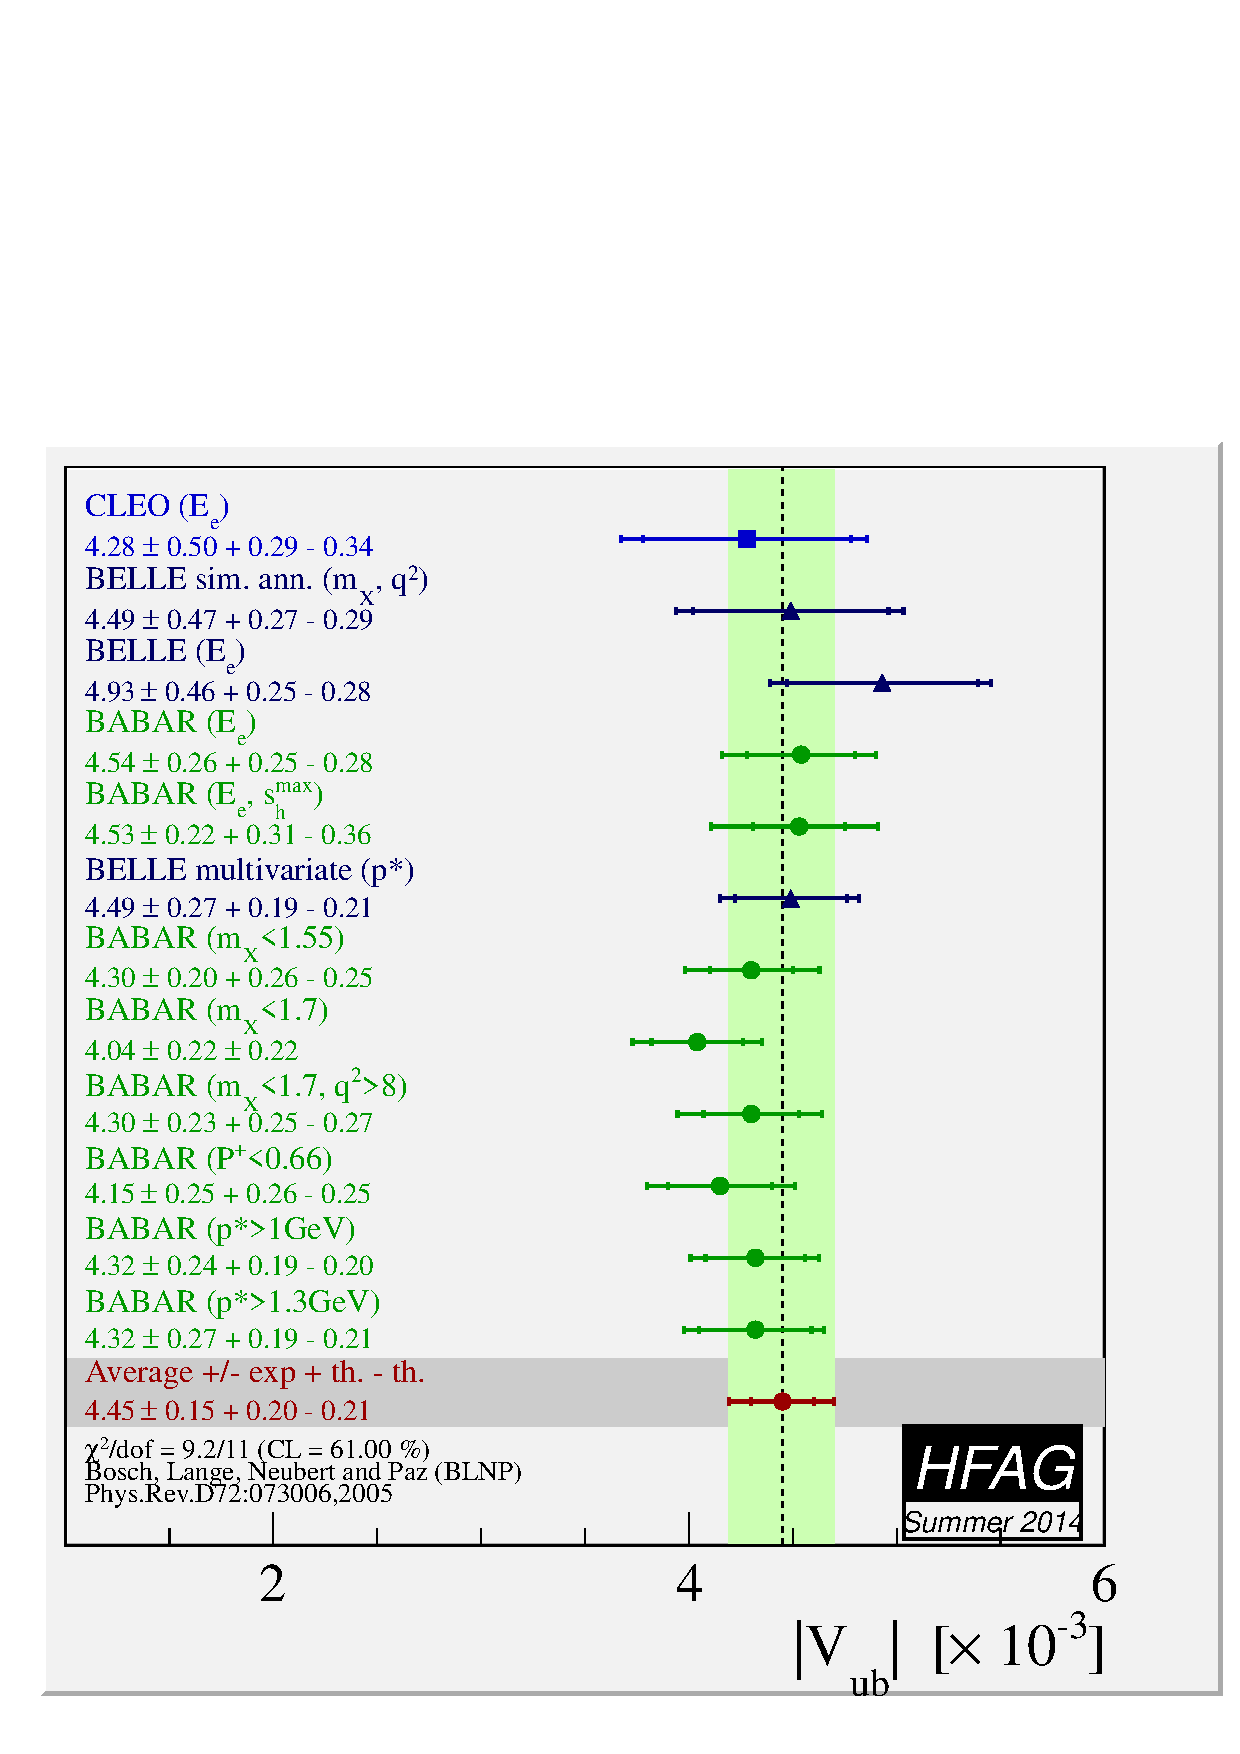
\includegraphics[width=0.48\textwidth]{figures/slb/vub_clnu_mc_twomu_asym_BLNP.pdf}
   }
   \put(  8.0,  0.0){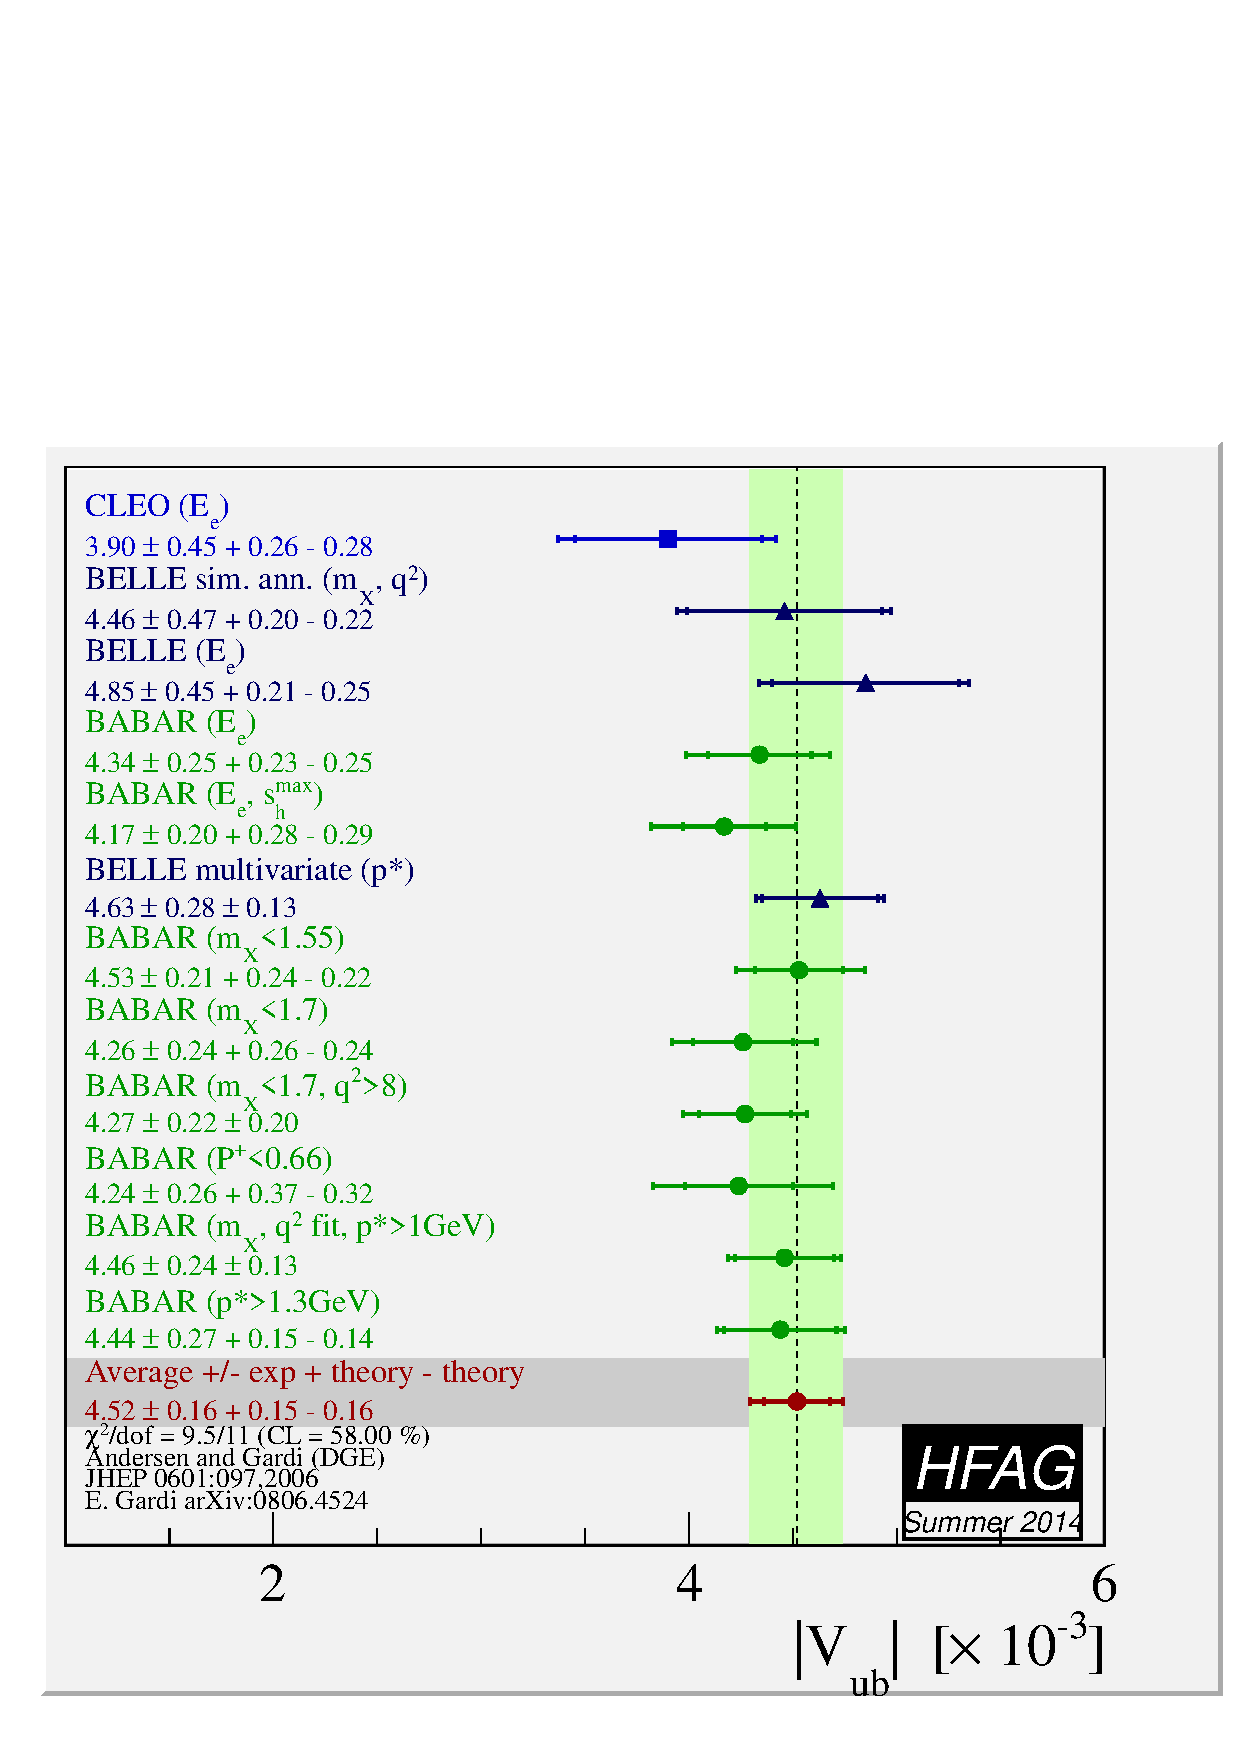
\includegraphics[width=0.47\textwidth]{figures/slb/vub_clnu_mc_asym_DGE.pdf}
   }
   \put(  5.7,  7.8){{\large\bf a)}}
   \put( 14.2,  7.8){{\large\bf b)}}
  \end{picture}
  \caption{Measurements of $\vub$ from inclusive semileptonic decays 
and their average based on the BLNP (a) and DGE (b) prescription.
``$E_e$'', ``$M_X$'', ``$(M_X,q^2)$'', ``$P^+$'', ``$p^*$ and ``($E_e,s^{max}_h$)'' indicate the 
distributions and cuts used for the measurement of the partial decay rates.}
  \label{fig:BLNP_DGE}
 \end{center}
\end{figure}


\begin{figure}[!ht]
 \begin{center}
  \unitlength1.0cm % coordinates in cm
  \begin{picture}(14.,8.0)  %ys(25.,6.0)
   \put( -0.5,  0.0){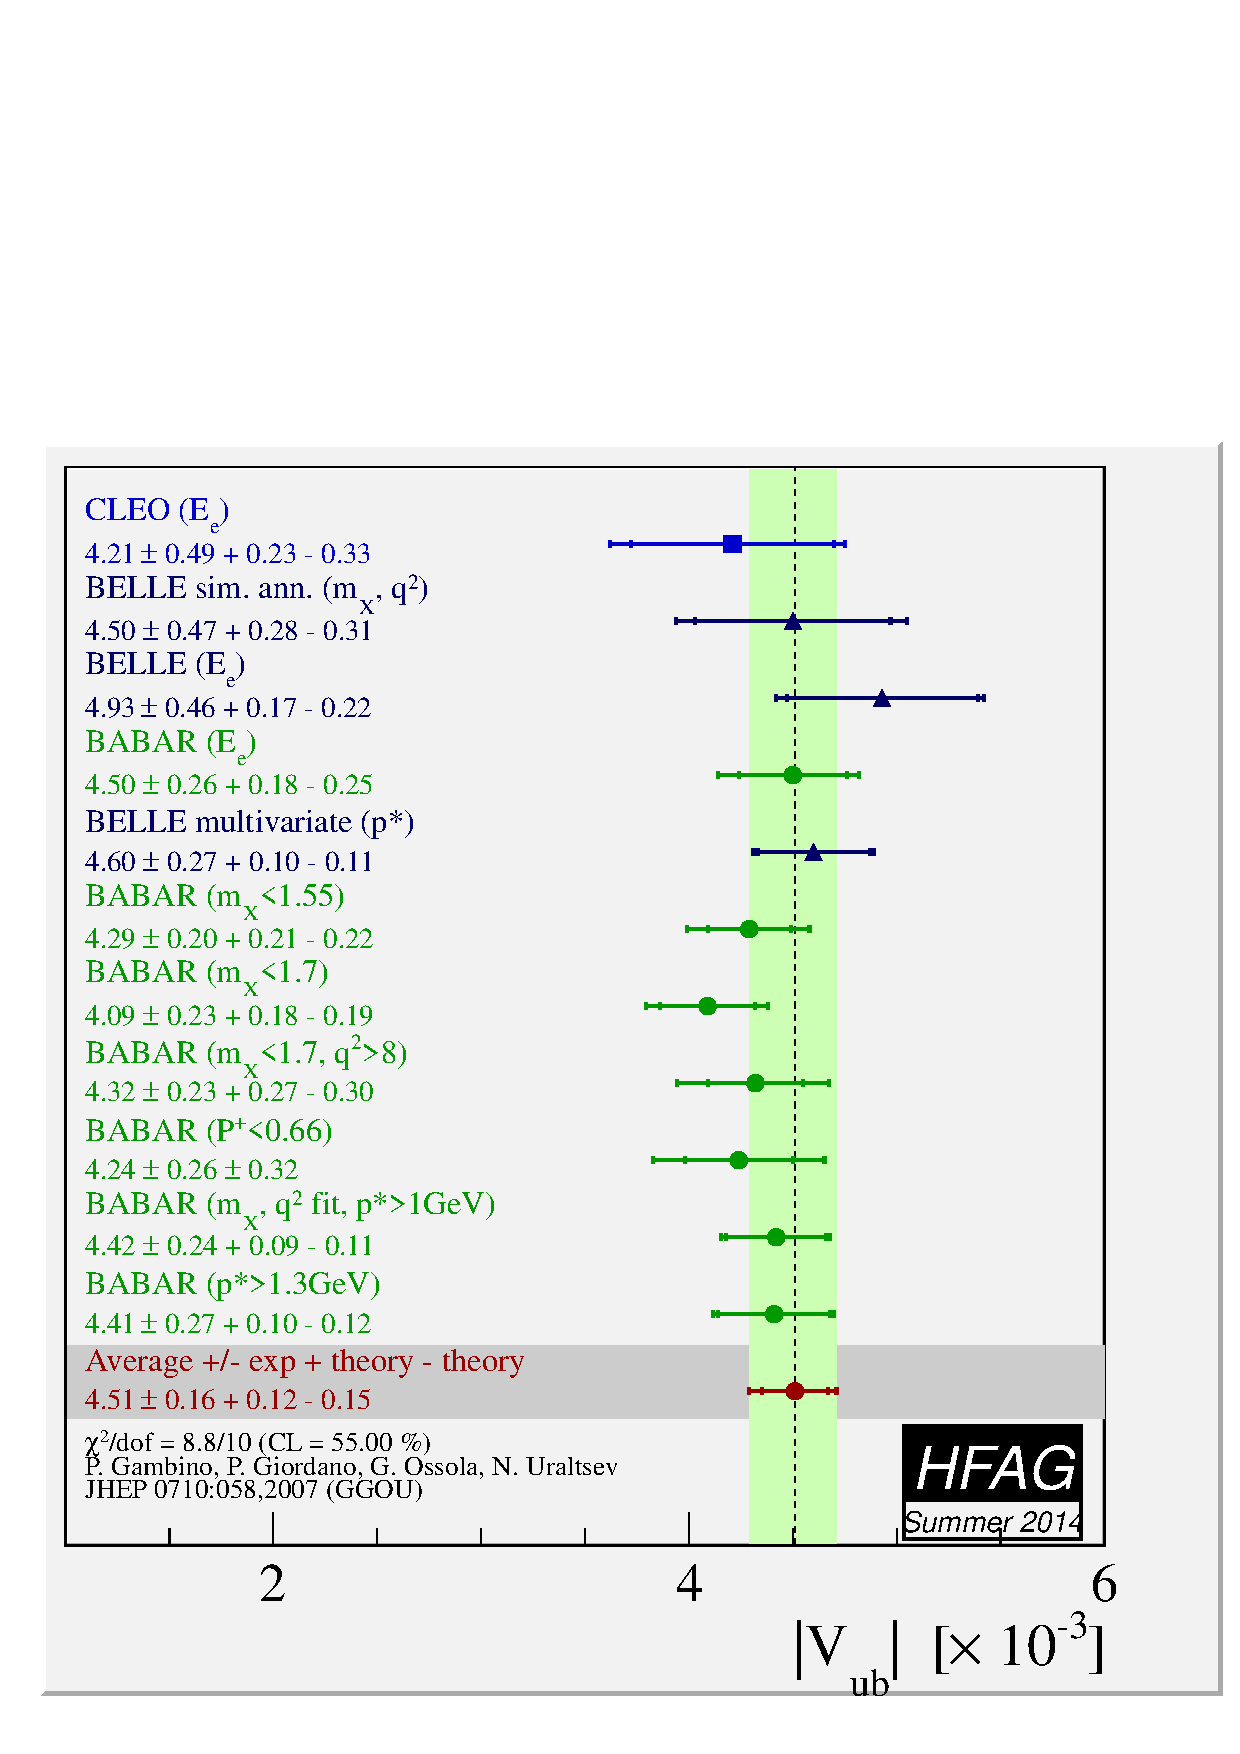
\includegraphics[width=0.48\textwidth]{figures/slb/vub_clnu_mc_GGOU.pdf}
   }
   \put(  8.0,  0.0){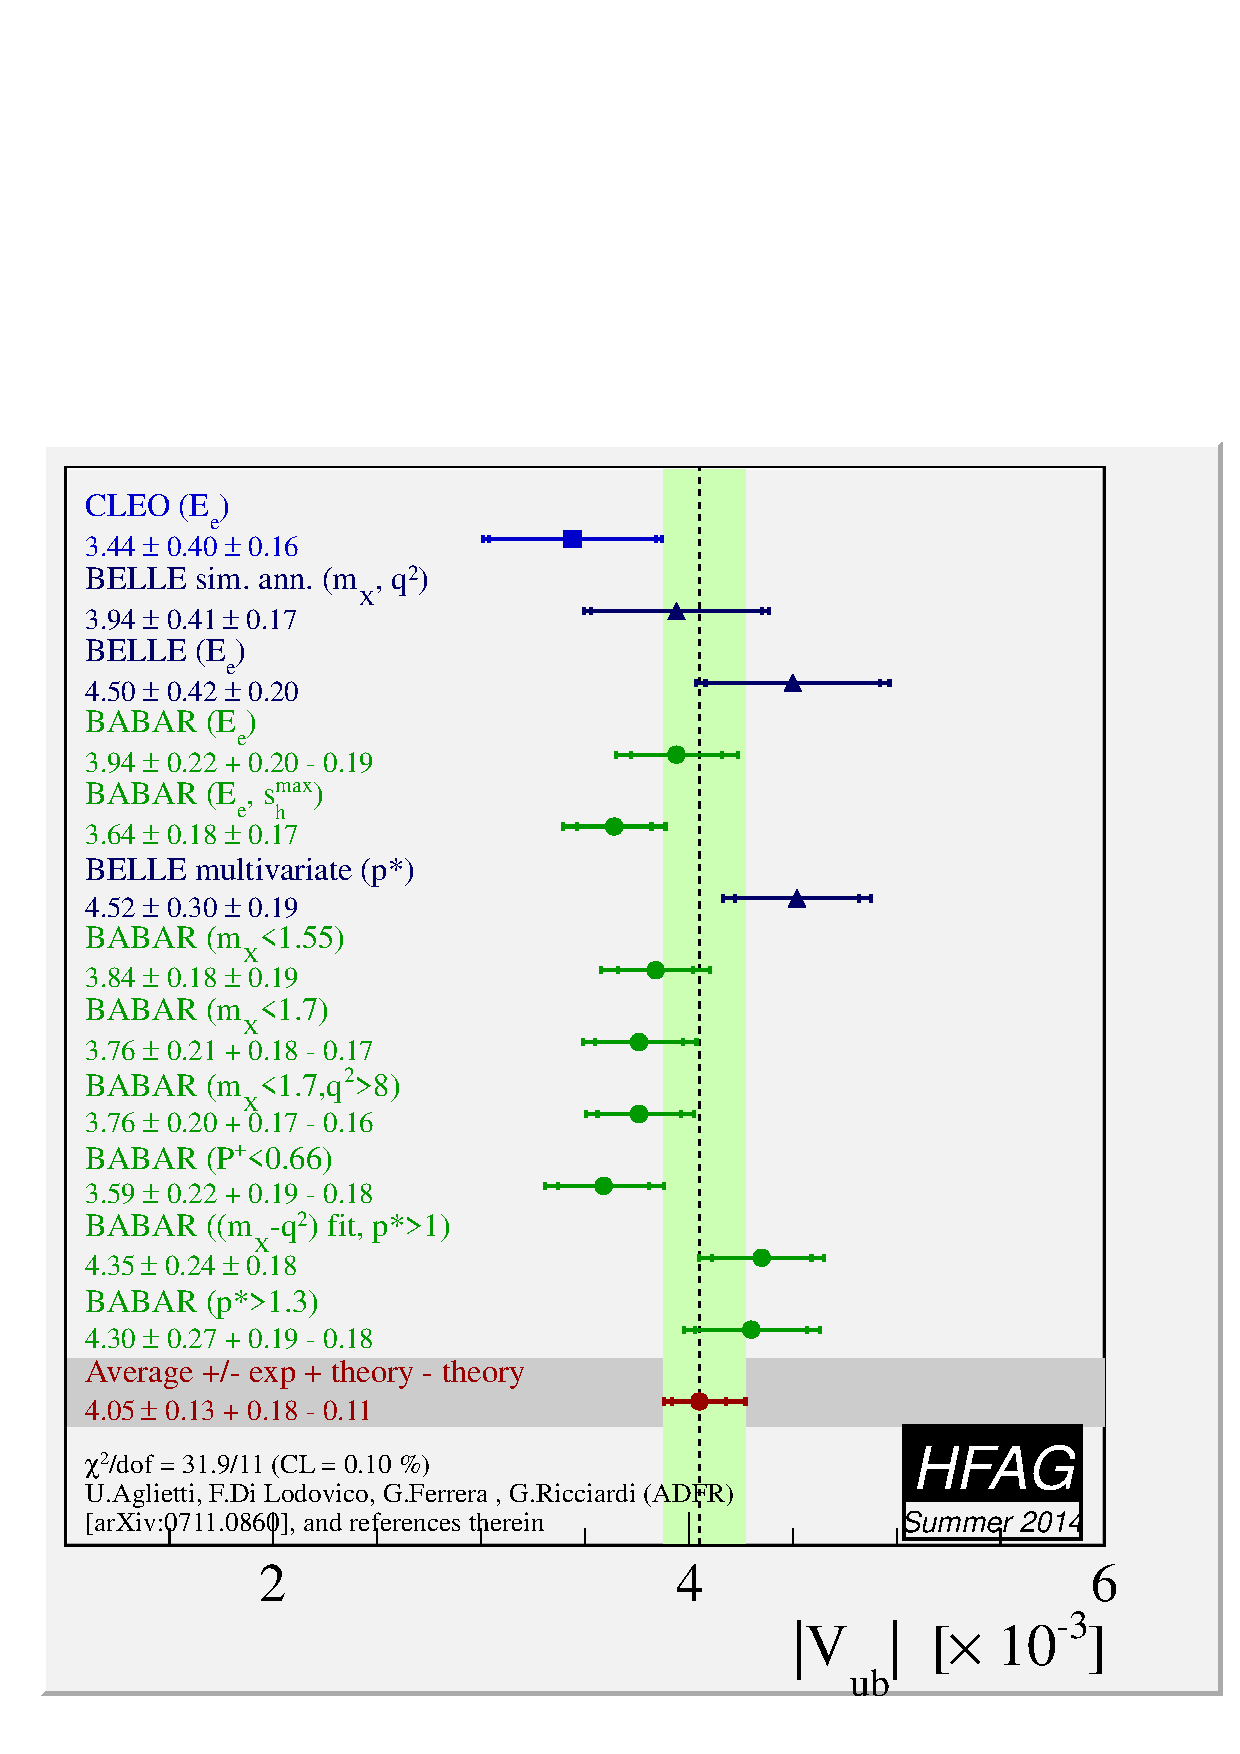
\includegraphics[width=0.48\textwidth]{figures/slb/vub_clnu_mc_ADFR.pdf}
   }
   \put(  5.7,  7.8){{\large\bf a)}}
   \put( 14.2,  7.8){{\large\bf b)}}
  \end{picture}
  \caption{Measurements of $\vub$ from inclusive semileptonic decays 
and their average based on the GGOU (a) and ADFR (b) prescription.
``$E_e$'', ``$M_X$'', ``$(M_X,q^2)$'', ``$P^+$'', ``$p^*$ and ``($E_e,s^{max}_h$)'' indicate the 
distributions and cuts used for the measurement of the partial decay rates.}
  \label{fig:GGOU_ADFR}
 \end{center}
\end{figure}



\subsubsection{DGE}
J.R.~Andersen and E.~Gardi (Dressed Gluon Exponentiation, DGE)~\cite{ref:DGE} provide
a framework where the on-shell $b$-quark calculation, converted into hadronic variables, is
directly used as an approximation to the meson decay spectrum without
the use of a leading-power non-perturbative function (or, in other words,
a shape function). The on-shell mass of the $b$-quark within the $B$-meson ($m_b$) is
required as input. 
The DGE calculation uses the $\overline{MS}$ renormalization scheme; the heavy quark parameters determined  
from the global fit in the kinetic scheme, described in \ref{globalfitsKinetic}, were therefore 
translated into the $\overline{MS}$ scheme by using a calculation by Gardi, giving 
$m_b({\overline{MS}})=(4.177 \pm 0.043)$ GeV.
The extracted values
of \vub\, for each measurement along with their average are given in
Table~\ref{tab:bulnu} and illustrated in Figure~\ref{fig:BLNP_DGE}(b).
The total error is $^{+4.8}_{-5.0}\%$, whose breakdown is:
statistics ($^{+1.8}_{-1.8}\%$),
detector ($^{+1.7}_{-1.7}\%$),
$B\to X_c \ell^+ \nul$ model ($^{+1.3}_{-1.3}\%$),
$B\to X_u \ell^+ \nul$ model ($^{+2.1}_{-1.9}\%$),
strong coupling $\alpha_s$ ($^{+0.5}_{-0.5}\%$),
$m_b$ ($^{+3.2}_{-3.0}\%$),
%%%%%%%%%%%%%%?!?!?!?spectral fraction ($m_b$) ($^{+3.0}_{-3.3}\%$),
%%%%%%%%%%%%%%?!?!?!?!total semileptonic width ($m_b$) ($^{+3.0}_{-3.0}\%$),
weak annihilation ($^{+0.0}_{-1.9}\%$),
DGE theory: matching scales ($^{+0.5}_{-0.3}\%$).
The largest contribution to the total error is due to the effect of the uncertainty 
on $m_b$. 
%%%%%%%%%%%%%%on the prediction of the event rate, closely followed by the 
%%%%%%%%%%%%%%specific theory error on overall DGE and the total semileptonic decay width.
The uncertainty due to 
weak annihilation has been assumed to be asymmetric, i.e. it only tends to decrease \vub.

%\begin{figure}
%\begin{center}
%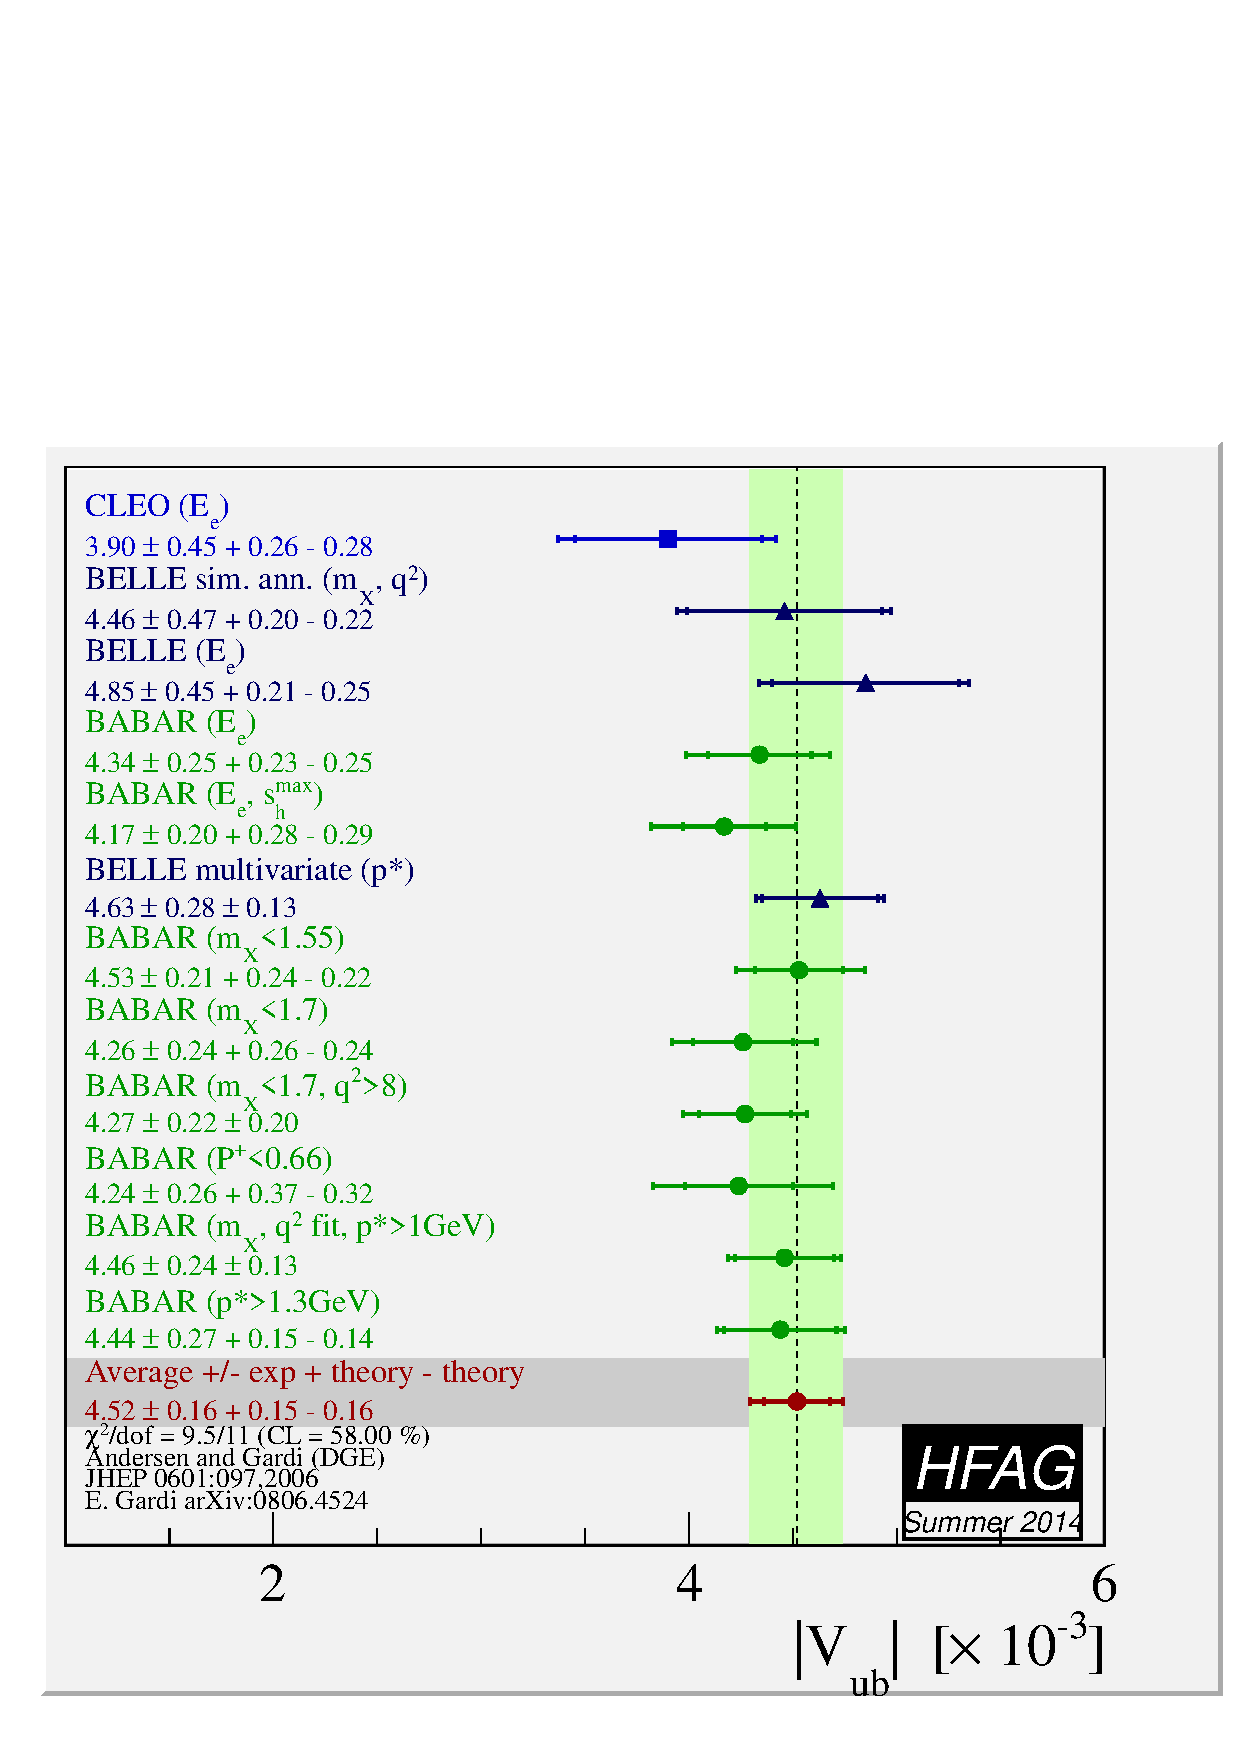
\includegraphics[width=0.48\textwidth]{figures/slb/vub_clnu_mc_asym_DGE.pdf}
%\end{center}
%\caption{Measurements of $\vub$ from inclusive semileptonic decays 
%and their average based on the DGE prescription.
%``$E_e$'', ``$M_X$'', ``$(M_X,q^2)$'' `$P^+$'', ``$p^*$ and ``($E_e,s^{max}_h$)'' indicate the 
%analysis type and applied cut.}
%\label{fig:DGE}
%\end{figure}

\subsubsection{GGOU}
Gambino, Giordano, Ossola and Uraltsev (GGOU)~\cite{Gambino:2007rp} 
compute the triple differential decay rates of $B \to X_u \ell^+ \nul$, 
including all perturbative and non--perturbative effects through $O(\alphas^2 \beta_0)$ 
and $O(1/m_b^3)$. 
The Fermi motion is parameterized in terms of a single light--cone function 
for each structure function and for any value of $q^2$, accounting for all subleading effects. 
The calculations are performed in the kinetic scheme, a framework characterized by a Wilsonian 
treatment with a hard cutoff $\mu \sim 1 $ GeV.
GGOU have not included calculations for the ``($E_e,s^{max}_h$)'' analysis. 
The heavy quark parameters determined  
from the global fit in the kinetic scheme, described in \ref{globalfitsKinetic}, are used as inputs: 
$m_b(kin)=(4.541 \pm 0.023)$ GeV, 
$\mu_\pi^2(kin)=(0.414 \pm 0.078)$ GeV$^2$. 
The extracted values
of \vub\, for each measurement along with their average are given in
Table~\ref{tab:bulnu} and illustrated in Figure~\ref{fig:GGOU_ADFR}(a).
The total error is $^{+4.3}_{-4.8}\%$ whose breakdown is:
statistics ($^{+1.9}_{-1.9}\%$),
detector ($^{+1.7}_{-1.7}\%$),
$B\to X_c \ell^+ \nul$ model ($^{+1.3}_{-1.3}\%$),
$B\to X_u \ell^+ \nul$ model ($^{+1.9}_{-1.9}\%$),
$\alpha_s$, $m_b$ and other non--perturbative parameters ($^{+1.6}_{-1.6}\%$), 
higher order perturbative and non--perturbative corrections ($^{+1.5}_{-1.5}\%$), 
modelling of the $q^2$ tail and choice of the scale $q^{2*}$ ($^{+1.4}_{-1.4}\%$), 
weak annihilations matrix element ($^{+0.0}_{-2.0}\%$), 
functional form of the distribution functions ($^{+0.2}_{-0.2}\%$), 
The leading uncertainties
on  \vub\ are both from theory, and are due to perturbative and non--perturbative
parameters and the modelling of the $q^2$ tail and choice of the scale $q^{2*}$. 
The uncertainty due to 
weak annihilation has been assumed to be asymmetric, i.e. it only tends to decrease \vub.

%\begin{figure}
%\begin{center}
%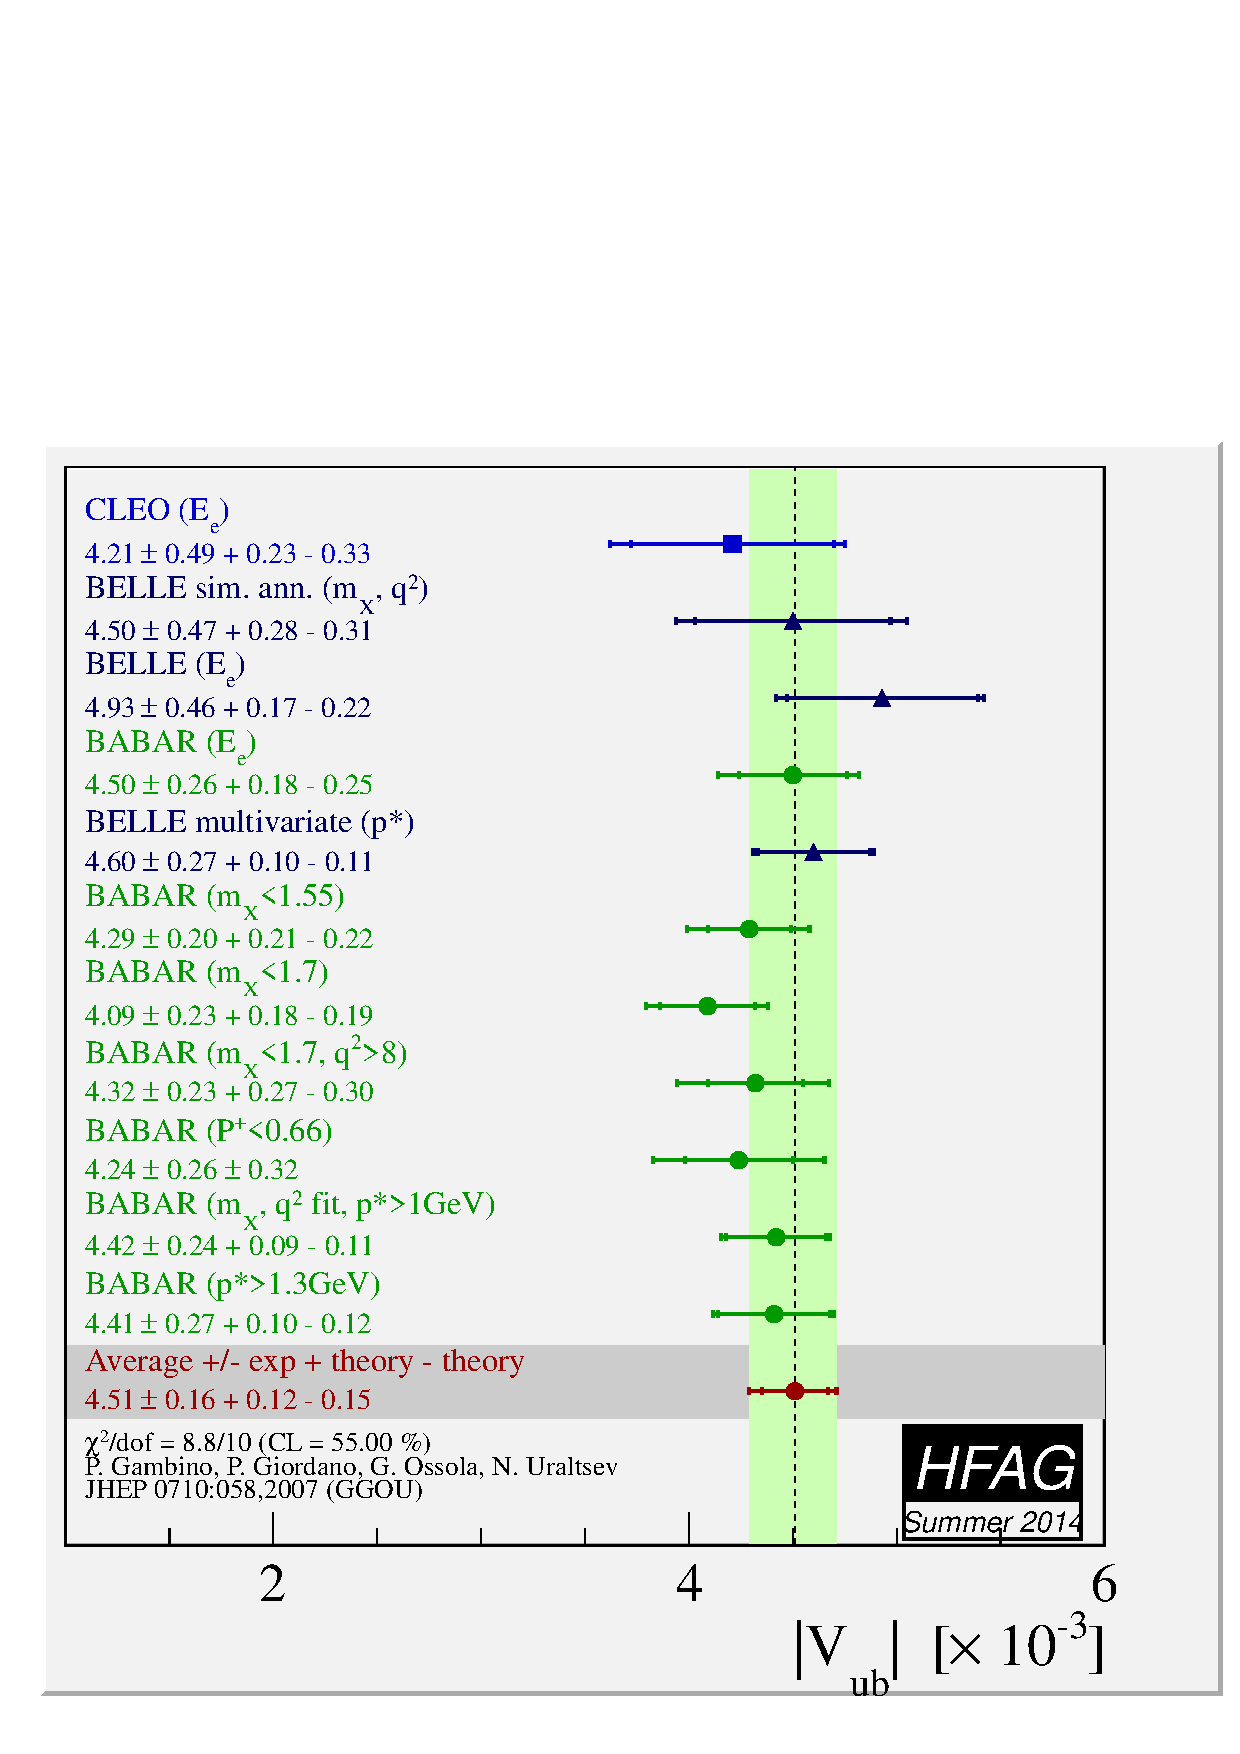
\includegraphics[width=0.48\textwidth]{figures/slb/vub_clnu_mc_GGOU.pdf}
%\end{center}
%\caption{Measurements of $\vub$ from inclusive semileptonic decays 
%and their average based on the GGOU prescription.
%``$E_e$'', ``$M_X$'', ``$(M_X,q^2)$'' `$P^+$'', ``$p^*$ and ``($E_e,s^{max}_h$)''  indicate the
%analysis type and applied cut.}
%\label{fig:GGOU}
%\end{figure}

\subsubsection{ADFR}
Aglietti, Di Lodovico, Ferrera and Ricciardi (ADFR)~\cite{Aglietti:2007ik}
use an approach to extract \vub, which makes use of the ratio
of the  $B \to X_c \ell^+ \nul$ and $B \to X_u \ell^+ \nul$ widths. 
The normalized triple differential decay rate for 
$B \to X_u \ell^+ \nul$~\cite{Aglietti:2006yb,Aglietti:2005mb, Aglietti:2005bm, Aglietti:2005eq}
is calculated with a model based on (i) soft--gluon resummation 
to next--to--next--leading order and (ii) an effective QCD coupling without
Landau pole. This coupling is constructed by means of an extrapolation to low
energy of the high--energy behaviour of the standard coupling. More technically,
an analyticity principle is used.
The lower cut on the electron energy for the endpoint analyses is 2.3~GeV~\cite{Aglietti:2006yb}.
The ADFR calculation uses the $\overline{MS}$ renormalization scheme; the heavy quark parameters determined  
from the global fit in the kinetic scheme, described in \ref{globalfitsKinetic}, were therefore 
translated into the $\overline{MS}$ scheme by using a calculation by Gardi, giving 
$m_b({\overline{MS}})=(4.177 \pm 0.043)$ GeV.
The extracted values
of \vub\, for each measurement along with their average are given in
Table~\ref{tab:bulnu} and illustrated in Figure~\ref{fig:GGOU_ADFR}(b).
The total error is $^{+5.4}_{-5.3}\%$ whose breakdown is:
statistics ($^{+1.8}_{-1.8}\%$),
detector ($^{+1.8}_{-2.0}\%$),
$B\to X_c \ell^+ \nul$ model ($^{+1.4}_{-1.4}\%$),
$B\to X_u \ell^+ \nul$ model ($^{+1.3}_{-1.3}\%$),
$\alpha_s$ ($^{+1.1}_{-1.0}\%$), 
$|V_{cb}|$ ($^{+2.0}_{-2.0}\%$), 
$m_b$ ($^{+0.7}_{-0.7}\%$), 
$m_c$ ($^{+0.4}_{-0.7}\%$), 
semileptonic branching fraction ($^{+0.8}_{-0.7}\%$), 
theory model ($^{+3.5}_{-3.5}\%$).
The leading
uncertainty, from theory, is due to the theory model.

%\begin{figure}
%\begin{center}
%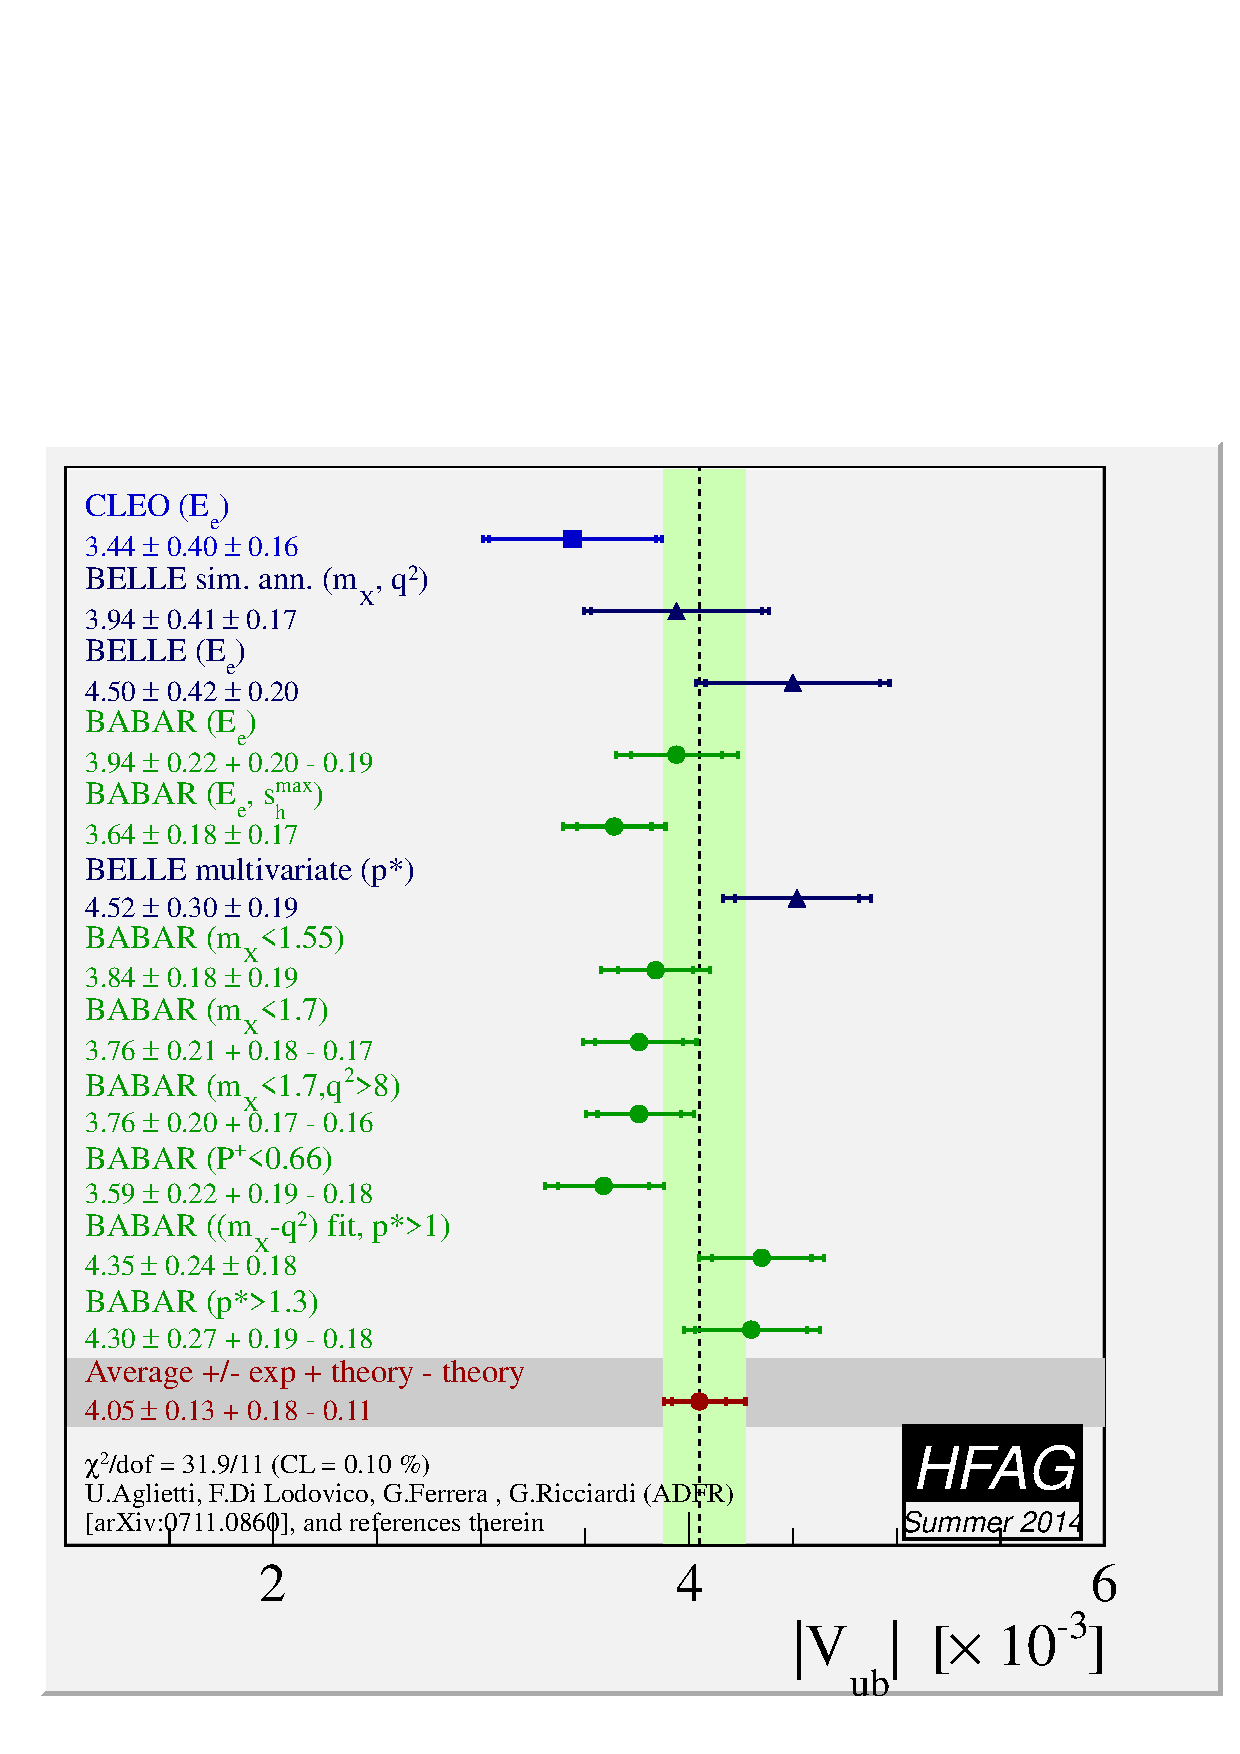
\includegraphics[width=0.48\textwidth]{figures/slb/vub_clnu_mc_ADFR.pdf}
%\end{center}
%\caption{Measurements of $\vub$ from inclusive semileptonic decays 
%and their average based on the ADFR prescription.
%``$E_e$'', ``$M_X$'', ``$(M_X,q^2)$'' `$P^+$'', ``$p^*$ and ``($E_e,s^{max}_h$)'' indicate the 
%analysis type and applied cut.}
%\label{fig:AC}
%\end{figure}

\subsubsection{BLL}
Bauer, Ligeti, and Luke (BLL)~\cite{ref:BLL} give a
HQET-based prescription that advocates combined cuts on the dilepton invariant mass, $q^2$,
and hadronic mass, $m_X$, to minimise the overall uncertainty on \vub.
In their reckoning a cut on $m_X$ only, although most efficient at
preserving phase space ($\sim$80\%), makes the calculation of the partial
rate untenable due to uncalculable corrections
to the $b$-quark distribution function or shape function. These corrections are
suppressed if events in the low $q^2$ region are removed. The cut combination used
in measurements is $M_x<1.7$ GeV/$c^2$ and $q^2 > 8$ GeV$^2$/$c^2$.  
The extracted values
of \vub\, for each measurement along with their average are given in
Table~\ref{tab:bulnu} and illustrated in Figure~\ref{fig:BLL}.
The total error is $^{+7.7}_{-7.7}\%$ whose breakdown is:
statistics ($^{+3.3}_{-3.3}\%$),
detector ($^{+3.0}_{-3.0}\%$),
$B\to X_c \ell^+ \nul$ model ($^{+1.6}_{-1.6}\%$),
$B\to X_u \ell^+ \nul$ model ($^{+1.1}_{-1.1}\%$),
spectral fraction ($m_b$) ($^{+3.0}_{-3.0}\%$),
perturbative : strong coupling $\alpha_s$ ($^{+3.0}_{-3.0}\%$),
residual shape function ($^{+2.5}_{-2.5}\%$),
third order terms in the OPE ($^{+4.0}_{-4.0}\%$),
The leading
uncertainties, both from theory, are due to residual shape function
effects and third order terms in the OPE expansion. The leading
experimental uncertainty is due to statistics. 

\begin{figure}
\begin{center}
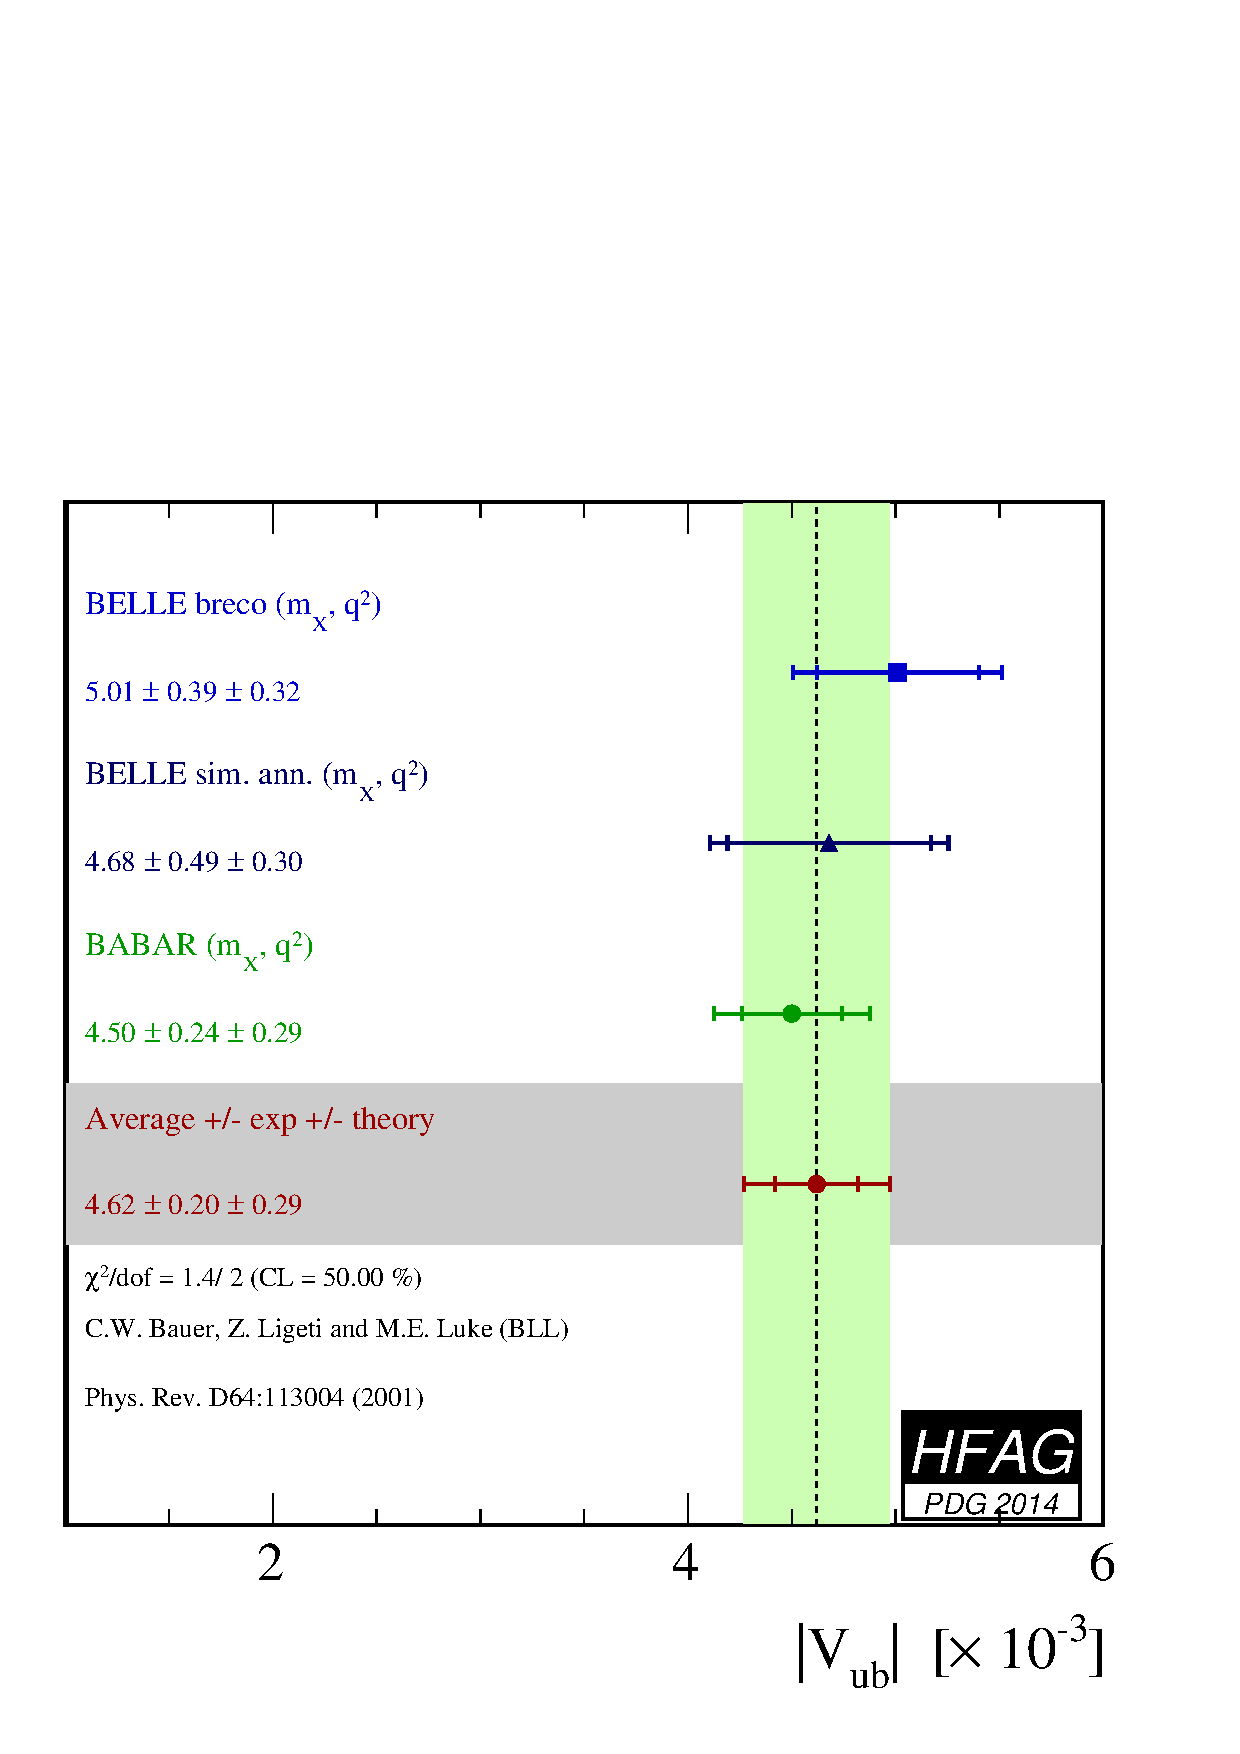
\includegraphics[width=0.48\textwidth]{figures/slb/vub_mxq2_allMoments.pdf}
\end{center}
\caption{Measurements of $\vub$ from inclusive semileptonic decays 
and their average in the BLL prescription.
``$(M_X, q^2)$'' indicates the analysis type.}
\label{fig:BLL}
\end{figure}


\subsubsection{Summary}
A summary of the averages presented in several different
frameworks and results by V.B.~Golubev, V.G.~Luth and Yu.I.~Skovpen~\cite{Golubev:2007cs},
based on prescriptions by LLR~\cite{Leibovich:1999xf} and LNP~\cite{Lange:2005qn} 
to reduce the leading shape function uncertainties are presented in 
Table~\ref{tab:vubcomparison}.
A value judgement based on a direct comparison should be
avoided at the moment, experimental and theoretical uncertainties play out
differently between the schemes and the theoretical assumptions for the
theory calculations are different.

\input{tables/slb/vubcomparison.tex}





%
% ======================================================================
%

% ======================================================================

%\cleardoublepage

\section{Semileptonic $B$ decays}
\label{sec:slbdecays}

This section contains our averages for semileptonic $B$~meson decays,
{\it i.e.}, decays of the type $B\to X\ell\nu_\ell$, where $X$ is a
hadronic system, $\ell$ a charged lepton and $\nu_\ell$ its corresponding
neutrino. Unless otherwise stated, $\ell$ stands for an electron
\emph{or} a muon, lepton universality is assumed, and both charge
conjugate states are included. Some averages assume isospin symmetry
and this will be explicitly mentioned at every instance.

The averages are organized by the flavour changing transition
(the CKM-favoured $b\to c$ transition and the CKM-suppressed $b\to u$
transition) and by the experimental definition of the hadronic
$X$~system. Measurements which are sensitive to only a specific
hadronic state ($X=D,D^*,\pi,\dots$) are called \emph{exclusive} while
analyses that measure all hadronic states within a given region of
phase space are \emph{inclusive}. The principal reason why semileptonic
$B$~decays are studied in experiments is the determination of the CKM
matrix element magnitudes $|V_{cb}|$ and $|V_{ub}|$. The averages in
the different subsections thus focus very much on these two
fundamental parameters of the Standard Model. In the last subsection,
we discuss semileptonic $B$~decays with a $\tau$-lepton. These
decays are relevant to the search for physics beyond the Standard
Model, {\it e.g.}, in the context of the type II
Two-Higgs-Doublet-Model (2HDM).

The technique for obtaining the averages follows the general HFAG
procedure (Sect.~\ref{sec:method}) unless otherwise stated. More
information on the averages, in particular the common input parameters
is available on the HFAG semileptonic webpage:

\centerline{\tt http://www.slac.stanford.edu/xorg/hfag/semi/pdg14/}

% ======================================================================

%% \clearpage

% ======================================================================
% Common set of input parameters

%%%commented out 2-Aug-2010 by AJS
%%%\input{slbdecays/common.tex}

% ======================================================================
% Exclusive CKM-favoured decays
% -- \include{b2cexcl.tex}
% ======================================================================
\subsection{Exclusive CKM-favoured decays}
\label{slbdecays_b2cexcl}
% -------------------------------------------
This section is organized as follows: First, we present averages for
the decays $\bar B\to D^*\ell^-\bar\nu_\ell$ and $\bar B\to
D\ell^-\bar\nu_\ell$. In addition to the branching fractions, the CKM
element $|V_{cb}|$ is extracted. We then provide
averages for the inclusive branching fractions $\cbf(\bar B\to
D^{(*)}\pi \ell^-\bar\nu_\ell)$ and for $B$ semileptonic decays into
orbitally-excited $P$-wave charm mesons ($D^{**}$). As the $D^{**}$
branching fraction is poorly known, we report the averages for the products 
$\cbf(B^-\to D^{**}(D^{(*)}\pi)\ell^-\bar\nu_\ell)\times
\cbf(D^{**}\to D^{(*)}\pi)$.

%===================================================================
% D and D* 
%===================================================================

\mysubsubsection{$\bar B\to D^*\ell^-\bar\nu_\ell$}
\label{slbdecays_dstarlnu}

The kinematics of the decay $\bar B\to D^*\ell^-\bar\nu_\ell$ are
described by the form factor $\eta_\mathrm{EW}{\cal F}(w)$, where
$\eta_{EW}$ is a known electro-weak correction factor and $w$ is the
product of the $B$ and $D^*$ meson 4-velocities, $w=v_B\cdot
v_{D^*}$. Most experiments use the parameterization of Caprini,
Lellouch and Neubert (CLN) to describe the shape and normalization of
$\eta_\mathrm{EW}{\cal F}(w)$ by four quantities:
$\eta_\mathrm{EW}{\cal F}(1)\vcb$, $\rho^2$, $R_1(1)$ and
$R_2(1)$~\cite{CLN}. Our main average and the determination of $\vcb$
are based on this parameterization.

We use the measurements of these form factor parameters shown in
Table~\ref{tab:vcbf1} and rescale them to the latest values of the
input parameters (mainly branching fractions of charmed
mesons)~\cite{HFAG_sl:inputparams}. Most of the measurements in
Table~\ref{tab:vcbf1} are based exclusively on the decay $\bar B^0\to
D^{*+}\ell^-\bar\nu_\ell$. Some
measurements~\cite{Adam:2002uw,Aubert:2009_1} are sensitive also to
$B^-\to D^{*0}\ell^-\bar\nu_\ell$ and one
measurement~\cite{Aubert:2009_3} is based exclusively on the decay
$B^-\to D^{*0}\ell^-\bar\nu_\ell$. Our analysis thus assumes isospin
symmetry.
% ----------------------------------------------------------------------
\begin{table}[!htb]
\caption{Measurements of the Caprini, Lellouch and Neubert
  (CLN)~\cite{CLN} form factor parameters in $\bar B\to
  D^*\ell^-\bar\nu_\ell$ before and after rescaling. Most analyses
  (except \cite{Dungel:2010uk,Aubert:2006mb}) measure only
  $\eta_\mathrm{EW}{\cal F}(1)\vcb$, and $\rho^2$, so only these two
  parameters are shown here. The average is the result of a
  4-dimensional fit to the rescaled measurements of
  $\eta_\mathrm{EW}{\cal F}(1)\vcb$, $\rho^2$, $R_1(1)$ and
  $R_2(1)$ -- see the text for more details. The $\chi^2$~value of the
  combination is 30.0 for 23 degrees of freedom (CL=$15.0\%$).}
\begin{center}
\resizebox{0.99\textwidth}{!}{
\begin{tabular}{|l|c|c|}
  \hline
  Experiment
  & $\eta_\mathrm{EW}{\cal F}(1)\vcb [10^{-3}]$ (rescaled)
  & $\rho^2$ (rescaled)\\
  & $\eta_\mathrm{EW}{\cal F}(1)\vcb [10^{-3}]$ (published)
  & $\rho^2$ (published)\\
  \hline\hline
  ALEPH~\cite{Buskulic:1996yq}
  & $31.23\pm 1.80_{\rm stat}\pm 1.30_{\rm syst}$
  & $0.493\pm 0.228_{\rm stat}\pm 0.144_{\rm syst}$\\
  & $31.9\pm 1.8_{\rm stat}\pm 1.9_{\rm syst}$
  & $0.37\pm 0.26_{\rm stat}\pm 0.14_{\rm syst}$\\
  \hline
  CLEO~\cite{Adam:2002uw}
  & $39.94\pm 1.23_{\rm stat}\pm 1.62_{\rm syst}$
  & $1.367\pm 0.085_{\rm stat}\pm 0.086_{\rm syst}$\\
  & $43.1\pm 1.3_{\rm stat}\pm 1.8_{\rm syst}$
  & $1.61\pm 0.09_{\rm stat}\pm 0.21_{\rm syst}$\\
  \hline
  OPAL excl~\cite{Abbiendi:2000hk}
  & $36.50\pm 1.60_{\rm stat}\pm 1.49_{\rm syst}$
  & $1.234\pm 0.212_{\rm stat}\pm 0.145_{\rm syst}$\\
  & $36.8\pm 1.6_{\rm stat}\pm 2.0_{\rm syst}$
  & $1.31\pm 0.21_{\rm stat}\pm 0.16_{\rm syst}$\\
  \hline
  OPAL partial reco~\cite{Abbiendi:2000hk}
  & $37.14\pm 1.19_{\rm stat}\pm 2.36_{\rm syst}$
  & $1.152\pm 0.145_{\rm stat}\pm 0.294_{\rm syst}$\\
  & $37.5\pm 1.2_{\rm stat}\pm 2.5_{\rm syst}$
  & $1.12\pm 0.14_{\rm stat}\pm 0.29_{\rm syst}$\\
  \hline
  DELPHI partial reco~\cite{Abreu:2001ic}
  & $35.32\pm 1.40_{\rm stat}\pm 2.33_{\rm syst}$
  & $1.174\pm 0.126_{\rm stat} \pm 0.377_{\rm syst}$\\
  & $35.5\pm 1.4_{\rm stat}\ {}^{+2.3}_{-2.4}{}_{\rm syst}$
  & $1.34\pm 0.14_{\rm stat}\ {}^{+0.24}_{-0.22}{}_{\rm syst}$\\
  \hline
  DELPHI excl~\cite{Abdallah:2004rz}
  & $36.10\pm 1.70_{\rm stat}\pm 1.97_{\rm syst}$
  & $1.081\pm 0.142_{\rm stat} \pm 0.152_{\rm syst}$\\
  & $39.2\pm 1.8_{\rm stat}\pm 2.3_{\rm syst}$
  & $1.32\pm 0.15_{\rm stat}\pm 0.33_{\rm syst}$\\
  \hline
  \belle~\cite{Dungel:2010uk}
  & $34.60\pm 0.17_{\rm stat}\pm 1.02_{\rm syst}$
  & $1.212\pm 0.034_{\rm stat}\pm 0.009_{\rm syst}$\\
  & $34.6\pm 0.2_{\rm stat}\pm 1.0_{\rm syst}$
  & $1.214\pm 0.034_{\rm stat} \pm 0.009_{\rm syst}$\\
  \hline
  \babar\ excl~\cite{Aubert:2006mb}
  & $33.94\pm 0.30_{\rm stat}\pm 0.99_{\rm syst}$
  & $1.185\pm 0.048_{\rm stat}\pm 0.029_{\rm syst}$\\
  & $34.7\pm 0.3_{\rm stat}\pm 1.1_{\rm syst}$
  & $1.18\pm 0.05_{\rm stat}\pm 0.03_{\rm syst}$\\
  \hline
  \babar\ $D^{*0}$~\cite{Aubert:2009_3}
  & $35.22\pm 0.59_{\rm stat}\pm 1.33_{\rm syst}$
  & $1.128\pm 0.058_{\rm stat}\pm 0.055_{\rm syst}$\\
  & $35.9\pm 0.6_{\rm stat}\pm 1.4_{\rm syst}$
  & $1.16\pm 0.06_{\rm stat}\pm 0.08_{\rm syst}$\\
  \hline
  \babar\ global fit~\cite{Aubert:2009_1}
  & $35.76\pm 0.20_{\rm stat}\pm 1.10_{\rm syst}$
  & $1.193\pm 0.020_{\rm stat}\pm 0.061_{\rm syst}$\\
  & $35.7\pm 0.2_{\rm stat}\pm 1.2_{\rm syst}$
  & $1.21\pm 0.02_{\rm stat}\pm 0.07_{\rm syst}$\\
  \hline
  {\bf Average}
  & \mathversion{bold} $35.81\pm 0.11_{\rm stat}\pm 0.44_{\rm syst}$ &
  \mathversion{bold} $1.207\pm 0.015_{\rm stat}\pm 0.021_{\rm syst}$\\
  \hline 
\end{tabular}
}
\end{center}
\label{tab:vcbf1}
\end{table}
% ----------------------------------------------------------------------


In the next step, we perform a four-dimensional fit of the parameters
$\eta_\mathrm{EW}{\cal F}(1)\vcb$, $\rho^2$, $R_1(1)$ and $R_2(1)$
using the rescaled measurements and taking into account correlated
statistical and systematic uncertainties. Only two measurements
constrain all four parameters~\cite{Dungel:2010uk,Aubert:2006mb}, the remaining
measurements determine only the normalization $\eta_\mathrm{EW}{\cal
  F}(1)\vcb$ and the slope $\rho^2$. The result of the fit is
\begin{eqnarray}
  \eta_\mathrm{EW}{\cal F}(1)\vcb & = & (35.81\pm 0.45)\times
  10^{-3}~, \label{eq:vcbf1} \\
  \rho^2 & = & 1.207\pm 0.026~,\\
  R_1(1) & = & 1.406\pm 0.033~, \label{eq:r1} \\
  R_2(1) & = & 0.853\pm 0.020~, \label{eq:r2}
\end{eqnarray}
and the correlation coefficients are
\begin{eqnarray}
  \rho_{\eta_\mathrm{EW}{\cal F}(1)\vcb,\rho^2} & = & 0.323~,\\
  \rho_{\eta_\mathrm{EW}{\cal F}(1)\vcb,R_1(1)} & = & -0.108~,\\
  \rho_{\eta_\mathrm{EW}{\cal F}(1)\vcb,R_2(1)} & = & -0.063~,\\
  \rho_{\rho^2,R_1(1)} & = & 0.568~,\\
  \rho_{\rho^2,R_2(1)} & = & -0.809~,\\
  \rho_{R_1(1),R_2(1)} & = & -0.758~.
\end{eqnarray}
The uncertainties and correlations quoted here include both
statistical and systematic contributions. The $\chi^2$ of the fit is
30.0 for 23 degrees of freedom, which corresponds to a confidence
level of 15.0\%. An illustration of this fit result is given in
Fig.~\ref{fig:vcbf1}.
\begin{figure}[!ht]
  \begin{center}
  \unitlength 1.0cm % coordinates in cm
  \begin{picture}(14.,8.0)
    \put(  8.0,
    -0.2){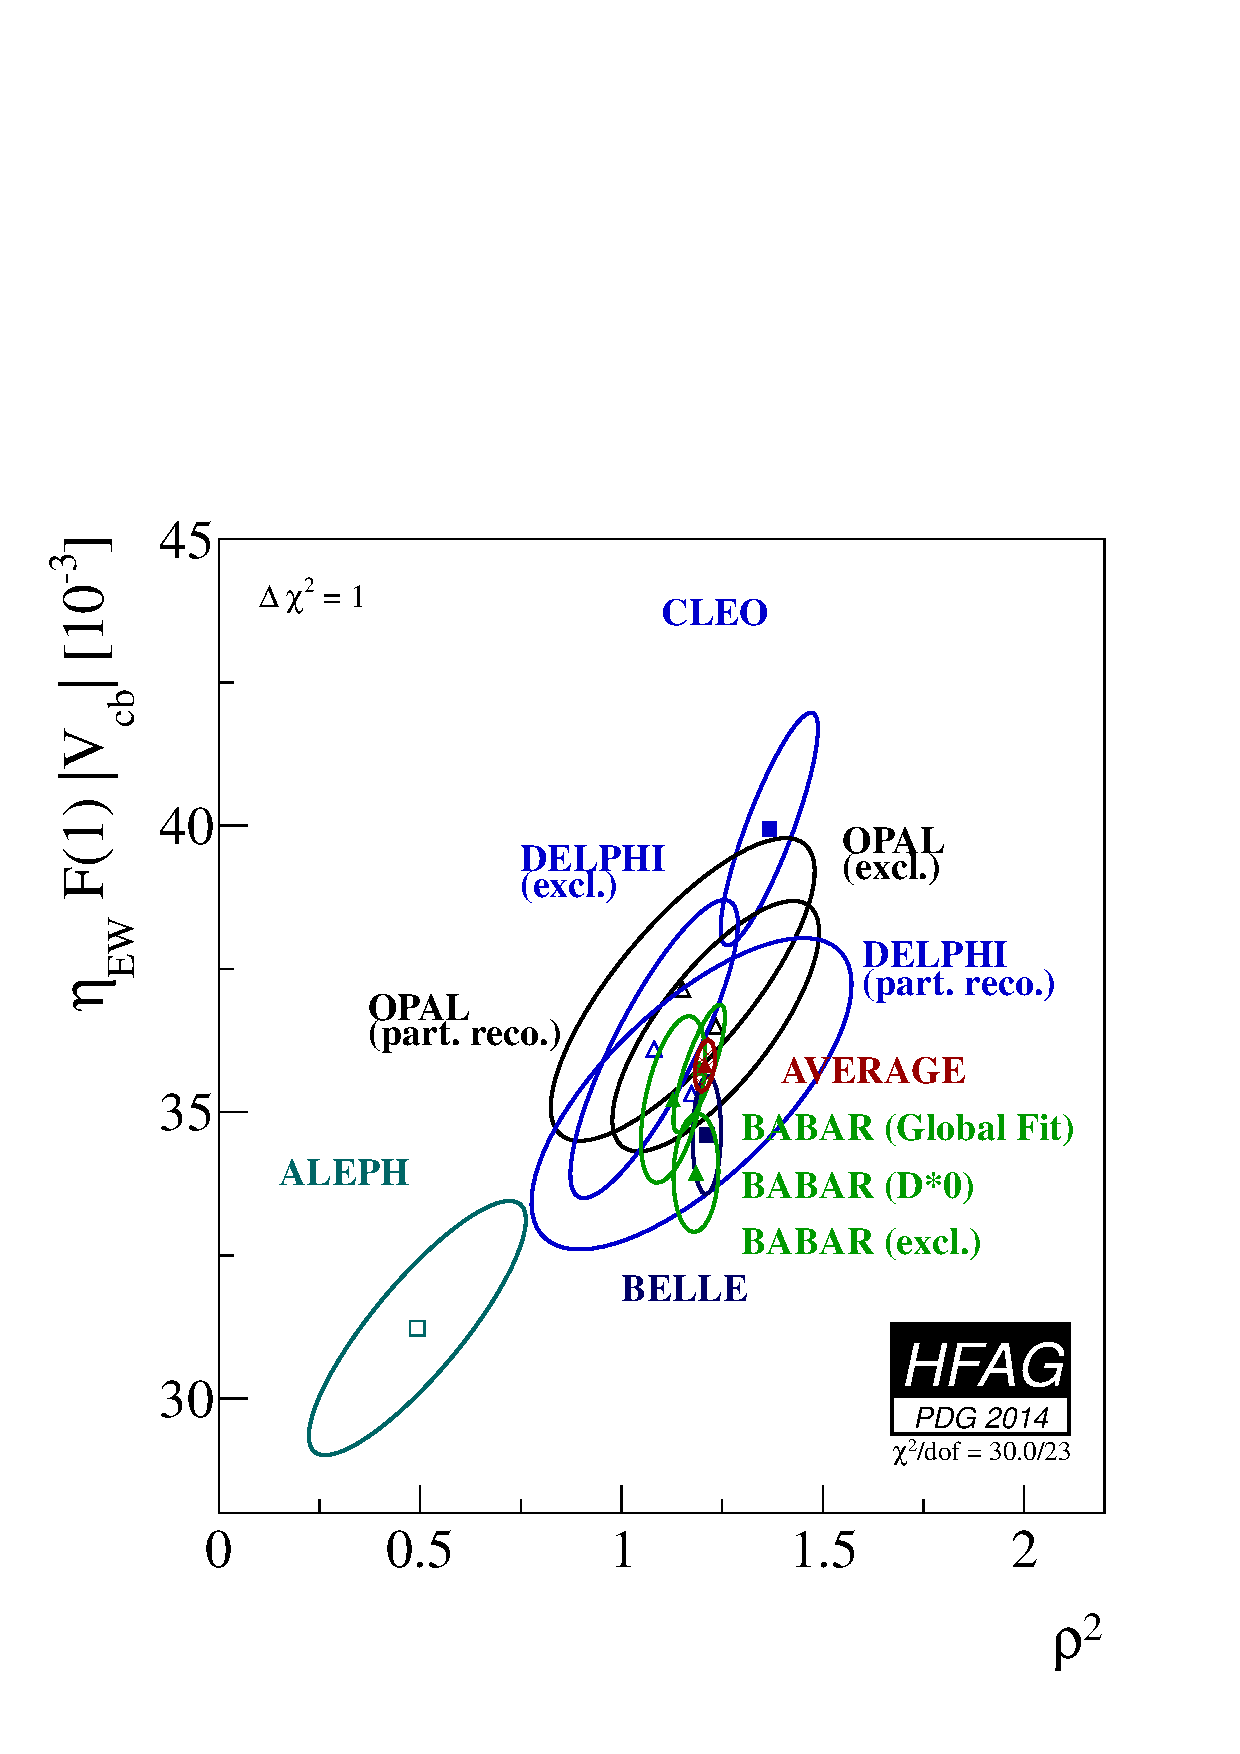
\includegraphics[width=8.0cm]{figures/slb/vcbf1_vs_rho2.pdf}
    }
    \put( -0.5,
    0.0){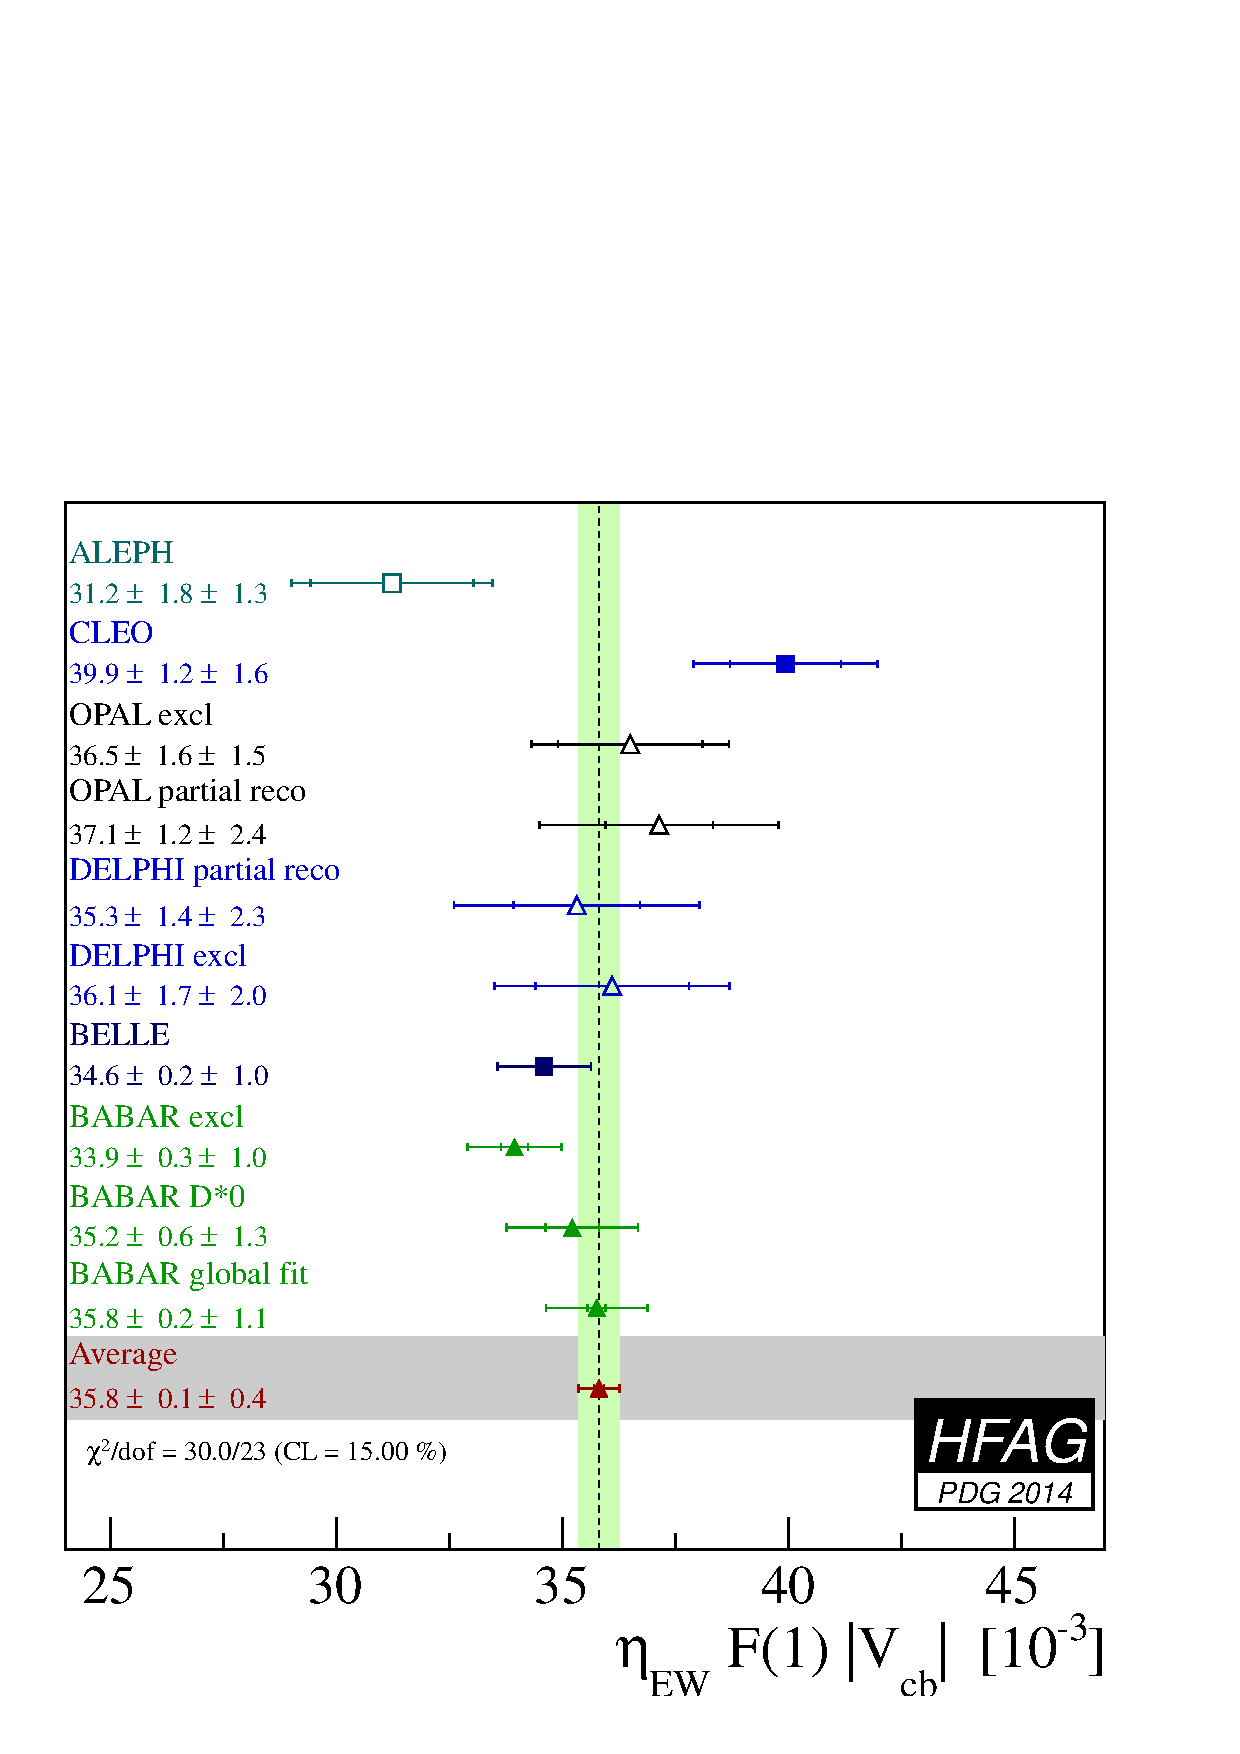
\includegraphics[width=7.5cm]{figures/slb/vcbf1.pdf}
    }
    \put(  5.5,  6.8){{\large\bf a)}}  
    \put( 14.4,  6.8){{\large\bf b)}}
  \end{picture}
  \caption{(a) Illustration of the $\eta_\mathrm{EW}{\cal F}(1)\vcb$
      average. (b) Illustration of the $\eta_\mathrm{EW}{\cal
        F}(1)\vcb$ vs.\ $\rho^2$ average. The error ellipses
      correspond  to $\Delta\chi^2 = 1$ (CL=39\%).} \label{fig:vcbf1}
  \end{center}
\end{figure}

Using the lastest update from the FNAL/MILC
group~\cite{Bailey:2014tva}, the form factor normalization
$\eta_\mathrm{EW}{\cal F}(1)$ is
\begin{equation}
  \eta_\mathrm{EW}{\cal F}(1) = 0.920\pm 0.014~,
\end{equation}
which results in the following determination of $\vcb$ from
Eq.~\ref{eq:vcbf1},
\begin{equation}
  \vcb = (38.94\pm 0.49_{\rm exp}\pm 0.58_{\rm th})\times
  10^{-3}~, \label{eq:vcbdstar}
\end{equation}
where the first uncertainty is experimental and the second error is
theoretical (lattice QCD calculation and electro-weak correction).

From each rescaled measurement in Table~\ref{tab:vcbf1}, we
calculate the $\bar B\to D^*\ell^-\bar\nu_\ell$ form factor
$\eta_\mathrm{EW}{\cal F}(w)$ and, by numerical integration, the
branching ratio of the decay $\bar B^0\to
D^{*+}\ell^-\bar\nu_\ell$. For measurements which do not determine the
parameters $R_1(1)$ and $R_2(1)$ we assume the average
values~Eqs.~\ref{eq:r1} and \ref{eq:r2}. The results are quoted in
Table~\ref{tab:dstarlnu}. The branching ratio found for the average
values of $\eta_\mathrm{EW}{\cal F}(1)\vcb$, $\rho^2$, $R_1(1)$ and
$R_2(1)$ is
\begin{equation}
  \cbf(\BzbDstarlnu)=(4.93\pm 0.11)\%~.
\end{equation}

To test isospin symmetry, we have performed a simple 1-dimensional
average of measurements sensitive to the decay $B^-\to
D^{*0}\ell^-\bar\nu_\ell$ only, which is shown in
Table~\ref{tab:dstar0lnu}. Fig.~\ref{fig:brdsl} illustrates our two
averages of $\bar B\to D^*\ell^-\bar\nu_\ell$.
% ----------------------------------------------------------------------
\begin{table}[!htb]
\caption{$\BzbDstarlnu$ branching fractions calculated from the
  rescaled measurements in Table~\ref{tab:vcbf1}, asumming the CLN
  parameterization of the form factor~\cite{CLN}. The branching ratios
  published in Refs.~\cite{Aubert:2009_3,Aubert:2009_1} have been
  rescaled by the factor $\tau(B^0)/\tau(B^+)$. While the fit assumes
  isospin symmetry, most measurements included here use only the decay
  $\BzbDstarlnu$.}
\begin{center} 
\resizebox{0.99\textwidth}{!}{
\begin{tabular}{|l|c|c|}\hline
  Experiment & $\cbf(\BzbDstarlnu)$ [\%] (calculated) &
  $\cbf(\BzbDstarlnu)$ [\%] (published)\\
  \hline\hline
  ALEPH~\hfill\cite{Buskulic:1996yq}
  & $5.35\pm 0.25_{\rm stat} \pm 0.31_{\rm syst}$
  & $5.53\pm 0.26_{\rm stat} \pm 0.52_{\rm syst}$\\
  CLEO~\hfill\cite{Adam:2002uw}
  & $5.62\pm 0.18_{\rm stat} \pm 0.26_{\rm syst}$
  & $6.09\pm 0.19_{\rm stat} \pm 0.40_{\rm syst}$\\
  OPAL excl~\hfill\cite{Abbiendi:2000hk}
  & $5.05\pm 0.19_{\rm stat} \pm 0.42_{\rm syst}$
  & $5.11\pm 0.19_{\rm stat} \pm 0.49_{\rm syst}$\\
  OPAL partial reco~\hfill\cite{Abbiendi:2000hk}
  & $5.46\pm 0.25_{\rm stat} \pm 0.52_{\rm syst}$
  & $5.92\pm 0.27_{\rm stat} \pm 0.68_{\rm syst}$\\
  DELPHI partial reco~\hfill\cite{Abreu:2001ic}
  & $4.88\pm 0.13_{\rm stat} \pm 0.72_{\rm syst}$
  & $4.70\pm 0.13_{\rm stat} \ {}^{+0.36}_{-0.31}\ {}_{\rm syst}$\\
  DELPHI excl~\hfill\cite{Abdallah:2004rz}
  & $5.35\pm 0.20_{\rm stat} \pm 0.37_{\rm syst}$
  & $5.90\pm 0.22_{\rm stat} \pm 0.50_{\rm syst}$\\
  \belle~\hfill\cite{Dungel:2010uk}
  & $4.56\pm 0.03_{\rm stat} \pm 0.26_{\rm syst}$
  & $4.58\pm 0.03_{\rm stat} \pm 0.26_{\rm syst}$\\
  \babar\ excl~\hfill\cite{Aubert:2006mb}
  & $4.54\pm 0.04_{\rm stat}\pm 0.25_{\rm syst}$
  & $4.69\pm 0.04_{\rm stat} \pm 0.34_{\rm syst}$\\
  \babar\ $D^{*0}$~\hfill\cite{Aubert:2009_3}
  & $4.97\pm 0.07_{\rm stat}\pm 0.34_{\rm syst}$
  & $5.15\pm 0.07_{\rm stat} \pm 0.38_{\rm syst}$\\
  \babar\ global fit~\hfill\cite{Aubert:2009_1}
  & $4.95\pm 0.02_{\rm stat}\pm 0.20_{\rm syst}$
  & $5.00\pm 0.02_{\rm stat} \pm 0.19_{\rm syst}$\\
  \hline 
  {\bf Average} & \mathversion{bold}$4.93\pm 0.01_{\rm stat}\pm
  0.11_{\rm syst}$ & \mathversion{bold}$\chi^2/\dof = 30.0/23$ (CL=$15.0\%$)\\
  \hline 
\end{tabular}
}
\end{center}
\label{tab:dstarlnu}
\end{table}
% ----------------------------------------------------------------------

% ----------------------------------------------------------------------0
\begin{table}[!htb]
\caption{Average of the $B^-\to D^{*0}\ell^-\bar\nu_\ell$ branching
  fraction measurements. This fit uses only measurements of $B^-\to
  D^{*0}\ell^-\bar\nu_\ell$.}
\begin{center}
\begin{tabular}{|l|c|c|}
  \hline
  Experiment & $\cbf(B^-\to D^{*0}\ell^-\bar\nu_\ell)$ [\%] (rescaled) &
  $\cbf(B^-\to D^{*0}\ell^-\bar\nu_\ell)$ [\%] (published)\\
  \hline \hline
  CLEO~\hfill\cite{Adam:2002uw}
  & $6.61\pm 0.20_{\rm stat}\pm 0.39_{\rm syst}$
  & $6.50\pm 0.20_{\rm stat}\pm 0.43_{\rm syst}$\\
  \babar tagged~\hfill\cite{Aubert:vcbExcl}
  & $5.72\pm 0.15_{\rm stat}\pm 0.30_{\rm syst}$
  & $5.83\pm 0.15_{\rm stat}\pm0.30_{\rm syst}$\\
  \babar~\hfill\cite{Aubert:2009_3}
  & $5.35\pm0.08_{\rm stat}\pm 0.40_{\rm syst}$
  & $5.56\pm0.08_{\rm stat} \pm0.41_{\rm syst}$\\
  \babar~\hfill\cite{Aubert:2009_1}
  & $5.43\pm 0.02_{\rm stat}\pm 0.21_{\rm syst}$
  & $5.40\pm 0.02_{\rm stat}\pm 0.21_{\rm syst}$\\
  \hline
  {\bf Average} & \mathversion{bold}$5.70\pm 0.02_{\rm stat}\pm
  0.19_{\rm syst}$ & \mathversion{bold}$\chi^2/\dof = 9.1/3$ (CL=$2.8\%$)\\
  \hline 
\end{tabular}
\end{center}
\label{tab:dstar0lnu}
\end{table}
% ----------------------------------------------------------------------

\begin{figure}[!ht]
  \begin{center}
  \unitlength1.0cm % coordinates in cm
  \begin{picture}(14.,8.0)  %ys(25.,6.0)
    \put( -0.5, 0.0){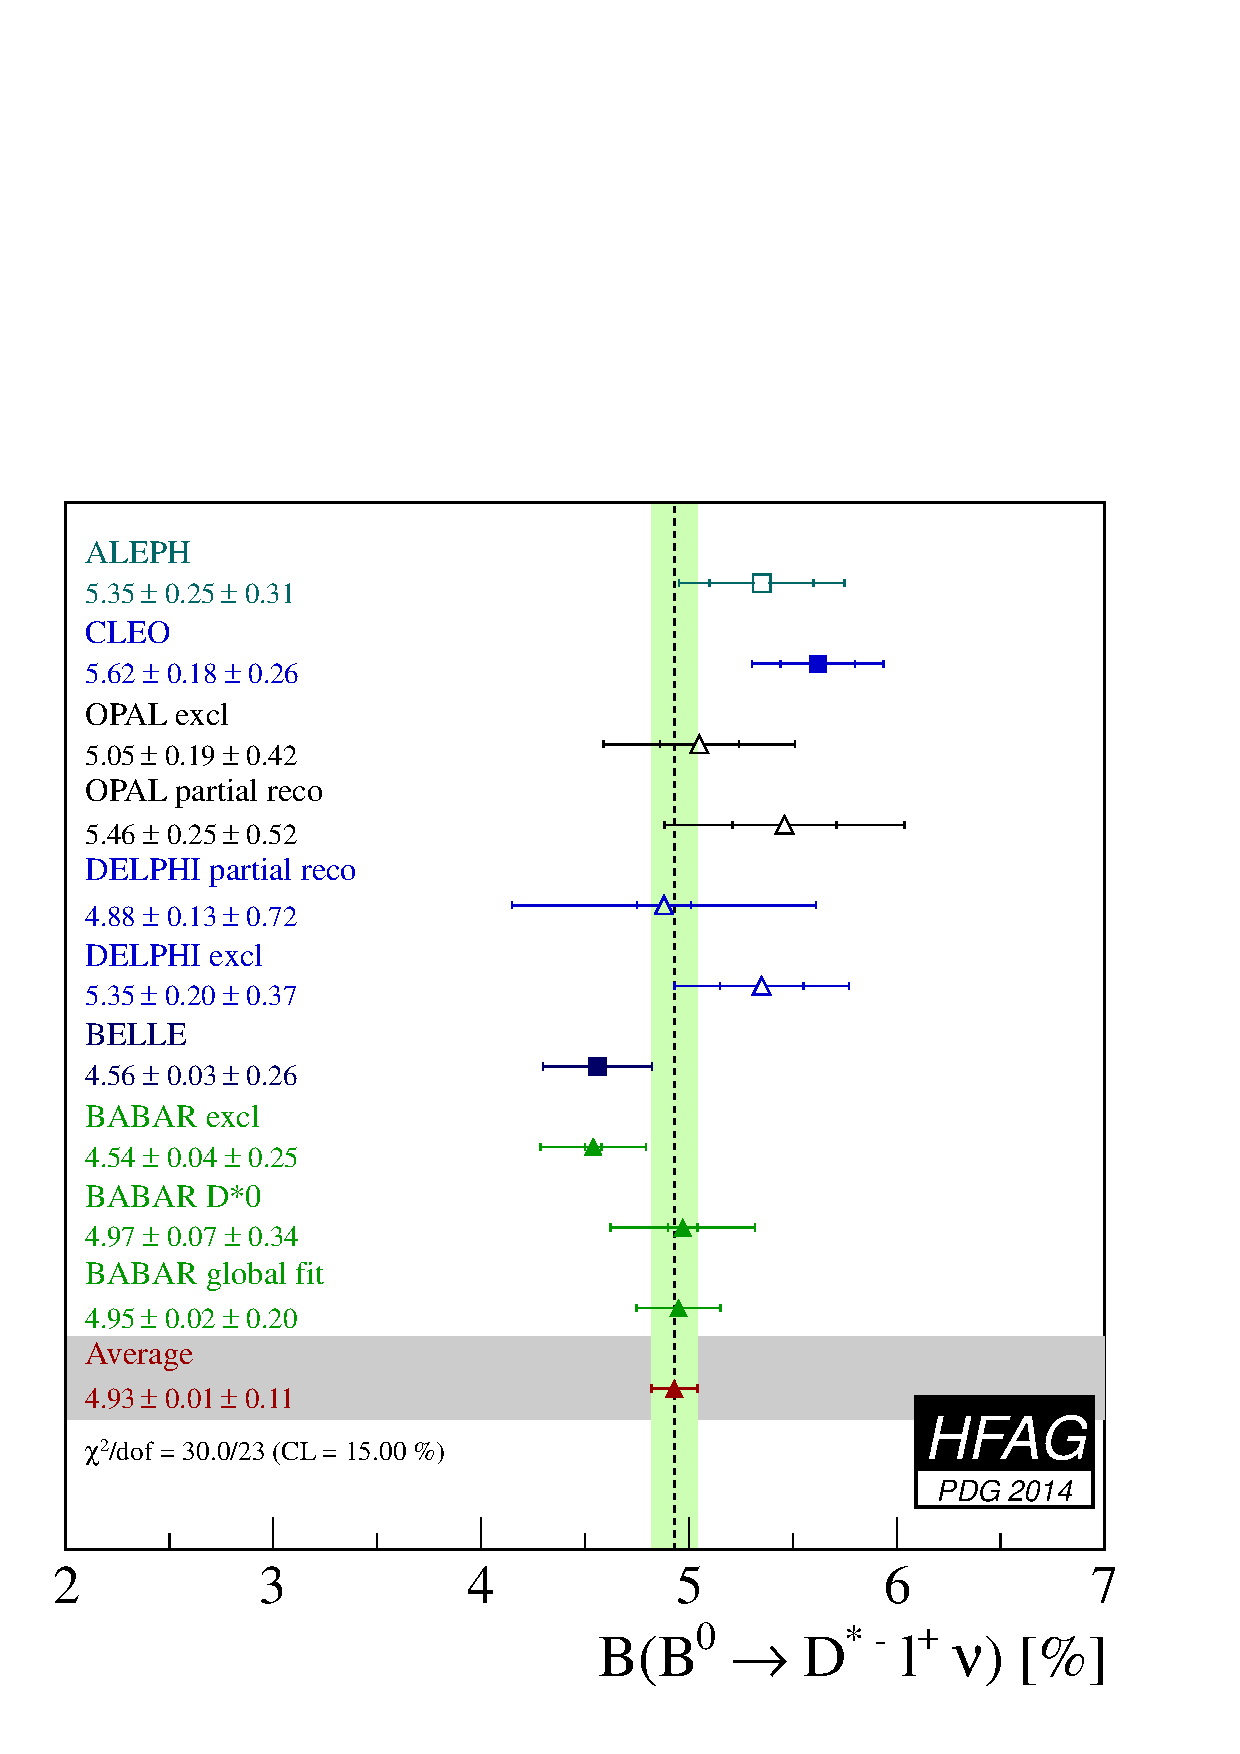
\includegraphics[width=7.5cm]{figures/slb/br_dsl_iso.pdf}
    }
    \put(  8.0, 0.0){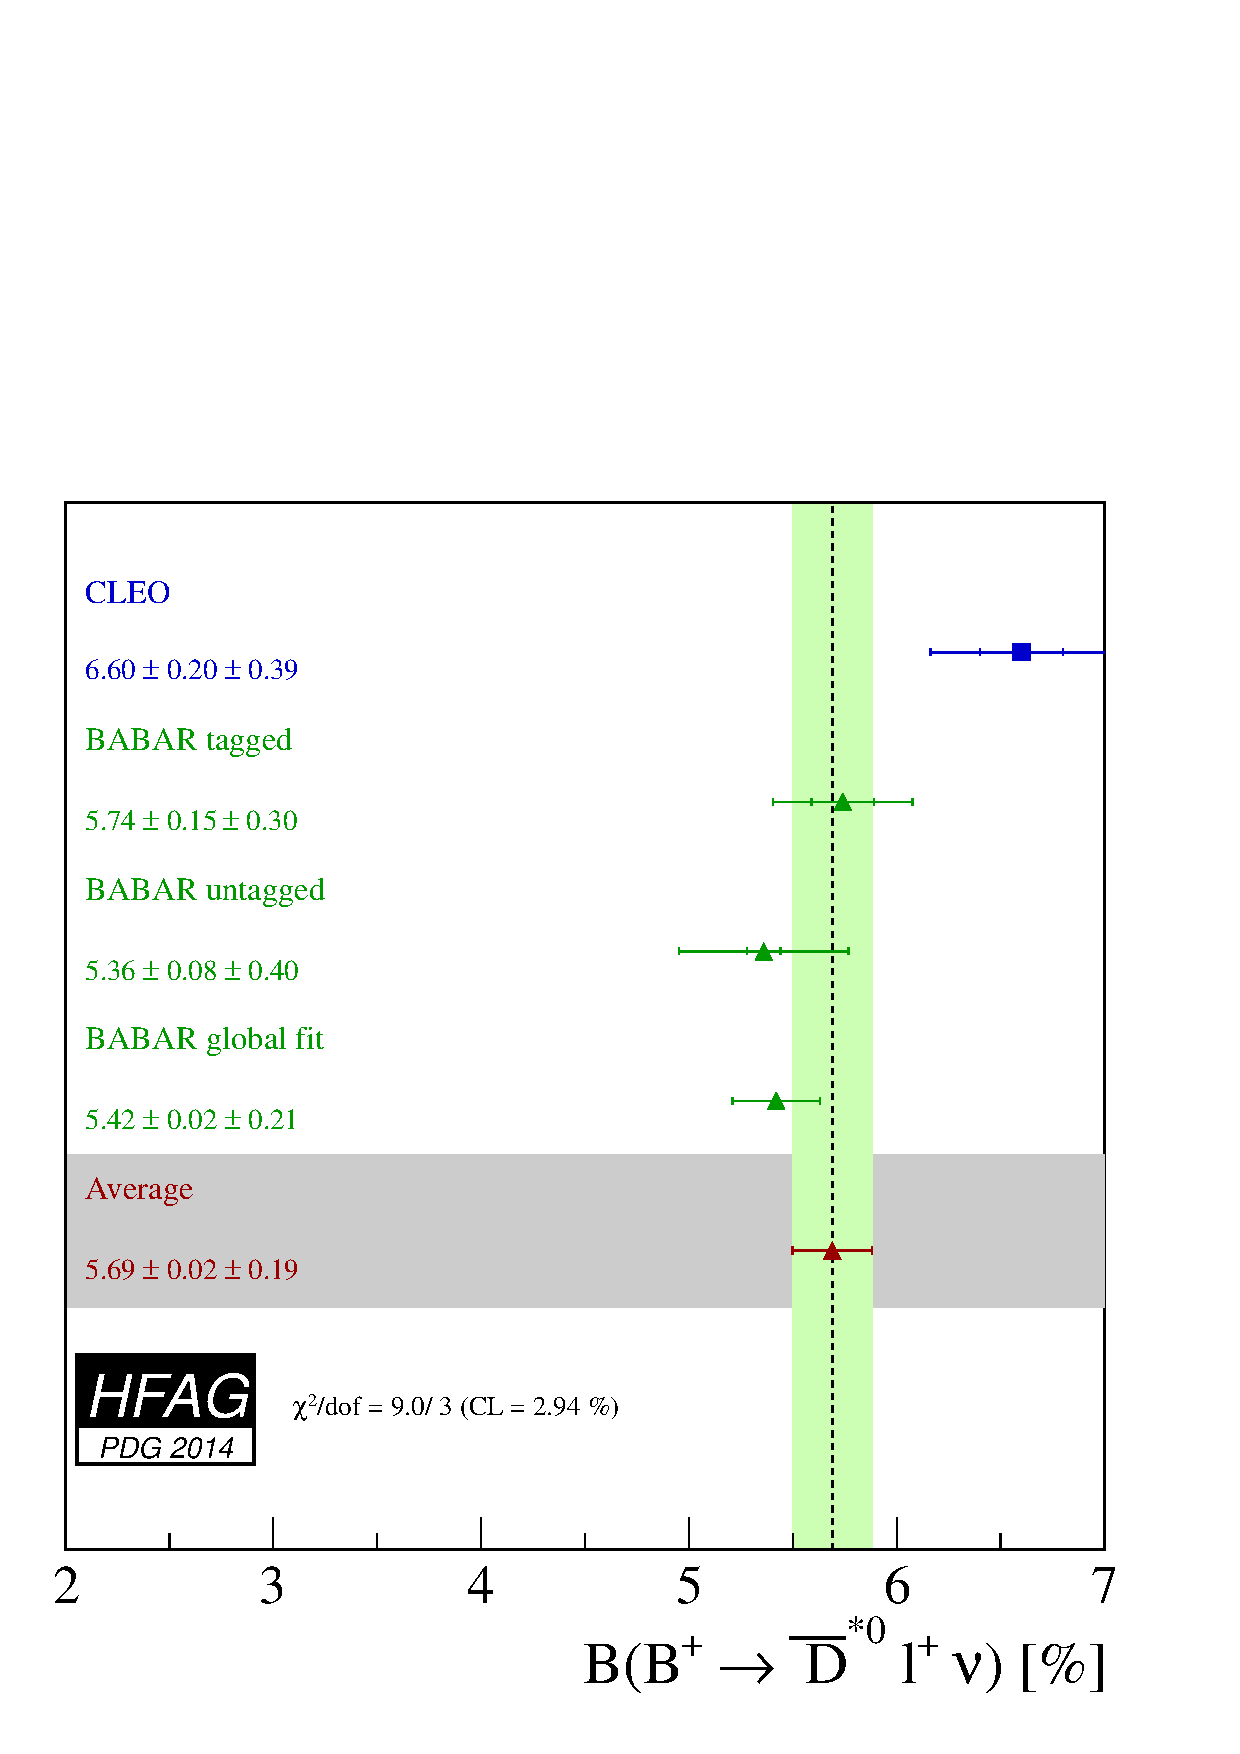
\includegraphics[width=7.5cm]{figures/slb/br_ds0l.pdf}
    }
    \put(  5.5, 6.8){{\large\bf a)}}
    \put( 14.0, 6.8){{\large\bf b)}}
  \end{picture}
  \caption{(a) Average branching fractions of exclusive semileptonic
    $B$ decays $\bar B\to D^*\ell^-\bar\nu_\ell$: (a) $\BzbDstarlnu$
    (Table~\ref{tab:dstarlnu}) and (b) $B^-\to
    D^{*0}\ell^-\bar\nu_\ell$ (Table~\ref{tab:dstar0lnu}).} \label{fig:brdsl}
  \end{center}
\end{figure}

\mysubsubsection{$\bar B\to D\ell^-\bar\nu_\ell$}
\label{slbdecays_dlnu}

The relevant form factor for the decay $\bar B\to D\ell^-\bar\nu_\ell$
is $\eta_\mathrm{EW}{\cal G}(w)$, which in CLN~\cite{CLN} is described
by only two parameters: the normalization $\eta_\mathrm{EW}{\cal
  G}(1)\vcb$ and the slope $\rho^2$.

We use the measurements of these two form factor parameters shown in
Table~\ref{tab:vcbg1} and correct them to match the latest values of
the input parameters~\cite{HFAG_sl:inputparams}. These measurements
are sensitive to both isospin states ($\BzbDplnu$ and $B^-\to
D^0\ell^-\bar\nu_\ell$). So, isospin symmetry is assumed in the analysis.
\begin{table}[!htb]
\caption{Measurements of $\bar B\to D\ell^-\bar\nu_\ell$ in the
  parameterization of Caprini, Lellouch and Neubert
  (CLN)~\cite{CLN}. The average is the result of a 2-dimensional fit
  to the rescaled measurements of ${\cal G}(1)\vcb$ and $\rho^2$. The
  $\chi^2$~value of the combination is 0.5 for 8 degrees of freedom
  (CL=$100.0\%$). The total correlation between the average ${\cal G}(1)\vcb$
  and $\rho^2$ is 0.83.}
\begin{center}
\begin{tabular}{|l|c|c|}
  \hline
  Experiment
  & ${\cal G}(1)\vcb$ [10$^{-3}$] (rescaled)
  & $\rho^2$ (rescaled)\\
  & ${\cal G}(1)\vcb$ [10$^{-3}$] (published)
  & $\rho^2$ (published)\\
  \hline \hline
  ALEPH~\hfill\cite{Buskulic:1996yq}
  & $38.89\pm 11.80_{\rm stat}\pm 6.09_{\rm syst}$
  & $0.951\pm 0.980_{\rm stat}\pm 0.357_{\rm syst}$\\
  & $31.1\pm 9.9_{\rm stat}\pm 8.6_{\rm syst}$
  & $0.70\pm 0.98_{\rm stat}\pm 0.50_{\rm syst}$\\
  \hline
  CLEO~\hfill\cite{Bartelt:1998dq}
  & $44.90\pm 5.97_{\rm stat}\pm 3.30_{\rm syst}$
  & $1.270\pm 0.250_{\rm stat}\pm 0.140_{\rm syst}$\\
  & $44.8\pm 6.1_{\rm stat}\pm 3.7_{\rm syst}$
  & $1.30\pm 0.27_{\rm stat}\pm 0.14_{\rm syst}$\\
  \hline
  \belle~\hfill\cite{Abe:2001yf}
  & $40.84\pm 4.37_{\rm stat}\pm 5.17_{\rm syst}$
  & $1.120\pm 0.220_{\rm stat}\pm 0.140_{\rm syst}$\\
  & $41.1\pm 4.4_{\rm stat}\pm 5.1_{\rm syst}$
  & $1.12\pm 0.22_{\rm stat}\pm 0.14_{\rm syst}$\\
  \hline
  \babar global fit~\hfill\cite{Aubert:2009_1}
  & $43.42\pm 0.81_{\rm stat}\pm 2.08_{\rm syst}$
  & $1.204\pm 0.040_{\rm stat}\pm 0.057_{\rm syst}$\\
  & $43.1\pm 0.8_{\rm stat}\pm 2.3_{\rm syst}$
  & $1.20\pm 0.04_{\rm stat}\pm 0.07_{\rm syst}$\\
  \hline
  \babar tagged~\hfill\cite{Aubert:2009_2}
  & $42.45\pm 1.88_{\rm stat}\pm 1.05_{\rm syst}$
  & $1.180\pm 0.089_{\rm stat}\pm 0.051_{\rm syst}$\\
  & $42.3\pm 1.9_{\rm stat}\pm 1.0_{\rm syst}$
  & $1.20\pm 0.09_{\rm stat}\pm 0.04_{\rm syst}$\\
  \hline 
  {\bf Average }
  & \mathversion{bold}$42.64\pm 0.72_{\rm stat}\pm 1.35_{\rm syst}$
  & \mathversion{bold}$1.186\pm 0.036_{\rm stat}\pm 0.041_{\rm syst}$\\
  \hline 
\end{tabular}
\end{center}
\label{tab:vcbg1}
\end{table}


The form factor parameters are extracted by a two-dimensional fit to
the rescaled measurements of $\eta_\mathrm{EW}{\cal G}(1)\vcb$ and
$\rho^2$ taking into account correlated statistical and systematic
uncertainties. The result of the fit reads
\begin{eqnarray}
  \eta_\mathrm{EW}{\cal G}(1)\vcb & = & (42.65\pm 1.53)\times
  10^{-3}~, \label{eq:vcbg1} \\
  \rho^2 & = & 1.185 \pm 0.054~,
\end{eqnarray}
with a correlation of
\begin{equation}
  \rho_{\eta_\mathrm{EW}{\cal G}(1)\vcb,\rho^2} = 0.824~.
\end{equation}
The uncertainties and the correlation coefficient include both
statistical and systematic contributions. The $\chi^2$ of the fit is
0.5 for 8 degrees of freedom, which corresponds to a confidence
level of 100.0\%. An illustration of this fit result is given in
Fig.~\ref{fig:vcbg1}.
\begin{figure}[!ht]
  \begin{center}
  \unitlength1.0cm % coordinates in cm
  \begin{picture}(14.,8.) %ys(25.,6.)
    \put(  8.0, -0.2){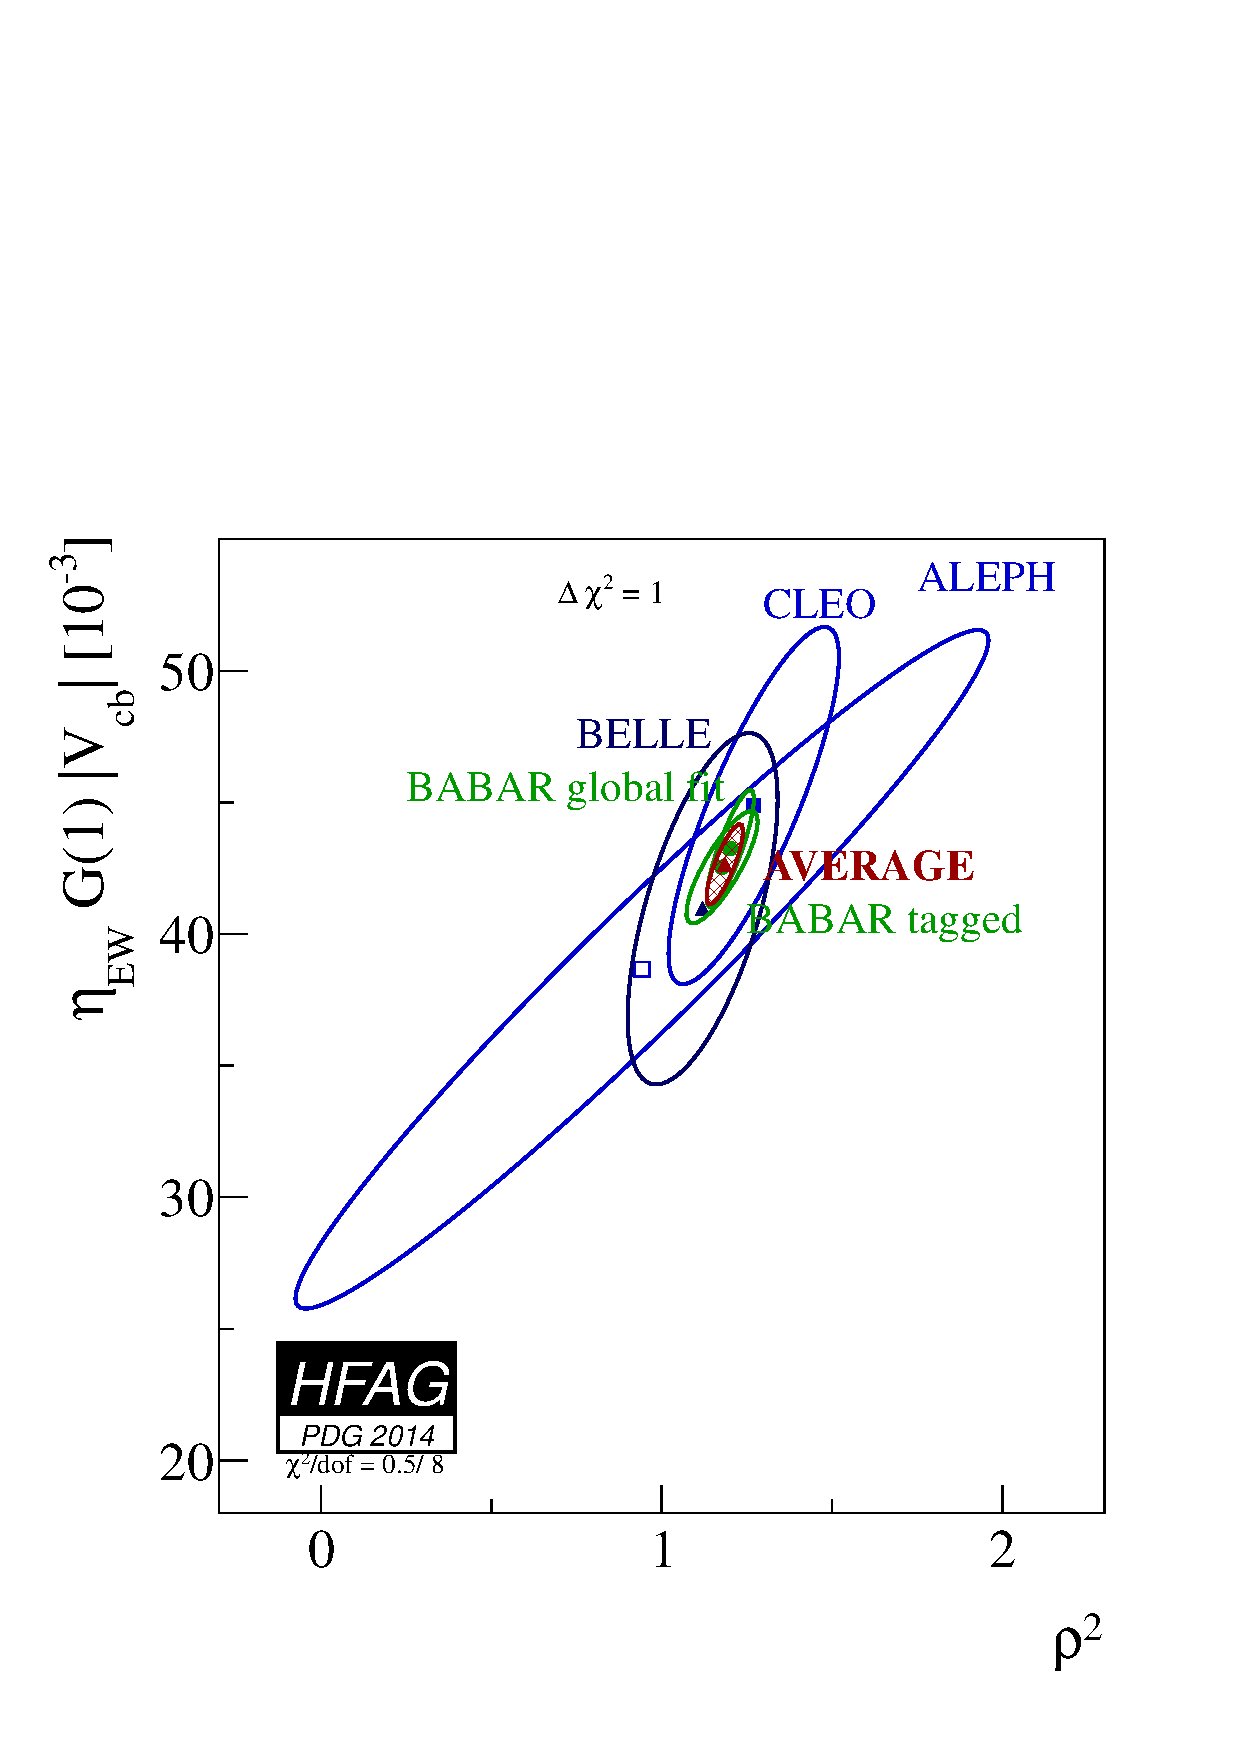
\includegraphics[width=8.0cm]{figures/slb/vcbg1_vs_rho2.pdf}
    }
    \put( -0.5,  0.0){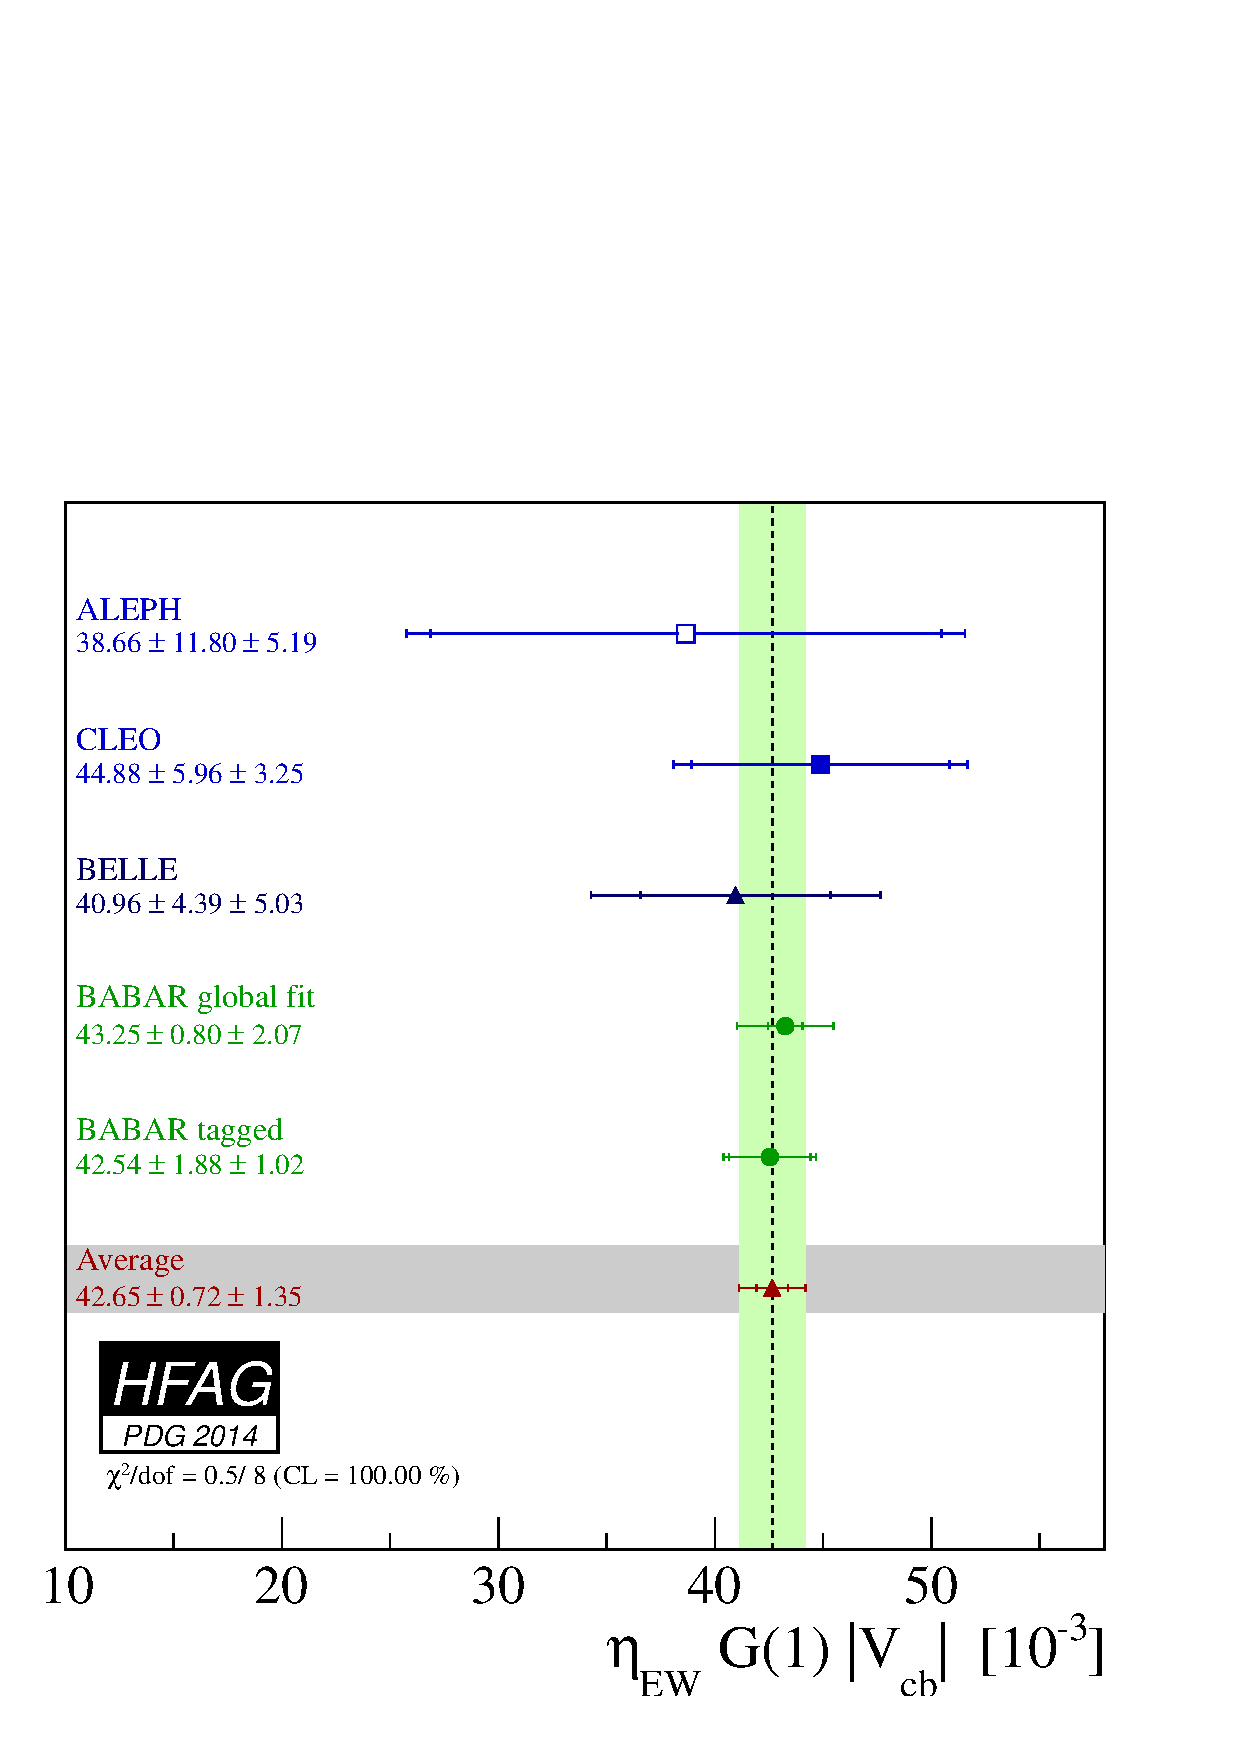
\includegraphics[width=7.5cm]{figures/slb/vcbg1.pdf}
    }
    \put(  5.5,  6.8){{\large\bf a)}}
    \put( 9.4,  6.8){{\large\bf b)}}
  \end{picture}
  \caption{(a) Illustration of the $\eta_\mathrm{EW}{\cal G}(1)\vcb$
    average. (b) Illustration of the $\eta_\mathrm{EW}{\cal G}(1)\vcb$
    vs.\ $\rho^2$ average. The error ellipses correspond  to
    $\Delta\chi^2 = 1$ (CL=39\%).}
  \label{fig:vcbg1}
  \end{center}
\end{figure}

The most recent lattice QCD result obtained for the form factor
normalization $\eta_\mathrm{EW}{\cal G}(1)$ is~\cite{Okamoto:2004xg}
\begin{equation}
  \eta_\mathrm{EW}{\cal G}(1) = 1.081\pm 0.024~,
\end{equation}
which can be used to turn Eq.~\ref{eq:vcbg1} into a determination of
$\vcb$,
\begin{equation}
  \vcb = (39.45\pm 1.42_{\rm exp}\pm 0.88_{\rm th})\times 10^{-3}~,
\end{equation}
where the first error is experimental and the second theoretical. This
number is in excellent agreement with $\vcb$ obtained from decays
$\bar B\to D^*\ell^-\bar\nu_\ell$ (Eq.~\ref{eq:vcbdstar}).

From each rescaled measurement in Table~\ref{tab:vcbg1}, we have
calculated the $\bar B\to D\ell^-\bar\nu_\ell$ form factor ${\cal
  G}(w)$ and, by numerical integration, the branching ratio of the
decay $\BzbDplnu$. The results are quoted in Table~\ref{tab:dlnuIso} and
illustrated in Fig.~\ref{fig:brdlIso}. The branching ratio found for
the average values of $\eta_\mathrm{EW}{\cal G}(1)\vcb$ and $\rho^2$ is
\begin{equation}
  \cbf(\BzbDplnu)=(2.13\pm 0.09)\%~.
\end{equation}
% ----------------------------------------------------------------------0
\begin{table}[!htb]
\caption{$\bar B^0\to D^+\ell^-\bar\nu_\ell$ branching fractions
  calculated from the rescaled measurements in Table~\ref{tab:vcbg1},
  asumming the CLN parameterization of the form factor~\cite{CLN}. The
  fit assumes isospin symmetry.}
\begin{center}
\resizebox{0.99\textwidth}{!}{
\begin{tabular}{|l|c|c|}
  \hline
  Experiment
  & $\cbf(\bar B^0\to D^+\ell^-\bar\nu_\ell)$ [\%] (calculated)
  & $\cbf(\bar B^0\to D^+\ell^-\bar\nu_\ell)$ [\%] (published)\\
  \hline \hline
  ALEPH~\hfill\cite{Buskulic:1996yq}
  & $2.16\pm 0.18_{\rm stat}\pm 0.46_{\rm syst}$
  & $2.35\pm 0.20_{\rm stat}\pm 0.44_{\rm syst}$\\
  CLEO~\hfill\cite{Bartelt:1998dq}
  & $2.19\pm 0.16_{\rm stat}\pm 0.35_{\rm syst}$
  & $2.20\pm 0.16_{\rm stat}\pm 0.19_{\rm syst}$\\
  \belle~\hfill\cite{Abe:2001yf}
  & $2.07\pm 0.12_{\rm stat}\pm 0.52_{\rm syst}$
  & $2.13\pm 0.12_{\rm stat}\pm 0.39_{\rm syst}$\\
  \babar global fit~\hfill\cite{Aubert:2009_1}
  & $2.18\pm 0.03_{\rm stat}\pm 0.13_{\rm syst}$
  & $2.34\pm 0.03_{\rm stat}\pm 0.13_{\rm syst}$\\
  \babar tagged~\hfill\cite{Aubert:2009_2}
  & $2.12\pm 0.10_{\rm stat}\pm 0.06_{\rm syst}$
  & $2.23\pm 0.11_{\rm stat}\pm 0.11_{\rm syst}$\\
  \hline 
  {\bf Average}
  & \mathversion{bold}$2.13\pm 0.03_{\rm stat}\pm 0.09_{\rm syst}$
  & \mathversion{bold}$\chi^2/\dof = 0.5/8$ (CL=$100.0\%$)\\
  \hline 
\end{tabular}
}
\end{center}
\label{tab:dlnuIso}
\end{table}
% ----------------------------------------------------------------------

\begin{figure}[!ht]
  \begin{center}
    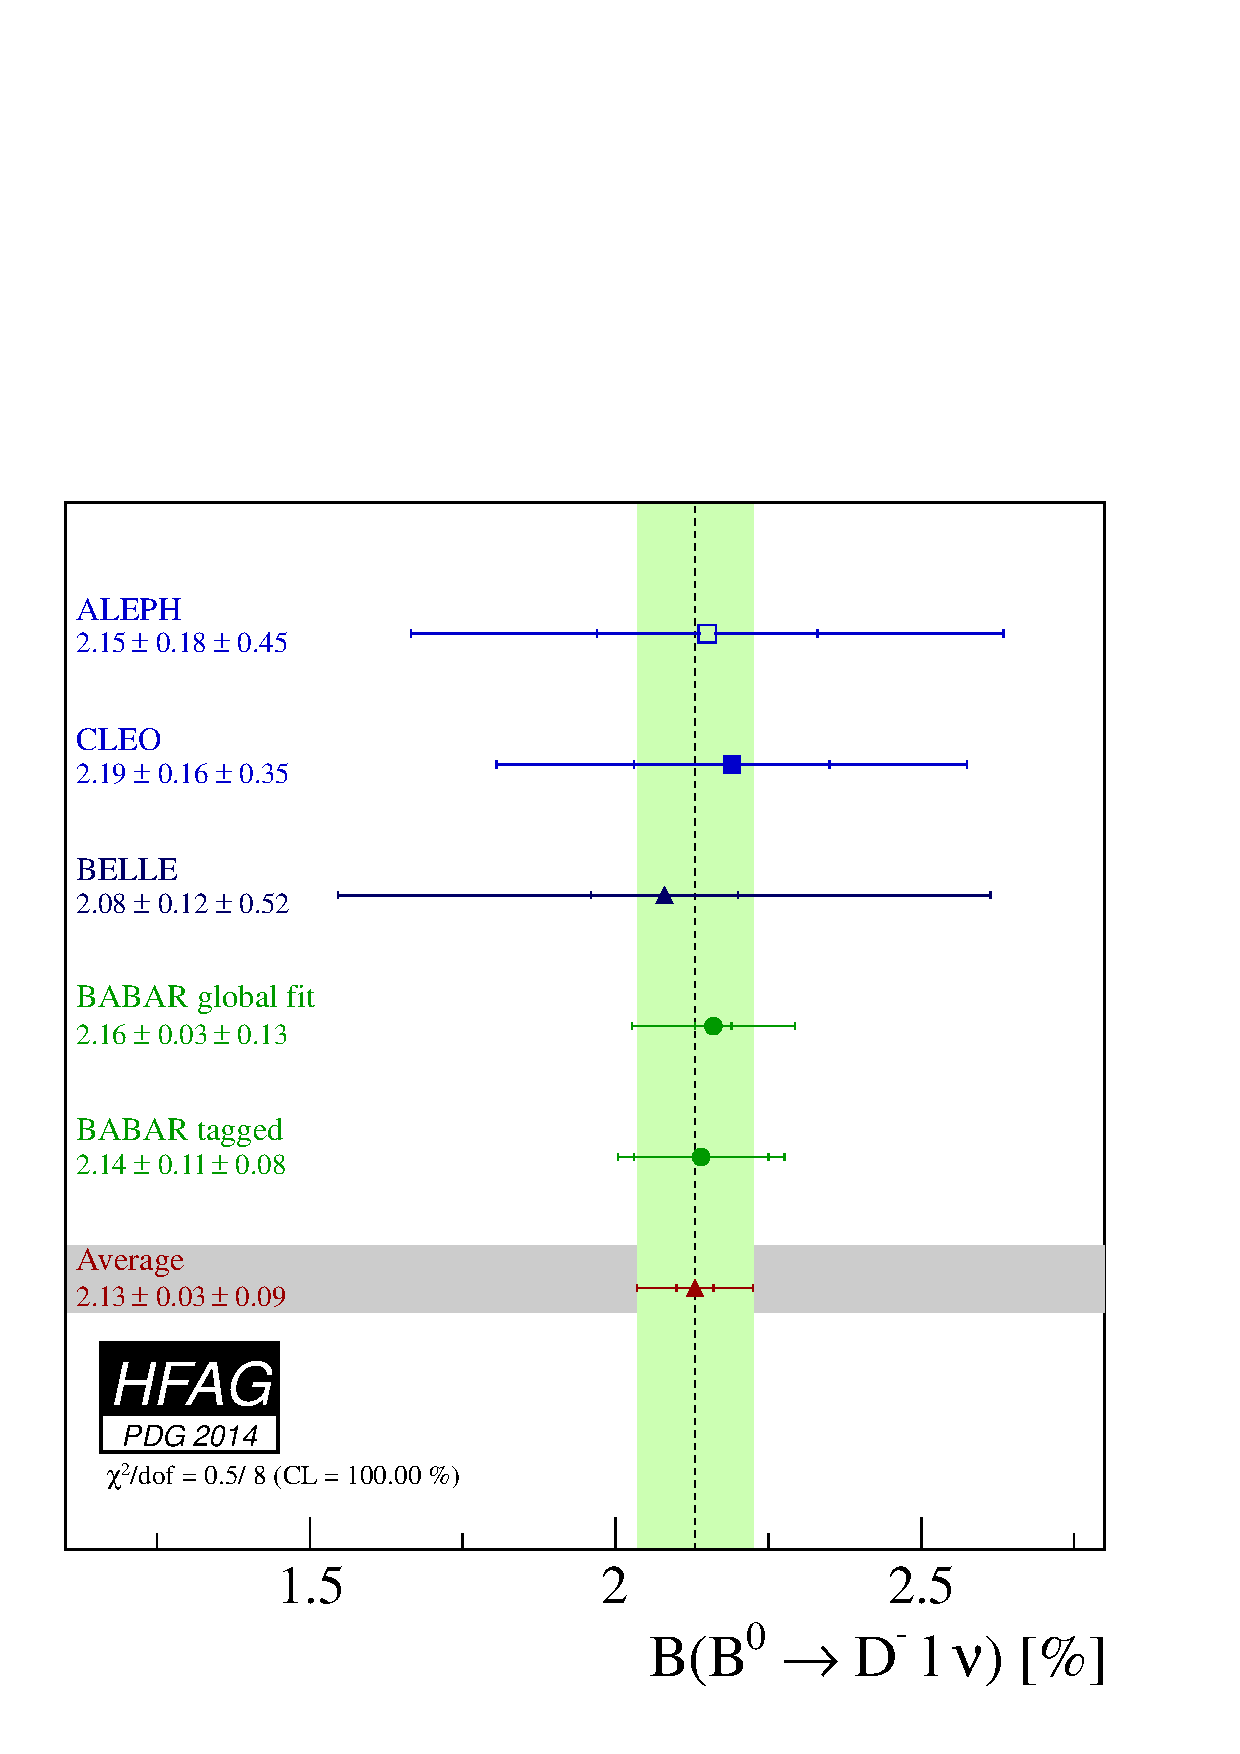
\includegraphics[width=7.55cm]{figures/slb/br_dl_iso.pdf}
    \caption{Illustration of Table~\ref{tab:dlnuIso}.} \label{fig:brdlIso}
  \end{center}
\end{figure}

We have also performed simple 1-dimensional averages of measurements
of $\BzbDplnu$ and $B^-\to D^0\ell^-\bar\nu_\ell$. These fits are
shown Tables~\ref{tab:dlnu} and \ref{tab:d0lnu}.
% ----------------------------------------------------------------------0
\begin{table}[!htb]
\caption{Average of the $\BzbDplnu$ branching fraction
  measurements. This fit uses only measurements of $\BzbDplnu$.}
\begin{center}
\begin{tabular}{|l|c|c|}
  \hline
  Experiment
  & $\cbf(\BzbDplnu)$ [\%] (rescaled)
  & $\cbf(\BzbDplnu)$ [\%] (published)\\
  \hline \hline
  ALEPH~\hfill\cite{Buskulic:1996yq}
  & $2.28\pm 0.18_{\rm stat}\pm 0.35_{\rm syst}$
  & $2.35\pm 0.20_{\rm stat}\pm 0.44_{\rm syst}$\\
  CLEO~\hfill\cite{Bartelt:1998dq}
  & $2.13\pm 0.13_{\rm stat}\pm 0.15_{\rm syst}$
  & $2.20\pm 0.16_{\rm stat}\pm 0.19_{\rm syst}$\\
  \belle~\hfill\cite{Abe:2001yf}
  & $2.11\pm 0.12_{\rm stat}\pm 0.39_{\rm syst}$
  & $2.13\pm 0.12_{\rm stat}\pm 0.39_{\rm syst}$\\
  \babar~\hfill\cite{Aubert:vcbExcl}
  & $2.22\pm 0.11_{\rm stat}\pm 0.12_{\rm syst}$
  & $2.21\pm 0.11_{\rm stat}\pm 0.12_{\rm syst}$\\
  \hline 
  {\bf Average}
  & \mathversion{bold}$2.19\pm 0.06_{\rm stat}\pm 0.10_{\rm syst}$
  & \mathversion{bold}$\chi^2/\dof = 0.2/3$ (CL=$97.3\%$)\\
  \hline 
\end{tabular}
\end{center}
\label{tab:dlnu}
\end{table}
% ----------------------------------------------------------------------

% ----------------------------------------------------------------------0
\begin{table}[!htb]
\caption{Average of the $B^-\to D^0\ell^-\bar\nu_\ell$ branching fraction
  measurements. This fit uses only measurements of $B^-\to
  D^0\ell^-\bar\nu_\ell$.}
\begin{center}
\begin{tabular}{|l|c|c|}
  \hline
  Experiment
  & $\cbf(B^-\to D^0\ell^-\bar\nu_\ell)$ [\%] (rescaled)
  & $\cbf(B^-\to D^0\ell^-\bar\nu_\ell)$ [\%] (published)\\
  \hline \hline
  CLEO~\hfill\cite{Bartelt:1998dq}
  & $2.21\pm 0.13_{\rm stat}\pm 0.17_{\rm syst}$
  & $2.32\pm 0.17_{\rm stat}\pm 0.20_{\rm syst}$\\
  \babar~\hfill\cite{Aubert:vcbExcl}
  & $2.28\pm 0.09_{\rm stat}\pm 0.09_{\rm syst}$
  & $2.33\pm 0.09_{\rm stat}\pm 0.09_{\rm syst}$\\
  \hline
  {\bf Average}
  & \mathversion{bold}$2.26\pm 0.07_{\rm stat}\pm 0.08_{\rm syst}$
  & \mathversion{bold}$\chi^2/\dof = 0.1/1$ (CL=$76.0\%$)\\
  \hline
\end{tabular}
\end{center}
\label{tab:d0lnu}
\end{table}
% ----------------------------------------------------------------------


%===================================================================
% D** 
%===================================================================

\mysubsubsection{$\bar{B} \to D^{(*)}\pi \ell^-\bar{\nu}_{\ell}$}
\label{slbdecays_dpilnu}
% --------------------

The average inclusive branching fractions for $\bar{B} \to D^{*}\pi \ell^-\bar{\nu}_{\ell}$
decays, where no constrain is applied to the hadronic $D^{(*)}\pi$ system, 
are determined by the
combination of the results provided in Table~\ref{tab:dpilnu} for 
$\bar{B}^0 \to D^0 \pi^+ \ell^-\bar{\nu}_{\ell}$, $\bar{B}^0 \to D^{*0} \pi^+
\ell^-\bar{\nu}_{\ell}$, 
$B^- \to D^+ \pi^-
\ell^-\bar{\nu}_{\ell}$, and $B^- \to D^{*+} \pi^- \ell^-\bar{\nu}_{\ell}$.
The measurements included in the average 
are scaled to a consistent set of input
parameters and their errors~\cite{HFAG_sl:inputparams}.
For both the \babar\ and Belle results, the $B$ semileptonic signal yields are
 extracted from a fit to the missing mass squared in a sample of fully
 reconstructed \BB\ events.  
Figure~\ref{fig:brdpil} illustrates the measurements and the
resulting average.

% ----------------------------------------------------------------------
\begin{table}[!htb]
\caption{Average of the branching fraction $B \to D^{(*)} \pi^- \ell^-\bar{\nu}_{\ell}$ and individual
results.}
\begin{center}
\begin{tabular}{|l|c c|}\hline
Experiment                                 &$\cbf(B^- \to D^+ \pi^- \ell^-\bar{\nu}_{\ell}) [\%]$ (rescaled) &\\
\hline
\belle  ~\hfill\cite{Live:Dss}           &$0.42 \pm0.04_{\rm stat} \pm0.05_{\rm syst}$  & \\
\babar  ~\hfill\cite{Aubert:vcbExcl}       &$0.42 \pm0.06_{\rm stat} \pm0.03_{\rm syst}$ & \\
\hline 
{\bf Average}                              &\mathversion{bold}$0.42 \pm0.05$  
   &\mathversion{bold}$\chi^2/\dof = 0.001$ (CL=$97\%$)  \\
\hline\hline

Experiment                                 &$\cbf(B^- \to D^{*+} \pi^- \ell^-\bar{\nu}_{\ell}) [\%]$ (rescaled) & \\
\hline\hline 
\belle  ~\hfill\cite{Live:Dss}           &$0.67 \pm0.08_{\rm stat} \pm0.07_{\rm syst}$  
& \\
\babar  ~\hfill\cite{Aubert:vcbExcl}       &$0.59 \pm0.05_{\rm stat} \pm0.04_{\rm syst}$  
& \\
\hline 
{\bf Average}                              &\mathversion{bold}$0.61 \pm0.05$  
 & \mathversion{bold}$\chi^2/\dof = 0.15$ (CL=$69\%$)    \\
\hline \hline

Experiment                               &$\cbf(\bar{B}^0 \to D^0 \pi^+ \ell^-\bar{\nu}_{\ell}) [\%]$ (rescaled) & \\
\hline\hline 
\belle  ~\hfill\cite{Live:Dss}           &$0.43 \pm0.07_{\rm stat} \pm0.05_{\rm syst}$ &  \\
\babar  ~\hfill\cite{Aubert:vcbExcl}     &$0.43 \pm0.08_{\rm stat} \pm0.03_{\rm syst}$ &  \\
\hline 
{\bf Average}                              &\mathversion{bold}$0.43 \pm0.06$  
   &\mathversion{bold}$\chi^2/\dof = 0.002$ (CL=$97\%$)  \\
\hline\hline

Experiment                                 &$\cbf(\bar{B}^0 \to D^{*0} \pi^+\ell^-\bar{\nu}_{\ell}) [\%]$ (rescaled) & \\
\hline\hline 
\belle  ~\hfill\cite{Live:Dss}           &$0.57 \pm0.21_{\rm stat} \pm0.07_{\rm syst}$  & \\
\babar  ~\hfill\cite{Aubert:vcbExcl}       &$0.48 \pm0.08_{\rm stat} \pm0.04_{\rm syst}$ & \\ 
\hline 
{\bf Average}                              &\mathversion{bold}$0.49 \pm0.08$  
   &\mathversion{bold}$\chi^2/\dof = 0.15$ (CL=$69\%$)  \\
\hline\hline

\end{tabular}
\end{center}
\label{tab:dpilnu}
\end{table}
% ----------------------------------------------------------------------



\begin{figure}[!ht]
 \begin{center}
  \unitlength1.0cm % coordinates in cm
  \begin{picture}(14.,8.0)  %ys(25.,6.0)
   \put( -0.5,  0.0){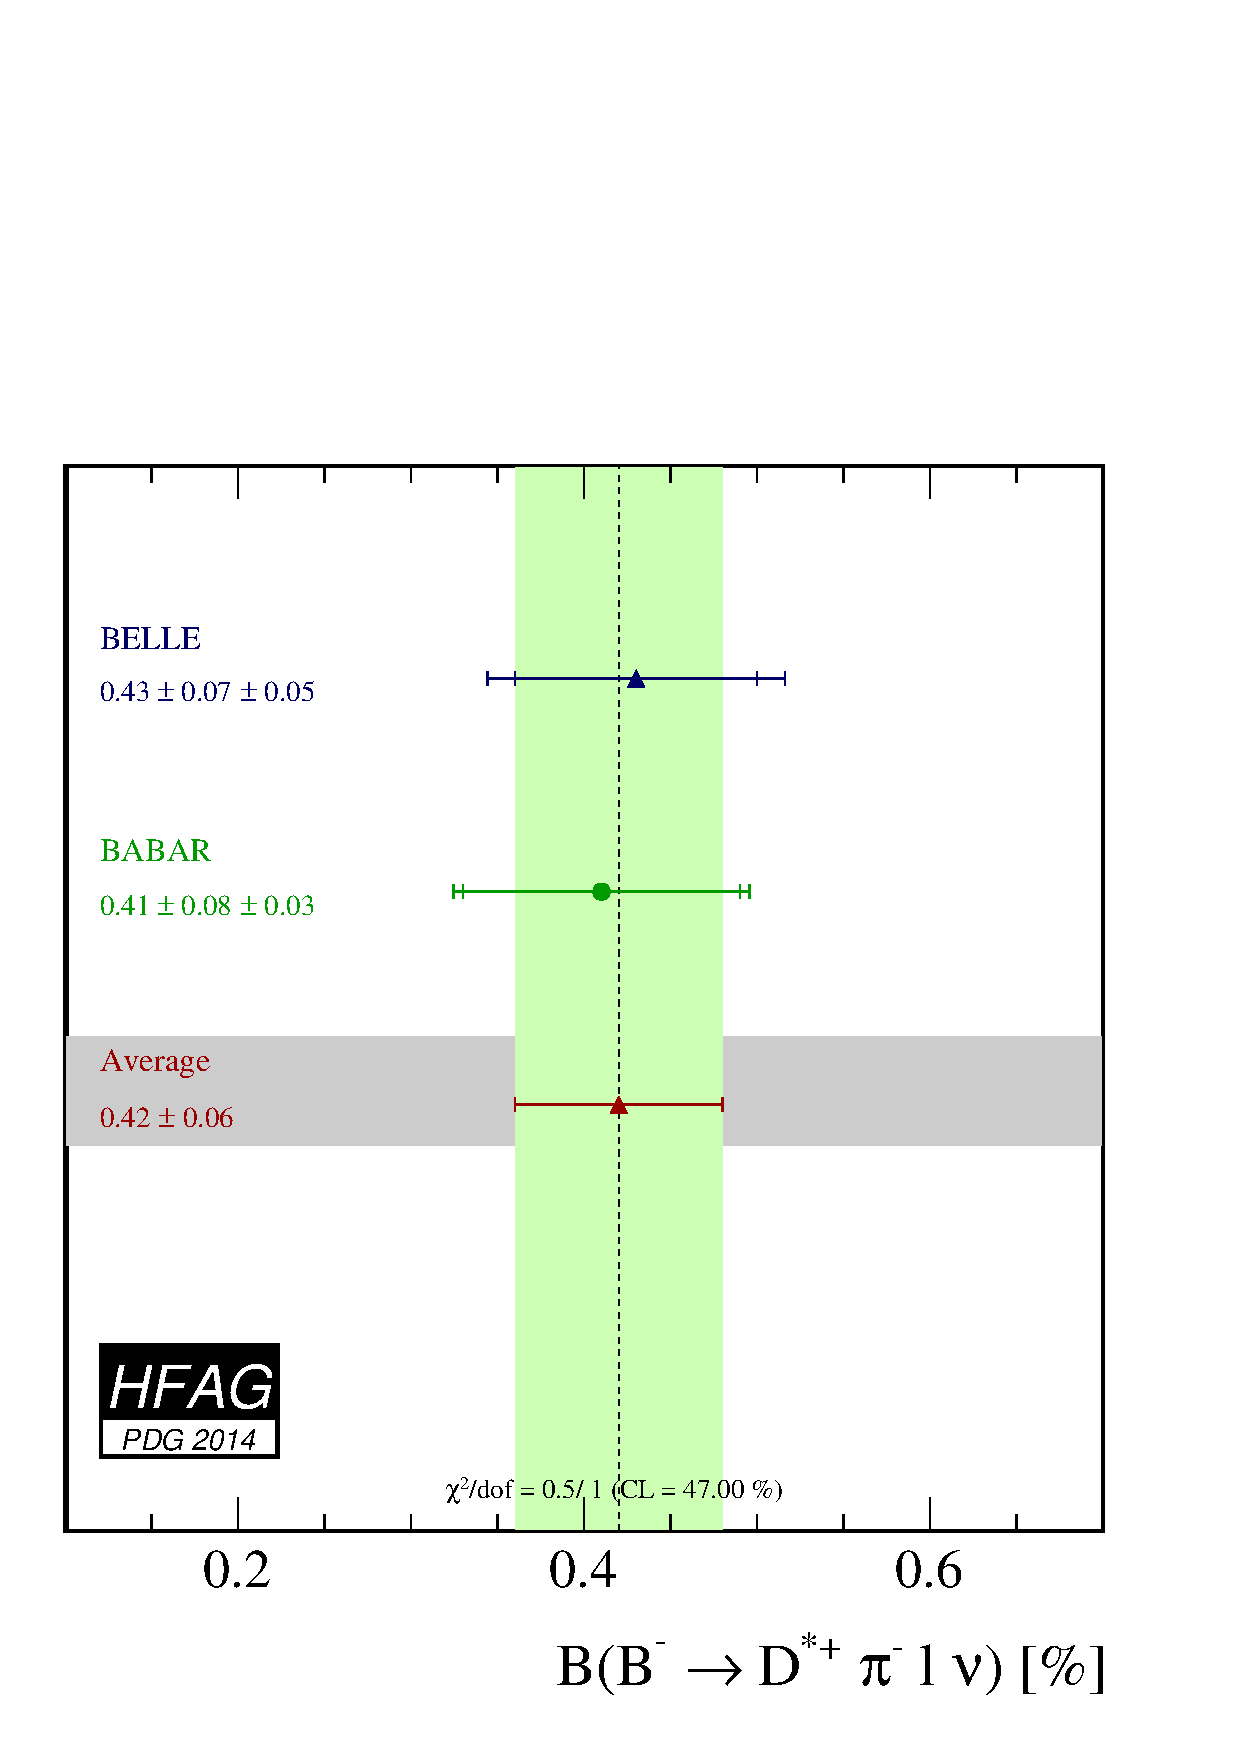
\includegraphics[width=7.55cm]{figures/slb/br_dssIncl-3.pdf}
   }
   \put(  8.0,  0.0){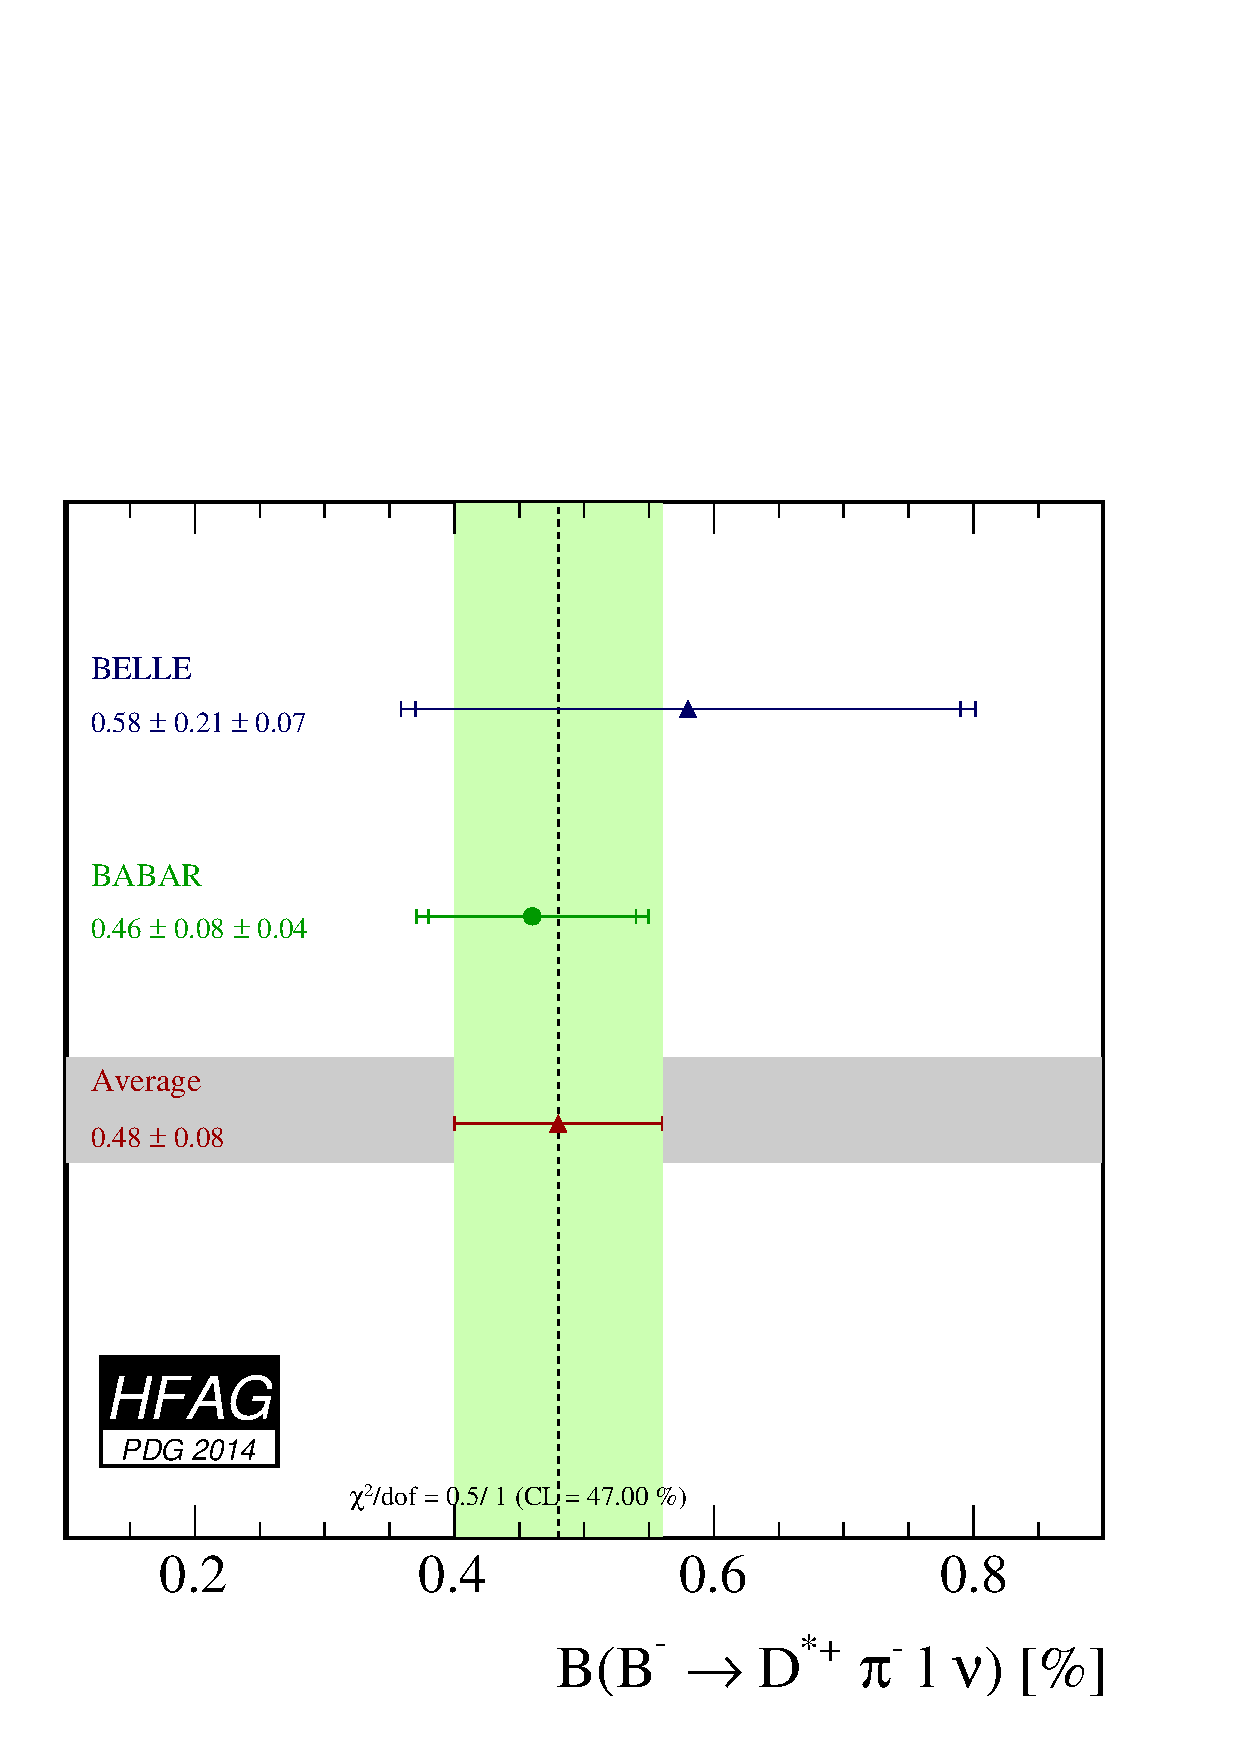
\includegraphics[width=7.8cm]{figures/slb/br_dssIncl-4.pdf}
   }
   \put(  5.5,  6.8){{\large\bf a)}}
   \put( 14.0,  6.8){{\large\bf b)}}
  \end{picture}
  \begin{picture}(14.,8.0)  %ys(25.,6.0)
   \put( -0.5,  0.0){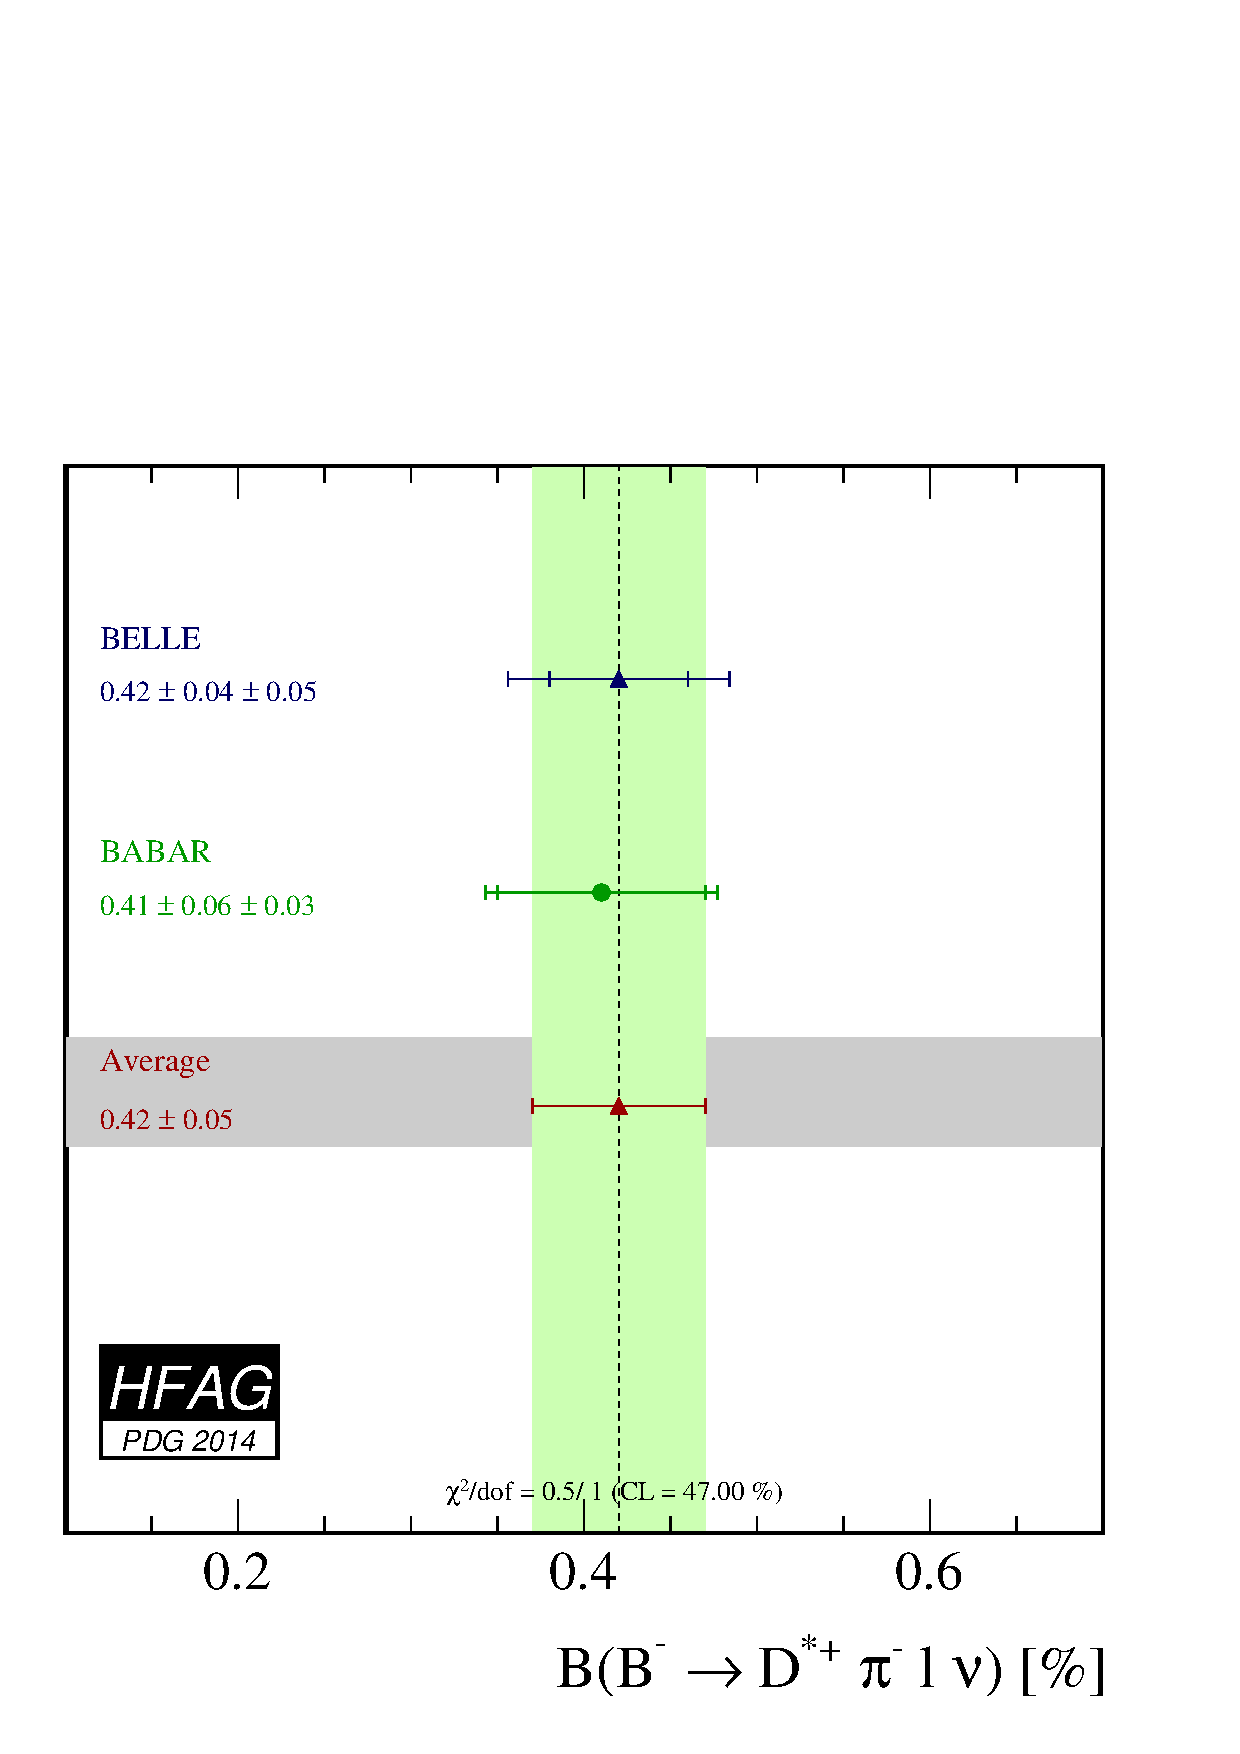
\includegraphics[width=7.55cm]{figures/slb/br_dssIncl-1.pdf}
   }
   \put(  8.0,  0.0){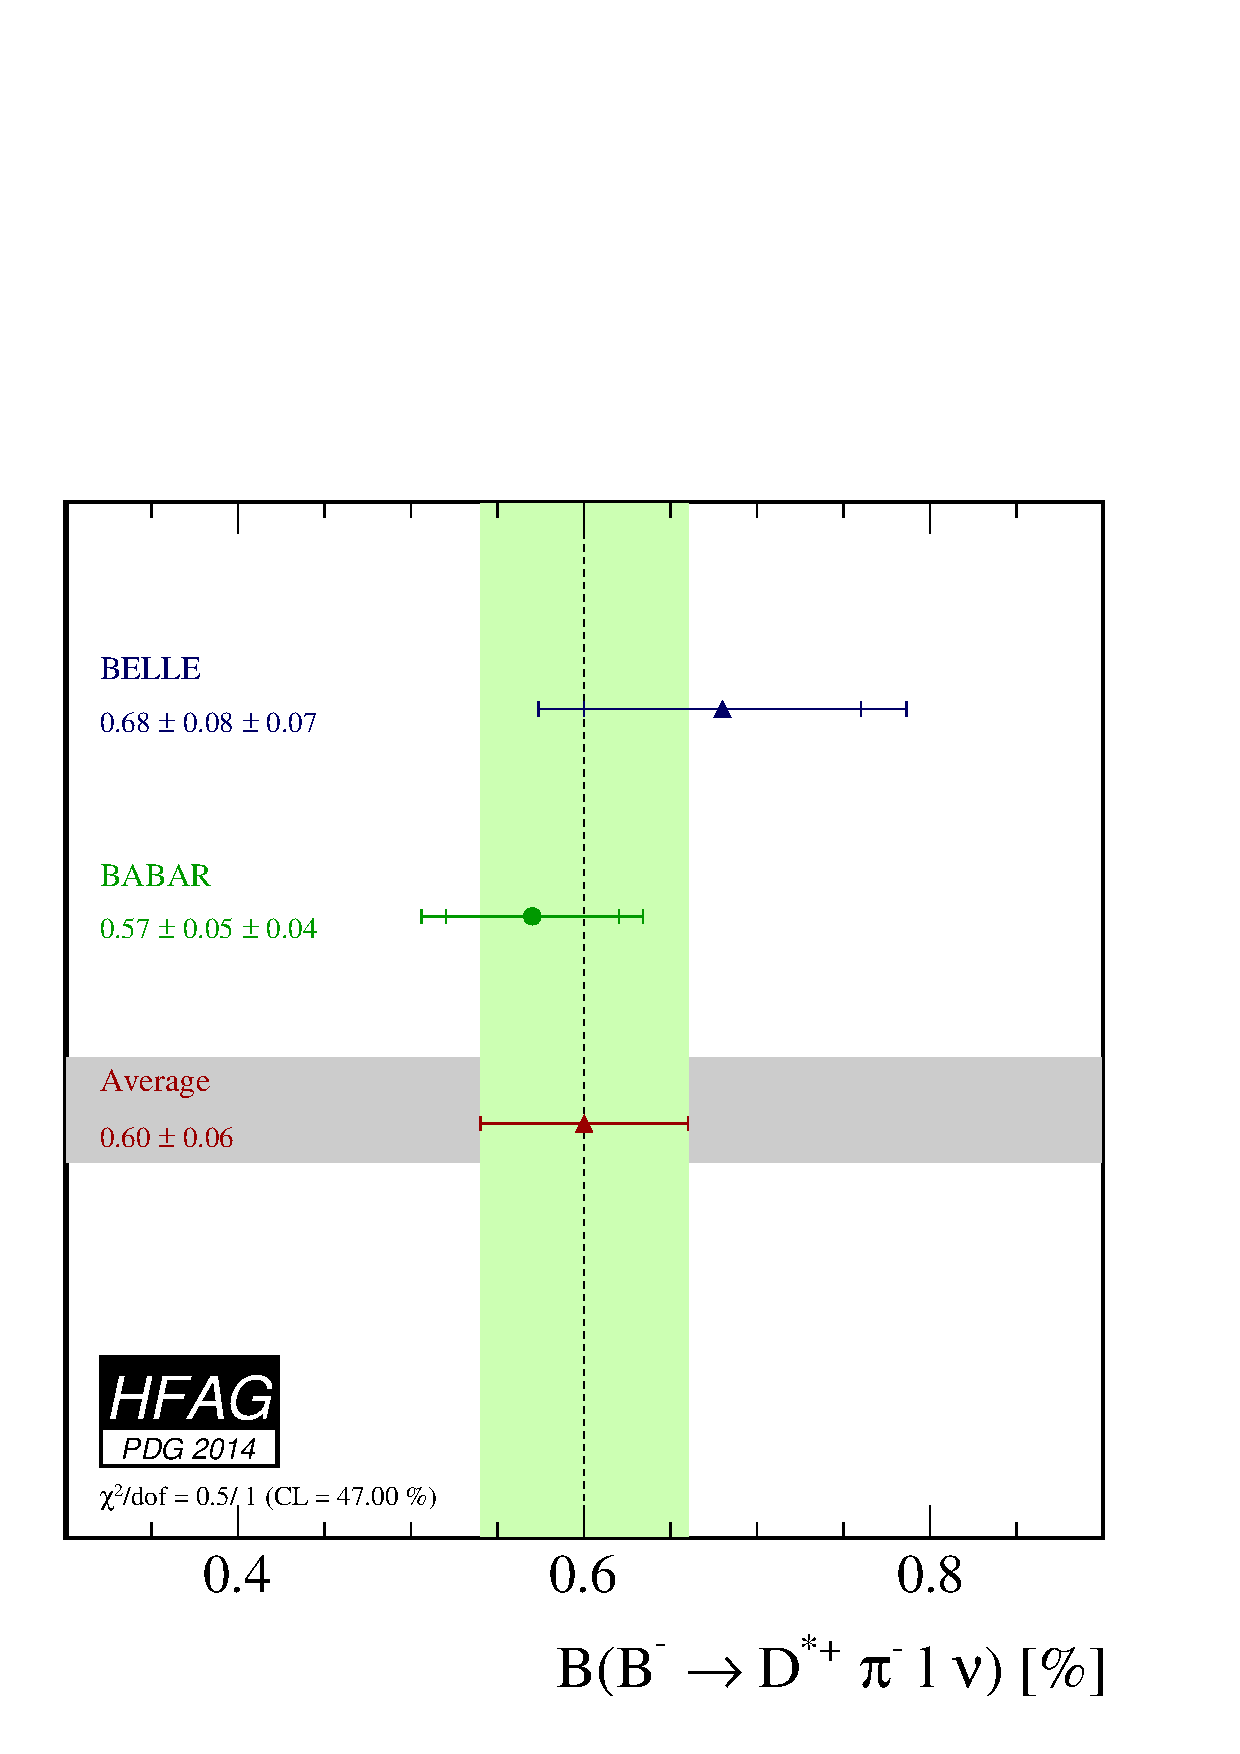
\includegraphics[width=7.8cm]{figures/slb/br_dssIncl-2.pdf}
   }
   \put(  5.5,  6.8){{\large\bf c)}}
   \put( 14.0,  6.8){{\large\bf d)}}
  \end{picture}
  \caption{Average branching fraction  of exclusive semileptonic $B$ decays
(a) $\bar{B}^0 \to D^0 \pi^+ \ell^-\bar{\nu}_{\ell}$, (b) $\bar{B}^0 \to D^{*0} \pi^+
\ell^-\bar{\nu}_{\ell}$, (c) $B^- \to D^+ \pi^-
\ell^-\bar{\nu}_{\ell}$, and (d) $B^- \to D^{*+} \pi^- \ell^-\bar{\nu}_{\ell}$.
The corresponding individual
  results are also shown.}
  \label{fig:brdpil}
 \end{center}
\end{figure}

\mysubsubsection{$\bar{B} \to D^{**} \ell^-\bar{\nu}_{\ell}$}
\label{slbdecays_dsslnu}
% -------------------

The $D^{**}$ mesons contain one charm quark and one light quark with relative angular momentum $L=1$. According to Heavy Quark Symmetry (HQS)~\cite{Isgur:1991wq}, they form one doublet of states with angular momentum $j \equiv s_q + L= 3/2$  $\left[D_1(2420), D_2^*(2460)\right]$ and another doublet with $j=1/2$ $\left[D^*_0(2400), D_1'(2430)\right]$, where $s_q$ is the light quark spin. Parity and angular momentum conservation constrain the decays allowed for each state. The $D_1$ and $D_2^*$ states decay through a D-wave to $D^*\pi$ and $D^{(*)}\pi$, respectively, and have small decay widths, while the $D_0^*$ and $D_1'$  states decay through an S-wave to $D\pi$ and $D^*\pi$ and are very broad.
For the narrow states, the average  are determined by the
combination of the results provided in Table~\ref{tab:dss1lnu} and \ref{tab:dss2lnu} for 
$\cbf(B^- \to D_1^0(D^{*+}\pi^-)\ell^-\bar{\nu}_{\ell})
\times \cbf(D_1^0 \to D^{*+}\pi^-)$ and $\cbf(B^- \to D_2^0(D^{*+}\pi^-)\ell^-\bar{\nu}_{\ell})
\times \cbf(D_2^0 \to D^{*+}\pi^-)$. 
For the broad states, the average are determined by the
combination of the results provided in Table~\ref{tab:dss1plnu} and \ref{tab:dss0lnu} for 
$\cbf(B^- \to D_1'^0(D^{*+}\pi^-)\ell^-\bar{\nu}_{\ell})
\times \cbf(D_1'^0 \to D^{*+}\pi^-)$ and $\cbf(B^- \to D_0^{*0}(D^{+}\pi^-)\ell^-\bar{\nu}_{\ell})
\times \cbf(D_0^{*0} \to D^{+}\pi^-)$. 
The measurements included in the average are scaled to a consistent set of input
parameters and their errors~\cite{HFAG_sl:inputparams}.  

For both the B-factory and the LEP and Tevatron results, the $B$ semileptonic 
signal yields are extracted from a fit to the invariant mass distribution of the $D^{(*)+}\pi^-$ system.
 Apart for the CLEO, \belle and \babar results, the other measurements 
 are for the $\bar{B} \to D^{**}(D^*\pi^-)X \ell^- \bar{\nu}_{\ell}$ final state and 
 we assume that no particles are left in the X system. The \babar tagged measurement \cite{Aubert:2009_4} measures 
 $\bar{B} \to D_2^*(D\pi)X \ell^- \bar{\nu}_{\ell}$ and it has been translated in 
 a result on  $D_2^*\to D^*\pi$ decay mode, assuming 
 ${\cal B}(D_2^*\to D\pi)/{\cal B}(D_2^*\to D^*\pi)=1.54\pm 0.15$ \cite{PDG_2014}. 
Figure~\ref{fig:brdssl} and ~\ref{fig:brdssl2} illustrate the measurements and the
resulting average.

% ----------------------------------------------------------------------0
\begin{table}[!htb]
\caption{Average of the branching fraction $\cbf(B^- \to D_1^0\ell^-\bar{\nu}_{\ell})
\times \cbf(D_1^0 \to D^{*+}\pi^-)$ and individual results. The ALEPH, OPAL and D0 measurements are for the 
$D_1(D^*\pi)X$ final state and we assum that no particles are left in the X system.}
\begin{center}
\resizebox{0.99\textwidth}{!}{
\begin{tabular}{|l|c|c|}\hline
Experiment                                 &$\cbf(B^- \to D_1^0(D^{*+}\pi^-)\ell^-\bar{\nu}_{\ell})
 [\%]$  &$\cbf(B^- \to D_1^0(D^{*+}\pi^-)\ell^-\bar{\nu}_{\ell})
 [\%]$  \\
                                                & (rescaled) & (published) \\

\hline\hline 
ALEPH ~\cite{Aleph:Dss}        &$0.440 \pm0.098_{\rm stat} \pm0.068_{\rm syst}$ 
 &$0.47 \pm0.10_{\rm stat} \pm0.07_{\rm syst}$ \\
OPAL  ~\cite{opal:Dss}         &$0.578 \pm0.210_{\rm stat} \pm0.101_{\rm syst}$  
&$0.70 \pm0.21_{\rm stat} \pm0.10_{\rm syst}$ \\
CLEO  ~\cite{cleo:Dss}         &$0.354 \pm0.085_{\rm stat} \pm0.056_{\rm syst}$ 
 &$0.373 \pm0.085_{\rm stat} \pm0.057_{\rm syst}$ \\
D0  ~\cite{D0:Dss}         &$0.215 \pm0.018_{\rm stat} \pm0.035_{\rm syst}$  
&$0.219 \pm0.018_{\rm stat} \pm0.035_{\rm syst}$ \\
\belle Tagged $B^-$ ~\cite{Live:Dss}           &$0.443 \pm0.070_{\rm stat} \pm0.059_{\rm syst}$  
&$0.42 \pm0.07_{\rm stat} \pm0.07_{\rm syst}$ \\
\belle Tagged $B^0$ ~\cite{Live:Dss}           &$0.612 \pm0.200_{\rm stat} \pm0.077_{\rm syst}$  
&$0.42 \pm0.07_{\rm stat} \pm0.07_{\rm syst}$ \\ 
\babar Tagged ~\cite{Aubert:2009_4}           &$0.278 \pm0.030_{\rm stat} \pm0.028_{\rm syst}$
&$0.29 \pm0.03_{\rm stat} \pm0.03_{\rm syst}$ \\
\babar Untagged $B^-$ ~\cite{Aubert:2008zc}           &$0.295 \pm0.017_{\rm stat} \pm0.016_{\rm syst}$
&$0.30 \pm0.02_{\rm stat} \pm0.02_{\rm syst}$ \\
\babar Untagged $B^0$ ~\cite{Aubert:2008zc}           &$0.299 \pm0.026_{\rm stat} \pm0.027_{\rm syst}$
&$0.30 \pm0.02_{\rm stat} \pm0.02_{\rm syst}$ \\
\hline
{\bf Average}                              &\mathversion{bold}$0.285 \pm0.011 \pm 0.014$ 
    &\mathversion{bold}$\chi^2/\dof = 13.0/8$ (CL=$11.1\%$)  \\
\hline 
\end{tabular}
}
\end{center}
\label{tab:dss1lnu}
\end{table}
% ----------------------------------------------------------------------


% ----------------------------------------------------------------------0
\begin{table}[!htb]
\caption{Average of the branching fraction $\cbf(B^- \to D_2^0(D^{*+}\pi^-)\ell^-\bar{\nu}_{\ell})
\times \cbf(D_2^0 \to D^{*+}\pi^-))$ and individual results. The D0 measurement is for the $D_2^*(D^*\pi)X$
final state and we assume that no particles are left in the X system.
The \babar tagged measurement
has been translated in a result on $D_2^*\to D^*\pi$ decay mode, assuming 
${\cal B}(D_2^*\to D\pi)/{\cal B}(D_2^*\to D^*\pi)=1.54\pm 0.15$, \cite{PDG_2014}.}
\begin{center}
\resizebox{0.99\textwidth}{!}{
\begin{tabular}{|l|c|c|}\hline
Experiment                                 &$\cbf(B^- \to D_2^0(D^{*+}\pi^-)\ell^-\bar{\nu}_{\ell})
) [\%]$  &$\cbf(B^- \to D_2^0(D^{*+}\pi^-)\ell^-\bar{\nu}_{\ell})
) [\%]$  \\
                                                & (rescaled) & (published) \\
\hline\hline 
CLEO  ~\cite{cleo:Dss}         &$0.056 \pm0.066_{\rm stat} \pm0.011_{\rm syst}$ 
 &$0.059 \pm0.066_{\rm stat} \pm0.011_{\rm syst}$ \\
D0  ~\cite{D0:Dss}         &$0.087 \pm0.018_{\rm stat} \pm0.020_{\rm syst}$  
&$0.088 \pm0.018_{\rm stat} \pm0.020_{\rm syst}$ \\
\belle  ~\cite{Live:Dss}           &$0.190 \pm0.060_{\rm stat} \pm0.025_{\rm syst}$  
&$0.18 \pm0.06_{\rm stat} \pm0.03_{\rm syst}$ \\
\babar tagged ~\cite{Aubert:2009_4}           &$0.076 \pm0.013_{\rm stat} \pm0.009_{\rm syst}$
&$0.078 \pm0.013_{\rm stat} \pm0.010_{\rm syst}$ \\
\babar untagged $B^-$ ~\cite{Aubert:2009_5}           &$0.090 \pm0.009_{\rm stat} \pm0.007_{\rm syst}$
&$0.087 \pm0.013_{\rm stat} \pm0.007_{\rm syst}$ \\
\babar untagged $B^0$ ~\cite{Aubert:2009_5}           &$0.067 \pm0.010_{\rm stat} \pm0.004_{\rm syst}$
&$0.087 \pm0.013_{\rm stat} \pm0.007_{\rm syst}$ \\
\hline
{\bf Average}                              &\mathversion{bold}$0.078 \pm0.007 \pm 0.004$ 
    &\mathversion{bold}$\chi^2/\dof = 5.6/5$ (CL=$34.7\%$)  \\
\hline 
\end{tabular}
}
\end{center}
\label{tab:dss2lnu}
\end{table}
% ----------------------------------------------------------------------


% ----------------------------------------------------------------------
\begin{table}[!htb]
\caption{Average of the branching fraction $\cbf(B^- \to D_1^{'0}(D^{*+}\pi^-)\ell^-\bar{\nu}_{\ell})
\times \cbf(D_1^{'0} \to D^{*+}\pi^-))$ and individual results. The DELPHI measurement 
is for the final state $D_1'(D^*\pi)X$ and we assume that no particles are left in the X system.}
\begin{center}
\begin{tabular}{|l|c|c|}\hline
Experiment                                 &$\cbf(B^- \to D_1^{'0}(D^{*+}\pi^-)\ell^-\bar{\nu}_{\ell})
) [\%]$  &$\cbf(B^- \to D_1^{'0}(D^{*+}\pi^-)\ell^-\bar{\nu}_{\ell})
) [\%]$  \\
                                                & (rescaled) & (published) \\
\hline\hline 
DELPHI ~\cite{Abdallah:2005cx}        &$0.74 \pm0.17_{\rm stat} \pm0.18_{\rm syst}$ 
 &$0.83 \pm0.17_{\rm stat} \pm0.18_{\rm syst}$ \\
\belle  ~\cite{Live:Dss}           &$-0.03 \pm0.06_{\rm stat} \pm0.07_{\rm syst}$  
&$-0.03 \pm0.06_{\rm stat} \pm0.07_{\rm syst}$ \\
\babar  ~\cite{Aubert:2009_4}           &$0.26 \pm0.04_{\rm stat} \pm0.04_{\rm syst}$
&$0.27 \pm0.04_{\rm stat} \pm0.05_{\rm syst}$ \\
\hline
{\bf Average}                              &\mathversion{bold}$0.13 \pm 0.03 \pm0.02$ 
    &\mathversion{bold}$\chi^2/\dof = 18./2$ (CL=$0.0001\%$)  \\
\hline 
\end{tabular}
\end{center}
\label{tab:dss1plnu}
\end{table}
% ----------------------------------------------------------------------


% ----------------------------------------------------------------------0
\begin{table}[!htb]
\caption{Average of the branching fraction $\cbf(B^- \to D_0^{*0}(D^{+}\pi^-)\ell^-\bar{\nu}_{\ell})
\times \cbf(D_0^{*0} \to D^{+}\pi^-))$ and individual
results. }
\begin{center}
\begin{tabular}{|l|c|c|}\hline
Experiment                                 &$\cbf(B^- \to D_0^{*0}(D^{+}\pi^-)\ell^-\bar{\nu}_{\ell})
) [\%]$  &$\cbf(B^- \to D_0^{*0}(D^{+}\pi^-)\ell^-\bar{\nu}_{\ell})
) [\%]$ \\
						& (rescaled) & (published) \\
\hline\hline 
\belle Tagged $B^-$ ~\hfill\cite{Live:Dss}           &$0.25 \pm0.04_{\rm stat} \pm0.06_{\rm syst}$  
&$0.24 \pm0.04_{\rm stat} \pm0.06_{\rm syst}$ \\
\belle Tagged $B^0$ ~\hfill\cite{Live:Dss}           &$0.23 \pm0.08_{\rm stat} \pm0.06_{\rm syst}$  
&$0.24 \pm0.04_{\rm stat} \pm0.06_{\rm syst}$ \\
\babar Tagged ~\hfill\cite{Aubert:2009_4}            &$0.31 \pm0.04_{\rm stat} \pm0.05_{\rm syst}$
&$0.26 \pm0.05_{\rm stat} \pm0.04_{\rm syst}$ \\
\hline
{\bf Average}                              &\mathversion{bold}$0.29 \pm 0.03 \pm0.04$ 
    &\mathversion{bold}$\chi^2/\dof = 0.61/2$ (CL=$73.6\%$)  \\
\hline 
\end{tabular}
\end{center}
\label{tab:dss0lnu}
\end{table}
% ----------------------------------------------------------------------



\begin{figure}[!ht]
 \begin{center}
  \unitlength1.0cm % coordinates in cm
  \begin{picture}(14.,8.0)  %ys(25.,6.0)
   \put( -0.5,  0.0){\includegraphics[width=7.8cm]{figures/slb/br_dss1l.pdf}
   }
   \put(  8.0,  0.0){\includegraphics[width=7.55cm]{figures/slb/br_dss2l.pdf}
   }
   \put(  5.5,  7.0){{\large\bf a)}}
   \put( 14.0,  7.0){{\large\bf b)}}
  \end{picture}
  \caption{Average of the product of branching fraction (a) 
  $\cbf(B^- \to D_1^0(D^{*+}\pi^-)\ell^-\bar{\nu}_{\ell})
\times \cbf(D_1^0 \to D^{*+}\pi^-)$ and (b) $\cbf(B^- \to D_2^0(D^{*+}\pi^-)\ell^-\bar{\nu}_{\ell})
\times \cbf(D_2^0 \to D^{*+}\pi^-)$. The corresponding individual results are also shown.}
  \label{fig:brdssl}
 \end{center}
\end{figure}

\begin{figure}[!ht]
 \begin{center}
  \unitlength1.0cm % coordinates in cm
  \begin{picture}(14.,8.0)  %ys(25.,6.0)
   \put( -0.5,  0.0){\includegraphics[width=7.8cm]{figures/slb/br_dss1primel.pdf}
   }
   \put(  8.0,  0.0){\includegraphics[width=7.8cm]{figures/slb/br_dss00l.pdf}
   }
   \put(  5.5,  7.3){{\large\bf a)}}
   \put( 14.4,  7.3){{\large\bf b)}}
  \end{picture}
  \caption{Average of the product of branching fraction (a) 
  $\cbf(B^- \to D_1'^0(D^{*+}\pi^-)\ell^-\bar{\nu}_{\ell})
\times \cbf(D_1'^0 \to D^{*+}\pi^-)$ and (b) $\cbf(B^- \to D_0^{*0}(D^{*+}\pi^-)\ell^-\bar{\nu}_{\ell})
\times \cbf(D_0^{*0} \to D^{+}\pi^-)$
The corresponding individual
  results are also shown.}
  \label{fig:brdssl2}
 \end{center}
\end{figure}


%
% ======================================================================
% Inclusive CKM-favoured decays
% -- \include{b2cincl.tex}
% ======================================================================
\subsection{Inclusive CKM-favored decays}
\label{slbdecays_b2cincl}
% -------------------------------------------

\subsubsection{Global analysis of $\bar B\to X_c\ell^-\bar\nu_\ell$}

The semileptonic width $\Gamma(\bar B\to X_c\ell^-\bar\nu_\ell)$ has
been calculated in the framework of the Operator Product
Expansion~\cite{Shifman:1986mx,*Chay:1990da,*Bigi:1992su,*Bigi:1992su_erratum}.
The result is a double-expansion in $\Lambda_{\rm QCD}/m_b$ and
$\alpha_s$, which depends on a number of non-perturbative
parameters. These parameters give information on the dynamics of the
$b$-quark inside the $B$~hadron and can be measured using other
observables in $\bar B\to X_c\ell^-\bar\nu_\ell$ decays, such as the
moments of the lepton energy and the hadronic mass spectrum.

Two independent sets of theoretical expressions, named after the
definition of the $b$-quark mass used, are available for this kind of
analysis: the kinetic~\cite{Benson:2003kp,Gambino:2004qm,Gambino:2011cq} and 1S
scheme expressions~\cite{Bauer:2004ve}. The non-perturbative
parameters in the kinetic scheme
are: the quark masses $m_b$ and $m_c$, $\mu^2_\pi$ and
$\mu^2_G$ at $O(1/m^2_b)$, and $\rho^3_D$ and $\rho^3_{LS}$ at
$O(1/m^3_b)$. In the 1S scheme, the parameters are: $m_b$, $\lambda_1$
at $O(1/m^2_b)$, and $\rho_1$, $\tau_1$, $\tau_2$ and $\tau_3$ at
$O(1/m^3_b)$. Note that due to the different definitions, the results
for the quark masses cannot be compared directly between the two
schemes.

Our analysis uses all available measurements of moments in $\bar B\to
X_c\ell^-\bar\nu_\ell$, excluding only points with too high
correlation to avoid numerical issues. The list of included
measurements is given in
Table~\ref{tab:gf_input}. The only external input is the average
lifetime~$\tau_B$ of neutral and charged $B$~mesons, taken to be
$(1.579\pm 0.005)$~ps (Sec.~\ref{sec:life_mix}).
\begin{table}[!htb]
\caption{Experimental inputs used in the global analysis of $\bar B\to
  X_c\ell^-\bar\nu_\ell$. $n$ is the order of the moment, $c$ is the
  threshold value of the lepton momentum in GeV. In total, there are
  23 measurements from \babar, 15 measurements from Belle and 12 from
  other experiments.} \label{tab:gf_input}
\begin{center}
\begin{tabular}{|l|l|l|}
  \hline
  Experiment
  & Hadron moments $\langle M^n_X\rangle$
  & Lepton moments $\langle E^n_\ell\rangle$\\
  \hline \hline
  \babar & $n=2$, $c=0.9,1.1,1.3,1.5$ & $n=0$, $c=0.6,1.2,1.5$\\
  & $n=4$, $c=0.8,1.0,1.2,1.4$ & $n=1$, $c=0.6,0.8,1.0,1.2,1.5$\\
  & $n=6$, $c=0.9,1.3$~\cite{Aubert:2009qda} & $n=2$, $c=0.6,1.0,1.5$\\
  & & $n=3$, $c=0.8,1.2$~\cite{Aubert:2009qda,Aubert:2004td}\\
  \hline
  Belle & $n=2$, $c=0.7,1.1,1.3,1.5$ & $n=0$, $c=0.6,1.4$\\
  & $n=4$, $c=0.7,0.9,1.3$~\cite{Schwanda:2006nf} & $n=1$,
  $c=1.0,1.4$\\
  & & $n=2$, $c=0.6,1.4$\\
  & & $n=3$, $c=0.8,1.2$~\cite{Urquijo:2006wd}\\
  \hline
  CDF & $n=2$, $c=0.7$ & \\
  & $n=4$, $c=0.7$~\cite{Acosta:2005qh} & \\
  \hline
  CLEO & $n=2$, $c=1.0,1.5$ & \\
  & $n=4$, $c=1.0,1.5$~\cite{Csorna:2004kp} & \\
  \hline
  DELPHI & $n=2$, $c=0.0$ & $n=1$, $c=0.0$ \\
  & $n=4$, $c=0.0$ & $n=2$, $c=0.0$ \\
  & $n=6$, $c=0.0$~\cite{Abdallah:2005cx} & $n=3$,
  $c=0.0$~\cite{Abdallah:2005cx}\\
  \hline
\end{tabular}
\end{center}
\end{table}

Both in the kinetic and 1S schemes, the moments in $\bar B\to
X_c\ell^-\bar\nu_\ell$ are not sufficient to determine the $b$-quark
mass precisely. In the kinetic scheme analysis we constrain the $c$-quark
mass (defined in the $\overline{\rm MS}$ scheme) to the value of
Ref.~\cite{Chetyrkin:2009fv},
\begin{equation}
  m_c^{\overline{\rm MS}}(3~{\rm GeV})=(0.986\pm 0.013)~{\rm GeV}~.
\end{equation}
In the 1S~scheme analysis, the $b$-quark mass is constrained with
measurements of the photon energy moments in $B\to
X_s\gamma$~\cite{Aubert:2005cua,Aubert:2006gg,Limosani:2009qg,Chen:2001fja}.

\subsubsection{Analysis in the kinetic scheme}
\label{globalfitsKinetic}

The fit relies on the calculations of the spectral moments in $\bar
B\to X_c\ell^-\bar\nu_\ell$~decays described in
Ref.~\cite{Gambino:2011cq} and closely follows the procedure of
Ref.~\cite{Gambino:2013rza}. The analysis determines $\vcb$ and the 6
non-perturbative parameters mentioned above.

The result in terms of the main parameters is
\begin{eqnarray}
  \vcb & = & (42.46\pm 0.88)\times 10^{-3}~, \\
  m_b^{\rm kin} & = & 4.541\pm 0.023~{\rm GeV}~, \\
  \mu^2_\pi & = & 0.414\pm 0.078~{\rm GeV^2}~,
\end{eqnarray}
with a $\chi^2$ of 14.6 for $50-7$ degrees of freedom. The detailed
result and the matrix of the correlation coefficients is given in
Table~\ref{tab:gf_res_mc_kin}. The fit to the lepton energy and
hadronic mass moments is shown in Figs.~\ref{fig:gf_res_kin_el} and
\ref{fig:gf_res_kin_mx}, respectively.
\begin{table}[!htb]
\caption{Fit result in the kinetic scheme, using a precise $c$-quark
  mass constraint. The error matrix of the fit contains
  experimental and theoretical contributions. In the lower part of the
  table, the correlation matrix of the parameters is
  given.} \label{tab:gf_res_mc_kin}
\begin{center}
\resizebox{0.99\textwidth}{!}{
\begin{tabular}{|l|ccccccc|}
  \hline
  & \vcb\ [10$^{-3}$] & $m_b^{\rm kin}$ [GeV] &
  $m_c^{\overline{\rm MS}}$ [GeV] & $\mu^2_\pi$ [GeV$^2$]
  & $\rho^3_D$ [GeV$^3$] & $\mu^2_G$ [GeV$^2$] & $\rho^3_{LS}$ [GeV$^3$]\\
  \hline \hline
  value & 42.46 & \phantom{$-$}4.541 & \phantom{$-$}0.987 &
  \phantom{$-$}0.414 & \phantom{$-$}0.154 & \phantom{$-$}0.340 &
  $-$0.147\\
  error & 0.88 & \phantom{$-$}0.023 &
  \phantom{$-$}0.013 & \phantom{$-$}0.078 & \phantom{$-$}0.045 &
  \phantom{$-$}0.066 & \phantom{$-$}0.098\\
  \hline
  $|V_{cb}|$ & 1.000 & $-$0.466 & $-$0.049 &
  \phantom{$-$}0.344 & \phantom{$-$}0.161 & $-$0.190 &
  \phantom{$-$}0.019\\
  $m_b^{\rm kin}$ & & \phantom{$-$}1.000 & \phantom{$-$}0.506 &
  $-$0.113 & \phantom{$-$}0.219 & \phantom{$-$}0.487 & $-$0.156\\
  $m_c^{\overline{\rm MS}}$ & & & \phantom{$-$}1.000
  & $-$0.018 & \phantom{$-$}0.020 & \phantom{$-$}0.008 & $-$0.002\\
  $\mu^2_\pi$ & & & & \phantom{$-$}1.000 & \phantom{$-$}0.610 &
  \phantom{$-$}0.001 & \phantom{$-$}0.058\\
  $\rho^3_D$ & & & & & \phantom{$-$}1.000 & $-$0.038 & $-$0.126\\
  $\mu^2_G$ & & & & & & \phantom{$-$}1.000 & $-$0.014\\
  $\rho^3_{LS}$ & & & & & & & \phantom{$-$}1.000\\
  \hline
\end{tabular}
}
\end{center}
\end{table}
\begin{figure}
\begin{center}
  \includegraphics[width=8.2cm]{figures/slb/e0_1.pdf}
  \includegraphics[width=8.2cm]{figures/slb/e1_1.pdf}\\
  \includegraphics[width=8.2cm]{figures/slb/e2_1.pdf}
  \includegraphics[width=8.2cm]{figures/slb/e3_1.pdf}
\end{center}
\caption{Fit to the partial semileptonic branching ratios and to the
  lepton energy moments in the kinetic mass scheme. In all plots, the
  grey band is the theory prediction with total theory error. \babar
  data are shown by circles, Belle by squares and other experiments
  (DELPHI, CDF, CLEO) by triangles. Filled symbols mean that the point
  was used in the fit. Open symbols are measurements that were not
  used in the fit.} \label{fig:gf_res_kin_el}
\end{figure}
\begin{figure}
\begin{center}
  \includegraphics[width=8.2cm]{figures/slb/h1_1.pdf}
  \includegraphics[width=8.2cm]{figures/slb/h2_1.pdf}\\
  \includegraphics[width=8.2cm]{figures/slb/h3_1.pdf}
\end{center}
\caption{Same as Fig.~\ref{fig:gf_res_kin_el} for the fit to the
  hadronic mass moments in the kinetic mass
  scheme.} \label{fig:gf_res_kin_mx}
\end{figure}

The inclusive $\bar B\to X_c\ell^-\bar\nu_\ell$ branching fraction
determined by this analysis is
\begin{equation}
  \cbf(\bar B\to X_c\ell^-\bar\nu_\ell)=(10.65\pm 0.16)\%~.
\end{equation}
Correcting for charmless semileptonic decays
(Sec.~\ref{slbdecays_b2uincl}), $\cbf(\bar B\to
X_u\ell^-\bar\nu_\ell)=(2.14\pm 0.31)\times 10^{-3}$, we obtain the
semileptonic branching fraction,
\begin{equation}
  \cbf(\bar B\to X\ell^-\bar\nu_\ell)=(10.86\pm 0.16)\%~.
\end{equation}

\subsubsection{Analysis in the 1S scheme}
\label{globalfits1S}

The fit relies on the calculations of the spectral moments described in
Ref.~\cite{Bauer:2004ve}. The theoretical uncertainties are estimated
as explained in Ref.~\cite{Schwanda:2008kw}. Only trivial theory
correlations, {\it i.e.}, between the same moment at the same
threshold are included in the analysis. The fit determines $\vcb$ and
the 6 non-perturbative parameters mentioned above.

The result of the fit using the $B\to X_s\gamma$ constraint is
\begin{eqnarray}
  \vcb & = & (41.98\pm 0.45)\times 10^{-3}~, \\
  m_b^{1S} & = & 4.691\pm 0.037~{\rm GeV}~, \\
  \lambda_1 & = & -0.362\pm 0.067~{\rm GeV^2}~,
\end{eqnarray}
with a $\chi^2$ of 23.0 for $66-7$ degrees of freedom. The detailed
result of the fit is given in Table~\ref{tab:gf_res_xsgamma_1s}.
\begin{table}[!htb]
\caption{Fit result in the 1S scheme, using $B\to X_s\gamma$~moments
  as a constraint. In the lower part of the table, the correlation
  matrix of the parameters is given.} \label{tab:gf_res_xsgamma_1s}
\begin{center}
\begin{tabular}{|l|ccccccc|}
  \hline
  & $m_b^{1S}$ [GeV] & $\lambda_1$ [GeV$^2$] & $\rho_1$ [GeV$^3$] &
  $\tau_1$ [GeV$^3$] & $\tau_2$ [GeV$^3$] & $\tau_3$ [GeV$^3$] &
  $\vcb$ [10$^{-3}$]\\
  \hline \hline
  value & 4.691 & $-0.362$ & \phantom{$-$}0.043 &
  \phantom{$-$}0.161 & $-0.017$ & \phantom{$-$}0.213 &
  \phantom{$-$}41.98\\
  error & 0.037 & \phantom{$-$}0.067 & \phantom{$-$}0.048 &
  \phantom{$-$}0.122 & \phantom{$-$}0.062 & \phantom{$-$}0.102 &
  \phantom{$-$}0.45\\
  \hline
  $m_b^{1S}$ & 1.000 & \phantom{$-$}0.434 & \phantom{$-$}0.213 &
  $-0.058$ & $-0.629$ & $-0.019$ & $-0.215$\\
  $\lambda_1$ & & \phantom{$-$}1.000 & $-0.467$ & $-0.602$ & $-0.239$
  & $-0.547$ & $-0.403$\\
  $\rho_1$ & & & \phantom{$-$}1.000 & \phantom{$-$}0.129 & $-0.624$ &
  \phantom{$-$}0.494 & \phantom{$-$}0.286\\
  $\tau_1$ & & & & \phantom{$-$}1.000 & \phantom{$-$}0.062 & $-0.148$ &
  \phantom{$-$}0.194\\
  $\tau_2$ & & & & & \phantom{$-$}1.000 & $-0.009$ & $-0.145$\\
  $\tau_3$ & & & & & & \phantom{$-$}1.000 & \phantom{$-$}0.376\\
  $\vcb$ & & & & & & & \phantom{$-$}1.000\\
  \hline
\end{tabular}
\end{center}
\end{table}



% ======================================================================
% Exclusive CKM-suppressed decays
% ======================================================================
\subsection{Exclusive CKM-suppressed decays}
\label{slbdecays_b2uexcl}
% ----------------------------------------------
In this section, we list results on exclusive charmless semileptonic branching fractions
and determinations of $\vub$ based on $\Bb\to\pi\ell\nub$ decays.
The measurements are based on two different event selections: tagged
events, in which case the second $B$ meson in the event is fully
reconstructed in either a hadronic decay (``had. tag'') or in a 
CKM-favored semileptonic decay (``sl. tag''); and untagged events, in which case the momentum
of the undetected neutrino is inferred from measurements of the total 
momentum sum of the detected particles and the knowledge of the initial state.
We also present averages for $\Bb\to\rho\ell\nub$, $\Bb\to\omega\ell\nub$, $\Bb\to\eta\ell\nub$ and
$\Bb\to\eta'\ell\nub$.

The results for the full and partial branching fractions for $\Bb\to\pi\ell\nub$ are given
in Table~\ref{tab:pilnubf} and shown in Figure~\ref{fig:xlnu}.   

When averaging these results, systematic uncertainties due to external
inputs, e.g., form factor shapes and background estimates from the
modeling of $\Bb\to X_c\ell\nub$ and $\Bb\to X_u\ell\nub$ decays, are
treated as fully correlated (in the sense of Eq.~\ref{eq:correlrho}).
Uncertainties due to experimental reconstruction effects are treated
as fully correlated among measurements from a given experiment. Varying
the assumed dependence of the quoted errors on the measured value
for error sources where the dependence was not obvious had no significant impact.

\begin{sidewaystable}[!htb]
\begin{center}
\caption{\label{tab:pilnubf}
Summary of exclusive determinations of $\cbf(\Bb\to\pi
\ell\nub)$. The errors quoted
correspond to statistical and systematic uncertainties, respectively.
Measured branching fractions for $B\rightarrow \pi^0 l \nu$ have been
multiplied by $2\times \tau_{B^0}/\tau_{B^+}$ in accordance with
isospin symmetry. The labels ``$B_{reco}$'' and ``SL'' tags refer to
the type of $B$
decay tag used in a measurement, and ``untagged'' refers to an untagged measurement.}
\begin{small}
\begin{tabular}{|lcccc|}
\hline
& $\cbf [10^{-4}]$
& $\cbf(q^2<12\,\gev^2/c^2) [10^{-4}]$
& $\cbf(q^2<16\,\gev^2/c^2) [10^{-4}]$
& $\cbf(q^2>16\,\gev^2/c^2) [10^{-4}]$
\\
\hline\hline
CLEO $\pi^+,\pi^0$~\cite{Adam:2007pv}
& $1.38\pm 0.15\pm 0.11\ $ 
& $0.70\pm 0.12\pm 0.07$
& $0.97\pm 0.13\pm 0.09$
& $0.41\pm 0.08\pm 0.04$
\\ 
\babar $\pi^+,\pi^0$~\cite{delAmoSanchez:2010af}
& $1.41\pm 0.05\pm 0.08\ $
& $0.88\pm 0.04\pm 0.05$
& $1.10\pm 0.04\pm 0.06$
& $0.32\pm 0.02\pm 0.03$
\\  
\babar $\pi^+$~\cite{delAmoSanchez:2010zd}
& $1.42\pm 0.05\pm 0.07\ $
& $0.83\pm 0.03\pm 0.04$
& $1.09\pm 0.04\pm 0.05$
& $0.33\pm 0.03\pm 0.03$
\\  
Belle $\pi^+$~\cite{Ha:2010rf}
& $1.49\pm 0.04\pm 0.07\ $
& $0.83\pm 0.03\pm 0.04$
& $1.10\pm 0.03\pm 0.05$
& $0.40\pm 0.02\pm 0.02$
\\  
Belle SL $\pi^+$~\cite{Hokuue:2006nr}
& $1.42\pm 0.19\pm 0.15\ $
& $0.80\pm 0.14\pm 0.08$
& $1.04\pm 0.16\pm 0.11$
& $0.37\pm 0.10\pm 0.04$
\\ 
Belle SL $\pi^0$~\cite{Hokuue:2006nr}
& $1.41\pm 0.26\pm 0.15\ $
& $0.71\pm 0.17\pm 0.08$
& $1.04\pm 0.22\pm 0.12$
& $0.36\pm 0.15\pm 0.04$
\\ 
\babar SL $\pi^+$~\cite{Aubert:2008bf}
& $1.39\pm 0.21\pm 0.08\ $
& $0.77\pm 0.14\pm 0.05$
& $0.92\pm 0.16\pm 0.05$
& $0.46\pm 0.13\pm 0.03$
\\ 
\babar SL $\pi^0$~\cite{Aubert:2008bf}
& $1.78\pm 0.28\pm 0.15\ $
& $1.07\pm 0.20\pm 0.09$
& $1.34\pm 0.22\pm 0.11$
& $0.44\pm 0.17\pm 0.06$
\\ 
\babar $B_{reco}$ $\pi^+$~\cite{Aubert:2006ry}
& $1.07\pm 0.27\pm 0.19\ $
& $0.26\pm 0.15\pm 0.04$
& $0.42\pm 0.18\pm 0.06$
& $0.65\pm 0.20\pm 0.13$
\\ 
\babar $B_{reco}$ $\pi^0$~\cite{Aubert:2006ry}
& $1.52\pm 0.41 \pm0.30\ $
& $0.67\pm 0.30\pm 0.12$
& $1.04\pm 0.35\pm 0.18$
& $0.48\pm 0.22\pm 0.12$
\\ 
Belle $B_{reco}$ $\pi^+$~\cite{:2008kn}
& $1.12\pm 0.18\pm 0.05\ $
& $0.65\pm 0.14\pm 0.03$
& $0.85\pm 0.16\pm 0.04$
& $0.26\pm 0.08\pm 0.01$
\\ 
Belle $B_{reco}$ $\pi^0$~\cite{:2008kn}
& $1.22\pm 0.22\pm 0.05\ $
& $0.65\pm 0.19\pm 0.03$
& $0.80\pm 0.19\pm 0.03$
& $0.41\pm 0.11\pm 0.02$
\\  \hline
{\bf Average}
& \mathversion{bold}$1.42\pm 0.03\pm 0.04\ $
& \mathversion{bold}$0.81\pm 0.02\pm 0.03$
& \mathversion{bold}$1.05\pm 0.02\pm 0.03$
& \mathversion{bold}$0.37\pm 0.01\pm 0.02$
\\ 
\hline
\end{tabular}\\
\end{small}
\end{center}
\end{sidewaystable}


\begin{figure}[!ht]
 \begin{center}
  \unitlength1.0cm % coordinates in cm
  \begin{picture}(14.,8.0)  %ys(25.,6.)
  % \put(  8.0,  0.0){\includegraphics[width=8.0cm]{figures/slb/rholnu.pdf}}
   \put( 2.0,  0.0){\includegraphics[width=8.8cm]{figures/slb/pilnu.pdf}
   }
 %  \put(  5.5,  7.3){{\large\bf a)}}  
 %  \put( 14.4,  7.3){{\large\bf b)}}
   \end{picture} \caption{
Summary of exclusive determinations of $\cbf(\Bb\to\pi\ell\nub)$ and their average.
Measured branching fractions for $B^+ \rightarrow \pi^0 l^+ \nu$ have been
multiplied by $2\times \tau_{B^0}/\tau_{B^+}$ in accordance with
isospin symmetry. The labels ``had. tag'' and ``sl. tag''
refer to the type of $B$ tag used in the measurement; ``untagged'' refers to an untagged measurement.
The results from the untagged measurements by CLEO and \babar are based on a combined analysis of
$B^0 \rightarrow \pi^- l^+ \nu$  and $B^+ \rightarrow \pi^0 l^+ \nu$ decays using isospin relations. 
%(b) Summary of exclusive determinations of $\cbf(\Bb\to\rho\ell\nub)$ and their average.
}
\label{fig:xlnu}
\end{center}
\end{figure}

The determination of \vub\ from $\Bb\to\pi\ell\nub$ decays is
shown in Table~\ref{tab:pilnuvub}, and uses our averages for the partial branching
fractions given in Table~\ref{tab:pilnubf}, combined with various form factor calculations. 
Two theoretical approaches are used: unquenched lattice QCD (LQCD) and QCD light-cone sum rules (LCSR).
Lattice calculations of the form factors are limited to small hadron momenta, i.e.
large $q^2$, while calculations based on light-cone sum rules are restricted
to small $q^2$. 


\begin{table}[hbtf]
\caption{\label{tab:pilnuvub}
Determinations of \vub\ based on the average partial
$\Bb\to\pi\ell\nub$ decay branching fractions stated in
Table~\ref{tab:pilnubf}. 
The $q^2$ ranges for the partial branching fractions corresponding to the 
validity ranges of the form factor calculations are indicated. 
The first uncertainty is experimental and the second is from theory.  
}
%\scriptsize
%\vspace{5mm} 
\begin{center}
\renewcommand{\arraystretch}{1.2}
\begin{tabular}{|lcc|}
\hline
Method                                         & $q^2$ range [$\gev^2/c^2$] & $\Vub [10^{-3}]$ \\\hline\hline
Khodjamirian et al. (LCSR) ~\cite{Khodjamirian:2011ub} & 0 -- 12                    & $3.41\pm 0.06 {}^{+0.37}_{-0.32}$ \\ \hline
Ball \& Zwicky (LCSR)~\cite{Ball:2004ye}              & 0 -- 16                    & $3.58\pm 0.06 {}^{+0.59}_{-0.40}$ \\ \hline
HPQCD (LQCD)~\cite{Dalgic:2006dt}                     & 16 -- 26.4                 & $3.52\pm 0.08 {}^{+0.61}_{-0.40}$ \\  \hline
FNAL/MILC (LQCD)~\cite{Bailey:2008wp}                 & 16 -- 26.4                 & $3.36\pm 0.08 {}^{+0.37}_{-0.31}$ \\ 
%APE, $q^2>16\,\gev^2/c^2$~\cite{Abada:2000ty}         & $3.72\pm 0.21 {}^{+1.43}_{-0.66}$ \\ 
\hline
\end{tabular}
\end{center}
\end{table}


An alternative method to determine \vub\ from $\Bb\to\pi\ell\nub$ decays that makes use
of the measurement over the full $q^2$ range is based on a simultaneous fit of a
$B\to \pi$ form factor parameterization to data and theory predictions. 
We choose the BCL (Bourrely, Caprini, Lellouch) parameterization~\cite{Bourrely:2008za} up to order $z^2$.
There are 3+1 fit parameters: the three coefficients of the BCL power series ($b_0$, $b_1$, $b_2$)
and \Vub, which is determined from the relative normalization between data and theory predications. 
As the shape of the $q^2$ spectrum is determined by only two parameters ($b_1$ and $b_2$), we quote
the ratios $b_1/b_0$ and $b_2/b_0$ as results for the shape determined in the fit.

The result of the simultaneous fit to the four most precise measurements from \babar and Belle 
(\babar untagged 6 $q^2$ bins, \babar untagged 12 $q^2$ bins, Belle untagged, Belle had. tag)
and the FNAL/MILC LQCD calculations is shown in Figure~\ref{fig:vub_pilnu_simultaneous}~(a). 
The fit probability is 0.053 ($\chi^2/dof = 60.2/44$) and we obtain the following values:
\begin{eqnarray}
\Vub &=& (3.28 \pm 0.29) \times 10^{-3}, \\
b_1/b_0 &=& -1.02 \pm 0.18, \\
b_2/b_0 &=& -1.20 \pm 0.57.
\end{eqnarray}
The fit results correspond to a value of the product $f_+(0)\Vub$ of $(0.923 \pm 0.024) \times 10^{-3}$. 
The correlation matrix of the fit parameters is:
\begin{center}
\begin{tabular}{ccccc}
      & $b_0$ & $b_1$ & $b_2$ & \Vub  \\
$b_0$ & 1.00  & -0.54 &  0.15 & -0.29 \\
$b_1$ &       &  1.00 & -0.89 &  0.24 \\ 
$b_2$ &       &       &  1.00 & -0.14 \\  
\Vub  &       &       &       &  1.00 \\
\end{tabular}
\end{center}

\begin{figure}[!ht]
 \begin{center}
  \unitlength1.0cm % coordinates in cm

  \begin{picture}(14.,8.0)  %ys(25.,6.)
   \put( -0.5,  0.0){\includegraphics[width=8.0cm]{figures/slb/vub_pilnu_combinedFit_FNAL.pdf}}
   \put( 8.0,  0.0){\includegraphics[width=8.0cm]{figures/slb/vub_pilnu_combinedFit_LCSR.pdf}} 
   \put(  5.8,  3.6){{\large\bf a)}}     
   \put( 14.3,  3.6){{\large\bf b)}}
   \end{picture} 
   \caption{
    Simultaneous fit of the BCL parameterization with 3+1 parameters to \babar and Belle $\Bb\to\pi\ell\nub$ data
    and the theory prediction from (a) FNAL/MILC LQCD calculations~\cite{Bailey:2008wp} 
    (yielding $\Vub = (3.28 \pm 0.29) \times 10^{-3}$)
    and (b) LCSR~\cite{Bharucha:2012wy} at $q^2=0$ (yielding $\Vub = (3.53 \pm 0.29) \times 10^{-3}$).}
\label{fig:vub_pilnu_simultaneous}
\end{center}
\end{figure}

The simultaneous fit has also been performed using the most recent result for $f_+(0)$ from LCSR~\cite{Bharucha:2012wy}
($f_+(0) = 0.261^{+0.020}_{-0.023}$), i.e. one point at $q^2=0$ is used as form factor normalization instead of the LQCD points at high $q^2$.
This fit has a probability of 0.029 ($\chi^2/dof = 59.8/41$) and yields consistent results (Fig.~\ref{fig:vub_pilnu_simultaneous}~(b)):
\begin{eqnarray}
\Vub &=& (3.53 \pm 0.29) \times 10^{-3}, \\
b_1/b_0 &=& -0.99 \pm 0.20, \\
b_2/b_0 &=& -1.28 \pm 0.61, \\
f_+(0)\Vub &=& (0.922 \pm 0.024) \times 10^{-3}. 
\end{eqnarray}\\

The branching fractions for 
$\Bb\to \rho\ell\nub$ decays is computed based on the measurements in
Table~\ref{tab:rholnu} and is shown in Figure~\ref{fig:xulnu1}. The determination of $\Vub$
from these other channels looks less promising than for $\Bb\to\pi\ell\nub$ and at the moment it is not extracted.

\begin{table}[!htb]
\begin{center}
\caption{Summary of exclusive determinations of $\cbf(\Bb\to\rho
\ell\nub)$. The errors quoted
correspond to statistical and systematic uncertainties, respectively.}
\label{tab:rholnu}
\begin{small}
\begin{tabular}{|lc|}
\hline
& $\cbf [10^{-4}]$
\\
\hline\hline
CLEO $\rho^+$~\cite{Behrens:1999vv}
& $2.75\pm 0.41\pm 0.52\ $ 
\\ 
CLEO $\rho^+$~\cite{Adam:2007pv}
& $2.93\pm 0.37\pm 0.37\ $ 
\\ 
%BABAR $\rho^+$~\cite{Aubert:2005cd}
%& $2.16\pm 0.21\pm 0.57\ $
% Belle Breco
Belle $\rho^+$~\cite{Sibidanov:2013rkk}
& $3.22\pm 0.27\pm 0.24\ $
\\
Belle $\rho^0$~\cite{Sibidanov:2013rkk}
& $3.39\pm 0.18\pm 0.18\ $
\\
%Belle SL
Belle $\rho^+$~\cite{Hokuue:2006nr}
& $2.17\pm 0.54\pm 0.32\ $
\\
Belle $\rho^0$~\cite{Hokuue:2006nr}
& $2.47\pm 0.43\pm 0.33\ $
\\
\babar $\rho^+$~\cite{delAmoSanchez:2010af}
& $1.98\pm 0.21\pm 0.38\ $
\\
\babar $\rho^0$~\cite{delAmoSanchez:2010af}
& $1.87\pm 0.19\pm 0.32\ $

\\  \hline
{\bf Average}
& \mathversion{bold}$2.94 \pm 0.11\pm 0.17 $
%\hline
%{\bf Average of published results}
%& \mathversion{bold}$2.34 \pm 0.15\pm 0.24 $
\\ 
\hline
\end{tabular}\\
\end{small}
\end{center}
\end{table}


We also report the branching fraction average for $\Bb\to\omega\ell\nub$, $\Bb\to\eta\ell\nub$ 
and $\Bb\to\eta'\ell\nub$. The measurements for $\Bb\to\omega\ell\nub$ are reported in Table~\ref{tab:omegalnu} 
and shown in Figure~\ref{fig:xulnu1}, while the ones for $\Bb\to\eta\ell\nub$ and  $\Bb\to\eta'\ell\nub$ are reported in Table~\ref{tab:etalnu} and~\ref{tab:etaprimelnu},  and are shown in Figure~\ref{fig:xulnu2}. 

\begin{table}[!htb]
\begin{center}
\caption{Summary of exclusive determinations of $\cbf(\Bb\to\omega
\ell\nub)$. The errors quoted
correspond to statistical and systematic uncertainties, respectively.}
\label{tab:omegalnu}
\begin{small}
\begin{tabular}{|lc|}
\hline
& $\cbf [10^{-4}]$
\\
\hline\hline
Belle $\omega$~\cite{Schwanda:2004fa}
& $1.30\pm 0.40\pm 0.36\ $
\\
\babar $\omega$~\cite{Lees:2012vv}
& $1.19\pm 0.16\pm 0.09\ $
\\  
\babar $\omega$~\cite{Lees:2012mq}
& $1.21\pm 0.14\pm 0.08\ $
\\  
Belle $\omega$~\cite{Sibidanov:2013rkk}
& $1.07\pm 0.16\pm 0.07 $
\\
\babar $\omega$~\cite{Lees:2013gja}
& $1.35\pm 0.21\pm 0.11\ $
\\  

\hline

{\bf Average}
& \mathversion{bold}$1.19 \pm 0.08 \pm 0.06\ $
\\ 
\hline
\end{tabular}\\
\end{small}
\end{center}
\end{table}

\begin{table}[!htb]
\begin{center}
\caption{Summary of exclusive determinations of $\cbf(\Bb\to\eta
\ell\nub)$. The errors quoted
correspond to statistical and systematic uncertainties, respectively.}
\label{tab:etalnu}
\begin{small}
\begin{tabular}{|lc|}
\hline
& $\cbf [10^{-4}]$
\\
\hline\hline
CLEO $\eta$~\cite{Gray:2007pw}
& $0.44\pm 0.23\pm 0.11\ $
\\
BABAR $\eta$~\cite{Aubert:2008ct}
& $0.31\pm 0.06\pm 0.08\ $
\\ 
BABAR $\eta$~\cite{Aubert:2008bf}
& $0.64\pm 0.20\pm 0.03\ $
\\
BABAR $\eta$~\cite{Lees:2012vv}
& $0.36\pm 0.05\pm 0.04\ $
\\  
 \hline
{\bf Average}
& \mathversion{bold}$0.37 \pm 0.04 \pm 0.04 $
\\ 
\hline
\end{tabular}\\
\end{small}
\end{center}
\end{table}

\begin{table}[!htb]
\begin{center}
\caption{Summary of exclusive determinations of $\cbf(\Bb\to\eta'
\ell\nub)$. The errors quoted
correspond to statistical and systematic uncertainties, respectively.}
\label{tab:etaprimelnu}
\begin{small}
\begin{tabular}{|lc|}
\hline
& $\cbf [10^{-4}]$
\\
\hline\hline
CLEO $\eta'$~\cite{Gray:2007pw}
& $2.71\pm 0.80\pm 0.56\ $
\\
BABAR $\eta'$~\cite{Aubert:2008bf}
& $0.04\pm 0.22\pm 0.04\ $
\\ 
BABAR $\eta'$~\cite{Lees:2012vv}
& $0.24\pm 0.08\pm 0.03\ $
\\  
 \hline
{\bf Average}
& \mathversion{bold}$0.23 \pm 0.08 \pm 0.03 $
\\ 
\hline
\end{tabular}\\
\end{small}
\end{center}
\end{table}


\begin{figure}[!ht]
 \begin{center}
  \unitlength1.0cm % coordinates in cm
  \begin{picture}(14.,8.0)  %ys(25.,6.)
   \put( -0.5,  0.0){\includegraphics[width=8.0cm]{figures/slb/rholnu.pdf}}
   \put( 8.0,  0.0){\includegraphics[width=8.0cm]{figures/slb/omegalnu.pdf}} 
   \put(  5.8,  7.5){{\large\bf a)}}  
   \put( 14.4,  7.5){{\large\bf b)}}
   \end{picture} \caption{
 (a) Summary of exclusive determinations of $\cbf(\Bb\to\rho\ell\nub)$ and their average. Measurements
 of $B^+ \to \rho^0\ell^+\nu$ branching fractions have been multiplied by $2\tau_{B^0}/\tau_{B^+}$ 
 in accordance with isospin symmetry.    
(b) Summary of exclusive determinations of $\cbf(\Bb\to\omega\ell\nub)$ and their average.
}
\label{fig:xulnu1}
\end{center}
\end{figure}

\begin{figure}[!ht]
 \begin{center}
  \unitlength1.0cm % coordinates in cm
  \begin{picture}(14.,8.0)  %ys(25.,6.)
   \put( -0.5,  0.0){\includegraphics[width=8.0cm]{figures/slb/etalnu.pdf}}
   \put( 8.0,  0.0){\includegraphics[width=8.0cm]{figures/slb/etaprimelnu.pdf}} 
   \put(  5.5,  7.3){{\large\bf a)}}     
   \put( 14.4,  7.3){{\large\bf b)}}
   
   \end{picture} \caption{
(a) Summary of exclusive determinations of $\cbf(\Bb\to\eta\ell\nub)$ and their average.
(b) Summary of exclusive determinations of $\cbf(\Bb\to\eta'\ell\nub)$ and their average.
}
\label{fig:xulnu2}
\end{center}
\end{figure}

%Branching fractions for other $\Bb\to X_u\ell\nub$ decays are given in
%Table~\ref{tab:xslother}. 
%\input{tables/slb/xslother.tex}

% ----------------------------------------------------------------------


%
% ======================================================================
% Inclusive CKM-suppressed decays
% -- \include{b2uincl.tex}
% ======================================================================
\subsection{Inclusive CKM-suppressed decays}
\label{slbdecays_b2uincl}
% ----------------------------------------------
The large background from $\B\to X_c\ell^+\nul$ decays is the chief
experimental limitation in determinations of $\vub$.  Cuts designed to
reject this background limit the acceptance for $\B\to X_u\ell^+\nul$
decays. The calculation of partial rates for these restricted
acceptances is more complicated and requires substantial theoretical machinery.
In this update, we use several theoretical calculations
to extract \vub. We do not advocate the use of one method over another.
The authors for the different calculations have provided 
codes to compute the partial rates in limited regions of phase space covered by the measurements. 
Latest results by Belle~\cite{ref:belle-multivariate} and \babar~\cite{ref:babar-finalupdate} 
explore bigger and bigger portions of phase space, with a consequent reduction of the theoretical 
uncertainties. 

For the averages we performed, the systematic errors associated with the
modeling of $\B\to X_c\ell^+\nul$ and $\B\to X_u\ell^+\nul$ decays and the theoretical
uncertainties are taken as fully correlated among all measurements.
Reconstruction-related uncertainties are taken as fully correlated within a given experiment.
We use all results published by \babar\ in~\cite{ref:babar-finalupdate}, since the 
statistical correlations are given. 
To make use of the theoretical calculations of Ref.~\cite{ref:BLL}, we restrict the
kinematic range in $M_X$ and $q^2$, thereby reducing the size of the data
sample significantly, but also the theoretical uncertainty, as stated by the
authors~\cite{ref:BLL}.
The dependence of the quoted error on the measured value for each source of error
is taken into account in the calculation of the averages.
Measurements of partial branching fractions for $\B\to X_u\ell^+\nul$
transitions from $\Upsilon(4S)$ decays, together with the corresponding accepted region, 
are given in Table~\ref{tab:BFbulnu}.  
The signal yields for all the measurements shown in Table~\ref{tab:BFbulnu}
are not rescaled to common input values of the $B$ meson lifetime (see Sect.~\ref{sec:life_mix})
%  replace with PDG_2008 which is in EndOfYear2011.bib 
% and the semileptonic width~\cite{PDG_2007}.
and the semileptonic width~\cite{PDG_2008}.

It has been first suggested by Neubert~\cite{Neubert:1993um} and later detailed by Leibovich, 
Low, and Rothstein (LLR)~\cite{Leibovich:1999xf} and Lange, Neubert and Paz (LNP)~\cite{Lange:2005qn}, 
that the uncertainty of
the leading shape functions can be eliminated by comparing inclusive rates for
$\B\to X_u\ell^+\nul$ decays with the inclusive photon spectrum in $\B\to X_s\gamma$,
based on the assumption that the shape functions for transitions to light
quarks, $u$ or $s$, are the same to first order.
However, shape function uncertainties are only eliminated at the leading order
and they still enter via the signal models used for the determination of efficiency. 
For completeness, we provide a comparison of the results using 
calculations with reduced dependence on the shape function, as just
introduced, with our averages using different theoretical approaches.
Results are presented by \babar\ in Ref.\cite{Aubert:2006qi} using the LLR prescription. 
In another work (Ref.~\cite{Golubev:2007cs}), \vub\ was extracted from the 
endpoint spectrum of $\B\to X_u\ell^+\nul$ from \babar~\cite{ref:babar-endpoint}, 
using several theoretical approaches with reduced dependence on the shape function.
In both cases, the photon energy spectrum in the 
rest frame of the $B$-meson by \babar~\cite{Aubert:2005cua} has been used.


\begin{table}[!htb]
\caption{\label{tab:BFbulnu}
Summary of inclusive determinations of partial branching
fractions for $B\rightarrow X_u \ell^+ \nu_{\ell}$ decays.
The errors quoted on $\Delta\cbf$ correspond to
statistical and systematic uncertainties.
%%%%The statistical correlations between the analysis are given where applicable. 
The $s_\mathrm{h}^{\mathrm{max}}$ variable is described in Refs.~\cite{ref:shmax,ref:babar-elq2}. }
\begin{center}
\begin{small}
\begin{tabular}{|llcl|}
\hline
Measurement & Accepted region &  $\Delta\cbf [10^{-4}]$ & Notes\\
\hline\hline
CLEO~\cite{ref:cleo-endpoint}
& $E_e>2.1\,\gev$ & $3.3\pm 0.2\pm 0.7$ &  \\ 
\babar~\cite{ref:babar-elq2}
%%%%CB PUT NEW PREL BABAR& $E_e>2.0\,\gev$, $s_\mathrm{h}^{\mathrm{max}}<3.5\,\mathrm{GeV^2}$ & $4.4\pm 0.4\pm 0.4$ & \\
& $E_e>2.0\,\gev$, $s_\mathrm{h}^{\mathrm{max}}<3.5\,\mathrm{GeV^2}$ & $4.0\pm 0.2\pm 0.3$ & \\
\babar~\cite{ref:babar-endpoint}
& $E_e>2.0\,\gev$  & $5.7\pm 0.4\pm 0.5$ & \\
Belle~\cite{ref:belle-endpoint}
& $E_e>1.9\,\gev$  & $8.5\pm 0.4\pm 1.5$ & \\
\babar~\cite{Lees:2011fv}
& $M_X<1.7\,\gev/c^2, q^2>8\,\gev^2/c^2$ & $6.9\pm 0.6\pm 0.4$ & 
%(52\%,46\%) correlation with \babar\ ($p^*_{\ell} > 1 \gev/c$, $p^*_{\ell} > 1.3 \gev/c$) analyses
\\
Belle~\cite{ref:belle-mxq2Anneal}
& $M_X<1.7\,\gev/c^2, q^2>8\,\gev^2/c^2$ & $7.4\pm 0.9\pm 1.3$ & \\
Belle~\cite{ref:belle-mx}
& $M_X<1.7\,\gev/c^2, q^2>8\,\gev^2/c^2$ & $8.5\pm 0.9\pm 1.0$ & used only in BLL average\\
\babar~\cite{Lees:2011fv}
& $P_+<0.66\,\gev$  & $9.9\pm 0.9\pm 0.8 $ & 
%%(46\%, 78\%, 61\%) correlations with \babar\ ($(M_X-q^2)$, $p^*_{\ell} > 1 \gev/c$, $p^*_{\ell} > 1.3 \gev/c$) 
%% analyses
\\
%%%%BELLE~\cite{ref:belle-mx}
%%%%& $P_+<0.66\,\gev$  & $11.0\pm 1.0\pm 1.6$ & not used in averages\\ 
\babar~\cite{Lees:2011fv}
& $M_X<1.7\,\gev/c^2$ & $11.6\pm 1.0\pm 0.8 $ &
%%(86\%, 55\%, 94\%, 73\%) correlations with \babar\ ($P_+$, $(M_X-q^2)$,
%%$p^*_{\ell} > 1 \gev/c$, $p^*_{\ell} > 1.3 \gev/c$)  analyses 
\\ 
\babar~\cite{Lees:2011fv}
& $M_X<1.55\,\gev/c^2$ & $10.9\pm 0.8\pm 0.6 $ & 
%%(74\%, 77\%, 50\%, 72\%, 57\%) correlations with \babar\ ($P_+$, $M_X<1.7\,\gev/c^2$, $(M_X-q^2)$, 
%%$p^*_{\ell} > 1 \gev/c$, $p^*_{\ell} > 1.3 \gev/c$)  analyses 
\\ 
%%%%BELLE~\cite{ref:belle-mx}
%%%%& $M_X<1.7\,\gev/c^2$ & $12.3\pm 1.1\pm 1.2$ & not used in averages\\ 
Belle~\cite{ref:belle-multivariate}
& $p^*_{\ell} > 1 \gev/c$ & $19.6\pm 1.7\pm 1.6$ & \\
\babar~\cite{Lees:2011fv}
& ($M_X, q^2$) fit, $p^*_{\ell} > 1 \gev/c$  & $18.2\pm 1.3\pm 1.5$ & 
%%74\% correlation with $p^*_{\ell} > 1.3 \gev/c$ analysis\\ \hline
\\ 
\babar~\cite{Lees:2011fv}
& $p^*_{\ell} > 1.3 \gev/c$  & $15.5\pm 1.3\pm 1.4$ & 
%%67\% correlation with \babar\ $P_+$ analysis 
\\ \hline
\end{tabular}\\
\end{small}
\end{center}
\end{table}



\subsubsection{BLNP}
Bosch, Lange, Neubert and Paz (BLNP)~\cite{ref:BLNP,
% removed missing reference TJG 13/5/2012
%  ref:Neubert-new-1,ref:Neubert-new-2,ref:Neubert-new-3,ref:Neubert-new-4}
  ref:Neubert-new-1,ref:Neubert-new-2,ref:Neubert-new-3}
provide theoretical expressions for the triple
differential decay rate for $B\to X_u \ell^+ \nul$ events, incorporating all known
contributions, whilst smoothly interpolating between the 
``shape-function region'' of large hadronic
energy and small invariant mass, and the ``OPE region'' in which all
hadronic kinematical variables scale with the $b$-quark mass. BLNP assign
uncertainties to the $b$-quark mass which enters through the leading shape function, 
to sub-leading shape function forms, to possible weak annihilation
contribution, and to matching scales. 
The BLNP calculation uses the shape function renormalization scheme; the heavy quark parameters determined  
from the global fit in the kinetic scheme, described in \ref{globalfitsKinetic}, were therefore 
translated into the shape function scheme by using a prescription by Neubert 
\cite{Neubert:2004sp,Neubert:2005nt}. The resulting parameters are 
$m_b(SF)=(4.569 \pm 0.023 \pm 0.018)$ GeV, 
$\mu_\pi^2(SF)=(0.145 \pm 0.089 ^{+0.020}_{-0.040})$ GeV$^2$, 
where the second uncertainty is due to the scheme translation. 
The extracted values of \vub\, for each measurement along with their average are given in
Table~\ref{tab:bulnu} and illustrated in Figure~\ref{fig:BLNP_DGE}(a). 
The total uncertainty is $^{+5.8}_{-5.9}\%$ and is due to:
statistics ($^{+2.0}_{-2.1}\%$),
detector ($^{+1.7}_{-1.8}\%$),
$B\to X_c \ell^+ \nul$ model ($^{+1.2}_{-1.2}\%$),
$B\to X_u \ell^+ \nul$ model ($^{+1.9}_{-1.8}\%$),
heavy quark parameters ($^{+2.6}_{-2.7}\%$),
SF functional form ($^{+0.1}_{-0.3}\%$),
sub-leading shape functions ($^{+0.6}_{-0.6}\%$),
BLNP theory: matching scales $\mu,\mu_i,\mu_h$ ($^{+3.8}_{-3.8}\%$), and
weak annihilation ($^{+0.0}_{-1.4}\%$).
The error on the HQE parameters ($b$-quark mass and $\mu_\pi^2)$ 
is the source of the largest uncertainty, while the
uncertainty assigned for the matching scales is a close second. The uncertainty due to 
weak annihilation has been assumed to be asymmetric, i.e. it only tends to decrease \vub.

\begin{table}[!htb]
\caption{\label{tab:bulnu}
Summary of input parameters used by the different theory calculations,
corresponding inclusive determinations of $\vub$ and their average.
The errors quoted on \vub\ correspond to
experimental and theoretical uncertainties, respectively.}
\begin{center}
\resizebox{0.99\textwidth}{!}{
\begin{tabular}{|lccccc|}
\hline
 & BLNP &DGE & GGOU & ADFR &BLL \\
\hline\hline
\multicolumn{6}{|c|}{Input parameters}\\ \hline
scheme & SF           & $\overline{MS}$ & kinetic &  $\overline{MS}$ & $1S$ \\ 
Ref.       & \cite{Neubert:2004sp,Neubert:2005nt} & Ref.~\cite{PDG_2010} & 
see Sec.~\ref{globalfitsKinetic}  & Ref.~\cite{PDG_2010} & Ref.~\cite{Barberio:2008fa} \\
%%%%%       & (only $b\to c \ell\nu$ & & ($b\to c \ell\nu$ + $b\to s\gamma$ &  & \\
%%%%%       & moments) & & moments) & &  \\
$m_b$ (GeV)           & 4.569 $\pm$ 0.025 & 4.177 $\pm 0.043$ & 4.541 $\pm 0.023$ & 4.177 $\pm 0.043$ & 4.704 $\pm 0.029$ \\
$\mu_\pi^2$ (GeV$^2$) & 0.145 $^{+0.091}_{-0.097}$ & -                 & 0.414 $\pm 0.078$ & - &  - \\
\hline\hline
Ref. & \multicolumn{5}{c|}{$|V_{ub}|$ values}\\ 
\hline
$E_e$~\cite{ref:cleo-endpoint} &
$4.28\pm 0.50 ^{+0.31}_{-0.36}$ &
$3.90\pm 0.45 ^{+0.26}_{-0.28}$ &
$4.21\pm 0.49 ^{+0.23}_{-0.33}$ &
$3.44\pm 0.40 ^{+0.16}_{-0.16}$ &
- \\

$M_X, q^2$~\cite{ref:belle-mxq2Anneal}&
$4.49\pm 0.47 ^{+0.28}_{-0.30}$ &
$4.46\pm 0.47 ^{+0.20}_{-0.22}$ &
$4.50\pm 0.47 ^{+0.28}_{-0.31}$ &
$3.94\pm 0.41 ^{+0.17}_{-0.17}$ &
$4.68\pm 0.49 ^{+0.30}_{-0.30}$ \\

$E_e$~\cite{ref:belle-endpoint}&
$4.93\pm 0.46 ^{+0.27}_{-0.29}$ &
$4.85\pm 0.45 ^{+0.21}_{-0.25}$ &
$4.93\pm 0.46 ^{+0.17}_{-0.22}$ &
$4.50\pm 0.42 ^{+0.20}_{-0.20}$ &
-\\

$E_e$~\cite{ref:babar-endpoint}&
$4.54\pm 0.26 ^{+0.27}_{-0.33}$ &
$4.34\pm 0.25 ^{+0.23}_{-0.25}$ &
$4.50\pm 0.26 ^{+0.18}_{-0.25}$ &
$3.94\pm 0.22 ^{+0.20}_{-0.19}$ &
-\\

$E_e,s_\mathrm{h}^{\mathrm{max}}$~\cite{ref:babar-elq2}&
$4.53\pm 0.22 ^{+0.33}_{-0.38}$ &
$4.17\pm 0.20 ^{+0.28}_{-0.29}$ &
- &
$3.64\pm 0.18 ^{+0.17}_{-0.17}$ &
%%%%%%%?!?!?!?!?$4.71\pm 0.50 ^{+0.35}_{-0.35}$ \\
 \\ 

$p^*_{\ell}$~\cite{ref:belle-multivariate}&
$4.49\pm 0.27 ^{+0.20}_{-0.22}$ &
$4.63\pm 0.28 ^{+0.13}_{-0.13}$ &
$4.60\pm 0.27 ^{+0.10}_{-0.11}$ &
$4.52\pm 0.30 ^{+0.19}_{-0.19}$ &
- \\

$M_X$~\cite{Lees:2011fv}&
$4.30\pm 0.20 ^{+0.28}_{-0.27}$ &
$4.53\pm 0.21 ^{+0.24}_{-0.22}$ &
$4.29\pm 0.20 ^{+0.21}_{-0.22}$ &
$3.84\pm 0.18 ^{+0.19}_{-0.19}$ &
- \\
$M_X$~\cite{Lees:2011fv}&
$4.04\pm 0.22 ^{+0.23}_{-0.23}$ &
$4.26\pm 0.24 ^{+0.26}_{-0.24}$ &
$4.09\pm 0.23 ^{+0.18}_{-0.19}$ &
$3.76\pm 0.21 ^{+0.18}_{-0.17}$ &
- \\

$M_X,q^2$~\cite{Lees:2011fv}&
$4.30\pm 0.23 ^{+0.26}_{-0.28}$  &
$4.27\pm 0.22 ^{+0.20}_{-0.20}$  &
$4.32\pm 0.23 ^{+0.27}_{-0.30}$  &
$3.76\pm 0.20 ^{+0.17}_{-0.16}$  &
$4.50\pm 0.24 ^{+0.29}_{-0.29}$ \\

$P_+$~\cite{Lees:2011fv}&
$4.15\pm 0.25 ^{+0.28}_{-0.27}$  &
$4.24\pm 0.26 ^{+0.37}_{-0.32}$  &
$4.24\pm 0.26 ^{+0.32}_{-0.32}$  &
$3.59\pm 0.22 ^{+0.19}_{-0.18}$  &
- \\

$p^*_{\ell}$, $(M_X,q^2)$ fit~\cite{Lees:2011fv}&
$4.32\pm 0.24 ^{+0.19}_{-0.21}$  &
$4.46\pm 0.24 ^{+0.13}_{-0.13}$  &
$4.42\pm 0.24 ^{+0.09}_{-0.11}$  &
$4.35\pm 0.24 ^{+0.18}_{-0.18}$  &
- \\

$p^*_{\ell}$~\cite{Lees:2011fv}&
$4.32\pm 0.27 ^{+0.20}_{-0.21}$  &
$4.44\pm 0.27 ^{+0.15}_{-0.14}$  &
$4.41\pm 0.27 ^{+0.10}_{-0.12}$  &
$4.30\pm 0.27 ^{+0.19}_{-0.18}$  &
- \\

$M_X,q^2$~\cite{ref:belle-mx}&
- &
- &
- &
- &
$5.01\pm 0.39 ^{+0.32}_{-0.32}$ \\
\hline
Average &
$4.45\pm 0.16 ^{+0.21}_{-0.22}$ &
$4.52\pm 0.16 ^{+0.15}_{-0.16}$ &
$4.51\pm 0.16 ^{+0.12}_{-0.15}$ &
$4.05\pm 0.13 ^{+0.18}_{-0.11}$ &
$4.62\pm 0.20 ^{+0.29}_{-0.29}$ \\
\hline
\end{tabular}
}
\end{center}
\end{table}


%\begin{figure}
%\begin{center}
%\includegraphics[width=0.48\textwidth]{figures/slb/vub_clnu_mc_twomu_asym_BLNP.pdf}
%\end{center}
%\caption{Measurements of $\vub$ from inclusive semileptonic decays 
%and their average based on the BLNP prescription.
%``$E_e$'', ``$M_X$'', ``$(M_X,q^2)$'', ``$P^+$'', ``$p^*$ and ``($E_e,s^{max}_h$)'' indicate the 
%distributions and cuts used for the measurement of the partial decay rates.}
%\label{fig:BLNP}
%\end{figure}

\begin{figure}[!ht]
 \begin{center}
  \unitlength1.0cm % coordinates in cm
  \begin{picture}(14.,8.0)  %ys(25.,6.0)
   \put( -0.5,  0.0){\includegraphics[width=0.48\textwidth]{figures/slb/vub_clnu_mc_twomu_asym_BLNP.pdf}
   }
   \put(  8.0,  0.0){\includegraphics[width=0.47\textwidth]{figures/slb/vub_clnu_mc_asym_DGE.pdf}
   }
   \put(  5.7,  7.8){{\large\bf a)}}
   \put( 14.2,  7.8){{\large\bf b)}}
  \end{picture}
  \caption{Measurements of $\vub$ from inclusive semileptonic decays 
and their average based on the BLNP (a) and DGE (b) prescription.
``$E_e$'', ``$M_X$'', ``$(M_X,q^2)$'', ``$P^+$'', ``$p^*$ and ``($E_e,s^{max}_h$)'' indicate the 
distributions and cuts used for the measurement of the partial decay rates.}
  \label{fig:BLNP_DGE}
 \end{center}
\end{figure}


\begin{figure}[!ht]
 \begin{center}
  \unitlength1.0cm % coordinates in cm
  \begin{picture}(14.,8.0)  %ys(25.,6.0)
   \put( -0.5,  0.0){\includegraphics[width=0.48\textwidth]{figures/slb/vub_clnu_mc_GGOU.pdf}
   }
   \put(  8.0,  0.0){\includegraphics[width=0.48\textwidth]{figures/slb/vub_clnu_mc_ADFR.pdf}
   }
   \put(  5.7,  7.8){{\large\bf a)}}
   \put( 14.2,  7.8){{\large\bf b)}}
  \end{picture}
  \caption{Measurements of $\vub$ from inclusive semileptonic decays 
and their average based on the GGOU (a) and ADFR (b) prescription.
``$E_e$'', ``$M_X$'', ``$(M_X,q^2)$'', ``$P^+$'', ``$p^*$ and ``($E_e,s^{max}_h$)'' indicate the 
distributions and cuts used for the measurement of the partial decay rates.}
  \label{fig:GGOU_ADFR}
 \end{center}
\end{figure}



\subsubsection{DGE}
J.R.~Andersen and E.~Gardi (Dressed Gluon Exponentiation, DGE)~\cite{ref:DGE} provide
a framework where the on-shell $b$-quark calculation, converted into hadronic variables, is
directly used as an approximation to the meson decay spectrum without
the use of a leading-power non-perturbative function (or, in other words,
a shape function). The on-shell mass of the $b$-quark within the $B$-meson ($m_b$) is
required as input. 
The DGE calculation uses the $\overline{MS}$ renormalization scheme; the heavy quark parameters determined  
from the global fit in the kinetic scheme, described in \ref{globalfitsKinetic}, were therefore 
translated into the $\overline{MS}$ scheme by using a calculation by Gardi, giving 
$m_b({\overline{MS}})=(4.177 \pm 0.043)$ GeV.
The extracted values
of \vub\, for each measurement along with their average are given in
Table~\ref{tab:bulnu} and illustrated in Figure~\ref{fig:BLNP_DGE}(b).
The total error is $^{+4.8}_{-5.0}\%$, whose breakdown is:
statistics ($^{+1.8}_{-1.8}\%$),
detector ($^{+1.7}_{-1.7}\%$),
$B\to X_c \ell^+ \nul$ model ($^{+1.3}_{-1.3}\%$),
$B\to X_u \ell^+ \nul$ model ($^{+2.1}_{-1.9}\%$),
strong coupling $\alpha_s$ ($^{+0.5}_{-0.5}\%$),
$m_b$ ($^{+3.2}_{-3.0}\%$),
%%%%%%%%%%%%%%?!?!?!?spectral fraction ($m_b$) ($^{+3.0}_{-3.3}\%$),
%%%%%%%%%%%%%%?!?!?!?!total semileptonic width ($m_b$) ($^{+3.0}_{-3.0}\%$),
weak annihilation ($^{+0.0}_{-1.9}\%$),
DGE theory: matching scales ($^{+0.5}_{-0.3}\%$).
The largest contribution to the total error is due to the effect of the uncertainty 
on $m_b$. 
%%%%%%%%%%%%%%on the prediction of the event rate, closely followed by the 
%%%%%%%%%%%%%%specific theory error on overall DGE and the total semileptonic decay width.
The uncertainty due to 
weak annihilation has been assumed to be asymmetric, i.e. it only tends to decrease \vub.

%\begin{figure}
%\begin{center}
%\includegraphics[width=0.48\textwidth]{figures/slb/vub_clnu_mc_asym_DGE.pdf}
%\end{center}
%\caption{Measurements of $\vub$ from inclusive semileptonic decays 
%and their average based on the DGE prescription.
%``$E_e$'', ``$M_X$'', ``$(M_X,q^2)$'' `$P^+$'', ``$p^*$ and ``($E_e,s^{max}_h$)'' indicate the 
%analysis type and applied cut.}
%\label{fig:DGE}
%\end{figure}

\subsubsection{GGOU}
Gambino, Giordano, Ossola and Uraltsev (GGOU)~\cite{Gambino:2007rp} 
compute the triple differential decay rates of $B \to X_u \ell^+ \nul$, 
including all perturbative and non--perturbative effects through $O(\alphas^2 \beta_0)$ 
and $O(1/m_b^3)$. 
The Fermi motion is parameterized in terms of a single light--cone function 
for each structure function and for any value of $q^2$, accounting for all subleading effects. 
The calculations are performed in the kinetic scheme, a framework characterized by a Wilsonian 
treatment with a hard cutoff $\mu \sim 1 $ GeV.
GGOU have not included calculations for the ``($E_e,s^{max}_h$)'' analysis. 
The heavy quark parameters determined  
from the global fit in the kinetic scheme, described in \ref{globalfitsKinetic}, are used as inputs: 
$m_b(kin)=(4.541 \pm 0.023)$ GeV, 
$\mu_\pi^2(kin)=(0.414 \pm 0.078)$ GeV$^2$. 
The extracted values
of \vub\, for each measurement along with their average are given in
Table~\ref{tab:bulnu} and illustrated in Figure~\ref{fig:GGOU_ADFR}(a).
The total error is $^{+4.3}_{-4.8}\%$ whose breakdown is:
statistics ($^{+1.9}_{-1.9}\%$),
detector ($^{+1.7}_{-1.7}\%$),
$B\to X_c \ell^+ \nul$ model ($^{+1.3}_{-1.3}\%$),
$B\to X_u \ell^+ \nul$ model ($^{+1.9}_{-1.9}\%$),
$\alpha_s$, $m_b$ and other non--perturbative parameters ($^{+1.6}_{-1.6}\%$), 
higher order perturbative and non--perturbative corrections ($^{+1.5}_{-1.5}\%$), 
modelling of the $q^2$ tail and choice of the scale $q^{2*}$ ($^{+1.4}_{-1.4}\%$), 
weak annihilations matrix element ($^{+0.0}_{-2.0}\%$), 
functional form of the distribution functions ($^{+0.2}_{-0.2}\%$), 
The leading uncertainties
on  \vub\ are both from theory, and are due to perturbative and non--perturbative
parameters and the modelling of the $q^2$ tail and choice of the scale $q^{2*}$. 
The uncertainty due to 
weak annihilation has been assumed to be asymmetric, i.e. it only tends to decrease \vub.

%\begin{figure}
%\begin{center}
%\includegraphics[width=0.48\textwidth]{figures/slb/vub_clnu_mc_GGOU.pdf}
%\end{center}
%\caption{Measurements of $\vub$ from inclusive semileptonic decays 
%and their average based on the GGOU prescription.
%``$E_e$'', ``$M_X$'', ``$(M_X,q^2)$'' `$P^+$'', ``$p^*$ and ``($E_e,s^{max}_h$)''  indicate the
%analysis type and applied cut.}
%\label{fig:GGOU}
%\end{figure}

\subsubsection{ADFR}
Aglietti, Di Lodovico, Ferrera and Ricciardi (ADFR)~\cite{Aglietti:2007ik}
use an approach to extract \vub, which makes use of the ratio
of the  $B \to X_c \ell^+ \nul$ and $B \to X_u \ell^+ \nul$ widths. 
The normalized triple differential decay rate for 
$B \to X_u \ell^+ \nul$~\cite{Aglietti:2006yb,Aglietti:2005mb, Aglietti:2005bm, Aglietti:2005eq}
is calculated with a model based on (i) soft--gluon resummation 
to next--to--next--leading order and (ii) an effective QCD coupling without
Landau pole. This coupling is constructed by means of an extrapolation to low
energy of the high--energy behaviour of the standard coupling. More technically,
an analyticity principle is used.
The lower cut on the electron energy for the endpoint analyses is 2.3~GeV~\cite{Aglietti:2006yb}.
The ADFR calculation uses the $\overline{MS}$ renormalization scheme; the heavy quark parameters determined  
from the global fit in the kinetic scheme, described in \ref{globalfitsKinetic}, were therefore 
translated into the $\overline{MS}$ scheme by using a calculation by Gardi, giving 
$m_b({\overline{MS}})=(4.177 \pm 0.043)$ GeV.
The extracted values
of \vub\, for each measurement along with their average are given in
Table~\ref{tab:bulnu} and illustrated in Figure~\ref{fig:GGOU_ADFR}(b).
The total error is $^{+5.4}_{-5.3}\%$ whose breakdown is:
statistics ($^{+1.8}_{-1.8}\%$),
detector ($^{+1.8}_{-2.0}\%$),
$B\to X_c \ell^+ \nul$ model ($^{+1.4}_{-1.4}\%$),
$B\to X_u \ell^+ \nul$ model ($^{+1.3}_{-1.3}\%$),
$\alpha_s$ ($^{+1.1}_{-1.0}\%$), 
$|V_{cb}|$ ($^{+2.0}_{-2.0}\%$), 
$m_b$ ($^{+0.7}_{-0.7}\%$), 
$m_c$ ($^{+0.4}_{-0.7}\%$), 
semileptonic branching fraction ($^{+0.8}_{-0.7}\%$), 
theory model ($^{+3.5}_{-3.5}\%$).
The leading
uncertainty, from theory, is due to the theory model.

%\begin{figure}
%\begin{center}
%\includegraphics[width=0.48\textwidth]{figures/slb/vub_clnu_mc_ADFR.pdf}
%\end{center}
%\caption{Measurements of $\vub$ from inclusive semileptonic decays 
%and their average based on the ADFR prescription.
%``$E_e$'', ``$M_X$'', ``$(M_X,q^2)$'' `$P^+$'', ``$p^*$ and ``($E_e,s^{max}_h$)'' indicate the 
%analysis type and applied cut.}
%\label{fig:AC}
%\end{figure}

\subsubsection{BLL}
Bauer, Ligeti, and Luke (BLL)~\cite{ref:BLL} give a
HQET-based prescription that advocates combined cuts on the dilepton invariant mass, $q^2$,
and hadronic mass, $m_X$, to minimise the overall uncertainty on \vub.
In their reckoning a cut on $m_X$ only, although most efficient at
preserving phase space ($\sim$80\%), makes the calculation of the partial
rate untenable due to uncalculable corrections
to the $b$-quark distribution function or shape function. These corrections are
suppressed if events in the low $q^2$ region are removed. The cut combination used
in measurements is $M_x<1.7$ GeV/$c^2$ and $q^2 > 8$ GeV$^2$/$c^2$.  
The extracted values
of \vub\, for each measurement along with their average are given in
Table~\ref{tab:bulnu} and illustrated in Figure~\ref{fig:BLL}.
The total error is $^{+7.7}_{-7.7}\%$ whose breakdown is:
statistics ($^{+3.3}_{-3.3}\%$),
detector ($^{+3.0}_{-3.0}\%$),
$B\to X_c \ell^+ \nul$ model ($^{+1.6}_{-1.6}\%$),
$B\to X_u \ell^+ \nul$ model ($^{+1.1}_{-1.1}\%$),
spectral fraction ($m_b$) ($^{+3.0}_{-3.0}\%$),
perturbative : strong coupling $\alpha_s$ ($^{+3.0}_{-3.0}\%$),
residual shape function ($^{+2.5}_{-2.5}\%$),
third order terms in the OPE ($^{+4.0}_{-4.0}\%$),
The leading
uncertainties, both from theory, are due to residual shape function
effects and third order terms in the OPE expansion. The leading
experimental uncertainty is due to statistics. 

\begin{figure}
\begin{center}
\includegraphics[width=0.48\textwidth]{figures/slb/vub_mxq2_allMoments.pdf}
\end{center}
\caption{Measurements of $\vub$ from inclusive semileptonic decays 
and their average in the BLL prescription.
``$(M_X, q^2)$'' indicates the analysis type.}
\label{fig:BLL}
\end{figure}


\subsubsection{Summary}
A summary of the averages presented in several different
frameworks and results by V.B.~Golubev, V.G.~Luth and Yu.I.~Skovpen~\cite{Golubev:2007cs},
based on prescriptions by LLR~\cite{Leibovich:1999xf} and LNP~\cite{Lange:2005qn} 
to reduce the leading shape function uncertainties are presented in 
Table~\ref{tab:vubcomparison}.
A value judgement based on a direct comparison should be
avoided at the moment, experimental and theoretical uncertainties play out
differently between the schemes and the theoretical assumptions for the
theory calculations are different.

\begin{table}[!htb]
\caption{\label{tab:vubcomparison}
Summary of inclusive determinations of $\vub$.
The errors quoted on \vub\ correspond to experimental and theoretical uncertainties, except for the last two 
measurements where the errors are due to the \babar\ endpoint analysis, the \babar $b\to s\gamma$ analysis~\cite{Aubert:2006qi}, 
the theoretical errors and $V_{ts}$ for the last averages. 
}
\begin{center}
\begin{small}
\begin{tabular}{|lc|}
\hline
Framework
&  $\Vub [10^{-3}]$\\
\hline\hline
BLNP
& $4.45 \pm 0.15 ^{+0.20}_{-0.21}$ \\ 
DGE
& $4.52 \pm 0.16 ^{+0.15}_{-0.16}$ \\
GGOU
& $4.51 \pm 0.16 ^{+0.12}_{-0.15}$ \\
ADFR
& $4.05 \pm 0.13 ^{+0.18}_{-0.11}$ \\
BLL ($m_X/q^2$ only)
& $4.62 \pm 0.20 \pm 0.29$ \\ 
LLR (\babar)~\cite{Aubert:2006qi}
& $4.43 \pm 0.45 \pm 0.29$ \\
LLR (\babar)~\cite{Golubev:2007cs}
& $4.28 \pm 0.29 \pm 0.29 \pm 0.26 \pm0.28$ \\
LNP (\babar)~\cite{Golubev:2007cs}
& $4.40 \pm 0.30 \pm 0.41 \pm 0.23$ \\
\hline
\end{tabular}\\
\end{small}
\end{center}
\end{table}








%
% ======================================================================
%

% ======================================================================

%\cleardoublepage

\section{Semileptonic $B$ decays}
\label{sec:slbdecays}

Measurements of semileptonic $B$-meson decays are an important tool to
study the magnitude of the CKM matrix elements $|V_{cb}|$ and
$|V_{ub}|$, the Heavy Quark parameters (e.g. $b$ and $c$--quark masses),
QCD form factors, QCD dynamics, new physics, etc.

In the following, we provide averages of exclusive and inclusive
 branching fractions, the product of $|V_{cb}|$ and the form factor
 normalization ${\cal F}(1)$ and ${\cal G}(1)$ for $\bar{B} \to D^* \ell^-\bar{\nu}_{\ell}$ and
$\bar{B} \to D \ell^-\bar{\nu}_{\ell}$ decays, respectively, and $|V_{ub}|$ as determined from
inclusive and exclusive measurements of $\B\to X_u \ell \nul$ decays.
We will compute Heavy Quark parameters and extract QCD form factors
for $\bar{B} \to D^* \ell^-\bar{\nu}_{\ell}$ decays.
Throughout this section, charge conjugate states are implicitly included, 
unless otherwise indicated.

Brief descriptions of all parameters
and analyses (published or preliminary) relevant for the
determination of the combined results are given.  The descriptions are
based on the information available on the web page at\\
 \centerline{\tt http://www.slac.stanford.edu/xorg/hfag/semi/EndOfYear11}
A description of the technique employed for calculating averages
was presented in the previous update~\cite{Barberio:2008fa}. 
Asymmetric errors have been introduced in the current averages
for $\Bb\to X_u\ell\nub$ decays to take into account theoretical 
asymmetric errors. 

%The ratio $|V_{ub}|/|V_{cb}|$ is an important ingredient in tests of the   
%flavor sector of the Standard Model, since it limits the precision with
%which one side-length of the Unitarity Triangle is known. That side-length
%and the precisely known angle $\phi_1$ or $\beta$, opposite to it, provide 
%a stringest test of the Kobayashi-Maskawa mechanism for CP violation.
%% \clearpage

% ======================================================================

%% \clearpage

% ======================================================================
% Common set of input parameters

%%%commented out 2-Aug-2010 by AJS
%%%\input{slbdecays/common.tex}

% ======================================================================
% Exclusive CKM-favored decays
% -- \include{b2cexcl.tex}
% ======================================================================
\subsection{Exclusive CKM-favoured decays}
\label{slbdecays_b2cexcl}
% -------------------------------------------
This section is organized as follows: First, we present averages for
the decays $\bar B\to D^*\ell^-\bar\nu_\ell$ and $\bar B\to
D\ell^-\bar\nu_\ell$. In addition to the branching fractions, the CKM
element $|V_{cb}|$ is extracted. We then provide
averages for the inclusive branching fractions $\cbf(\bar B\to
D^{(*)}\pi \ell^-\bar\nu_\ell)$ and for $B$ semileptonic decays into
orbitally-excited $P$-wave charm mesons ($D^{**}$). As the $D^{**}$
branching fraction is poorly known, we report the averages for the products 
$\cbf(B^-\to D^{**}(D^{(*)}\pi)\ell^-\bar\nu_\ell)\times
\cbf(D^{**}\to D^{(*)}\pi)$.

%===================================================================
% D and D* 
%===================================================================

\mysubsubsection{$\bar B\to D^*\ell^-\bar\nu_\ell$}
\label{slbdecays_dstarlnu}

The kinematics of the decay $\bar B\to D^*\ell^-\bar\nu_\ell$ are
described by the form factor $\eta_\mathrm{EW}{\cal F}(w)$, where
$\eta_{EW}$ is a known electro-weak correction factor and $w$ is the
product of the $B$ and $D^*$ meson 4-velocities, $w=v_B\cdot
v_{D^*}$. Most experiments use the parameterization of Caprini,
Lellouch and Neubert (CLN) to describe the shape and normalization of
$\eta_\mathrm{EW}{\cal F}(w)$ by four quantities:
$\eta_\mathrm{EW}{\cal F}(1)\vcb$, $\rho^2$, $R_1(1)$ and
$R_2(1)$~\cite{CLN}. Our main average and the determination of $\vcb$
are based on this parameterization.

We use the measurements of these form factor parameters shown in
Table~\ref{tab:vcbf1} and rescale them to the latest values of the
input parameters (mainly branching fractions of charmed
mesons)~\cite{HFAG_sl:inputparams}. Most of the measurements in
Table~\ref{tab:vcbf1} are based exclusively on the decay $\bar B^0\to
D^{*+}\ell^-\bar\nu_\ell$. Some
measurements~\cite{Adam:2002uw,Aubert:2009_1} are sensitive also to
$B^-\to D^{*0}\ell^-\bar\nu_\ell$ and one
measurement~\cite{Aubert:2009_3} is based exclusively on the decay
$B^-\to D^{*0}\ell^-\bar\nu_\ell$. Our analysis thus assumes isospin
symmetry.
% ----------------------------------------------------------------------
\begin{table}[!htb]
\caption{Measurements of the Caprini, Lellouch and Neubert
  (CLN)~\cite{CLN} form factor parameters in $\bar B\to
  D^*\ell^-\bar\nu_\ell$ before and after rescaling. Most analyses
  (except \cite{Dungel:2010uk,Aubert:2006mb}) measure only
  $\eta_\mathrm{EW}{\cal F}(1)\vcb$, and $\rho^2$, so only these two
  parameters are shown here. The average is the result of a
  4-dimensional fit to the rescaled measurements of
  $\eta_\mathrm{EW}{\cal F}(1)\vcb$, $\rho^2$, $R_1(1)$ and
  $R_2(1)$ -- see the text for more details. The $\chi^2$~value of the
  combination is 30.0 for 23 degrees of freedom (CL=$15.0\%$).}
\begin{center}
\resizebox{0.99\textwidth}{!}{
\begin{tabular}{|l|c|c|}
  \hline
  Experiment
  & $\eta_\mathrm{EW}{\cal F}(1)\vcb [10^{-3}]$ (rescaled)
  & $\rho^2$ (rescaled)\\
  & $\eta_\mathrm{EW}{\cal F}(1)\vcb [10^{-3}]$ (published)
  & $\rho^2$ (published)\\
  \hline\hline
  ALEPH~\cite{Buskulic:1996yq}
  & $31.23\pm 1.80_{\rm stat}\pm 1.30_{\rm syst}$
  & $0.493\pm 0.228_{\rm stat}\pm 0.144_{\rm syst}$\\
  & $31.9\pm 1.8_{\rm stat}\pm 1.9_{\rm syst}$
  & $0.37\pm 0.26_{\rm stat}\pm 0.14_{\rm syst}$\\
  \hline
  CLEO~\cite{Adam:2002uw}
  & $39.94\pm 1.23_{\rm stat}\pm 1.62_{\rm syst}$
  & $1.367\pm 0.085_{\rm stat}\pm 0.086_{\rm syst}$\\
  & $43.1\pm 1.3_{\rm stat}\pm 1.8_{\rm syst}$
  & $1.61\pm 0.09_{\rm stat}\pm 0.21_{\rm syst}$\\
  \hline
  OPAL excl~\cite{Abbiendi:2000hk}
  & $36.50\pm 1.60_{\rm stat}\pm 1.49_{\rm syst}$
  & $1.234\pm 0.212_{\rm stat}\pm 0.145_{\rm syst}$\\
  & $36.8\pm 1.6_{\rm stat}\pm 2.0_{\rm syst}$
  & $1.31\pm 0.21_{\rm stat}\pm 0.16_{\rm syst}$\\
  \hline
  OPAL partial reco~\cite{Abbiendi:2000hk}
  & $37.14\pm 1.19_{\rm stat}\pm 2.36_{\rm syst}$
  & $1.152\pm 0.145_{\rm stat}\pm 0.294_{\rm syst}$\\
  & $37.5\pm 1.2_{\rm stat}\pm 2.5_{\rm syst}$
  & $1.12\pm 0.14_{\rm stat}\pm 0.29_{\rm syst}$\\
  \hline
  DELPHI partial reco~\cite{Abreu:2001ic}
  & $35.32\pm 1.40_{\rm stat}\pm 2.33_{\rm syst}$
  & $1.174\pm 0.126_{\rm stat} \pm 0.377_{\rm syst}$\\
  & $35.5\pm 1.4_{\rm stat}\ {}^{+2.3}_{-2.4}{}_{\rm syst}$
  & $1.34\pm 0.14_{\rm stat}\ {}^{+0.24}_{-0.22}{}_{\rm syst}$\\
  \hline
  DELPHI excl~\cite{Abdallah:2004rz}
  & $36.10\pm 1.70_{\rm stat}\pm 1.97_{\rm syst}$
  & $1.081\pm 0.142_{\rm stat} \pm 0.152_{\rm syst}$\\
  & $39.2\pm 1.8_{\rm stat}\pm 2.3_{\rm syst}$
  & $1.32\pm 0.15_{\rm stat}\pm 0.33_{\rm syst}$\\
  \hline
  \belle~\cite{Dungel:2010uk}
  & $34.60\pm 0.17_{\rm stat}\pm 1.02_{\rm syst}$
  & $1.212\pm 0.034_{\rm stat}\pm 0.009_{\rm syst}$\\
  & $34.6\pm 0.2_{\rm stat}\pm 1.0_{\rm syst}$
  & $1.214\pm 0.034_{\rm stat} \pm 0.009_{\rm syst}$\\
  \hline
  \babar\ excl~\cite{Aubert:2006mb}
  & $33.94\pm 0.30_{\rm stat}\pm 0.99_{\rm syst}$
  & $1.185\pm 0.048_{\rm stat}\pm 0.029_{\rm syst}$\\
  & $34.7\pm 0.3_{\rm stat}\pm 1.1_{\rm syst}$
  & $1.18\pm 0.05_{\rm stat}\pm 0.03_{\rm syst}$\\
  \hline
  \babar\ $D^{*0}$~\cite{Aubert:2009_3}
  & $35.22\pm 0.59_{\rm stat}\pm 1.33_{\rm syst}$
  & $1.128\pm 0.058_{\rm stat}\pm 0.055_{\rm syst}$\\
  & $35.9\pm 0.6_{\rm stat}\pm 1.4_{\rm syst}$
  & $1.16\pm 0.06_{\rm stat}\pm 0.08_{\rm syst}$\\
  \hline
  \babar\ global fit~\cite{Aubert:2009_1}
  & $35.76\pm 0.20_{\rm stat}\pm 1.10_{\rm syst}$
  & $1.193\pm 0.020_{\rm stat}\pm 0.061_{\rm syst}$\\
  & $35.7\pm 0.2_{\rm stat}\pm 1.2_{\rm syst}$
  & $1.21\pm 0.02_{\rm stat}\pm 0.07_{\rm syst}$\\
  \hline
  {\bf Average}
  & \mathversion{bold} $35.81\pm 0.11_{\rm stat}\pm 0.44_{\rm syst}$ &
  \mathversion{bold} $1.207\pm 0.015_{\rm stat}\pm 0.021_{\rm syst}$\\
  \hline 
\end{tabular}
}
\end{center}
\label{tab:vcbf1}
\end{table}
% ----------------------------------------------------------------------


In the next step, we perform a four-dimensional fit of the parameters
$\eta_\mathrm{EW}{\cal F}(1)\vcb$, $\rho^2$, $R_1(1)$ and $R_2(1)$
using the rescaled measurements and taking into account correlated
statistical and systematic uncertainties. Only two measurements
constrain all four parameters~\cite{Dungel:2010uk,Aubert:2006mb}, the remaining
measurements determine only the normalization $\eta_\mathrm{EW}{\cal
  F}(1)\vcb$ and the slope $\rho^2$. The result of the fit is
\begin{eqnarray}
  \eta_\mathrm{EW}{\cal F}(1)\vcb & = & (35.81\pm 0.45)\times
  10^{-3}~, \label{eq:vcbf1} \\
  \rho^2 & = & 1.207\pm 0.026~,\\
  R_1(1) & = & 1.406\pm 0.033~, \label{eq:r1} \\
  R_2(1) & = & 0.853\pm 0.020~, \label{eq:r2}
\end{eqnarray}
and the correlation coefficients are
\begin{eqnarray}
  \rho_{\eta_\mathrm{EW}{\cal F}(1)\vcb,\rho^2} & = & 0.323~,\\
  \rho_{\eta_\mathrm{EW}{\cal F}(1)\vcb,R_1(1)} & = & -0.108~,\\
  \rho_{\eta_\mathrm{EW}{\cal F}(1)\vcb,R_2(1)} & = & -0.063~,\\
  \rho_{\rho^2,R_1(1)} & = & 0.568~,\\
  \rho_{\rho^2,R_2(1)} & = & -0.809~,\\
  \rho_{R_1(1),R_2(1)} & = & -0.758~.
\end{eqnarray}
The uncertainties and correlations quoted here include both
statistical and systematic contributions. The $\chi^2$ of the fit is
30.0 for 23 degrees of freedom, which corresponds to a confidence
level of 15.0\%. An illustration of this fit result is given in
Fig.~\ref{fig:vcbf1}.
\begin{figure}[!ht]
  \begin{center}
  \unitlength 1.0cm % coordinates in cm
  \begin{picture}(14.,8.0)
    \put(  8.0,
    -0.2){\includegraphics[width=8.0cm]{figures/slb/vcbf1_vs_rho2.pdf}
    }
    \put( -0.5,
    0.0){\includegraphics[width=7.5cm]{figures/slb/vcbf1.pdf}
    }
    \put(  5.5,  6.8){{\large\bf a)}}  
    \put( 14.4,  6.8){{\large\bf b)}}
  \end{picture}
  \caption{(a) Illustration of the $\eta_\mathrm{EW}{\cal F}(1)\vcb$
      average. (b) Illustration of the $\eta_\mathrm{EW}{\cal
        F}(1)\vcb$ vs.\ $\rho^2$ average. The error ellipses
      correspond  to $\Delta\chi^2 = 1$ (CL=39\%).} \label{fig:vcbf1}
  \end{center}
\end{figure}

Using the lastest update from the FNAL/MILC
group~\cite{Bailey:2014tva}, the form factor normalization
$\eta_\mathrm{EW}{\cal F}(1)$ is
\begin{equation}
  \eta_\mathrm{EW}{\cal F}(1) = 0.920\pm 0.014~,
\end{equation}
which results in the following determination of $\vcb$ from
Eq.~\ref{eq:vcbf1},
\begin{equation}
  \vcb = (38.94\pm 0.49_{\rm exp}\pm 0.58_{\rm th})\times
  10^{-3}~, \label{eq:vcbdstar}
\end{equation}
where the first uncertainty is experimental and the second error is
theoretical (lattice QCD calculation and electro-weak correction).

From each rescaled measurement in Table~\ref{tab:vcbf1}, we
calculate the $\bar B\to D^*\ell^-\bar\nu_\ell$ form factor
$\eta_\mathrm{EW}{\cal F}(w)$ and, by numerical integration, the
branching ratio of the decay $\bar B^0\to
D^{*+}\ell^-\bar\nu_\ell$. For measurements which do not determine the
parameters $R_1(1)$ and $R_2(1)$ we assume the average
values~Eqs.~\ref{eq:r1} and \ref{eq:r2}. The results are quoted in
Table~\ref{tab:dstarlnu}. The branching ratio found for the average
values of $\eta_\mathrm{EW}{\cal F}(1)\vcb$, $\rho^2$, $R_1(1)$ and
$R_2(1)$ is
\begin{equation}
  \cbf(\BzbDstarlnu)=(4.93\pm 0.11)\%~.
\end{equation}

To test isospin symmetry, we have performed a simple 1-dimensional
average of measurements sensitive to the decay $B^-\to
D^{*0}\ell^-\bar\nu_\ell$ only, which is shown in
Table~\ref{tab:dstar0lnu}. Fig.~\ref{fig:brdsl} illustrates our two
averages of $\bar B\to D^*\ell^-\bar\nu_\ell$.
% ----------------------------------------------------------------------
\begin{table}[!htb]
\caption{$\BzbDstarlnu$ branching fractions calculated from the
  rescaled measurements in Table~\ref{tab:vcbf1}, asumming the CLN
  parameterization of the form factor~\cite{CLN}. The branching ratios
  published in Refs.~\cite{Aubert:2009_3,Aubert:2009_1} have been
  rescaled by the factor $\tau(B^0)/\tau(B^+)$. While the fit assumes
  isospin symmetry, most measurements included here use only the decay
  $\BzbDstarlnu$.}
\begin{center} 
\resizebox{0.99\textwidth}{!}{
\begin{tabular}{|l|c|c|}\hline
  Experiment & $\cbf(\BzbDstarlnu)$ [\%] (calculated) &
  $\cbf(\BzbDstarlnu)$ [\%] (published)\\
  \hline\hline
  ALEPH~\hfill\cite{Buskulic:1996yq}
  & $5.35\pm 0.25_{\rm stat} \pm 0.31_{\rm syst}$
  & $5.53\pm 0.26_{\rm stat} \pm 0.52_{\rm syst}$\\
  CLEO~\hfill\cite{Adam:2002uw}
  & $5.62\pm 0.18_{\rm stat} \pm 0.26_{\rm syst}$
  & $6.09\pm 0.19_{\rm stat} \pm 0.40_{\rm syst}$\\
  OPAL excl~\hfill\cite{Abbiendi:2000hk}
  & $5.05\pm 0.19_{\rm stat} \pm 0.42_{\rm syst}$
  & $5.11\pm 0.19_{\rm stat} \pm 0.49_{\rm syst}$\\
  OPAL partial reco~\hfill\cite{Abbiendi:2000hk}
  & $5.46\pm 0.25_{\rm stat} \pm 0.52_{\rm syst}$
  & $5.92\pm 0.27_{\rm stat} \pm 0.68_{\rm syst}$\\
  DELPHI partial reco~\hfill\cite{Abreu:2001ic}
  & $4.88\pm 0.13_{\rm stat} \pm 0.72_{\rm syst}$
  & $4.70\pm 0.13_{\rm stat} \ {}^{+0.36}_{-0.31}\ {}_{\rm syst}$\\
  DELPHI excl~\hfill\cite{Abdallah:2004rz}
  & $5.35\pm 0.20_{\rm stat} \pm 0.37_{\rm syst}$
  & $5.90\pm 0.22_{\rm stat} \pm 0.50_{\rm syst}$\\
  \belle~\hfill\cite{Dungel:2010uk}
  & $4.56\pm 0.03_{\rm stat} \pm 0.26_{\rm syst}$
  & $4.58\pm 0.03_{\rm stat} \pm 0.26_{\rm syst}$\\
  \babar\ excl~\hfill\cite{Aubert:2006mb}
  & $4.54\pm 0.04_{\rm stat}\pm 0.25_{\rm syst}$
  & $4.69\pm 0.04_{\rm stat} \pm 0.34_{\rm syst}$\\
  \babar\ $D^{*0}$~\hfill\cite{Aubert:2009_3}
  & $4.97\pm 0.07_{\rm stat}\pm 0.34_{\rm syst}$
  & $5.15\pm 0.07_{\rm stat} \pm 0.38_{\rm syst}$\\
  \babar\ global fit~\hfill\cite{Aubert:2009_1}
  & $4.95\pm 0.02_{\rm stat}\pm 0.20_{\rm syst}$
  & $5.00\pm 0.02_{\rm stat} \pm 0.19_{\rm syst}$\\
  \hline 
  {\bf Average} & \mathversion{bold}$4.93\pm 0.01_{\rm stat}\pm
  0.11_{\rm syst}$ & \mathversion{bold}$\chi^2/\dof = 30.0/23$ (CL=$15.0\%$)\\
  \hline 
\end{tabular}
}
\end{center}
\label{tab:dstarlnu}
\end{table}
% ----------------------------------------------------------------------

% ----------------------------------------------------------------------0
\begin{table}[!htb]
\caption{Average of the $B^-\to D^{*0}\ell^-\bar\nu_\ell$ branching
  fraction measurements. This fit uses only measurements of $B^-\to
  D^{*0}\ell^-\bar\nu_\ell$.}
\begin{center}
\begin{tabular}{|l|c|c|}
  \hline
  Experiment & $\cbf(B^-\to D^{*0}\ell^-\bar\nu_\ell)$ [\%] (rescaled) &
  $\cbf(B^-\to D^{*0}\ell^-\bar\nu_\ell)$ [\%] (published)\\
  \hline \hline
  CLEO~\hfill\cite{Adam:2002uw}
  & $6.61\pm 0.20_{\rm stat}\pm 0.39_{\rm syst}$
  & $6.50\pm 0.20_{\rm stat}\pm 0.43_{\rm syst}$\\
  \babar tagged~\hfill\cite{Aubert:vcbExcl}
  & $5.72\pm 0.15_{\rm stat}\pm 0.30_{\rm syst}$
  & $5.83\pm 0.15_{\rm stat}\pm0.30_{\rm syst}$\\
  \babar~\hfill\cite{Aubert:2009_3}
  & $5.35\pm0.08_{\rm stat}\pm 0.40_{\rm syst}$
  & $5.56\pm0.08_{\rm stat} \pm0.41_{\rm syst}$\\
  \babar~\hfill\cite{Aubert:2009_1}
  & $5.43\pm 0.02_{\rm stat}\pm 0.21_{\rm syst}$
  & $5.40\pm 0.02_{\rm stat}\pm 0.21_{\rm syst}$\\
  \hline
  {\bf Average} & \mathversion{bold}$5.70\pm 0.02_{\rm stat}\pm
  0.19_{\rm syst}$ & \mathversion{bold}$\chi^2/\dof = 9.1/3$ (CL=$2.8\%$)\\
  \hline 
\end{tabular}
\end{center}
\label{tab:dstar0lnu}
\end{table}
% ----------------------------------------------------------------------

\begin{figure}[!ht]
  \begin{center}
  \unitlength1.0cm % coordinates in cm
  \begin{picture}(14.,8.0)  %ys(25.,6.0)
    \put( -0.5, 0.0){\includegraphics[width=7.5cm]{figures/slb/br_dsl_iso.pdf}
    }
    \put(  8.0, 0.0){\includegraphics[width=7.5cm]{figures/slb/br_ds0l.pdf}
    }
    \put(  5.5, 6.8){{\large\bf a)}}
    \put( 14.0, 6.8){{\large\bf b)}}
  \end{picture}
  \caption{(a) Average branching fractions of exclusive semileptonic
    $B$ decays $\bar B\to D^*\ell^-\bar\nu_\ell$: (a) $\BzbDstarlnu$
    (Table~\ref{tab:dstarlnu}) and (b) $B^-\to
    D^{*0}\ell^-\bar\nu_\ell$ (Table~\ref{tab:dstar0lnu}).} \label{fig:brdsl}
  \end{center}
\end{figure}

\mysubsubsection{$\bar B\to D\ell^-\bar\nu_\ell$}
\label{slbdecays_dlnu}

The relevant form factor for the decay $\bar B\to D\ell^-\bar\nu_\ell$
is $\eta_\mathrm{EW}{\cal G}(w)$, which in CLN~\cite{CLN} is described
by only two parameters: the normalization $\eta_\mathrm{EW}{\cal
  G}(1)\vcb$ and the slope $\rho^2$.

We use the measurements of these two form factor parameters shown in
Table~\ref{tab:vcbg1} and correct them to match the latest values of
the input parameters~\cite{HFAG_sl:inputparams}. These measurements
are sensitive to both isospin states ($\BzbDplnu$ and $B^-\to
D^0\ell^-\bar\nu_\ell$). So, isospin symmetry is assumed in the analysis.
\begin{table}[!htb]
\caption{Measurements of $\bar B\to D\ell^-\bar\nu_\ell$ in the
  parameterization of Caprini, Lellouch and Neubert
  (CLN)~\cite{CLN}. The average is the result of a 2-dimensional fit
  to the rescaled measurements of ${\cal G}(1)\vcb$ and $\rho^2$. The
  $\chi^2$~value of the combination is 0.5 for 8 degrees of freedom
  (CL=$100.0\%$). The total correlation between the average ${\cal G}(1)\vcb$
  and $\rho^2$ is 0.83.}
\begin{center}
\begin{tabular}{|l|c|c|}
  \hline
  Experiment
  & ${\cal G}(1)\vcb$ [10$^{-3}$] (rescaled)
  & $\rho^2$ (rescaled)\\
  & ${\cal G}(1)\vcb$ [10$^{-3}$] (published)
  & $\rho^2$ (published)\\
  \hline \hline
  ALEPH~\hfill\cite{Buskulic:1996yq}
  & $38.89\pm 11.80_{\rm stat}\pm 6.09_{\rm syst}$
  & $0.951\pm 0.980_{\rm stat}\pm 0.357_{\rm syst}$\\
  & $31.1\pm 9.9_{\rm stat}\pm 8.6_{\rm syst}$
  & $0.70\pm 0.98_{\rm stat}\pm 0.50_{\rm syst}$\\
  \hline
  CLEO~\hfill\cite{Bartelt:1998dq}
  & $44.90\pm 5.97_{\rm stat}\pm 3.30_{\rm syst}$
  & $1.270\pm 0.250_{\rm stat}\pm 0.140_{\rm syst}$\\
  & $44.8\pm 6.1_{\rm stat}\pm 3.7_{\rm syst}$
  & $1.30\pm 0.27_{\rm stat}\pm 0.14_{\rm syst}$\\
  \hline
  \belle~\hfill\cite{Abe:2001yf}
  & $40.84\pm 4.37_{\rm stat}\pm 5.17_{\rm syst}$
  & $1.120\pm 0.220_{\rm stat}\pm 0.140_{\rm syst}$\\
  & $41.1\pm 4.4_{\rm stat}\pm 5.1_{\rm syst}$
  & $1.12\pm 0.22_{\rm stat}\pm 0.14_{\rm syst}$\\
  \hline
  \babar global fit~\hfill\cite{Aubert:2009_1}
  & $43.42\pm 0.81_{\rm stat}\pm 2.08_{\rm syst}$
  & $1.204\pm 0.040_{\rm stat}\pm 0.057_{\rm syst}$\\
  & $43.1\pm 0.8_{\rm stat}\pm 2.3_{\rm syst}$
  & $1.20\pm 0.04_{\rm stat}\pm 0.07_{\rm syst}$\\
  \hline
  \babar tagged~\hfill\cite{Aubert:2009_2}
  & $42.45\pm 1.88_{\rm stat}\pm 1.05_{\rm syst}$
  & $1.180\pm 0.089_{\rm stat}\pm 0.051_{\rm syst}$\\
  & $42.3\pm 1.9_{\rm stat}\pm 1.0_{\rm syst}$
  & $1.20\pm 0.09_{\rm stat}\pm 0.04_{\rm syst}$\\
  \hline 
  {\bf Average }
  & \mathversion{bold}$42.64\pm 0.72_{\rm stat}\pm 1.35_{\rm syst}$
  & \mathversion{bold}$1.186\pm 0.036_{\rm stat}\pm 0.041_{\rm syst}$\\
  \hline 
\end{tabular}
\end{center}
\label{tab:vcbg1}
\end{table}


The form factor parameters are extracted by a two-dimensional fit to
the rescaled measurements of $\eta_\mathrm{EW}{\cal G}(1)\vcb$ and
$\rho^2$ taking into account correlated statistical and systematic
uncertainties. The result of the fit reads
\begin{eqnarray}
  \eta_\mathrm{EW}{\cal G}(1)\vcb & = & (42.65\pm 1.53)\times
  10^{-3}~, \label{eq:vcbg1} \\
  \rho^2 & = & 1.185 \pm 0.054~,
\end{eqnarray}
with a correlation of
\begin{equation}
  \rho_{\eta_\mathrm{EW}{\cal G}(1)\vcb,\rho^2} = 0.824~.
\end{equation}
The uncertainties and the correlation coefficient include both
statistical and systematic contributions. The $\chi^2$ of the fit is
0.5 for 8 degrees of freedom, which corresponds to a confidence
level of 100.0\%. An illustration of this fit result is given in
Fig.~\ref{fig:vcbg1}.
\begin{figure}[!ht]
  \begin{center}
  \unitlength1.0cm % coordinates in cm
  \begin{picture}(14.,8.) %ys(25.,6.)
    \put(  8.0, -0.2){\includegraphics[width=8.0cm]{figures/slb/vcbg1_vs_rho2.pdf}
    }
    \put( -0.5,  0.0){\includegraphics[width=7.5cm]{figures/slb/vcbg1.pdf}
    }
    \put(  5.5,  6.8){{\large\bf a)}}
    \put( 9.4,  6.8){{\large\bf b)}}
  \end{picture}
  \caption{(a) Illustration of the $\eta_\mathrm{EW}{\cal G}(1)\vcb$
    average. (b) Illustration of the $\eta_\mathrm{EW}{\cal G}(1)\vcb$
    vs.\ $\rho^2$ average. The error ellipses correspond  to
    $\Delta\chi^2 = 1$ (CL=39\%).}
  \label{fig:vcbg1}
  \end{center}
\end{figure}

The most recent lattice QCD result obtained for the form factor
normalization $\eta_\mathrm{EW}{\cal G}(1)$ is~\cite{Okamoto:2004xg}
\begin{equation}
  \eta_\mathrm{EW}{\cal G}(1) = 1.081\pm 0.024~,
\end{equation}
which can be used to turn Eq.~\ref{eq:vcbg1} into a determination of
$\vcb$,
\begin{equation}
  \vcb = (39.45\pm 1.42_{\rm exp}\pm 0.88_{\rm th})\times 10^{-3}~,
\end{equation}
where the first error is experimental and the second theoretical. This
number is in excellent agreement with $\vcb$ obtained from decays
$\bar B\to D^*\ell^-\bar\nu_\ell$ (Eq.~\ref{eq:vcbdstar}).

From each rescaled measurement in Table~\ref{tab:vcbg1}, we have
calculated the $\bar B\to D\ell^-\bar\nu_\ell$ form factor ${\cal
  G}(w)$ and, by numerical integration, the branching ratio of the
decay $\BzbDplnu$. The results are quoted in Table~\ref{tab:dlnuIso} and
illustrated in Fig.~\ref{fig:brdlIso}. The branching ratio found for
the average values of $\eta_\mathrm{EW}{\cal G}(1)\vcb$ and $\rho^2$ is
\begin{equation}
  \cbf(\BzbDplnu)=(2.13\pm 0.09)\%~.
\end{equation}
% ----------------------------------------------------------------------0
\begin{table}[!htb]
\caption{$\bar B^0\to D^+\ell^-\bar\nu_\ell$ branching fractions
  calculated from the rescaled measurements in Table~\ref{tab:vcbg1},
  asumming the CLN parameterization of the form factor~\cite{CLN}. The
  fit assumes isospin symmetry.}
\begin{center}
\resizebox{0.99\textwidth}{!}{
\begin{tabular}{|l|c|c|}
  \hline
  Experiment
  & $\cbf(\bar B^0\to D^+\ell^-\bar\nu_\ell)$ [\%] (calculated)
  & $\cbf(\bar B^0\to D^+\ell^-\bar\nu_\ell)$ [\%] (published)\\
  \hline \hline
  ALEPH~\hfill\cite{Buskulic:1996yq}
  & $2.16\pm 0.18_{\rm stat}\pm 0.46_{\rm syst}$
  & $2.35\pm 0.20_{\rm stat}\pm 0.44_{\rm syst}$\\
  CLEO~\hfill\cite{Bartelt:1998dq}
  & $2.19\pm 0.16_{\rm stat}\pm 0.35_{\rm syst}$
  & $2.20\pm 0.16_{\rm stat}\pm 0.19_{\rm syst}$\\
  \belle~\hfill\cite{Abe:2001yf}
  & $2.07\pm 0.12_{\rm stat}\pm 0.52_{\rm syst}$
  & $2.13\pm 0.12_{\rm stat}\pm 0.39_{\rm syst}$\\
  \babar global fit~\hfill\cite{Aubert:2009_1}
  & $2.18\pm 0.03_{\rm stat}\pm 0.13_{\rm syst}$
  & $2.34\pm 0.03_{\rm stat}\pm 0.13_{\rm syst}$\\
  \babar tagged~\hfill\cite{Aubert:2009_2}
  & $2.12\pm 0.10_{\rm stat}\pm 0.06_{\rm syst}$
  & $2.23\pm 0.11_{\rm stat}\pm 0.11_{\rm syst}$\\
  \hline 
  {\bf Average}
  & \mathversion{bold}$2.13\pm 0.03_{\rm stat}\pm 0.09_{\rm syst}$
  & \mathversion{bold}$\chi^2/\dof = 0.5/8$ (CL=$100.0\%$)\\
  \hline 
\end{tabular}
}
\end{center}
\label{tab:dlnuIso}
\end{table}
% ----------------------------------------------------------------------

\begin{figure}[!ht]
  \begin{center}
    \includegraphics[width=7.55cm]{figures/slb/br_dl_iso.pdf}
    \caption{Illustration of Table~\ref{tab:dlnuIso}.} \label{fig:brdlIso}
  \end{center}
\end{figure}

We have also performed simple 1-dimensional averages of measurements
of $\BzbDplnu$ and $B^-\to D^0\ell^-\bar\nu_\ell$. These fits are
shown Tables~\ref{tab:dlnu} and \ref{tab:d0lnu}.
% ----------------------------------------------------------------------0
\begin{table}[!htb]
\caption{Average of the $\BzbDplnu$ branching fraction
  measurements. This fit uses only measurements of $\BzbDplnu$.}
\begin{center}
\begin{tabular}{|l|c|c|}
  \hline
  Experiment
  & $\cbf(\BzbDplnu)$ [\%] (rescaled)
  & $\cbf(\BzbDplnu)$ [\%] (published)\\
  \hline \hline
  ALEPH~\hfill\cite{Buskulic:1996yq}
  & $2.28\pm 0.18_{\rm stat}\pm 0.35_{\rm syst}$
  & $2.35\pm 0.20_{\rm stat}\pm 0.44_{\rm syst}$\\
  CLEO~\hfill\cite{Bartelt:1998dq}
  & $2.13\pm 0.13_{\rm stat}\pm 0.15_{\rm syst}$
  & $2.20\pm 0.16_{\rm stat}\pm 0.19_{\rm syst}$\\
  \belle~\hfill\cite{Abe:2001yf}
  & $2.11\pm 0.12_{\rm stat}\pm 0.39_{\rm syst}$
  & $2.13\pm 0.12_{\rm stat}\pm 0.39_{\rm syst}$\\
  \babar~\hfill\cite{Aubert:vcbExcl}
  & $2.22\pm 0.11_{\rm stat}\pm 0.12_{\rm syst}$
  & $2.21\pm 0.11_{\rm stat}\pm 0.12_{\rm syst}$\\
  \hline 
  {\bf Average}
  & \mathversion{bold}$2.19\pm 0.06_{\rm stat}\pm 0.10_{\rm syst}$
  & \mathversion{bold}$\chi^2/\dof = 0.2/3$ (CL=$97.3\%$)\\
  \hline 
\end{tabular}
\end{center}
\label{tab:dlnu}
\end{table}
% ----------------------------------------------------------------------

% ----------------------------------------------------------------------0
\begin{table}[!htb]
\caption{Average of the $B^-\to D^0\ell^-\bar\nu_\ell$ branching fraction
  measurements. This fit uses only measurements of $B^-\to
  D^0\ell^-\bar\nu_\ell$.}
\begin{center}
\begin{tabular}{|l|c|c|}
  \hline
  Experiment
  & $\cbf(B^-\to D^0\ell^-\bar\nu_\ell)$ [\%] (rescaled)
  & $\cbf(B^-\to D^0\ell^-\bar\nu_\ell)$ [\%] (published)\\
  \hline \hline
  CLEO~\hfill\cite{Bartelt:1998dq}
  & $2.21\pm 0.13_{\rm stat}\pm 0.17_{\rm syst}$
  & $2.32\pm 0.17_{\rm stat}\pm 0.20_{\rm syst}$\\
  \babar~\hfill\cite{Aubert:vcbExcl}
  & $2.28\pm 0.09_{\rm stat}\pm 0.09_{\rm syst}$
  & $2.33\pm 0.09_{\rm stat}\pm 0.09_{\rm syst}$\\
  \hline
  {\bf Average}
  & \mathversion{bold}$2.26\pm 0.07_{\rm stat}\pm 0.08_{\rm syst}$
  & \mathversion{bold}$\chi^2/\dof = 0.1/1$ (CL=$76.0\%$)\\
  \hline
\end{tabular}
\end{center}
\label{tab:d0lnu}
\end{table}
% ----------------------------------------------------------------------


%===================================================================
% D** 
%===================================================================

\mysubsubsection{$\bar{B} \to D^{(*)}\pi \ell^-\bar{\nu}_{\ell}$}
\label{slbdecays_dpilnu}
% --------------------

The average inclusive branching fractions for $\bar{B} \to D^{*}\pi \ell^-\bar{\nu}_{\ell}$
decays, where no constrain is applied to the hadronic $D^{(*)}\pi$ system, 
are determined by the
combination of the results provided in Table~\ref{tab:dpilnu} for 
$\bar{B}^0 \to D^0 \pi^+ \ell^-\bar{\nu}_{\ell}$, $\bar{B}^0 \to D^{*0} \pi^+
\ell^-\bar{\nu}_{\ell}$, 
$B^- \to D^+ \pi^-
\ell^-\bar{\nu}_{\ell}$, and $B^- \to D^{*+} \pi^- \ell^-\bar{\nu}_{\ell}$.
The measurements included in the average 
are scaled to a consistent set of input
parameters and their errors~\cite{HFAG_sl:inputparams}.
For both the \babar\ and Belle results, the $B$ semileptonic signal yields are
 extracted from a fit to the missing mass squared in a sample of fully
 reconstructed \BB\ events.  
Figure~\ref{fig:brdpil} illustrates the measurements and the
resulting average.

% ----------------------------------------------------------------------
\begin{table}[!htb]
\caption{Average of the branching fraction $B \to D^{(*)} \pi^- \ell^-\bar{\nu}_{\ell}$ and individual
results.}
\begin{center}
\begin{tabular}{|l|c c|}\hline
Experiment                                 &$\cbf(B^- \to D^+ \pi^- \ell^-\bar{\nu}_{\ell}) [\%]$ (rescaled) &\\
\hline
\belle  ~\hfill\cite{Live:Dss}           &$0.42 \pm0.04_{\rm stat} \pm0.05_{\rm syst}$  & \\
\babar  ~\hfill\cite{Aubert:vcbExcl}       &$0.42 \pm0.06_{\rm stat} \pm0.03_{\rm syst}$ & \\
\hline 
{\bf Average}                              &\mathversion{bold}$0.42 \pm0.05$  
   &\mathversion{bold}$\chi^2/\dof = 0.001$ (CL=$97\%$)  \\
\hline\hline

Experiment                                 &$\cbf(B^- \to D^{*+} \pi^- \ell^-\bar{\nu}_{\ell}) [\%]$ (rescaled) & \\
\hline\hline 
\belle  ~\hfill\cite{Live:Dss}           &$0.67 \pm0.08_{\rm stat} \pm0.07_{\rm syst}$  
& \\
\babar  ~\hfill\cite{Aubert:vcbExcl}       &$0.59 \pm0.05_{\rm stat} \pm0.04_{\rm syst}$  
& \\
\hline 
{\bf Average}                              &\mathversion{bold}$0.61 \pm0.05$  
 & \mathversion{bold}$\chi^2/\dof = 0.15$ (CL=$69\%$)    \\
\hline \hline

Experiment                               &$\cbf(\bar{B}^0 \to D^0 \pi^+ \ell^-\bar{\nu}_{\ell}) [\%]$ (rescaled) & \\
\hline\hline 
\belle  ~\hfill\cite{Live:Dss}           &$0.43 \pm0.07_{\rm stat} \pm0.05_{\rm syst}$ &  \\
\babar  ~\hfill\cite{Aubert:vcbExcl}     &$0.43 \pm0.08_{\rm stat} \pm0.03_{\rm syst}$ &  \\
\hline 
{\bf Average}                              &\mathversion{bold}$0.43 \pm0.06$  
   &\mathversion{bold}$\chi^2/\dof = 0.002$ (CL=$97\%$)  \\
\hline\hline

Experiment                                 &$\cbf(\bar{B}^0 \to D^{*0} \pi^+\ell^-\bar{\nu}_{\ell}) [\%]$ (rescaled) & \\
\hline\hline 
\belle  ~\hfill\cite{Live:Dss}           &$0.57 \pm0.21_{\rm stat} \pm0.07_{\rm syst}$  & \\
\babar  ~\hfill\cite{Aubert:vcbExcl}       &$0.48 \pm0.08_{\rm stat} \pm0.04_{\rm syst}$ & \\ 
\hline 
{\bf Average}                              &\mathversion{bold}$0.49 \pm0.08$  
   &\mathversion{bold}$\chi^2/\dof = 0.15$ (CL=$69\%$)  \\
\hline\hline

\end{tabular}
\end{center}
\label{tab:dpilnu}
\end{table}
% ----------------------------------------------------------------------



\begin{figure}[!ht]
 \begin{center}
  \unitlength1.0cm % coordinates in cm
  \begin{picture}(14.,8.0)  %ys(25.,6.0)
   \put( -0.5,  0.0){\includegraphics[width=7.55cm]{figures/slb/br_dssIncl-3.pdf}
   }
   \put(  8.0,  0.0){\includegraphics[width=7.8cm]{figures/slb/br_dssIncl-4.pdf}
   }
   \put(  5.5,  6.8){{\large\bf a)}}
   \put( 14.0,  6.8){{\large\bf b)}}
  \end{picture}
  \begin{picture}(14.,8.0)  %ys(25.,6.0)
   \put( -0.5,  0.0){\includegraphics[width=7.55cm]{figures/slb/br_dssIncl-1.pdf}
   }
   \put(  8.0,  0.0){\includegraphics[width=7.8cm]{figures/slb/br_dssIncl-2.pdf}
   }
   \put(  5.5,  6.8){{\large\bf c)}}
   \put( 14.0,  6.8){{\large\bf d)}}
  \end{picture}
  \caption{Average branching fraction  of exclusive semileptonic $B$ decays
(a) $\bar{B}^0 \to D^0 \pi^+ \ell^-\bar{\nu}_{\ell}$, (b) $\bar{B}^0 \to D^{*0} \pi^+
\ell^-\bar{\nu}_{\ell}$, (c) $B^- \to D^+ \pi^-
\ell^-\bar{\nu}_{\ell}$, and (d) $B^- \to D^{*+} \pi^- \ell^-\bar{\nu}_{\ell}$.
The corresponding individual
  results are also shown.}
  \label{fig:brdpil}
 \end{center}
\end{figure}

\mysubsubsection{$\bar{B} \to D^{**} \ell^-\bar{\nu}_{\ell}$}
\label{slbdecays_dsslnu}
% -------------------

The $D^{**}$ mesons contain one charm quark and one light quark with relative angular momentum $L=1$. According to Heavy Quark Symmetry (HQS)~\cite{Isgur:1991wq}, they form one doublet of states with angular momentum $j \equiv s_q + L= 3/2$  $\left[D_1(2420), D_2^*(2460)\right]$ and another doublet with $j=1/2$ $\left[D^*_0(2400), D_1'(2430)\right]$, where $s_q$ is the light quark spin. Parity and angular momentum conservation constrain the decays allowed for each state. The $D_1$ and $D_2^*$ states decay through a D-wave to $D^*\pi$ and $D^{(*)}\pi$, respectively, and have small decay widths, while the $D_0^*$ and $D_1'$  states decay through an S-wave to $D\pi$ and $D^*\pi$ and are very broad.
For the narrow states, the average  are determined by the
combination of the results provided in Table~\ref{tab:dss1lnu} and \ref{tab:dss2lnu} for 
$\cbf(B^- \to D_1^0(D^{*+}\pi^-)\ell^-\bar{\nu}_{\ell})
\times \cbf(D_1^0 \to D^{*+}\pi^-)$ and $\cbf(B^- \to D_2^0(D^{*+}\pi^-)\ell^-\bar{\nu}_{\ell})
\times \cbf(D_2^0 \to D^{*+}\pi^-)$. 
For the broad states, the average are determined by the
combination of the results provided in Table~\ref{tab:dss1plnu} and \ref{tab:dss0lnu} for 
$\cbf(B^- \to D_1'^0(D^{*+}\pi^-)\ell^-\bar{\nu}_{\ell})
\times \cbf(D_1'^0 \to D^{*+}\pi^-)$ and $\cbf(B^- \to D_0^{*0}(D^{+}\pi^-)\ell^-\bar{\nu}_{\ell})
\times \cbf(D_0^{*0} \to D^{+}\pi^-)$. 
The measurements included in the average are scaled to a consistent set of input
parameters and their errors~\cite{HFAG_sl:inputparams}.  

For both the B-factory and the LEP and Tevatron results, the $B$ semileptonic 
signal yields are extracted from a fit to the invariant mass distribution of the $D^{(*)+}\pi^-$ system.
 Apart for the CLEO, \belle and \babar results, the other measurements 
 are for the $\bar{B} \to D^{**}(D^*\pi^-)X \ell^- \bar{\nu}_{\ell}$ final state and 
 we assume that no particles are left in the X system. The \babar tagged measurement \cite{Aubert:2009_4} measures 
 $\bar{B} \to D_2^*(D\pi)X \ell^- \bar{\nu}_{\ell}$ and it has been translated in 
 a result on  $D_2^*\to D^*\pi$ decay mode, assuming 
 ${\cal B}(D_2^*\to D\pi)/{\cal B}(D_2^*\to D^*\pi)=1.54\pm 0.15$ \cite{PDG_2014}. 
Figure~\ref{fig:brdssl} and ~\ref{fig:brdssl2} illustrate the measurements and the
resulting average.

% ----------------------------------------------------------------------0
\begin{table}[!htb]
\caption{Average of the branching fraction $\cbf(B^- \to D_1^0\ell^-\bar{\nu}_{\ell})
\times \cbf(D_1^0 \to D^{*+}\pi^-)$ and individual results. The ALEPH, OPAL and D0 measurements are for the 
$D_1(D^*\pi)X$ final state and we assum that no particles are left in the X system.}
\begin{center}
\resizebox{0.99\textwidth}{!}{
\begin{tabular}{|l|c|c|}\hline
Experiment                                 &$\cbf(B^- \to D_1^0(D^{*+}\pi^-)\ell^-\bar{\nu}_{\ell})
 [\%]$  &$\cbf(B^- \to D_1^0(D^{*+}\pi^-)\ell^-\bar{\nu}_{\ell})
 [\%]$  \\
                                                & (rescaled) & (published) \\

\hline\hline 
ALEPH ~\cite{Aleph:Dss}        &$0.440 \pm0.098_{\rm stat} \pm0.068_{\rm syst}$ 
 &$0.47 \pm0.10_{\rm stat} \pm0.07_{\rm syst}$ \\
OPAL  ~\cite{opal:Dss}         &$0.578 \pm0.210_{\rm stat} \pm0.101_{\rm syst}$  
&$0.70 \pm0.21_{\rm stat} \pm0.10_{\rm syst}$ \\
CLEO  ~\cite{cleo:Dss}         &$0.354 \pm0.085_{\rm stat} \pm0.056_{\rm syst}$ 
 &$0.373 \pm0.085_{\rm stat} \pm0.057_{\rm syst}$ \\
D0  ~\cite{D0:Dss}         &$0.215 \pm0.018_{\rm stat} \pm0.035_{\rm syst}$  
&$0.219 \pm0.018_{\rm stat} \pm0.035_{\rm syst}$ \\
\belle Tagged $B^-$ ~\cite{Live:Dss}           &$0.443 \pm0.070_{\rm stat} \pm0.059_{\rm syst}$  
&$0.42 \pm0.07_{\rm stat} \pm0.07_{\rm syst}$ \\
\belle Tagged $B^0$ ~\cite{Live:Dss}           &$0.612 \pm0.200_{\rm stat} \pm0.077_{\rm syst}$  
&$0.42 \pm0.07_{\rm stat} \pm0.07_{\rm syst}$ \\ 
\babar Tagged ~\cite{Aubert:2009_4}           &$0.278 \pm0.030_{\rm stat} \pm0.028_{\rm syst}$
&$0.29 \pm0.03_{\rm stat} \pm0.03_{\rm syst}$ \\
\babar Untagged $B^-$ ~\cite{Aubert:2008zc}           &$0.295 \pm0.017_{\rm stat} \pm0.016_{\rm syst}$
&$0.30 \pm0.02_{\rm stat} \pm0.02_{\rm syst}$ \\
\babar Untagged $B^0$ ~\cite{Aubert:2008zc}           &$0.299 \pm0.026_{\rm stat} \pm0.027_{\rm syst}$
&$0.30 \pm0.02_{\rm stat} \pm0.02_{\rm syst}$ \\
\hline
{\bf Average}                              &\mathversion{bold}$0.285 \pm0.011 \pm 0.014$ 
    &\mathversion{bold}$\chi^2/\dof = 13.0/8$ (CL=$11.1\%$)  \\
\hline 
\end{tabular}
}
\end{center}
\label{tab:dss1lnu}
\end{table}
% ----------------------------------------------------------------------


% ----------------------------------------------------------------------0
\begin{table}[!htb]
\caption{Average of the branching fraction $\cbf(B^- \to D_2^0(D^{*+}\pi^-)\ell^-\bar{\nu}_{\ell})
\times \cbf(D_2^0 \to D^{*+}\pi^-))$ and individual results. The D0 measurement is for the $D_2^*(D^*\pi)X$
final state and we assume that no particles are left in the X system.
The \babar tagged measurement
has been translated in a result on $D_2^*\to D^*\pi$ decay mode, assuming 
${\cal B}(D_2^*\to D\pi)/{\cal B}(D_2^*\to D^*\pi)=1.54\pm 0.15$, \cite{PDG_2014}.}
\begin{center}
\resizebox{0.99\textwidth}{!}{
\begin{tabular}{|l|c|c|}\hline
Experiment                                 &$\cbf(B^- \to D_2^0(D^{*+}\pi^-)\ell^-\bar{\nu}_{\ell})
) [\%]$  &$\cbf(B^- \to D_2^0(D^{*+}\pi^-)\ell^-\bar{\nu}_{\ell})
) [\%]$  \\
                                                & (rescaled) & (published) \\
\hline\hline 
CLEO  ~\cite{cleo:Dss}         &$0.056 \pm0.066_{\rm stat} \pm0.011_{\rm syst}$ 
 &$0.059 \pm0.066_{\rm stat} \pm0.011_{\rm syst}$ \\
D0  ~\cite{D0:Dss}         &$0.087 \pm0.018_{\rm stat} \pm0.020_{\rm syst}$  
&$0.088 \pm0.018_{\rm stat} \pm0.020_{\rm syst}$ \\
\belle  ~\cite{Live:Dss}           &$0.190 \pm0.060_{\rm stat} \pm0.025_{\rm syst}$  
&$0.18 \pm0.06_{\rm stat} \pm0.03_{\rm syst}$ \\
\babar tagged ~\cite{Aubert:2009_4}           &$0.076 \pm0.013_{\rm stat} \pm0.009_{\rm syst}$
&$0.078 \pm0.013_{\rm stat} \pm0.010_{\rm syst}$ \\
\babar untagged $B^-$ ~\cite{Aubert:2009_5}           &$0.090 \pm0.009_{\rm stat} \pm0.007_{\rm syst}$
&$0.087 \pm0.013_{\rm stat} \pm0.007_{\rm syst}$ \\
\babar untagged $B^0$ ~\cite{Aubert:2009_5}           &$0.067 \pm0.010_{\rm stat} \pm0.004_{\rm syst}$
&$0.087 \pm0.013_{\rm stat} \pm0.007_{\rm syst}$ \\
\hline
{\bf Average}                              &\mathversion{bold}$0.078 \pm0.007 \pm 0.004$ 
    &\mathversion{bold}$\chi^2/\dof = 5.6/5$ (CL=$34.7\%$)  \\
\hline 
\end{tabular}
}
\end{center}
\label{tab:dss2lnu}
\end{table}
% ----------------------------------------------------------------------


% ----------------------------------------------------------------------
\begin{table}[!htb]
\caption{Average of the branching fraction $\cbf(B^- \to D_1^{'0}(D^{*+}\pi^-)\ell^-\bar{\nu}_{\ell})
\times \cbf(D_1^{'0} \to D^{*+}\pi^-))$ and individual results. The DELPHI measurement 
is for the final state $D_1'(D^*\pi)X$ and we assume that no particles are left in the X system.}
\begin{center}
\begin{tabular}{|l|c|c|}\hline
Experiment                                 &$\cbf(B^- \to D_1^{'0}(D^{*+}\pi^-)\ell^-\bar{\nu}_{\ell})
) [\%]$  &$\cbf(B^- \to D_1^{'0}(D^{*+}\pi^-)\ell^-\bar{\nu}_{\ell})
) [\%]$  \\
                                                & (rescaled) & (published) \\
\hline\hline 
DELPHI ~\cite{Abdallah:2005cx}        &$0.74 \pm0.17_{\rm stat} \pm0.18_{\rm syst}$ 
 &$0.83 \pm0.17_{\rm stat} \pm0.18_{\rm syst}$ \\
\belle  ~\cite{Live:Dss}           &$-0.03 \pm0.06_{\rm stat} \pm0.07_{\rm syst}$  
&$-0.03 \pm0.06_{\rm stat} \pm0.07_{\rm syst}$ \\
\babar  ~\cite{Aubert:2009_4}           &$0.26 \pm0.04_{\rm stat} \pm0.04_{\rm syst}$
&$0.27 \pm0.04_{\rm stat} \pm0.05_{\rm syst}$ \\
\hline
{\bf Average}                              &\mathversion{bold}$0.13 \pm 0.03 \pm0.02$ 
    &\mathversion{bold}$\chi^2/\dof = 18./2$ (CL=$0.0001\%$)  \\
\hline 
\end{tabular}
\end{center}
\label{tab:dss1plnu}
\end{table}
% ----------------------------------------------------------------------


% ----------------------------------------------------------------------0
\begin{table}[!htb]
\caption{Average of the branching fraction $\cbf(B^- \to D_0^{*0}(D^{+}\pi^-)\ell^-\bar{\nu}_{\ell})
\times \cbf(D_0^{*0} \to D^{+}\pi^-))$ and individual
results. }
\begin{center}
\begin{tabular}{|l|c|c|}\hline
Experiment                                 &$\cbf(B^- \to D_0^{*0}(D^{+}\pi^-)\ell^-\bar{\nu}_{\ell})
) [\%]$  &$\cbf(B^- \to D_0^{*0}(D^{+}\pi^-)\ell^-\bar{\nu}_{\ell})
) [\%]$ \\
						& (rescaled) & (published) \\
\hline\hline 
\belle Tagged $B^-$ ~\hfill\cite{Live:Dss}           &$0.25 \pm0.04_{\rm stat} \pm0.06_{\rm syst}$  
&$0.24 \pm0.04_{\rm stat} \pm0.06_{\rm syst}$ \\
\belle Tagged $B^0$ ~\hfill\cite{Live:Dss}           &$0.23 \pm0.08_{\rm stat} \pm0.06_{\rm syst}$  
&$0.24 \pm0.04_{\rm stat} \pm0.06_{\rm syst}$ \\
\babar Tagged ~\hfill\cite{Aubert:2009_4}            &$0.31 \pm0.04_{\rm stat} \pm0.05_{\rm syst}$
&$0.26 \pm0.05_{\rm stat} \pm0.04_{\rm syst}$ \\
\hline
{\bf Average}                              &\mathversion{bold}$0.29 \pm 0.03 \pm0.04$ 
    &\mathversion{bold}$\chi^2/\dof = 0.61/2$ (CL=$73.6\%$)  \\
\hline 
\end{tabular}
\end{center}
\label{tab:dss0lnu}
\end{table}
% ----------------------------------------------------------------------



\begin{figure}[!ht]
 \begin{center}
  \unitlength1.0cm % coordinates in cm
  \begin{picture}(14.,8.0)  %ys(25.,6.0)
   \put( -0.5,  0.0){\includegraphics[width=7.8cm]{figures/slb/br_dss1l.pdf}
   }
   \put(  8.0,  0.0){\includegraphics[width=7.55cm]{figures/slb/br_dss2l.pdf}
   }
   \put(  5.5,  7.0){{\large\bf a)}}
   \put( 14.0,  7.0){{\large\bf b)}}
  \end{picture}
  \caption{Average of the product of branching fraction (a) 
  $\cbf(B^- \to D_1^0(D^{*+}\pi^-)\ell^-\bar{\nu}_{\ell})
\times \cbf(D_1^0 \to D^{*+}\pi^-)$ and (b) $\cbf(B^- \to D_2^0(D^{*+}\pi^-)\ell^-\bar{\nu}_{\ell})
\times \cbf(D_2^0 \to D^{*+}\pi^-)$. The corresponding individual results are also shown.}
  \label{fig:brdssl}
 \end{center}
\end{figure}

\begin{figure}[!ht]
 \begin{center}
  \unitlength1.0cm % coordinates in cm
  \begin{picture}(14.,8.0)  %ys(25.,6.0)
   \put( -0.5,  0.0){\includegraphics[width=7.8cm]{figures/slb/br_dss1primel.pdf}
   }
   \put(  8.0,  0.0){\includegraphics[width=7.8cm]{figures/slb/br_dss00l.pdf}
   }
   \put(  5.5,  7.3){{\large\bf a)}}
   \put( 14.4,  7.3){{\large\bf b)}}
  \end{picture}
  \caption{Average of the product of branching fraction (a) 
  $\cbf(B^- \to D_1'^0(D^{*+}\pi^-)\ell^-\bar{\nu}_{\ell})
\times \cbf(D_1'^0 \to D^{*+}\pi^-)$ and (b) $\cbf(B^- \to D_0^{*0}(D^{*+}\pi^-)\ell^-\bar{\nu}_{\ell})
\times \cbf(D_0^{*0} \to D^{+}\pi^-)$
The corresponding individual
  results are also shown.}
  \label{fig:brdssl2}
 \end{center}
\end{figure}


%
% ======================================================================
% Inclusive CKM-favored decays
% -- \include{b2cincl.tex}
% ======================================================================
\subsection{Inclusive CKM-favored decays}
\label{slbdecays_b2cincl}
% -------------------------------------------

\subsubsection{Global analysis of $\bar B\to X_c\ell^-\bar\nu_\ell$}

The semileptonic width $\Gamma(\bar B\to X_c\ell^-\bar\nu_\ell)$ has
been calculated in the framework of the Operator Product
Expansion~\cite{Shifman:1986mx,*Chay:1990da,*Bigi:1992su,*Bigi:1992su_erratum}.
The result is a double-expansion in $\Lambda_{\rm QCD}/m_b$ and
$\alpha_s$, which depends on a number of non-perturbative
parameters. These parameters give information on the dynamics of the
$b$-quark inside the $B$~hadron and can be measured using other
observables in $\bar B\to X_c\ell^-\bar\nu_\ell$ decays, such as the
moments of the lepton energy and the hadronic mass spectrum.

Two independent sets of theoretical expressions, named after the
definition of the $b$-quark mass used, are available for this kind of
analysis: the kinetic~\cite{Benson:2003kp,Gambino:2004qm,Gambino:2011cq} and 1S
scheme expressions~\cite{Bauer:2004ve}. The non-perturbative
parameters in the kinetic scheme
are: the quark masses $m_b$ and $m_c$, $\mu^2_\pi$ and
$\mu^2_G$ at $O(1/m^2_b)$, and $\rho^3_D$ and $\rho^3_{LS}$ at
$O(1/m^3_b)$. In the 1S scheme, the parameters are: $m_b$, $\lambda_1$
at $O(1/m^2_b)$, and $\rho_1$, $\tau_1$, $\tau_2$ and $\tau_3$ at
$O(1/m^3_b)$. Note that due to the different definitions, the results
for the quark masses cannot be compared directly between the two
schemes.

Our analysis uses all available measurements of moments in $\bar B\to
X_c\ell^-\bar\nu_\ell$, excluding only points with too high
correlation to avoid numerical issues. The list of included
measurements is given in
Table~\ref{tab:gf_input}. The only external input is the average
lifetime~$\tau_B$ of neutral and charged $B$~mesons, taken to be
$(1.579\pm 0.005)$~ps (Sec.~\ref{sec:life_mix}).
\begin{table}[!htb]
\caption{Experimental inputs used in the global analysis of $\bar B\to
  X_c\ell^-\bar\nu_\ell$. $n$ is the order of the moment, $c$ is the
  threshold value of the lepton momentum in GeV. In total, there are
  23 measurements from \babar, 15 measurements from Belle and 12 from
  other experiments.} \label{tab:gf_input}
\begin{center}
\begin{tabular}{|l|l|l|}
  \hline
  Experiment
  & Hadron moments $\langle M^n_X\rangle$
  & Lepton moments $\langle E^n_\ell\rangle$\\
  \hline \hline
  \babar & $n=2$, $c=0.9,1.1,1.3,1.5$ & $n=0$, $c=0.6,1.2,1.5$\\
  & $n=4$, $c=0.8,1.0,1.2,1.4$ & $n=1$, $c=0.6,0.8,1.0,1.2,1.5$\\
  & $n=6$, $c=0.9,1.3$~\cite{Aubert:2009qda} & $n=2$, $c=0.6,1.0,1.5$\\
  & & $n=3$, $c=0.8,1.2$~\cite{Aubert:2009qda,Aubert:2004td}\\
  \hline
  Belle & $n=2$, $c=0.7,1.1,1.3,1.5$ & $n=0$, $c=0.6,1.4$\\
  & $n=4$, $c=0.7,0.9,1.3$~\cite{Schwanda:2006nf} & $n=1$,
  $c=1.0,1.4$\\
  & & $n=2$, $c=0.6,1.4$\\
  & & $n=3$, $c=0.8,1.2$~\cite{Urquijo:2006wd}\\
  \hline
  CDF & $n=2$, $c=0.7$ & \\
  & $n=4$, $c=0.7$~\cite{Acosta:2005qh} & \\
  \hline
  CLEO & $n=2$, $c=1.0,1.5$ & \\
  & $n=4$, $c=1.0,1.5$~\cite{Csorna:2004kp} & \\
  \hline
  DELPHI & $n=2$, $c=0.0$ & $n=1$, $c=0.0$ \\
  & $n=4$, $c=0.0$ & $n=2$, $c=0.0$ \\
  & $n=6$, $c=0.0$~\cite{Abdallah:2005cx} & $n=3$,
  $c=0.0$~\cite{Abdallah:2005cx}\\
  \hline
\end{tabular}
\end{center}
\end{table}

Both in the kinetic and 1S schemes, the moments in $\bar B\to
X_c\ell^-\bar\nu_\ell$ are not sufficient to determine the $b$-quark
mass precisely. In the kinetic scheme analysis we constrain the $c$-quark
mass (defined in the $\overline{\rm MS}$ scheme) to the value of
Ref.~\cite{Chetyrkin:2009fv},
\begin{equation}
  m_c^{\overline{\rm MS}}(3~{\rm GeV})=(0.986\pm 0.013)~{\rm GeV}~.
\end{equation}
In the 1S~scheme analysis, the $b$-quark mass is constrained with
measurements of the photon energy moments in $B\to
X_s\gamma$~\cite{Aubert:2005cua,Aubert:2006gg,Limosani:2009qg,Chen:2001fja}.

\subsubsection{Analysis in the kinetic scheme}
\label{globalfitsKinetic}

The fit relies on the calculations of the spectral moments in $\bar
B\to X_c\ell^-\bar\nu_\ell$~decays described in
Ref.~\cite{Gambino:2011cq} and closely follows the procedure of
Ref.~\cite{Gambino:2013rza}. The analysis determines $\vcb$ and the 6
non-perturbative parameters mentioned above.

The result in terms of the main parameters is
\begin{eqnarray}
  \vcb & = & (42.46\pm 0.88)\times 10^{-3}~, \\
  m_b^{\rm kin} & = & 4.541\pm 0.023~{\rm GeV}~, \\
  \mu^2_\pi & = & 0.414\pm 0.078~{\rm GeV^2}~,
\end{eqnarray}
with a $\chi^2$ of 14.6 for $50-7$ degrees of freedom. The detailed
result and the matrix of the correlation coefficients is given in
Table~\ref{tab:gf_res_mc_kin}. The fit to the lepton energy and
hadronic mass moments is shown in Figs.~\ref{fig:gf_res_kin_el} and
\ref{fig:gf_res_kin_mx}, respectively.
\begin{table}[!htb]
\caption{Fit result in the kinetic scheme, using a precise $c$-quark
  mass constraint. The error matrix of the fit contains
  experimental and theoretical contributions. In the lower part of the
  table, the correlation matrix of the parameters is
  given.} \label{tab:gf_res_mc_kin}
\begin{center}
\resizebox{0.99\textwidth}{!}{
\begin{tabular}{|l|ccccccc|}
  \hline
  & \vcb\ [10$^{-3}$] & $m_b^{\rm kin}$ [GeV] &
  $m_c^{\overline{\rm MS}}$ [GeV] & $\mu^2_\pi$ [GeV$^2$]
  & $\rho^3_D$ [GeV$^3$] & $\mu^2_G$ [GeV$^2$] & $\rho^3_{LS}$ [GeV$^3$]\\
  \hline \hline
  value & 42.46 & \phantom{$-$}4.541 & \phantom{$-$}0.987 &
  \phantom{$-$}0.414 & \phantom{$-$}0.154 & \phantom{$-$}0.340 &
  $-$0.147\\
  error & 0.88 & \phantom{$-$}0.023 &
  \phantom{$-$}0.013 & \phantom{$-$}0.078 & \phantom{$-$}0.045 &
  \phantom{$-$}0.066 & \phantom{$-$}0.098\\
  \hline
  $|V_{cb}|$ & 1.000 & $-$0.466 & $-$0.049 &
  \phantom{$-$}0.344 & \phantom{$-$}0.161 & $-$0.190 &
  \phantom{$-$}0.019\\
  $m_b^{\rm kin}$ & & \phantom{$-$}1.000 & \phantom{$-$}0.506 &
  $-$0.113 & \phantom{$-$}0.219 & \phantom{$-$}0.487 & $-$0.156\\
  $m_c^{\overline{\rm MS}}$ & & & \phantom{$-$}1.000
  & $-$0.018 & \phantom{$-$}0.020 & \phantom{$-$}0.008 & $-$0.002\\
  $\mu^2_\pi$ & & & & \phantom{$-$}1.000 & \phantom{$-$}0.610 &
  \phantom{$-$}0.001 & \phantom{$-$}0.058\\
  $\rho^3_D$ & & & & & \phantom{$-$}1.000 & $-$0.038 & $-$0.126\\
  $\mu^2_G$ & & & & & & \phantom{$-$}1.000 & $-$0.014\\
  $\rho^3_{LS}$ & & & & & & & \phantom{$-$}1.000\\
  \hline
\end{tabular}
}
\end{center}
\end{table}
\begin{figure}
\begin{center}
  \includegraphics[width=8.2cm]{figures/slb/e0_1.pdf}
  \includegraphics[width=8.2cm]{figures/slb/e1_1.pdf}\\
  \includegraphics[width=8.2cm]{figures/slb/e2_1.pdf}
  \includegraphics[width=8.2cm]{figures/slb/e3_1.pdf}
\end{center}
\caption{Fit to the partial semileptonic branching ratios and to the
  lepton energy moments in the kinetic mass scheme. In all plots, the
  grey band is the theory prediction with total theory error. \babar
  data are shown by circles, Belle by squares and other experiments
  (DELPHI, CDF, CLEO) by triangles. Filled symbols mean that the point
  was used in the fit. Open symbols are measurements that were not
  used in the fit.} \label{fig:gf_res_kin_el}
\end{figure}
\begin{figure}
\begin{center}
  \includegraphics[width=8.2cm]{figures/slb/h1_1.pdf}
  \includegraphics[width=8.2cm]{figures/slb/h2_1.pdf}\\
  \includegraphics[width=8.2cm]{figures/slb/h3_1.pdf}
\end{center}
\caption{Same as Fig.~\ref{fig:gf_res_kin_el} for the fit to the
  hadronic mass moments in the kinetic mass
  scheme.} \label{fig:gf_res_kin_mx}
\end{figure}

The inclusive $\bar B\to X_c\ell^-\bar\nu_\ell$ branching fraction
determined by this analysis is
\begin{equation}
  \cbf(\bar B\to X_c\ell^-\bar\nu_\ell)=(10.65\pm 0.16)\%~.
\end{equation}
Correcting for charmless semileptonic decays
(Sec.~\ref{slbdecays_b2uincl}), $\cbf(\bar B\to
X_u\ell^-\bar\nu_\ell)=(2.14\pm 0.31)\times 10^{-3}$, we obtain the
semileptonic branching fraction,
\begin{equation}
  \cbf(\bar B\to X\ell^-\bar\nu_\ell)=(10.86\pm 0.16)\%~.
\end{equation}

\subsubsection{Analysis in the 1S scheme}
\label{globalfits1S}

The fit relies on the calculations of the spectral moments described in
Ref.~\cite{Bauer:2004ve}. The theoretical uncertainties are estimated
as explained in Ref.~\cite{Schwanda:2008kw}. Only trivial theory
correlations, {\it i.e.}, between the same moment at the same
threshold are included in the analysis. The fit determines $\vcb$ and
the 6 non-perturbative parameters mentioned above.

The result of the fit using the $B\to X_s\gamma$ constraint is
\begin{eqnarray}
  \vcb & = & (41.98\pm 0.45)\times 10^{-3}~, \\
  m_b^{1S} & = & 4.691\pm 0.037~{\rm GeV}~, \\
  \lambda_1 & = & -0.362\pm 0.067~{\rm GeV^2}~,
\end{eqnarray}
with a $\chi^2$ of 23.0 for $66-7$ degrees of freedom. The detailed
result of the fit is given in Table~\ref{tab:gf_res_xsgamma_1s}.
\begin{table}[!htb]
\caption{Fit result in the 1S scheme, using $B\to X_s\gamma$~moments
  as a constraint. In the lower part of the table, the correlation
  matrix of the parameters is given.} \label{tab:gf_res_xsgamma_1s}
\begin{center}
\begin{tabular}{|l|ccccccc|}
  \hline
  & $m_b^{1S}$ [GeV] & $\lambda_1$ [GeV$^2$] & $\rho_1$ [GeV$^3$] &
  $\tau_1$ [GeV$^3$] & $\tau_2$ [GeV$^3$] & $\tau_3$ [GeV$^3$] &
  $\vcb$ [10$^{-3}$]\\
  \hline \hline
  value & 4.691 & $-0.362$ & \phantom{$-$}0.043 &
  \phantom{$-$}0.161 & $-0.017$ & \phantom{$-$}0.213 &
  \phantom{$-$}41.98\\
  error & 0.037 & \phantom{$-$}0.067 & \phantom{$-$}0.048 &
  \phantom{$-$}0.122 & \phantom{$-$}0.062 & \phantom{$-$}0.102 &
  \phantom{$-$}0.45\\
  \hline
  $m_b^{1S}$ & 1.000 & \phantom{$-$}0.434 & \phantom{$-$}0.213 &
  $-0.058$ & $-0.629$ & $-0.019$ & $-0.215$\\
  $\lambda_1$ & & \phantom{$-$}1.000 & $-0.467$ & $-0.602$ & $-0.239$
  & $-0.547$ & $-0.403$\\
  $\rho_1$ & & & \phantom{$-$}1.000 & \phantom{$-$}0.129 & $-0.624$ &
  \phantom{$-$}0.494 & \phantom{$-$}0.286\\
  $\tau_1$ & & & & \phantom{$-$}1.000 & \phantom{$-$}0.062 & $-0.148$ &
  \phantom{$-$}0.194\\
  $\tau_2$ & & & & & \phantom{$-$}1.000 & $-0.009$ & $-0.145$\\
  $\tau_3$ & & & & & & \phantom{$-$}1.000 & \phantom{$-$}0.376\\
  $\vcb$ & & & & & & & \phantom{$-$}1.000\\
  \hline
\end{tabular}
\end{center}
\end{table}



% ======================================================================
% Exclusive CKM-suppressed decays
% ======================================================================
\subsection{Exclusive CKM-suppressed decays}
\label{slbdecays_b2uexcl}
% ----------------------------------------------
In this section, we list results on exclusive charmless semileptonic branching fractions
and determinations of $\vub$ based on $\Bb\to\pi\ell\nub$ decays.
The measurements are based on two different event selections: tagged
events, in which case the second $B$ meson in the event is fully
reconstructed in either a hadronic decay (``had. tag'') or in a 
CKM-favored semileptonic decay (``sl. tag''); and untagged events, in which case the momentum
of the undetected neutrino is inferred from measurements of the total 
momentum sum of the detected particles and the knowledge of the initial state.
We also present averages for $\Bb\to\rho\ell\nub$, $\Bb\to\omega\ell\nub$, $\Bb\to\eta\ell\nub$ and
$\Bb\to\eta'\ell\nub$.

The results for the full and partial branching fractions for $\Bb\to\pi\ell\nub$ are given
in Table~\ref{tab:pilnubf} and shown in Figure~\ref{fig:xlnu}.   

When averaging these results, systematic uncertainties due to external
inputs, e.g., form factor shapes and background estimates from the
modeling of $\Bb\to X_c\ell\nub$ and $\Bb\to X_u\ell\nub$ decays, are
treated as fully correlated (in the sense of Eq.~\ref{eq:correlrho}).
Uncertainties due to experimental reconstruction effects are treated
as fully correlated among measurements from a given experiment. Varying
the assumed dependence of the quoted errors on the measured value
for error sources where the dependence was not obvious had no significant impact.

\begin{sidewaystable}[!htb]
\begin{center}
\caption{\label{tab:pilnubf}
Summary of exclusive determinations of $\cbf(\Bb\to\pi
\ell\nub)$. The errors quoted
correspond to statistical and systematic uncertainties, respectively.
Measured branching fractions for $B\rightarrow \pi^0 l \nu$ have been
multiplied by $2\times \tau_{B^0}/\tau_{B^+}$ in accordance with
isospin symmetry. The labels ``$B_{reco}$'' and ``SL'' tags refer to
the type of $B$
decay tag used in a measurement, and ``untagged'' refers to an untagged measurement.}
\begin{small}
\begin{tabular}{|lcccc|}
\hline
& $\cbf [10^{-4}]$
& $\cbf(q^2<12\,\gev^2/c^2) [10^{-4}]$
& $\cbf(q^2<16\,\gev^2/c^2) [10^{-4}]$
& $\cbf(q^2>16\,\gev^2/c^2) [10^{-4}]$
\\
\hline\hline
CLEO $\pi^+,\pi^0$~\cite{Adam:2007pv}
& $1.38\pm 0.15\pm 0.11\ $ 
& $0.70\pm 0.12\pm 0.07$
& $0.97\pm 0.13\pm 0.09$
& $0.41\pm 0.08\pm 0.04$
\\ 
\babar $\pi^+,\pi^0$~\cite{delAmoSanchez:2010af}
& $1.41\pm 0.05\pm 0.08\ $
& $0.88\pm 0.04\pm 0.05$
& $1.10\pm 0.04\pm 0.06$
& $0.32\pm 0.02\pm 0.03$
\\  
\babar $\pi^+$~\cite{delAmoSanchez:2010zd}
& $1.42\pm 0.05\pm 0.07\ $
& $0.83\pm 0.03\pm 0.04$
& $1.09\pm 0.04\pm 0.05$
& $0.33\pm 0.03\pm 0.03$
\\  
Belle $\pi^+$~\cite{Ha:2010rf}
& $1.49\pm 0.04\pm 0.07\ $
& $0.83\pm 0.03\pm 0.04$
& $1.10\pm 0.03\pm 0.05$
& $0.40\pm 0.02\pm 0.02$
\\  
Belle SL $\pi^+$~\cite{Hokuue:2006nr}
& $1.42\pm 0.19\pm 0.15\ $
& $0.80\pm 0.14\pm 0.08$
& $1.04\pm 0.16\pm 0.11$
& $0.37\pm 0.10\pm 0.04$
\\ 
Belle SL $\pi^0$~\cite{Hokuue:2006nr}
& $1.41\pm 0.26\pm 0.15\ $
& $0.71\pm 0.17\pm 0.08$
& $1.04\pm 0.22\pm 0.12$
& $0.36\pm 0.15\pm 0.04$
\\ 
\babar SL $\pi^+$~\cite{Aubert:2008bf}
& $1.39\pm 0.21\pm 0.08\ $
& $0.77\pm 0.14\pm 0.05$
& $0.92\pm 0.16\pm 0.05$
& $0.46\pm 0.13\pm 0.03$
\\ 
\babar SL $\pi^0$~\cite{Aubert:2008bf}
& $1.78\pm 0.28\pm 0.15\ $
& $1.07\pm 0.20\pm 0.09$
& $1.34\pm 0.22\pm 0.11$
& $0.44\pm 0.17\pm 0.06$
\\ 
\babar $B_{reco}$ $\pi^+$~\cite{Aubert:2006ry}
& $1.07\pm 0.27\pm 0.19\ $
& $0.26\pm 0.15\pm 0.04$
& $0.42\pm 0.18\pm 0.06$
& $0.65\pm 0.20\pm 0.13$
\\ 
\babar $B_{reco}$ $\pi^0$~\cite{Aubert:2006ry}
& $1.52\pm 0.41 \pm0.30\ $
& $0.67\pm 0.30\pm 0.12$
& $1.04\pm 0.35\pm 0.18$
& $0.48\pm 0.22\pm 0.12$
\\ 
Belle $B_{reco}$ $\pi^+$~\cite{:2008kn}
& $1.12\pm 0.18\pm 0.05\ $
& $0.65\pm 0.14\pm 0.03$
& $0.85\pm 0.16\pm 0.04$
& $0.26\pm 0.08\pm 0.01$
\\ 
Belle $B_{reco}$ $\pi^0$~\cite{:2008kn}
& $1.22\pm 0.22\pm 0.05\ $
& $0.65\pm 0.19\pm 0.03$
& $0.80\pm 0.19\pm 0.03$
& $0.41\pm 0.11\pm 0.02$
\\  \hline
{\bf Average}
& \mathversion{bold}$1.42\pm 0.03\pm 0.04\ $
& \mathversion{bold}$0.81\pm 0.02\pm 0.03$
& \mathversion{bold}$1.05\pm 0.02\pm 0.03$
& \mathversion{bold}$0.37\pm 0.01\pm 0.02$
\\ 
\hline
\end{tabular}\\
\end{small}
\end{center}
\end{sidewaystable}


\begin{figure}[!ht]
 \begin{center}
  \unitlength1.0cm % coordinates in cm
  \begin{picture}(14.,8.0)  %ys(25.,6.)
  % \put(  8.0,  0.0){\includegraphics[width=8.0cm]{figures/slb/rholnu.pdf}}
   \put( 2.0,  0.0){\includegraphics[width=8.8cm]{figures/slb/pilnu.pdf}
   }
 %  \put(  5.5,  7.3){{\large\bf a)}}  
 %  \put( 14.4,  7.3){{\large\bf b)}}
   \end{picture} \caption{
Summary of exclusive determinations of $\cbf(\Bb\to\pi\ell\nub)$ and their average.
Measured branching fractions for $B^+ \rightarrow \pi^0 l^+ \nu$ have been
multiplied by $2\times \tau_{B^0}/\tau_{B^+}$ in accordance with
isospin symmetry. The labels ``had. tag'' and ``sl. tag''
refer to the type of $B$ tag used in the measurement; ``untagged'' refers to an untagged measurement.
The results from the untagged measurements by CLEO and \babar are based on a combined analysis of
$B^0 \rightarrow \pi^- l^+ \nu$  and $B^+ \rightarrow \pi^0 l^+ \nu$ decays using isospin relations. 
%(b) Summary of exclusive determinations of $\cbf(\Bb\to\rho\ell\nub)$ and their average.
}
\label{fig:xlnu}
\end{center}
\end{figure}

The determination of \vub\ from $\Bb\to\pi\ell\nub$ decays is
shown in Table~\ref{tab:pilnuvub}, and uses our averages for the partial branching
fractions given in Table~\ref{tab:pilnubf}, combined with various form factor calculations. 
Two theoretical approaches are used: unquenched lattice QCD (LQCD) and QCD light-cone sum rules (LCSR).
Lattice calculations of the form factors are limited to small hadron momenta, i.e.
large $q^2$, while calculations based on light-cone sum rules are restricted
to small $q^2$. 


\begin{table}[hbtf]
\caption{\label{tab:pilnuvub}
Determinations of \vub\ based on the average partial
$\Bb\to\pi\ell\nub$ decay branching fractions stated in
Table~\ref{tab:pilnubf}. 
The $q^2$ ranges for the partial branching fractions corresponding to the 
validity ranges of the form factor calculations are indicated. 
The first uncertainty is experimental and the second is from theory.  
}
%\scriptsize
%\vspace{5mm} 
\begin{center}
\renewcommand{\arraystretch}{1.2}
\begin{tabular}{|lcc|}
\hline
Method                                         & $q^2$ range [$\gev^2/c^2$] & $\Vub [10^{-3}]$ \\\hline\hline
Khodjamirian et al. (LCSR) ~\cite{Khodjamirian:2011ub} & 0 -- 12                    & $3.41\pm 0.06 {}^{+0.37}_{-0.32}$ \\ \hline
Ball \& Zwicky (LCSR)~\cite{Ball:2004ye}              & 0 -- 16                    & $3.58\pm 0.06 {}^{+0.59}_{-0.40}$ \\ \hline
HPQCD (LQCD)~\cite{Dalgic:2006dt}                     & 16 -- 26.4                 & $3.52\pm 0.08 {}^{+0.61}_{-0.40}$ \\  \hline
FNAL/MILC (LQCD)~\cite{Bailey:2008wp}                 & 16 -- 26.4                 & $3.36\pm 0.08 {}^{+0.37}_{-0.31}$ \\ 
%APE, $q^2>16\,\gev^2/c^2$~\cite{Abada:2000ty}         & $3.72\pm 0.21 {}^{+1.43}_{-0.66}$ \\ 
\hline
\end{tabular}
\end{center}
\end{table}


An alternative method to determine \vub\ from $\Bb\to\pi\ell\nub$ decays that makes use
of the measurement over the full $q^2$ range is based on a simultaneous fit of a
$B\to \pi$ form factor parameterization to data and theory predictions. 
We choose the BCL (Bourrely, Caprini, Lellouch) parameterization~\cite{Bourrely:2008za} up to order $z^2$.
There are 3+1 fit parameters: the three coefficients of the BCL power series ($b_0$, $b_1$, $b_2$)
and \Vub, which is determined from the relative normalization between data and theory predications. 
As the shape of the $q^2$ spectrum is determined by only two parameters ($b_1$ and $b_2$), we quote
the ratios $b_1/b_0$ and $b_2/b_0$ as results for the shape determined in the fit.

The result of the simultaneous fit to the four most precise measurements from \babar and Belle 
(\babar untagged 6 $q^2$ bins, \babar untagged 12 $q^2$ bins, Belle untagged, Belle had. tag)
and the FNAL/MILC LQCD calculations is shown in Figure~\ref{fig:vub_pilnu_simultaneous}~(a). 
The fit probability is 0.053 ($\chi^2/dof = 60.2/44$) and we obtain the following values:
\begin{eqnarray}
\Vub &=& (3.28 \pm 0.29) \times 10^{-3}, \\
b_1/b_0 &=& -1.02 \pm 0.18, \\
b_2/b_0 &=& -1.20 \pm 0.57.
\end{eqnarray}
The fit results correspond to a value of the product $f_+(0)\Vub$ of $(0.923 \pm 0.024) \times 10^{-3}$. 
The correlation matrix of the fit parameters is:
\begin{center}
\begin{tabular}{ccccc}
      & $b_0$ & $b_1$ & $b_2$ & \Vub  \\
$b_0$ & 1.00  & -0.54 &  0.15 & -0.29 \\
$b_1$ &       &  1.00 & -0.89 &  0.24 \\ 
$b_2$ &       &       &  1.00 & -0.14 \\  
\Vub  &       &       &       &  1.00 \\
\end{tabular}
\end{center}

\begin{figure}[!ht]
 \begin{center}
  \unitlength1.0cm % coordinates in cm

  \begin{picture}(14.,8.0)  %ys(25.,6.)
   \put( -0.5,  0.0){\includegraphics[width=8.0cm]{figures/slb/vub_pilnu_combinedFit_FNAL.pdf}}
   \put( 8.0,  0.0){\includegraphics[width=8.0cm]{figures/slb/vub_pilnu_combinedFit_LCSR.pdf}} 
   \put(  5.8,  3.6){{\large\bf a)}}     
   \put( 14.3,  3.6){{\large\bf b)}}
   \end{picture} 
   \caption{
    Simultaneous fit of the BCL parameterization with 3+1 parameters to \babar and Belle $\Bb\to\pi\ell\nub$ data
    and the theory prediction from (a) FNAL/MILC LQCD calculations~\cite{Bailey:2008wp} 
    (yielding $\Vub = (3.28 \pm 0.29) \times 10^{-3}$)
    and (b) LCSR~\cite{Bharucha:2012wy} at $q^2=0$ (yielding $\Vub = (3.53 \pm 0.29) \times 10^{-3}$).}
\label{fig:vub_pilnu_simultaneous}
\end{center}
\end{figure}

The simultaneous fit has also been performed using the most recent result for $f_+(0)$ from LCSR~\cite{Bharucha:2012wy}
($f_+(0) = 0.261^{+0.020}_{-0.023}$), i.e. one point at $q^2=0$ is used as form factor normalization instead of the LQCD points at high $q^2$.
This fit has a probability of 0.029 ($\chi^2/dof = 59.8/41$) and yields consistent results (Fig.~\ref{fig:vub_pilnu_simultaneous}~(b)):
\begin{eqnarray}
\Vub &=& (3.53 \pm 0.29) \times 10^{-3}, \\
b_1/b_0 &=& -0.99 \pm 0.20, \\
b_2/b_0 &=& -1.28 \pm 0.61, \\
f_+(0)\Vub &=& (0.922 \pm 0.024) \times 10^{-3}. 
\end{eqnarray}\\

The branching fractions for 
$\Bb\to \rho\ell\nub$ decays is computed based on the measurements in
Table~\ref{tab:rholnu} and is shown in Figure~\ref{fig:xulnu1}. The determination of $\Vub$
from these other channels looks less promising than for $\Bb\to\pi\ell\nub$ and at the moment it is not extracted.

\begin{table}[!htb]
\begin{center}
\caption{Summary of exclusive determinations of $\cbf(\Bb\to\rho
\ell\nub)$. The errors quoted
correspond to statistical and systematic uncertainties, respectively.}
\label{tab:rholnu}
\begin{small}
\begin{tabular}{|lc|}
\hline
& $\cbf [10^{-4}]$
\\
\hline\hline
CLEO $\rho^+$~\cite{Behrens:1999vv}
& $2.75\pm 0.41\pm 0.52\ $ 
\\ 
CLEO $\rho^+$~\cite{Adam:2007pv}
& $2.93\pm 0.37\pm 0.37\ $ 
\\ 
%BABAR $\rho^+$~\cite{Aubert:2005cd}
%& $2.16\pm 0.21\pm 0.57\ $
% Belle Breco
Belle $\rho^+$~\cite{Sibidanov:2013rkk}
& $3.22\pm 0.27\pm 0.24\ $
\\
Belle $\rho^0$~\cite{Sibidanov:2013rkk}
& $3.39\pm 0.18\pm 0.18\ $
\\
%Belle SL
Belle $\rho^+$~\cite{Hokuue:2006nr}
& $2.17\pm 0.54\pm 0.32\ $
\\
Belle $\rho^0$~\cite{Hokuue:2006nr}
& $2.47\pm 0.43\pm 0.33\ $
\\
\babar $\rho^+$~\cite{delAmoSanchez:2010af}
& $1.98\pm 0.21\pm 0.38\ $
\\
\babar $\rho^0$~\cite{delAmoSanchez:2010af}
& $1.87\pm 0.19\pm 0.32\ $

\\  \hline
{\bf Average}
& \mathversion{bold}$2.94 \pm 0.11\pm 0.17 $
%\hline
%{\bf Average of published results}
%& \mathversion{bold}$2.34 \pm 0.15\pm 0.24 $
\\ 
\hline
\end{tabular}\\
\end{small}
\end{center}
\end{table}


We also report the branching fraction average for $\Bb\to\omega\ell\nub$, $\Bb\to\eta\ell\nub$ 
and $\Bb\to\eta'\ell\nub$. The measurements for $\Bb\to\omega\ell\nub$ are reported in Table~\ref{tab:omegalnu} 
and shown in Figure~\ref{fig:xulnu1}, while the ones for $\Bb\to\eta\ell\nub$ and  $\Bb\to\eta'\ell\nub$ are reported in Table~\ref{tab:etalnu} and~\ref{tab:etaprimelnu},  and are shown in Figure~\ref{fig:xulnu2}. 

\begin{table}[!htb]
\begin{center}
\caption{Summary of exclusive determinations of $\cbf(\Bb\to\omega
\ell\nub)$. The errors quoted
correspond to statistical and systematic uncertainties, respectively.}
\label{tab:omegalnu}
\begin{small}
\begin{tabular}{|lc|}
\hline
& $\cbf [10^{-4}]$
\\
\hline\hline
Belle $\omega$~\cite{Schwanda:2004fa}
& $1.30\pm 0.40\pm 0.36\ $
\\
\babar $\omega$~\cite{Lees:2012vv}
& $1.19\pm 0.16\pm 0.09\ $
\\  
\babar $\omega$~\cite{Lees:2012mq}
& $1.21\pm 0.14\pm 0.08\ $
\\  
Belle $\omega$~\cite{Sibidanov:2013rkk}
& $1.07\pm 0.16\pm 0.07 $
\\
\babar $\omega$~\cite{Lees:2013gja}
& $1.35\pm 0.21\pm 0.11\ $
\\  

\hline

{\bf Average}
& \mathversion{bold}$1.19 \pm 0.08 \pm 0.06\ $
\\ 
\hline
\end{tabular}\\
\end{small}
\end{center}
\end{table}

\begin{table}[!htb]
\begin{center}
\caption{Summary of exclusive determinations of $\cbf(\Bb\to\eta
\ell\nub)$. The errors quoted
correspond to statistical and systematic uncertainties, respectively.}
\label{tab:etalnu}
\begin{small}
\begin{tabular}{|lc|}
\hline
& $\cbf [10^{-4}]$
\\
\hline\hline
CLEO $\eta$~\cite{Gray:2007pw}
& $0.44\pm 0.23\pm 0.11\ $
\\
BABAR $\eta$~\cite{Aubert:2008ct}
& $0.31\pm 0.06\pm 0.08\ $
\\ 
BABAR $\eta$~\cite{Aubert:2008bf}
& $0.64\pm 0.20\pm 0.03\ $
\\
BABAR $\eta$~\cite{Lees:2012vv}
& $0.36\pm 0.05\pm 0.04\ $
\\  
 \hline
{\bf Average}
& \mathversion{bold}$0.37 \pm 0.04 \pm 0.04 $
\\ 
\hline
\end{tabular}\\
\end{small}
\end{center}
\end{table}

\begin{table}[!htb]
\begin{center}
\caption{Summary of exclusive determinations of $\cbf(\Bb\to\eta'
\ell\nub)$. The errors quoted
correspond to statistical and systematic uncertainties, respectively.}
\label{tab:etaprimelnu}
\begin{small}
\begin{tabular}{|lc|}
\hline
& $\cbf [10^{-4}]$
\\
\hline\hline
CLEO $\eta'$~\cite{Gray:2007pw}
& $2.71\pm 0.80\pm 0.56\ $
\\
BABAR $\eta'$~\cite{Aubert:2008bf}
& $0.04\pm 0.22\pm 0.04\ $
\\ 
BABAR $\eta'$~\cite{Lees:2012vv}
& $0.24\pm 0.08\pm 0.03\ $
\\  
 \hline
{\bf Average}
& \mathversion{bold}$0.23 \pm 0.08 \pm 0.03 $
\\ 
\hline
\end{tabular}\\
\end{small}
\end{center}
\end{table}


\begin{figure}[!ht]
 \begin{center}
  \unitlength1.0cm % coordinates in cm
  \begin{picture}(14.,8.0)  %ys(25.,6.)
   \put( -0.5,  0.0){\includegraphics[width=8.0cm]{figures/slb/rholnu.pdf}}
   \put( 8.0,  0.0){\includegraphics[width=8.0cm]{figures/slb/omegalnu.pdf}} 
   \put(  5.8,  7.5){{\large\bf a)}}  
   \put( 14.4,  7.5){{\large\bf b)}}
   \end{picture} \caption{
 (a) Summary of exclusive determinations of $\cbf(\Bb\to\rho\ell\nub)$ and their average. Measurements
 of $B^+ \to \rho^0\ell^+\nu$ branching fractions have been multiplied by $2\tau_{B^0}/\tau_{B^+}$ 
 in accordance with isospin symmetry.    
(b) Summary of exclusive determinations of $\cbf(\Bb\to\omega\ell\nub)$ and their average.
}
\label{fig:xulnu1}
\end{center}
\end{figure}

\begin{figure}[!ht]
 \begin{center}
  \unitlength1.0cm % coordinates in cm
  \begin{picture}(14.,8.0)  %ys(25.,6.)
   \put( -0.5,  0.0){\includegraphics[width=8.0cm]{figures/slb/etalnu.pdf}}
   \put( 8.0,  0.0){\includegraphics[width=8.0cm]{figures/slb/etaprimelnu.pdf}} 
   \put(  5.5,  7.3){{\large\bf a)}}     
   \put( 14.4,  7.3){{\large\bf b)}}
   
   \end{picture} \caption{
(a) Summary of exclusive determinations of $\cbf(\Bb\to\eta\ell\nub)$ and their average.
(b) Summary of exclusive determinations of $\cbf(\Bb\to\eta'\ell\nub)$ and their average.
}
\label{fig:xulnu2}
\end{center}
\end{figure}

%Branching fractions for other $\Bb\to X_u\ell\nub$ decays are given in
%Table~\ref{tab:xslother}. 
%\input{tables/slb/xslother.tex}

% ----------------------------------------------------------------------


%
% ======================================================================
% Inclusive CKM-suppressed decays
% -- \include{b2uincl.tex}
% ======================================================================
\subsection{Inclusive CKM-suppressed decays}
\label{slbdecays_b2uincl}
% ----------------------------------------------
The large background from $\B\to X_c\ell^+\nul$ decays is the chief
experimental limitation in determinations of $\vub$.  Cuts designed to
reject this background limit the acceptance for $\B\to X_u\ell^+\nul$
decays. The calculation of partial rates for these restricted
acceptances is more complicated and requires substantial theoretical machinery.
In this update, we use several theoretical calculations
to extract \vub. We do not advocate the use of one method over another.
The authors for the different calculations have provided 
codes to compute the partial rates in limited regions of phase space covered by the measurements. 
Latest results by Belle~\cite{ref:belle-multivariate} and \babar~\cite{ref:babar-finalupdate} 
explore bigger and bigger portions of phase space, with a consequent reduction of the theoretical 
uncertainties. 

For the averages we performed, the systematic errors associated with the
modeling of $\B\to X_c\ell^+\nul$ and $\B\to X_u\ell^+\nul$ decays and the theoretical
uncertainties are taken as fully correlated among all measurements.
Reconstruction-related uncertainties are taken as fully correlated within a given experiment.
We use all results published by \babar\ in~\cite{ref:babar-finalupdate}, since the 
statistical correlations are given. 
To make use of the theoretical calculations of Ref.~\cite{ref:BLL}, we restrict the
kinematic range in $M_X$ and $q^2$, thereby reducing the size of the data
sample significantly, but also the theoretical uncertainty, as stated by the
authors~\cite{ref:BLL}.
The dependence of the quoted error on the measured value for each source of error
is taken into account in the calculation of the averages.
Measurements of partial branching fractions for $\B\to X_u\ell^+\nul$
transitions from $\Upsilon(4S)$ decays, together with the corresponding accepted region, 
are given in Table~\ref{tab:BFbulnu}.  
The signal yields for all the measurements shown in Table~\ref{tab:BFbulnu}
are not rescaled to common input values of the $B$ meson lifetime (see Sect.~\ref{sec:life_mix})
%  replace with PDG_2008 which is in EndOfYear2011.bib 
% and the semileptonic width~\cite{PDG_2007}.
and the semileptonic width~\cite{PDG_2008}.

It has been first suggested by Neubert~\cite{Neubert:1993um} and later detailed by Leibovich, 
Low, and Rothstein (LLR)~\cite{Leibovich:1999xf} and Lange, Neubert and Paz (LNP)~\cite{Lange:2005qn}, 
that the uncertainty of
the leading shape functions can be eliminated by comparing inclusive rates for
$\B\to X_u\ell^+\nul$ decays with the inclusive photon spectrum in $\B\to X_s\gamma$,
based on the assumption that the shape functions for transitions to light
quarks, $u$ or $s$, are the same to first order.
However, shape function uncertainties are only eliminated at the leading order
and they still enter via the signal models used for the determination of efficiency. 
For completeness, we provide a comparison of the results using 
calculations with reduced dependence on the shape function, as just
introduced, with our averages using different theoretical approaches.
Results are presented by \babar\ in Ref.\cite{Aubert:2006qi} using the LLR prescription. 
In another work (Ref.~\cite{Golubev:2007cs}), \vub\ was extracted from the 
endpoint spectrum of $\B\to X_u\ell^+\nul$ from \babar~\cite{ref:babar-endpoint}, 
using several theoretical approaches with reduced dependence on the shape function.
In both cases, the photon energy spectrum in the 
rest frame of the $B$-meson by \babar~\cite{Aubert:2005cua} has been used.


\begin{table}[!htb]
\caption{\label{tab:BFbulnu}
Summary of inclusive determinations of partial branching
fractions for $B\rightarrow X_u \ell^+ \nu_{\ell}$ decays.
The errors quoted on $\Delta\cbf$ correspond to
statistical and systematic uncertainties.
%%%%The statistical correlations between the analysis are given where applicable. 
The $s_\mathrm{h}^{\mathrm{max}}$ variable is described in Refs.~\cite{ref:shmax,ref:babar-elq2}. }
\begin{center}
\begin{small}
\begin{tabular}{|llcl|}
\hline
Measurement & Accepted region &  $\Delta\cbf [10^{-4}]$ & Notes\\
\hline\hline
CLEO~\cite{ref:cleo-endpoint}
& $E_e>2.1\,\gev$ & $3.3\pm 0.2\pm 0.7$ &  \\ 
\babar~\cite{ref:babar-elq2}
%%%%CB PUT NEW PREL BABAR& $E_e>2.0\,\gev$, $s_\mathrm{h}^{\mathrm{max}}<3.5\,\mathrm{GeV^2}$ & $4.4\pm 0.4\pm 0.4$ & \\
& $E_e>2.0\,\gev$, $s_\mathrm{h}^{\mathrm{max}}<3.5\,\mathrm{GeV^2}$ & $4.0\pm 0.2\pm 0.3$ & \\
\babar~\cite{ref:babar-endpoint}
& $E_e>2.0\,\gev$  & $5.7\pm 0.4\pm 0.5$ & \\
Belle~\cite{ref:belle-endpoint}
& $E_e>1.9\,\gev$  & $8.5\pm 0.4\pm 1.5$ & \\
\babar~\cite{Lees:2011fv}
& $M_X<1.7\,\gev/c^2, q^2>8\,\gev^2/c^2$ & $6.9\pm 0.6\pm 0.4$ & 
%(52\%,46\%) correlation with \babar\ ($p^*_{\ell} > 1 \gev/c$, $p^*_{\ell} > 1.3 \gev/c$) analyses
\\
Belle~\cite{ref:belle-mxq2Anneal}
& $M_X<1.7\,\gev/c^2, q^2>8\,\gev^2/c^2$ & $7.4\pm 0.9\pm 1.3$ & \\
Belle~\cite{ref:belle-mx}
& $M_X<1.7\,\gev/c^2, q^2>8\,\gev^2/c^2$ & $8.5\pm 0.9\pm 1.0$ & used only in BLL average\\
\babar~\cite{Lees:2011fv}
& $P_+<0.66\,\gev$  & $9.9\pm 0.9\pm 0.8 $ & 
%%(46\%, 78\%, 61\%) correlations with \babar\ ($(M_X-q^2)$, $p^*_{\ell} > 1 \gev/c$, $p^*_{\ell} > 1.3 \gev/c$) 
%% analyses
\\
%%%%BELLE~\cite{ref:belle-mx}
%%%%& $P_+<0.66\,\gev$  & $11.0\pm 1.0\pm 1.6$ & not used in averages\\ 
\babar~\cite{Lees:2011fv}
& $M_X<1.7\,\gev/c^2$ & $11.6\pm 1.0\pm 0.8 $ &
%%(86\%, 55\%, 94\%, 73\%) correlations with \babar\ ($P_+$, $(M_X-q^2)$,
%%$p^*_{\ell} > 1 \gev/c$, $p^*_{\ell} > 1.3 \gev/c$)  analyses 
\\ 
\babar~\cite{Lees:2011fv}
& $M_X<1.55\,\gev/c^2$ & $10.9\pm 0.8\pm 0.6 $ & 
%%(74\%, 77\%, 50\%, 72\%, 57\%) correlations with \babar\ ($P_+$, $M_X<1.7\,\gev/c^2$, $(M_X-q^2)$, 
%%$p^*_{\ell} > 1 \gev/c$, $p^*_{\ell} > 1.3 \gev/c$)  analyses 
\\ 
%%%%BELLE~\cite{ref:belle-mx}
%%%%& $M_X<1.7\,\gev/c^2$ & $12.3\pm 1.1\pm 1.2$ & not used in averages\\ 
Belle~\cite{ref:belle-multivariate}
& $p^*_{\ell} > 1 \gev/c$ & $19.6\pm 1.7\pm 1.6$ & \\
\babar~\cite{Lees:2011fv}
& ($M_X, q^2$) fit, $p^*_{\ell} > 1 \gev/c$  & $18.2\pm 1.3\pm 1.5$ & 
%%74\% correlation with $p^*_{\ell} > 1.3 \gev/c$ analysis\\ \hline
\\ 
\babar~\cite{Lees:2011fv}
& $p^*_{\ell} > 1.3 \gev/c$  & $15.5\pm 1.3\pm 1.4$ & 
%%67\% correlation with \babar\ $P_+$ analysis 
\\ \hline
\end{tabular}\\
\end{small}
\end{center}
\end{table}



\subsubsection{BLNP}
Bosch, Lange, Neubert and Paz (BLNP)~\cite{ref:BLNP,
% removed missing reference TJG 13/5/2012
%  ref:Neubert-new-1,ref:Neubert-new-2,ref:Neubert-new-3,ref:Neubert-new-4}
  ref:Neubert-new-1,ref:Neubert-new-2,ref:Neubert-new-3}
provide theoretical expressions for the triple
differential decay rate for $B\to X_u \ell^+ \nul$ events, incorporating all known
contributions, whilst smoothly interpolating between the 
``shape-function region'' of large hadronic
energy and small invariant mass, and the ``OPE region'' in which all
hadronic kinematical variables scale with the $b$-quark mass. BLNP assign
uncertainties to the $b$-quark mass which enters through the leading shape function, 
to sub-leading shape function forms, to possible weak annihilation
contribution, and to matching scales. 
The BLNP calculation uses the shape function renormalization scheme; the heavy quark parameters determined  
from the global fit in the kinetic scheme, described in \ref{globalfitsKinetic}, were therefore 
translated into the shape function scheme by using a prescription by Neubert 
\cite{Neubert:2004sp,Neubert:2005nt}. The resulting parameters are 
$m_b(SF)=(4.569 \pm 0.023 \pm 0.018)$ GeV, 
$\mu_\pi^2(SF)=(0.145 \pm 0.089 ^{+0.020}_{-0.040})$ GeV$^2$, 
where the second uncertainty is due to the scheme translation. 
The extracted values of \vub\, for each measurement along with their average are given in
Table~\ref{tab:bulnu} and illustrated in Figure~\ref{fig:BLNP_DGE}(a). 
The total uncertainty is $^{+5.8}_{-5.9}\%$ and is due to:
statistics ($^{+2.0}_{-2.1}\%$),
detector ($^{+1.7}_{-1.8}\%$),
$B\to X_c \ell^+ \nul$ model ($^{+1.2}_{-1.2}\%$),
$B\to X_u \ell^+ \nul$ model ($^{+1.9}_{-1.8}\%$),
heavy quark parameters ($^{+2.6}_{-2.7}\%$),
SF functional form ($^{+0.1}_{-0.3}\%$),
sub-leading shape functions ($^{+0.6}_{-0.6}\%$),
BLNP theory: matching scales $\mu,\mu_i,\mu_h$ ($^{+3.8}_{-3.8}\%$), and
weak annihilation ($^{+0.0}_{-1.4}\%$).
The error on the HQE parameters ($b$-quark mass and $\mu_\pi^2)$ 
is the source of the largest uncertainty, while the
uncertainty assigned for the matching scales is a close second. The uncertainty due to 
weak annihilation has been assumed to be asymmetric, i.e. it only tends to decrease \vub.

\begin{table}[!htb]
\caption{\label{tab:bulnu}
Summary of input parameters used by the different theory calculations,
corresponding inclusive determinations of $\vub$ and their average.
The errors quoted on \vub\ correspond to
experimental and theoretical uncertainties, respectively.}
\begin{center}
\resizebox{0.99\textwidth}{!}{
\begin{tabular}{|lccccc|}
\hline
 & BLNP &DGE & GGOU & ADFR &BLL \\
\hline\hline
\multicolumn{6}{|c|}{Input parameters}\\ \hline
scheme & SF           & $\overline{MS}$ & kinetic &  $\overline{MS}$ & $1S$ \\ 
Ref.       & \cite{Neubert:2004sp,Neubert:2005nt} & Ref.~\cite{PDG_2010} & 
see Sec.~\ref{globalfitsKinetic}  & Ref.~\cite{PDG_2010} & Ref.~\cite{Barberio:2008fa} \\
%%%%%       & (only $b\to c \ell\nu$ & & ($b\to c \ell\nu$ + $b\to s\gamma$ &  & \\
%%%%%       & moments) & & moments) & &  \\
$m_b$ (GeV)           & 4.569 $\pm$ 0.025 & 4.177 $\pm 0.043$ & 4.541 $\pm 0.023$ & 4.177 $\pm 0.043$ & 4.704 $\pm 0.029$ \\
$\mu_\pi^2$ (GeV$^2$) & 0.145 $^{+0.091}_{-0.097}$ & -                 & 0.414 $\pm 0.078$ & - &  - \\
\hline\hline
Ref. & \multicolumn{5}{c|}{$|V_{ub}|$ values}\\ 
\hline
$E_e$~\cite{ref:cleo-endpoint} &
$4.28\pm 0.50 ^{+0.31}_{-0.36}$ &
$3.90\pm 0.45 ^{+0.26}_{-0.28}$ &
$4.21\pm 0.49 ^{+0.23}_{-0.33}$ &
$3.44\pm 0.40 ^{+0.16}_{-0.16}$ &
- \\

$M_X, q^2$~\cite{ref:belle-mxq2Anneal}&
$4.49\pm 0.47 ^{+0.28}_{-0.30}$ &
$4.46\pm 0.47 ^{+0.20}_{-0.22}$ &
$4.50\pm 0.47 ^{+0.28}_{-0.31}$ &
$3.94\pm 0.41 ^{+0.17}_{-0.17}$ &
$4.68\pm 0.49 ^{+0.30}_{-0.30}$ \\

$E_e$~\cite{ref:belle-endpoint}&
$4.93\pm 0.46 ^{+0.27}_{-0.29}$ &
$4.85\pm 0.45 ^{+0.21}_{-0.25}$ &
$4.93\pm 0.46 ^{+0.17}_{-0.22}$ &
$4.50\pm 0.42 ^{+0.20}_{-0.20}$ &
-\\

$E_e$~\cite{ref:babar-endpoint}&
$4.54\pm 0.26 ^{+0.27}_{-0.33}$ &
$4.34\pm 0.25 ^{+0.23}_{-0.25}$ &
$4.50\pm 0.26 ^{+0.18}_{-0.25}$ &
$3.94\pm 0.22 ^{+0.20}_{-0.19}$ &
-\\

$E_e,s_\mathrm{h}^{\mathrm{max}}$~\cite{ref:babar-elq2}&
$4.53\pm 0.22 ^{+0.33}_{-0.38}$ &
$4.17\pm 0.20 ^{+0.28}_{-0.29}$ &
- &
$3.64\pm 0.18 ^{+0.17}_{-0.17}$ &
%%%%%%%?!?!?!?!?$4.71\pm 0.50 ^{+0.35}_{-0.35}$ \\
 \\ 

$p^*_{\ell}$~\cite{ref:belle-multivariate}&
$4.49\pm 0.27 ^{+0.20}_{-0.22}$ &
$4.63\pm 0.28 ^{+0.13}_{-0.13}$ &
$4.60\pm 0.27 ^{+0.10}_{-0.11}$ &
$4.52\pm 0.30 ^{+0.19}_{-0.19}$ &
- \\

$M_X$~\cite{Lees:2011fv}&
$4.30\pm 0.20 ^{+0.28}_{-0.27}$ &
$4.53\pm 0.21 ^{+0.24}_{-0.22}$ &
$4.29\pm 0.20 ^{+0.21}_{-0.22}$ &
$3.84\pm 0.18 ^{+0.19}_{-0.19}$ &
- \\
$M_X$~\cite{Lees:2011fv}&
$4.04\pm 0.22 ^{+0.23}_{-0.23}$ &
$4.26\pm 0.24 ^{+0.26}_{-0.24}$ &
$4.09\pm 0.23 ^{+0.18}_{-0.19}$ &
$3.76\pm 0.21 ^{+0.18}_{-0.17}$ &
- \\

$M_X,q^2$~\cite{Lees:2011fv}&
$4.30\pm 0.23 ^{+0.26}_{-0.28}$  &
$4.27\pm 0.22 ^{+0.20}_{-0.20}$  &
$4.32\pm 0.23 ^{+0.27}_{-0.30}$  &
$3.76\pm 0.20 ^{+0.17}_{-0.16}$  &
$4.50\pm 0.24 ^{+0.29}_{-0.29}$ \\

$P_+$~\cite{Lees:2011fv}&
$4.15\pm 0.25 ^{+0.28}_{-0.27}$  &
$4.24\pm 0.26 ^{+0.37}_{-0.32}$  &
$4.24\pm 0.26 ^{+0.32}_{-0.32}$  &
$3.59\pm 0.22 ^{+0.19}_{-0.18}$  &
- \\

$p^*_{\ell}$, $(M_X,q^2)$ fit~\cite{Lees:2011fv}&
$4.32\pm 0.24 ^{+0.19}_{-0.21}$  &
$4.46\pm 0.24 ^{+0.13}_{-0.13}$  &
$4.42\pm 0.24 ^{+0.09}_{-0.11}$  &
$4.35\pm 0.24 ^{+0.18}_{-0.18}$  &
- \\

$p^*_{\ell}$~\cite{Lees:2011fv}&
$4.32\pm 0.27 ^{+0.20}_{-0.21}$  &
$4.44\pm 0.27 ^{+0.15}_{-0.14}$  &
$4.41\pm 0.27 ^{+0.10}_{-0.12}$  &
$4.30\pm 0.27 ^{+0.19}_{-0.18}$  &
- \\

$M_X,q^2$~\cite{ref:belle-mx}&
- &
- &
- &
- &
$5.01\pm 0.39 ^{+0.32}_{-0.32}$ \\
\hline
Average &
$4.45\pm 0.16 ^{+0.21}_{-0.22}$ &
$4.52\pm 0.16 ^{+0.15}_{-0.16}$ &
$4.51\pm 0.16 ^{+0.12}_{-0.15}$ &
$4.05\pm 0.13 ^{+0.18}_{-0.11}$ &
$4.62\pm 0.20 ^{+0.29}_{-0.29}$ \\
\hline
\end{tabular}
}
\end{center}
\end{table}


%\begin{figure}
%\begin{center}
%\includegraphics[width=0.48\textwidth]{figures/slb/vub_clnu_mc_twomu_asym_BLNP.pdf}
%\end{center}
%\caption{Measurements of $\vub$ from inclusive semileptonic decays 
%and their average based on the BLNP prescription.
%``$E_e$'', ``$M_X$'', ``$(M_X,q^2)$'', ``$P^+$'', ``$p^*$ and ``($E_e,s^{max}_h$)'' indicate the 
%distributions and cuts used for the measurement of the partial decay rates.}
%\label{fig:BLNP}
%\end{figure}

\begin{figure}[!ht]
 \begin{center}
  \unitlength1.0cm % coordinates in cm
  \begin{picture}(14.,8.0)  %ys(25.,6.0)
   \put( -0.5,  0.0){\includegraphics[width=0.48\textwidth]{figures/slb/vub_clnu_mc_twomu_asym_BLNP.pdf}
   }
   \put(  8.0,  0.0){\includegraphics[width=0.47\textwidth]{figures/slb/vub_clnu_mc_asym_DGE.pdf}
   }
   \put(  5.7,  7.8){{\large\bf a)}}
   \put( 14.2,  7.8){{\large\bf b)}}
  \end{picture}
  \caption{Measurements of $\vub$ from inclusive semileptonic decays 
and their average based on the BLNP (a) and DGE (b) prescription.
``$E_e$'', ``$M_X$'', ``$(M_X,q^2)$'', ``$P^+$'', ``$p^*$ and ``($E_e,s^{max}_h$)'' indicate the 
distributions and cuts used for the measurement of the partial decay rates.}
  \label{fig:BLNP_DGE}
 \end{center}
\end{figure}


\begin{figure}[!ht]
 \begin{center}
  \unitlength1.0cm % coordinates in cm
  \begin{picture}(14.,8.0)  %ys(25.,6.0)
   \put( -0.5,  0.0){\includegraphics[width=0.48\textwidth]{figures/slb/vub_clnu_mc_GGOU.pdf}
   }
   \put(  8.0,  0.0){\includegraphics[width=0.48\textwidth]{figures/slb/vub_clnu_mc_ADFR.pdf}
   }
   \put(  5.7,  7.8){{\large\bf a)}}
   \put( 14.2,  7.8){{\large\bf b)}}
  \end{picture}
  \caption{Measurements of $\vub$ from inclusive semileptonic decays 
and their average based on the GGOU (a) and ADFR (b) prescription.
``$E_e$'', ``$M_X$'', ``$(M_X,q^2)$'', ``$P^+$'', ``$p^*$ and ``($E_e,s^{max}_h$)'' indicate the 
distributions and cuts used for the measurement of the partial decay rates.}
  \label{fig:GGOU_ADFR}
 \end{center}
\end{figure}



\subsubsection{DGE}
J.R.~Andersen and E.~Gardi (Dressed Gluon Exponentiation, DGE)~\cite{ref:DGE} provide
a framework where the on-shell $b$-quark calculation, converted into hadronic variables, is
directly used as an approximation to the meson decay spectrum without
the use of a leading-power non-perturbative function (or, in other words,
a shape function). The on-shell mass of the $b$-quark within the $B$-meson ($m_b$) is
required as input. 
The DGE calculation uses the $\overline{MS}$ renormalization scheme; the heavy quark parameters determined  
from the global fit in the kinetic scheme, described in \ref{globalfitsKinetic}, were therefore 
translated into the $\overline{MS}$ scheme by using a calculation by Gardi, giving 
$m_b({\overline{MS}})=(4.177 \pm 0.043)$ GeV.
The extracted values
of \vub\, for each measurement along with their average are given in
Table~\ref{tab:bulnu} and illustrated in Figure~\ref{fig:BLNP_DGE}(b).
The total error is $^{+4.8}_{-5.0}\%$, whose breakdown is:
statistics ($^{+1.8}_{-1.8}\%$),
detector ($^{+1.7}_{-1.7}\%$),
$B\to X_c \ell^+ \nul$ model ($^{+1.3}_{-1.3}\%$),
$B\to X_u \ell^+ \nul$ model ($^{+2.1}_{-1.9}\%$),
strong coupling $\alpha_s$ ($^{+0.5}_{-0.5}\%$),
$m_b$ ($^{+3.2}_{-3.0}\%$),
%%%%%%%%%%%%%%?!?!?!?spectral fraction ($m_b$) ($^{+3.0}_{-3.3}\%$),
%%%%%%%%%%%%%%?!?!?!?!total semileptonic width ($m_b$) ($^{+3.0}_{-3.0}\%$),
weak annihilation ($^{+0.0}_{-1.9}\%$),
DGE theory: matching scales ($^{+0.5}_{-0.3}\%$).
The largest contribution to the total error is due to the effect of the uncertainty 
on $m_b$. 
%%%%%%%%%%%%%%on the prediction of the event rate, closely followed by the 
%%%%%%%%%%%%%%specific theory error on overall DGE and the total semileptonic decay width.
The uncertainty due to 
weak annihilation has been assumed to be asymmetric, i.e. it only tends to decrease \vub.

%\begin{figure}
%\begin{center}
%\includegraphics[width=0.48\textwidth]{figures/slb/vub_clnu_mc_asym_DGE.pdf}
%\end{center}
%\caption{Measurements of $\vub$ from inclusive semileptonic decays 
%and their average based on the DGE prescription.
%``$E_e$'', ``$M_X$'', ``$(M_X,q^2)$'' `$P^+$'', ``$p^*$ and ``($E_e,s^{max}_h$)'' indicate the 
%analysis type and applied cut.}
%\label{fig:DGE}
%\end{figure}

\subsubsection{GGOU}
Gambino, Giordano, Ossola and Uraltsev (GGOU)~\cite{Gambino:2007rp} 
compute the triple differential decay rates of $B \to X_u \ell^+ \nul$, 
including all perturbative and non--perturbative effects through $O(\alphas^2 \beta_0)$ 
and $O(1/m_b^3)$. 
The Fermi motion is parameterized in terms of a single light--cone function 
for each structure function and for any value of $q^2$, accounting for all subleading effects. 
The calculations are performed in the kinetic scheme, a framework characterized by a Wilsonian 
treatment with a hard cutoff $\mu \sim 1 $ GeV.
GGOU have not included calculations for the ``($E_e,s^{max}_h$)'' analysis. 
The heavy quark parameters determined  
from the global fit in the kinetic scheme, described in \ref{globalfitsKinetic}, are used as inputs: 
$m_b(kin)=(4.541 \pm 0.023)$ GeV, 
$\mu_\pi^2(kin)=(0.414 \pm 0.078)$ GeV$^2$. 
The extracted values
of \vub\, for each measurement along with their average are given in
Table~\ref{tab:bulnu} and illustrated in Figure~\ref{fig:GGOU_ADFR}(a).
The total error is $^{+4.3}_{-4.8}\%$ whose breakdown is:
statistics ($^{+1.9}_{-1.9}\%$),
detector ($^{+1.7}_{-1.7}\%$),
$B\to X_c \ell^+ \nul$ model ($^{+1.3}_{-1.3}\%$),
$B\to X_u \ell^+ \nul$ model ($^{+1.9}_{-1.9}\%$),
$\alpha_s$, $m_b$ and other non--perturbative parameters ($^{+1.6}_{-1.6}\%$), 
higher order perturbative and non--perturbative corrections ($^{+1.5}_{-1.5}\%$), 
modelling of the $q^2$ tail and choice of the scale $q^{2*}$ ($^{+1.4}_{-1.4}\%$), 
weak annihilations matrix element ($^{+0.0}_{-2.0}\%$), 
functional form of the distribution functions ($^{+0.2}_{-0.2}\%$), 
The leading uncertainties
on  \vub\ are both from theory, and are due to perturbative and non--perturbative
parameters and the modelling of the $q^2$ tail and choice of the scale $q^{2*}$. 
The uncertainty due to 
weak annihilation has been assumed to be asymmetric, i.e. it only tends to decrease \vub.

%\begin{figure}
%\begin{center}
%\includegraphics[width=0.48\textwidth]{figures/slb/vub_clnu_mc_GGOU.pdf}
%\end{center}
%\caption{Measurements of $\vub$ from inclusive semileptonic decays 
%and their average based on the GGOU prescription.
%``$E_e$'', ``$M_X$'', ``$(M_X,q^2)$'' `$P^+$'', ``$p^*$ and ``($E_e,s^{max}_h$)''  indicate the
%analysis type and applied cut.}
%\label{fig:GGOU}
%\end{figure}

\subsubsection{ADFR}
Aglietti, Di Lodovico, Ferrera and Ricciardi (ADFR)~\cite{Aglietti:2007ik}
use an approach to extract \vub, which makes use of the ratio
of the  $B \to X_c \ell^+ \nul$ and $B \to X_u \ell^+ \nul$ widths. 
The normalized triple differential decay rate for 
$B \to X_u \ell^+ \nul$~\cite{Aglietti:2006yb,Aglietti:2005mb, Aglietti:2005bm, Aglietti:2005eq}
is calculated with a model based on (i) soft--gluon resummation 
to next--to--next--leading order and (ii) an effective QCD coupling without
Landau pole. This coupling is constructed by means of an extrapolation to low
energy of the high--energy behaviour of the standard coupling. More technically,
an analyticity principle is used.
The lower cut on the electron energy for the endpoint analyses is 2.3~GeV~\cite{Aglietti:2006yb}.
The ADFR calculation uses the $\overline{MS}$ renormalization scheme; the heavy quark parameters determined  
from the global fit in the kinetic scheme, described in \ref{globalfitsKinetic}, were therefore 
translated into the $\overline{MS}$ scheme by using a calculation by Gardi, giving 
$m_b({\overline{MS}})=(4.177 \pm 0.043)$ GeV.
The extracted values
of \vub\, for each measurement along with their average are given in
Table~\ref{tab:bulnu} and illustrated in Figure~\ref{fig:GGOU_ADFR}(b).
The total error is $^{+5.4}_{-5.3}\%$ whose breakdown is:
statistics ($^{+1.8}_{-1.8}\%$),
detector ($^{+1.8}_{-2.0}\%$),
$B\to X_c \ell^+ \nul$ model ($^{+1.4}_{-1.4}\%$),
$B\to X_u \ell^+ \nul$ model ($^{+1.3}_{-1.3}\%$),
$\alpha_s$ ($^{+1.1}_{-1.0}\%$), 
$|V_{cb}|$ ($^{+2.0}_{-2.0}\%$), 
$m_b$ ($^{+0.7}_{-0.7}\%$), 
$m_c$ ($^{+0.4}_{-0.7}\%$), 
semileptonic branching fraction ($^{+0.8}_{-0.7}\%$), 
theory model ($^{+3.5}_{-3.5}\%$).
The leading
uncertainty, from theory, is due to the theory model.

%\begin{figure}
%\begin{center}
%\includegraphics[width=0.48\textwidth]{figures/slb/vub_clnu_mc_ADFR.pdf}
%\end{center}
%\caption{Measurements of $\vub$ from inclusive semileptonic decays 
%and their average based on the ADFR prescription.
%``$E_e$'', ``$M_X$'', ``$(M_X,q^2)$'' `$P^+$'', ``$p^*$ and ``($E_e,s^{max}_h$)'' indicate the 
%analysis type and applied cut.}
%\label{fig:AC}
%\end{figure}

\subsubsection{BLL}
Bauer, Ligeti, and Luke (BLL)~\cite{ref:BLL} give a
HQET-based prescription that advocates combined cuts on the dilepton invariant mass, $q^2$,
and hadronic mass, $m_X$, to minimise the overall uncertainty on \vub.
In their reckoning a cut on $m_X$ only, although most efficient at
preserving phase space ($\sim$80\%), makes the calculation of the partial
rate untenable due to uncalculable corrections
to the $b$-quark distribution function or shape function. These corrections are
suppressed if events in the low $q^2$ region are removed. The cut combination used
in measurements is $M_x<1.7$ GeV/$c^2$ and $q^2 > 8$ GeV$^2$/$c^2$.  
The extracted values
of \vub\, for each measurement along with their average are given in
Table~\ref{tab:bulnu} and illustrated in Figure~\ref{fig:BLL}.
The total error is $^{+7.7}_{-7.7}\%$ whose breakdown is:
statistics ($^{+3.3}_{-3.3}\%$),
detector ($^{+3.0}_{-3.0}\%$),
$B\to X_c \ell^+ \nul$ model ($^{+1.6}_{-1.6}\%$),
$B\to X_u \ell^+ \nul$ model ($^{+1.1}_{-1.1}\%$),
spectral fraction ($m_b$) ($^{+3.0}_{-3.0}\%$),
perturbative : strong coupling $\alpha_s$ ($^{+3.0}_{-3.0}\%$),
residual shape function ($^{+2.5}_{-2.5}\%$),
third order terms in the OPE ($^{+4.0}_{-4.0}\%$),
The leading
uncertainties, both from theory, are due to residual shape function
effects and third order terms in the OPE expansion. The leading
experimental uncertainty is due to statistics. 

\begin{figure}
\begin{center}
\includegraphics[width=0.48\textwidth]{figures/slb/vub_mxq2_allMoments.pdf}
\end{center}
\caption{Measurements of $\vub$ from inclusive semileptonic decays 
and their average in the BLL prescription.
``$(M_X, q^2)$'' indicates the analysis type.}
\label{fig:BLL}
\end{figure}


\subsubsection{Summary}
A summary of the averages presented in several different
frameworks and results by V.B.~Golubev, V.G.~Luth and Yu.I.~Skovpen~\cite{Golubev:2007cs},
based on prescriptions by LLR~\cite{Leibovich:1999xf} and LNP~\cite{Lange:2005qn} 
to reduce the leading shape function uncertainties are presented in 
Table~\ref{tab:vubcomparison}.
A value judgement based on a direct comparison should be
avoided at the moment, experimental and theoretical uncertainties play out
differently between the schemes and the theoretical assumptions for the
theory calculations are different.

\begin{table}[!htb]
\caption{\label{tab:vubcomparison}
Summary of inclusive determinations of $\vub$.
The errors quoted on \vub\ correspond to experimental and theoretical uncertainties, except for the last two 
measurements where the errors are due to the \babar\ endpoint analysis, the \babar $b\to s\gamma$ analysis~\cite{Aubert:2006qi}, 
the theoretical errors and $V_{ts}$ for the last averages. 
}
\begin{center}
\begin{small}
\begin{tabular}{|lc|}
\hline
Framework
&  $\Vub [10^{-3}]$\\
\hline\hline
BLNP
& $4.45 \pm 0.15 ^{+0.20}_{-0.21}$ \\ 
DGE
& $4.52 \pm 0.16 ^{+0.15}_{-0.16}$ \\
GGOU
& $4.51 \pm 0.16 ^{+0.12}_{-0.15}$ \\
ADFR
& $4.05 \pm 0.13 ^{+0.18}_{-0.11}$ \\
BLL ($m_X/q^2$ only)
& $4.62 \pm 0.20 \pm 0.29$ \\ 
LLR (\babar)~\cite{Aubert:2006qi}
& $4.43 \pm 0.45 \pm 0.29$ \\
LLR (\babar)~\cite{Golubev:2007cs}
& $4.28 \pm 0.29 \pm 0.29 \pm 0.26 \pm0.28$ \\
LNP (\babar)~\cite{Golubev:2007cs}
& $4.40 \pm 0.30 \pm 0.41 \pm 0.23$ \\
\hline
\end{tabular}\\
\end{small}
\end{center}
\end{table}








%
% ======================================================================
%
